\documentclass[titlepage,12pt,letterpaper,twoside,openright,svgnames]{report}%


%Comillas con babel spanish.
%simplemente para empesar las comillas pones `` (dos tildes) y para terminar '' (dos comillas simples).

% Espacio :
%Command 	Description 	Size
%\, 	small space 	3/18 of a quad
%\: 	medium space 	4/18 of a quad
%\; 	large space 	5/18 of a quad
%\! 	negative space 	-3/18 of a quad
%
%
% Cambiar tamaño ecuaciones
% $\mbox{\fontsize{8}{9}\selectfont $x^2+y^2=z^2$}$ donde 8 es tipo de letra en puntos y 9 espaciado de línea
%
% Poner superíndice de caracteres no matemáticos. \textsuperscript{\textregistered}
%Apostrofe:  '{}
%Grado:      $180^{\circ}$
% Mas Menos:  \pm
%trademark \texttrademark for (TM) 
%    \textsuperscript{\texttrademark}
%registered \textregistered for (R)
%copyrighted \copyright for (C)
% Simbolo cuadrito:   $\Box$
%\acrshort y \acrlong para los nombres largos y cortos de los Acrónimos
% \mathit{MR}
%Tildes en Ecuaciones:  http://garsia.math.yorku.ca/~zabrocki/latexpanel/mathaccents.html
% á    $...\acute{} ...$
% Separar unidades: $10\,mA$
%Caracter en medio de texto necesita espacio posterior: \AA\  o espacio obligado: ~$\AA$
%\texorpdfstring{   \section{Características internas de la versión inicial de \texorpdfstring{\acrshort{spice}}.}

%e.g. / i.e. / et al.
%
%It is important to use these abbreviations literally and to punctuate them correctly. Many writers confuse “e.g.” and “i.e.,” and many type “et al.” improperly or do not properly recognize what words it represents.
%
%The abbreviation “e.g.” is from the Latin exempli gratia and means, literally, “for example.” Periods come after each letter and a comma normally follows unless the example is a single word and no pause is natural:
%
    %Any facial response (e.g., a surprised blink of both eyes) was recorded. 
%
%The abbreviation “i.e.” is from the Latin id est, meaning “that is.” Loosely, “i.e.” is used to mean “therefore” or “in other words.” Periods come after each letter and a comma normally follows, depending on whether the wording following the abbreviation dictates a natural pause:
%
    %In every case Angle 1 was greater than Angle 2—i.e., every viewer perceived a circle. 
%
%The phrase “et al.”—from the Latin et alii, which literally means “and others”—must always be typed with a space between the two words and with a period after the “l” (since the “al.” is an abbreviation). A comma does not follow the abbreviation unless the sentence’s grammar requires it. Some journals italicize the phrase because it comes from the Latin, but most do not.
%
    %Schweiger et al. applied the neural network method. 
%
%Never begin a sentence with any of these three abbreviations; if you want to begin a sentence with “for example” or “therefore,” always write the words out.

%\textcolor{green}{PONER Párrafo para introducir VERILOG-A}

%Redefine the first level
%\renewcommand{\labelitemi}{$\star$}
%\renewcommand{\labelitemi}{\alph}
%\renewcommand{\labelenumi}{\alph}
%\renewcommand{\theenumi}{\Roman{enumi}}
%\renewcommand{\theenumi}{\alph{enumi}}
%\renewcommand{\labelenumi}{\theenumi}
%Redefine the second level
%\renewcommand{\theenumii}


%Lo que hace falta para cada tipo de bibliografía: http://en.wikipedia.org/wiki/BibTeX
%Reconocedor de símbolos: http://detexify.kirelabs.org/classify.html
%Cuadradito en Ohmios por cuadro \square

\usepackage{estilos/pfc}
\usepackage{estilos/funciones}

\usepackage{lscape}
\usepackage{graphicx}
\usepackage{subfig}

\usepackage{wasysym} % Simbolos musicales
\usepackage{enumitem} % Para el estilo de las listas de descripcion
\usepackage{algorithmic} % Para describir algoritmos
\usepackage{multirow} % Para combinar celdas de las tablas en vertical
\usepackage{fancyvrb} % Para Verbatim

\usepackage{rotating}
\usepackage{listings}
\usepackage{color}
\usepackage{eurosym}

\definecolor{mygreen}{rgb}{0,0.6,0}
\definecolor{myyellow}{rgb}{1,1,0.84}
\definecolor{mypink}{rgb}{0.7,0.016,0.536}
\definecolor{myblue}{rgb}{0,0,1}

\def\code#1{\texttt{#1}} % para usar \code{}

\lstset{
         frame=Ltb,
         framerule=0pt,
         aboveskip=1mm,  %define the space above and below displayed listings
         belowskip=1mm,    %define the space above and below displayed listings
         %
         abovecaptionskip=0cm,
         belowcaptionskip=0mm,
         xleftmargin=2cm,
        %
         %framextopmargin=3pt,
     %framexbottommargin=3pt,
     %framexleftmargin=0.2cm,
     %framesep=0pt,
     rulesep=.4pt,
     %backgroundcolor=\color{gray92},
		 backgroundcolor=\color{myyellow},
     %backgroundcolor=\color{darkgray},
     rulesepcolor=\color{black},
     %
     %stringstyle=\ttfamily,
     stringstyle=\color{mypink},
		 showstringspaces=false,
		 commentstyle=\color{mygreen},
     %commentstyle=\color{gray45},
     %
     captionpos=b, %Posición Inferior
     numberbychapter=true, %Numerado con capítulos
     %
     numbers=left,
     numbersep=30pt,
     numberstyle=\tiny,
     numberfirstline = false,
     breaklines=true,
     %
     showtabs=false,
     extendedchars=true,
     %language=Verilog,
		 language=Matlab,
     inputencoding=ansinew,
     numbers=left,
     numberstyle=\tiny,
     stepnumber=1,
     numbersep=5pt,
     %keywordstyle=\color{blue}\bfseries,%\emph,(Esto los subrraya)
     %keywordstyle=\color{DarkGray}\bfseries,%\emph,(Esto los subrraya)
		 keywordstyle=\color{myblue}\bfseries,%\emph,(Esto los subrraya)
     morekeywords={let,option,control,destroy foreach, altermod, print, echo,plot,endc,end,limit, parameter,"pnjlim","fetlim",real,limexp,ddt,white,noise,`ifdef,`else,`endif,ddx,<+,analog,electrical,`define,aliasparam,double,int,switch},
     tabsize=2,
         %Tamaño de Letra       
     basicstyle=\tiny,%\scriptsize}%\footnotesize}%\small}%, stringstyle=\ttfamily}
     breakindent=5pt,
     %
        %Caracteres para saltar a LATEX y poder introducir sintaxis de Latex dentro del Listing
    %escapechar=\%,
        escapeinside={(*@}{@*)},
        extendedchars=true,
    inputencoding=utf8
}



%\decimalpoint

\makeindex %Para hacer el índice alfabético


%============ ELADIO GUTIERREZ CARRASCO  =====================
% -*- Demosle unas leccioncillas a LaTeX sobre como colocar figuras -*-
\setcounter{topnumber}{3}     % Max. numero de figs. on top
\setcounter{bottomnumber}{3}  % Max. numero de figs. abajo
\setcounter{totalnumber}{10}   % Max. numero de figs. por pagina
\renewcommand{\topfraction}{1} % Max. fraccion de pagina ocupada por figs.
\renewcommand{\bottomfraction}{1}
\renewcommand{\textfraction}{0}  % Min. fraccion de pagina ocupada por texto
\renewcommand{\floatpagefraction}{0.5} % Max. espacio de pagina solo con figs.
\textfloatsep=0.5mm



%SQUEEZE:
% http://www.eng.cam.ac.uk/help/tpl/textprocessing/squeeze.html

%Page Layout
        %\columnsep: gap between columns
        %\topmargin: gap above header
        %\topskip: between header and text
        %\textheight: height of main text
        %\textwidth: width of text
        %\oddsidemargin: odd page left margin
        %\evensidemargin : even page left margin

%Paragraphs
%\parindent=1cm %: indentation of paragraphs
\parskip=3mm %: gap between paragraphs
        
%Floats (tables and figures) Parece que no funciona cuando se usa [H]
\floatsep=1mm %: is the space between adjacent floats that are moved to the top or bottom of the text page.
\textfloatsep=1mm %: is the space between the main text and floats at the top or bottom of the page.
\intextsep=1mm %: space left on top and bottom of an in-text float.
%\dbltextfloatsep is \textfloatsep for 2 column output.
%\dblfloatsep is \floatsep for 2 column output.
\abovecaptionskip=0mm %: space above caption
\belowcaptionskip=-2mm %: space below caption

%Maths
\abovedisplayskip=2mm %: space before maths
\belowdisplayskip=2mm %: space after maths
        %\arraycolsep: gap between columns of an array

%Lists
\topsep=1mm %: space between first item and preceding paragraph.
\partopsep=0mm %: extra space added to \topsep when environment starts a new paragraph.
\itemsep=-1.5mm %-2mm %: space between successive items
%\parskip=0mm % 	Space between paragraphs outside of a list, and part of the space between a non-list paragraph and a list item.
%\topsep 	Extra space added to \parskip before the first and after the last item.
%\parsep=0mm %	Paragraph separation within a single item.
%\itemsep 	Extra inter-item spacing added to \parsep.
\partopsep=0mm % 	This is added to the top and/or bottom of the list if and only if there's a blank line above or below the first or last item. Leave this alone unless blank lines become a problem.

%
%By default, LaTeX doesn't like to fill more than 0.7 of a text page with tables and graphics, nor does it like too many figures per page. This behaviour can be changed by placing lines like the following before \begin{document}
%
%\renewcommand\floatpagefraction{.9}
%\renewcommand\topfraction{.9}
%\renewcommand\bottomfraction{.9}
%\renewcommand\textfraction{.1}   
%\setcounter{totalnumber}{50}
%\setcounter{topnumber}{50}
%\setcounter{bottomnumber}{50}


%PARA Ahorrar espacio
%http://ftp.eq.uc.pt/software/TeX/macros/latex/contrib/savetrees/savetrees.pdf
%\usepackage{savetrees}

\begin{document}

%You may have noticed the absence of underline. This functionality has to be added with the ulem package. Stick \usepackage{ulem} in your preamble. By default, this overrides the \emph command with the underline rather than the italic style. It is unlikely that you wish this to be the desired effect, so it is better to stop ulem taking over \emph and simply call the underline command as and when it is needed.
%    To disable ulem, add \normalem straight after the document environment begins.
%    To underline, use \uline{...}.
%    To add a wavy underline, use \uwave{...}.
%    And for a strike-out \sout{...}.
\normalem


%Para ver si en Paragraph empieza en linea nueva
%\setlength{\parindent}{20pt}
%\parskip = \baselineskip

%\selectlanguage{spanish}

\renewcommand{\contentsname}{Índice} 
\renewcommand{\partname}{Parte} 
\renewcommand{\chaptername}{Capítulo} 
\renewcommand{\appendixname}{Apéndice} 
\renewcommand{\bibname}{Bibliografía} 
\renewcommand{\figurename}{Figura} 
\renewcommand{\listfigurename}{Índice de Figuras}
\renewcommand{\listtablename}{Índice de tablas}
\renewcommand{\tablename}{Tabla}

%Esto funciona normalmente pero en el caso de tener cargado el parquete CAPTION
% hay que hacerlo de otra manera
%\renewcommand{\tablename}{Tabla} 
%\renewcommand{\listtablename}{Índice de tablas} 

\renewcommand*\lstlistingname{Listado}
\renewcommand*\lstlistlistingname{Índice de Listados}


%\glossarystyle{long4col} 
\pagenumbering{alph}



%\part (book y report) -1
%\part (article) 0
%\chapter 0
%\section 1
%\subsection 2
%\subsubsection 3
%\paragraph 4
%\subparagraph 5


%Para definir el espacio antes y después de cada fórmula que aparentemente es excesivo
%\abovedisplayskip=12pt plus 3pt minus 9pt
%\belowdisplayskip=12pt plus 3pt minus 9pt
%\abovedisplayskip=3pt
%\belowdisplayskip=3pt
%\abovedisplayshortskip=0pt plus 3pt
%\belowdisplayshortskip=7pt plus 3pt minus 4pt


%def\TikZ{Ti\emph{k}Z}
%lstset{frameround=fttt}
%lstloadlanguages{TeX}


\addcontentsline{toc}{chapter}{\numberline{}{Portada}}

\pagenumbering{roman} \setcounter{page}{1}

%--
\thispagestyle{empty}
%\includepdf[pages=-,link=true,landscape,linkname=PortadaPastas]{capitulo10/pdf_portada_prueba2}

%\cleardoublepage NO METER
%\thispagestyle{empty} NO METER
%\clearpage{\pagestyle{empty}\cleardoublepage} NO METER
%--
\newpage

\thispagestyle{empty}

\begin{center}
\textbf{\huge 
\includegraphics[scale=0.8]{logo_ugr.png}}
\par\end{center}{\huge \par}

\begin{center}
\vspace*{1cm} 
\par\end{center}

\begin{center}
\textbf{\large ESTUDIOS DE INGENIERÍA }\\
\textbf{\large DE TELECOMUNICACIÓN}
\par\end{center}{\large \par}

\begin{center}
\textbf{\large PROYECTO FIN DE CARRERA}
\par\end{center}{\large \par}

\begin{center}

\par\end{center}

\begin{center}
\textbf{\emph{\LARGE {}``Control de temperatura en un horno con un microcontrolador''}}
\par\end{center}{\LARGE \par}

\begin{center}
\vspace*{3cm} 
\par\end{center}

\begin{center}
{\large CURSO: 2014/2015}
\par\end{center}{\large \par}

\begin{center}
{\large Germán del Castillo Cuesta}
\par\end{center}{\large \par}

\newpage
\thispagestyle{empty}

~

\newpage
\thispagestyle{empty}

\begin{center}

\includegraphics[scale=0.8]{logo_ugr.png}
\par\end{center}

\begin{center}
ESTUDIOS DE INGENIERÍA DE TELECOMUNICACIÓN
\par\end{center}

\begin{center}
\vspace*{0.1cm}
\par\end{center}

\begin{center}
\textbf{\emph{\Large {}``Control de temperatura en un horno con un microcontrolador''}}
\par\end{center}{\Large \par}

\begin{center}
\vspace*{0.3cm}
\par\end{center}

\begin{center}
REALIZADO POR:
\par\end{center}

\begin{center}
\textbf{Germán del Castillo Cuesta}
\par\end{center}

\begin{center}
DIRIGIDO POR:
\par\end{center}

\begin{center}
\textbf{Andrés María Roldán Aranda}
\par\end{center}

\begin{center}
DEPARTAMENTO:
\par\end{center}

\begin{center}
\textbf{Electrónica y Tecnología de los Computadores}
\par\end{center}

\begin{center}
\vfill 
\par\end{center}


%\lyxrightaddress{Granada, Julio de 2012}

\vspace*{1.5cm}

\newpage
\thispagestyle{empty}

~

%%Begin ----  Para que funcione bien el TOC en PDF
%\cleardoublepage
%\phantomsection
%\thispagestyle{empty}
%%\chapter*{Hoja de Firmas}
%
%\addcontentsline{toc}{chapter}{Hoja de Firmas}
%
%\begin{center}
%
\includegraphics[scale=0.8]{logo_ugr.png}
%\par\end{center}
%
%\begin{center}
%ESTUDIOS DE INGENIERÍA DE TELECOMUNICACIÓN
%\par\end{center}
%
%\begin{center}
%\vspace*{0.1cm}
%\par\end{center}
%
%\begin{center}
%\textbf{\emph{\Large {}``Sistema de caracterización de dispositivos magnetorresistivos''}}
%\par\end{center}{\Large \par}
%
%\begin{center}
%\vspace*{0.2cm}
%\par\end{center}
%
%\begin{center}
%REALIZADO POR:
%\par\end{center}
%
%\begin{center}
%\textbf{Ignacio Rodríguez López}
%\par\end{center}
%
%\begin{center}
%TRIBUNAL:
%\par\end{center}
%
%\textbf{D/Dña} \hrulefill{}~\hspace{1.5cm}\\
%
%
%\textbf{D}/\textbf{Dña }\hrulefill{}~\hspace{1.5cm}\\
%
%
%\textbf{D/Dña }\hrulefill{}~\hspace{1.5cm}\\
%
%
%\begin{flushright}
%Presentado en Granada, a ~~~~~~ de Abril de 2013.\\
%Evaluado en Granada, a ~~~~~~ de Abril de 2013.
%\par\end{flushright}
%
%\noindent \begin{center}
%El Presidente\hspace{3cm}El Vocal\hspace{3cm}El Secretario
%\par\end{center}
%
%\newpage
%\thispagestyle{empty}

\begin{itemize}
	\item [] 
\end{itemize}


\newpage
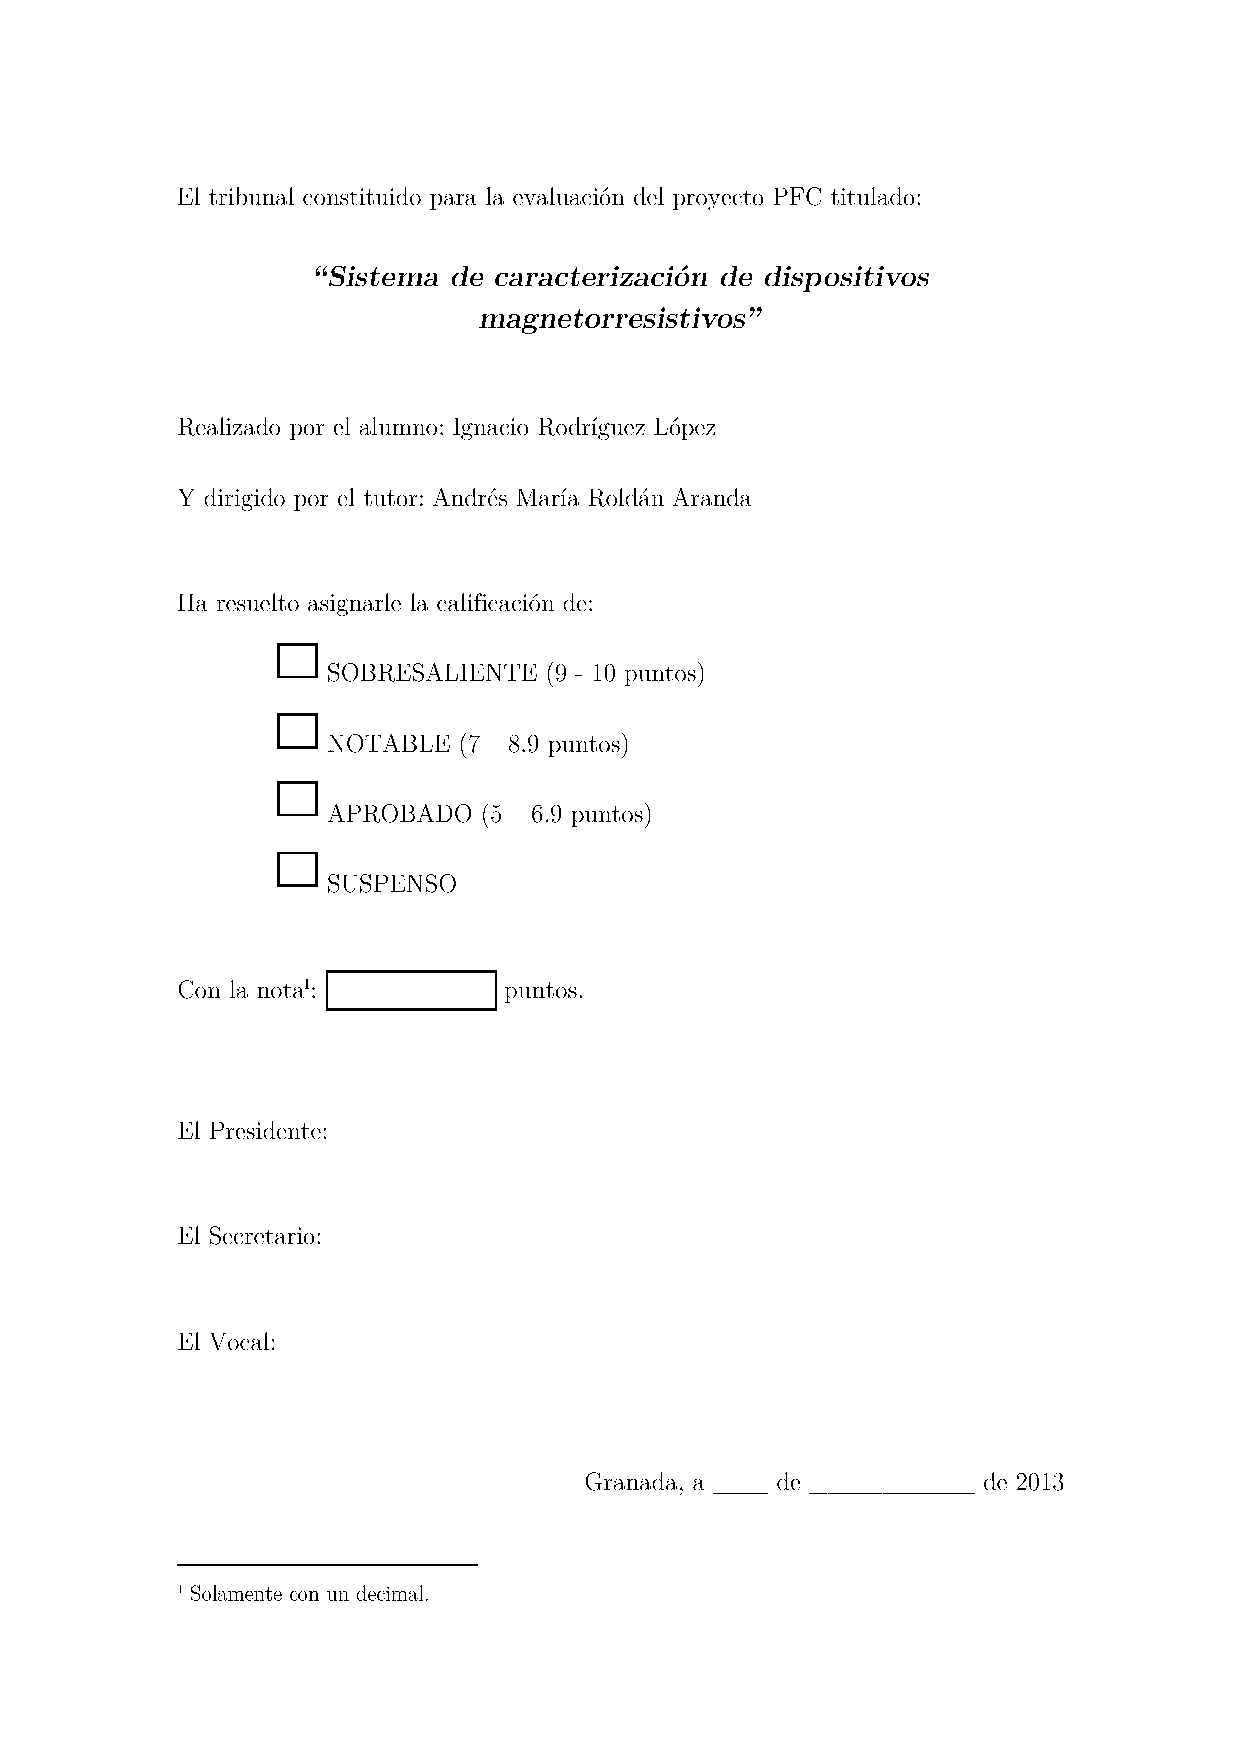
\includepdf[pages=-,link=true,linkname=hojaEvaluacionesUGR]{anexoIV_actaPFC}

\newpage
\thispagestyle{empty}

%Begin ----  Para que funcione bien el TOC en PDF
\cleardoublepage
\thispagestyle{empty}
\phantomsection
\addcontentsline{toc}{chapter}{Autorización Lectura}

\noindent D. Andrés María Roldán Aranda, Profesor del departamento
de Electrónica y Tecnología de los Computadores de la Universidad
de Granada, como director del Proyecto Fin de Carrera de D. Germán del Castillo Cuesta,

\vspace*{1cm}

Informa:

\begin{doublespace}
que el presente trabajo, titulado:
\end{doublespace}

\begin{doublespace}
\begin{center}
\textbf{\emph{\large {}``Control de temperatura en un horno con un microcontrolador''}}
\par\end{center}{\large \par}
\end{doublespace}

\noindent ha sido realizado y redactado por el mencionado alumno bajo
nuestra dirección, y con esta fecha autorizo a su presentación. 

\vspace*{1cm}

\begin{center}
%Granada, a 06 de Julio de 2012 
Granada, a ~~~~~~ de Junio de 2015
\par\end{center}

\bigskip%%%%%%%o
\bigskip%%%%%%%o
\begin{doublespace}
\hspace{4cm}Fdo.
\end{doublespace}

\newpage
\thispagestyle{empty}
\noindent

\newpage
\thispagestyle{empty}

~

%Begin ----  Para que funcione bien el TOC en PDF
\cleardoublepage
\phantomsection
\thispagestyle{empty}

\addcontentsline{toc}{chapter}{Autorización Depósito Biblioteca}

\noindent Los abajo firmantes autorizan a que la presente copia de
Proyecto Fin de Carrera se ubique en la Biblioteca del Centro y/o
departamento para ser libremente consultada por las personas que lo
deseen.

\vspace*{1cm}

\begin{center}
%Granada, a 06 de Julio de 2012
Granada, a ~~~~~~ de Junio de 2015
\par\end{center}

\bigskip%%%%%%%o
\bigskip%%%%%%%o
\begin{doublespace}
\hspace{4cm}Fdo.
\end{doublespace}

\newpage
\thispagestyle{empty}

~

%Begin ----  Para que funcione bien el TOC en PDF
\cleardoublepage
\phantomsection
\thispagestyle{empty}
\addcontentsline{toc}{chapter}{Resumen}

\begin{center}
\textbf{\Large Control de temperatura en un horno con un microcontrolador}
\par\end{center}{\Large \par}

\begin{center}
\textbf{\large Germán del Castillo Cuesta}
\par\end{center}{\large \par}

\vspace{0.75cm}






\begin{doublespace}
\noindent \textbf{PALABRAS CLAVE:}
\end{doublespace}



\begin{singlespace}
\noindent Arduino, PCB, PT100, PID, Matlab, Altium, Rotary Encoder, horno,SMD.

\end{singlespace}

\begin{doublespace}
\noindent \textbf{RESUMEN:}
\end{doublespace}

\begin{singlespace}

\noindent Este proyecto tendrá como objetivo la realización de un sistema de caracterización de dispositivos magnetorresistivos. El trabajo se concentrará en el diseño de un escenario capaz de posicionarse sobre dichos dispositivos e inducir en ellos un campo magnético homogéneo para analizar su comportamiento resistivo. El sistema incorporará un software específico para configurar el conexionado del sistema y lanzar el procedimiento de medida, controlando la instrumentación involucrada mediante buses GPIB y RS-232.
%Desarrollo de un sistema de control de puertas abatibles. El sistema estar? orientado hacia la unificaci?n en un solo producto de los distintos escenarios que existen en la realidad. Se dise?ar? el sistema completo, incluyendo desarrollos a nivel hardware y firmware. La recepci?n de las se?ales se har? desde un telecommando a la frecuencia reservada para ello.
\end{singlespace}

\vspace{1.25cm}


\begin{doublespace}
\noindent \textbf{KEYWORDS:}
\end{doublespace}

\begin{singlespace}
%\noindent Printed Circuit Board (PCB), control box, flap, RF communication, automation, microcontroller.
\noindent Magnetoresistance, sensors, magnetic field, Helmhotz's coils, current strap, characterisation, probe station, head probes, gaussmeter, Hall probes, Matlab, GPIB, RS-232, automation, simulation, remote control, electronic instrumentation, parameter analyzer, PCB.
\end{singlespace}

\begin{doublespace}
\noindent \textbf{ABSTRACT:}
\end{doublespace}

\begin{singlespace}
\noindent This project will develop a magnetoresistance devices characterisation system. This work will be focused on the design of an stage capable of positioning over these devices while inducing an homogeneous magnetic field on them in order to analyse their resistive behavior. The system will also integrate a specific software to assist the setup procedure as well as for triggering the measurement, remotely controlling all the involved intrumentation through GPIB and RS-232 buses. 
%\noindent Development of a folding door control. The system will be geared towards the unification into a single product of the different scenarios that exist in reality. It will design the entire system, including developments at the hardware and firmware. Receiving signals from a telecomm will the frequency reserved for it.
\end{singlespace}


\newpage
\thispagestyle{empty}

~

%Begin ----  Para que funcione bien el TOC en PDF
\cleardoublepage
\phantomsection
\thispagestyle{empty}
\addcontentsline{toc}{chapter}{Dedicatoria}

\vspace{6cm}

\begin{quotation}
\noindent \begin{center}
\textbf{\emph{\Large Dedicado a}}\textbf{\emph{\large }}\\
\textbf{\emph{\large }}\\
\textbf{\emph{\large }}\\
\textbf{\emph{\large Mis padres, Germán y Antonia. Sin ellos nada de esto hubiera sido posible.}}
%\textbf{\emph{\large .....Esto lo último.....}}
%Todos aquellos que no tuvieron la oportunidad.
\par\end{center}{\large \par}
\end{quotation}
\newpage
\thispagestyle{empty}

~\newpage
\thispagestyle{empty}




%%Agradecimientos 
   %Begin ----  Para que funcione bien el TOC en PDF
\cleardoublepage
\phantomsection
\addcontentsline{toc}{chapter}{Agradecimientos}

\vspace*{2.5cm}


\begin{quotation}
\noindent \begin{center}
\textbf{\emph{\Large Agradecimientos:}}\textbf{\emph{\large }}\\
\textbf{\emph{\large }}\\
\textbf{\emph{\large }}\\
\textbf{\emph{\large }}
\par\end{center}{\large \par}
\end{quotation}

\begin{onehalfspace}

Una carrera universitaria es una etapa de la vida, tal vez aquella en la que se tiene la máxima libertad para hacerse a uno mismo, y en ello influyen todas las personas que nos rodean. He tenido la suerte de tener a mi lado a los mejores, y les debo mi eterno agradecimiento a todos.

A Papá y Mamá, por la vida y el cariño. A Laura, por ser la mejor hermana. A Daniel y Francisco, por las risas. A Paco y José Antonio, por ir un paso por delante. A Manolo y Jesús, por la Alianza. A la Peñita de Milán, por el Erasmus. A los Milestones, por la música. A Mariadel, por enseñarme a tocar el piano. Y a Salva, por explicarme lo que era un ordenador.

También quiero expresar mi agradecimiento a todos los profesores de la Universidad de Granada por su inestimable esfuerzo por formarnos, así como a todas las personas implicadas en este proyecto: D. Andrés Roldán Aranda, mi tutor, Mikel Aguayo Fernández, ingeriero de la PCB, y el organista Juan Rodríguez Ruiz, nuestro más valioso colaborador.

\end{onehalfspace}

%\bigskip
%Todos son igualmente partícipes de este trabajo.

\clearpage{\pagestyle{empty}\cleardoublepage}%

%
%%Lista de FIGURAS
   
%\pagenumbering{roman}%

\pagestyle{fancy}%
\clearpage{\pagestyle{plain}\cleardoublepage}%

%Begin ----  Para que funcione bien el TOC en PDF
\cleardoublepage
\phantomsection \label{tableofcont}
%END  ---- Para que funcione bien el TOC en PDF

\begin{singlespacing}%onehalfspacing}
\tableofcontents
\end{singlespacing}%onehalfspacing}




%Begin ----  Para que funcione bien el TOC en PDF
\cleardoublepage
\phantomsection \label{listoffig}
%END  ---- Para que funcione bien el TOC en PDF
 
\begin{singlespacing}%onehalfspacing}
\listoffigures
\end{singlespacing}%onehalfspacing}


%\fancyhead{}
%\fancyhead[RO]{\small{\nouppercase{Índice de Figuras}}}
%\fancyhead[LE]{\small{\nouppercase{Índice de Figuras}}}

%\addcontentsline{toc}{chapter}{Lista de Figuras}%

\clearpage{\pagestyle{fancy}\cleardoublepage}%

%
%%Lista de FIGURAS
%   %Begin ----  Para que funcione bien el TOC en PDF
\cleardoublepage
\phantomsection \label{listings}
\addcontentsline{toc}{chapter}{Indice Listados}
%END  ---- Para que funcione bien el TOC en PDF
\begin{singlespacing}%onehalfspacing}
\lstlistoflistings
\end{singlespacing}%onehalfspacing}


%\fancyhead{}
%\fancyhead[RO]{\small{\nouppercase{Índice de Listados}}}
%\fancyhead[LE]{\small{\nouppercase{Índice de Listados}}}

%\addcontentsline{toc}{chapter}{Lista de Figuras}%

\clearpage{\pagestyle{fancy}\cleardoublepage}%

%
%%Lista de TABLAS
   %Begin ----  Para que funcione bien el TOC en PDF
\cleardoublepage
\phantomsection \label{Tablass}
%\addcontentsline{toc}{chapter}{Índice Tablas}
%END  ---- Para que funcione bien el TOC en PDF
\begin{singlespacing}%onehalfspacing}
\listoftables
\end{singlespacing}%onehalfspacing}

%
%\fancyhead{}
%\fancyhead[RO]{\small{\nouppercase{Índice de Tablas}}}
%\fancyhead[LE]{\small{\nouppercase{Índice de Tablas}}}

%\addcontentsline{toc}{chapter}{Lista de Tablas}%

\clearpage{\pagestyle{fancy}\cleardoublepage}%





%%%Símbolos: se incluyen en el listado de símbolos
%      \gls{pi}, \gls{ohm}, \gls{angstrom}, 
%      \gls{QIPrima},    \gls{QBPrima},    \gls{QGPrima}
%      \gls{QI},    \gls{QB},    \gls{QG}   
%      \gls{qI},    \gls{qB},    \gls{qG}   
%      \gls{Idb},    \gls{gm},    \gls{gmb},    \gls{gsd}   
%      \gls{gbg},    \gls{gbs},    \gls{gbd}         
%
%Acrónimos
%\acrshort{SMD} (\acrlong{SMD})
%Enlace al glosario
%\glsname{HISIM} (\glstext{HISIM})
%
%%%%%% ERROR  %%%%%%%
%\acrshort{EKV} %(\acrlong{CRA})
%\glsname{EKV} (\glstext{EKV})

%%Citas: hace un enlace a la Bibliografía
%\cite{rytter1993vibration}
%\cite{frietzen2002CFRP}
%\cite{chang1999SHM}



%Capítulo 1: Introducción
\chapter{Introducción y objetivos}
\label{cap:capitulo_1}
\pagenumbering{arabic}

\begin{quote}
	\small \flushright ''\textit{Una partitura también es un lenguaje.}'' \\
	--- Profesor Buenaventura Clares Rodríguez (2013).
\end{quote}

\vspace{4em}

\section{Contexto}

Llegado el momento de cursar la asignatura ''Proyectos Informáticos'' de la titulación, iniciamos los preparativos para desarrollar un proyecto propuesto por el Departamento de Electrónica y Tecnología de Computadores de la Universidad de Granada.

Para plantearlo, nos hemos fijado en numerosas iglesias de Granada, que incorporan órganos de tubos, instrumentos muy complejos, muchos de ellos formando parte del inmobiliario, y merecedores de un gran reconocimiento por la artesanía y la calidad de su construcción. Lamentablemente, muchos de ellos están en un estado de abandono, debido principalmente a que si no se tocan regularmente, se deterioran y no se reparan, y al no hacerlo, no se pueden tocar, cayendo en un círculo vicioso.

Además, creemos interesante la idea de que se pueda hacer sonar un órgano aunque no haya organista, dando la posibilidad tanto de acompañar celebraciones litúrgicas como de tener música de fondo durante el horario de visitas.

\section{Objetivos}

Nuestro propósito es ingeniar un sistema capaz de \textbf{interpretar partituras musicales en un órgano} suplantando las pulsaciones del artista, lo que incluye los siguientes objetivos:

\begin{enumerate}
	\item Analizar la \textbf{mecánica real} de un órgano.
	
	\begin{enumerate}
		\item Tomar \textbf{medidas completas} de cada uno de los teclados, los pedales y las palancas de registros.
		\item \textbf{Diseñar en 3D} los componentes principales del instrumento.
		\item Determinar la \textbf{presión} necesaria para mover cada tecla, cada pedal y cada palanca del órgano.
	\end{enumerate}
	
	\item Estudiar la comunicación entre el \textit{software} y el \textit{hardware}, incluyendo todos los \textbf{componentes electrónicos} que habrá de incluir.
	
	\item Plantear distintas \textbf{alternativas de sistemas empotrados} que sirvan de soporte de programación.
	
	\item Analizar el \textbf{protocolo \acrshort{MIDI}} como formato de archivo para almacenar partituras.
	
	\item \textbf{Diseñar} el sistema \textit{software} que cubrirá varias vías de comunicación entre el usuario y la mecánica, lo que comprende:
	
	\begin{enumerate}
		\item Un \textbf{servicio en segundo plano}, que atienda:
		
		\begin{enumerate}
			\item Reproducción de archivos \acrshort{MIDI}.
			\item Comunicación inter-proceso.
			\item Receptor de un mando a distancia.
			\item Menú de control sobre el hardware, con un ''modo Ingeniería''.
		\end{enumerate}
		
		\item Una \textbf{aplicación \textit{web}} para controlar el sistema, con soporte para:
		
		\begin{enumerate}
			\item Reproducir partituras electrónicas.
			\item Instalar nuevas piezas y gestionar listas de reproducción.
			\item Configurar el mando a distancia.
		\end{enumerate}
		
		\item Una \textbf{base de datos} como soporte de almacenamiento persistente.
		\item Un \textbf{protocolo de comunicación} entre la aplicación y el servicio.
	\end{enumerate}
	
	\item \textbf{Implementar} el sistema diseñado, como:
	
	\begin{enumerate}
		\item Un demonio para Linux.
		\item Un servicio \textit{web} sobre Apache y \acrshort{PHP}.
		\item Una base de datos MySQL.
	\end{enumerate}
	
	\item \textbf{Validar} junto al \textit{hardware} el proyecto desarrollado.
\end{enumerate}

Este proyecto atenderá al objetivo global pero \textbf{el desarrollo se centrará en la parte \textit{software}}, ya que el \textit{hardware} requiere competencias de Ingeniería Electrónica e Industrial, y será objeto del proyecto de D. Mikel Aguayo Fernández.

Para abordarlo, hemos contado con la colaboración de \textbf{Juan Rodríguez Ruiz}, responsable del órgano de la \textbf{Parroquia de la Encarnación de Santa Fe}, que nos ha dado acceso tanto al instrumento como a asombrosos datos sobre su historia y su construcción.

\smallskip

\begin{figure}[H]
\noindent \begin{centering}
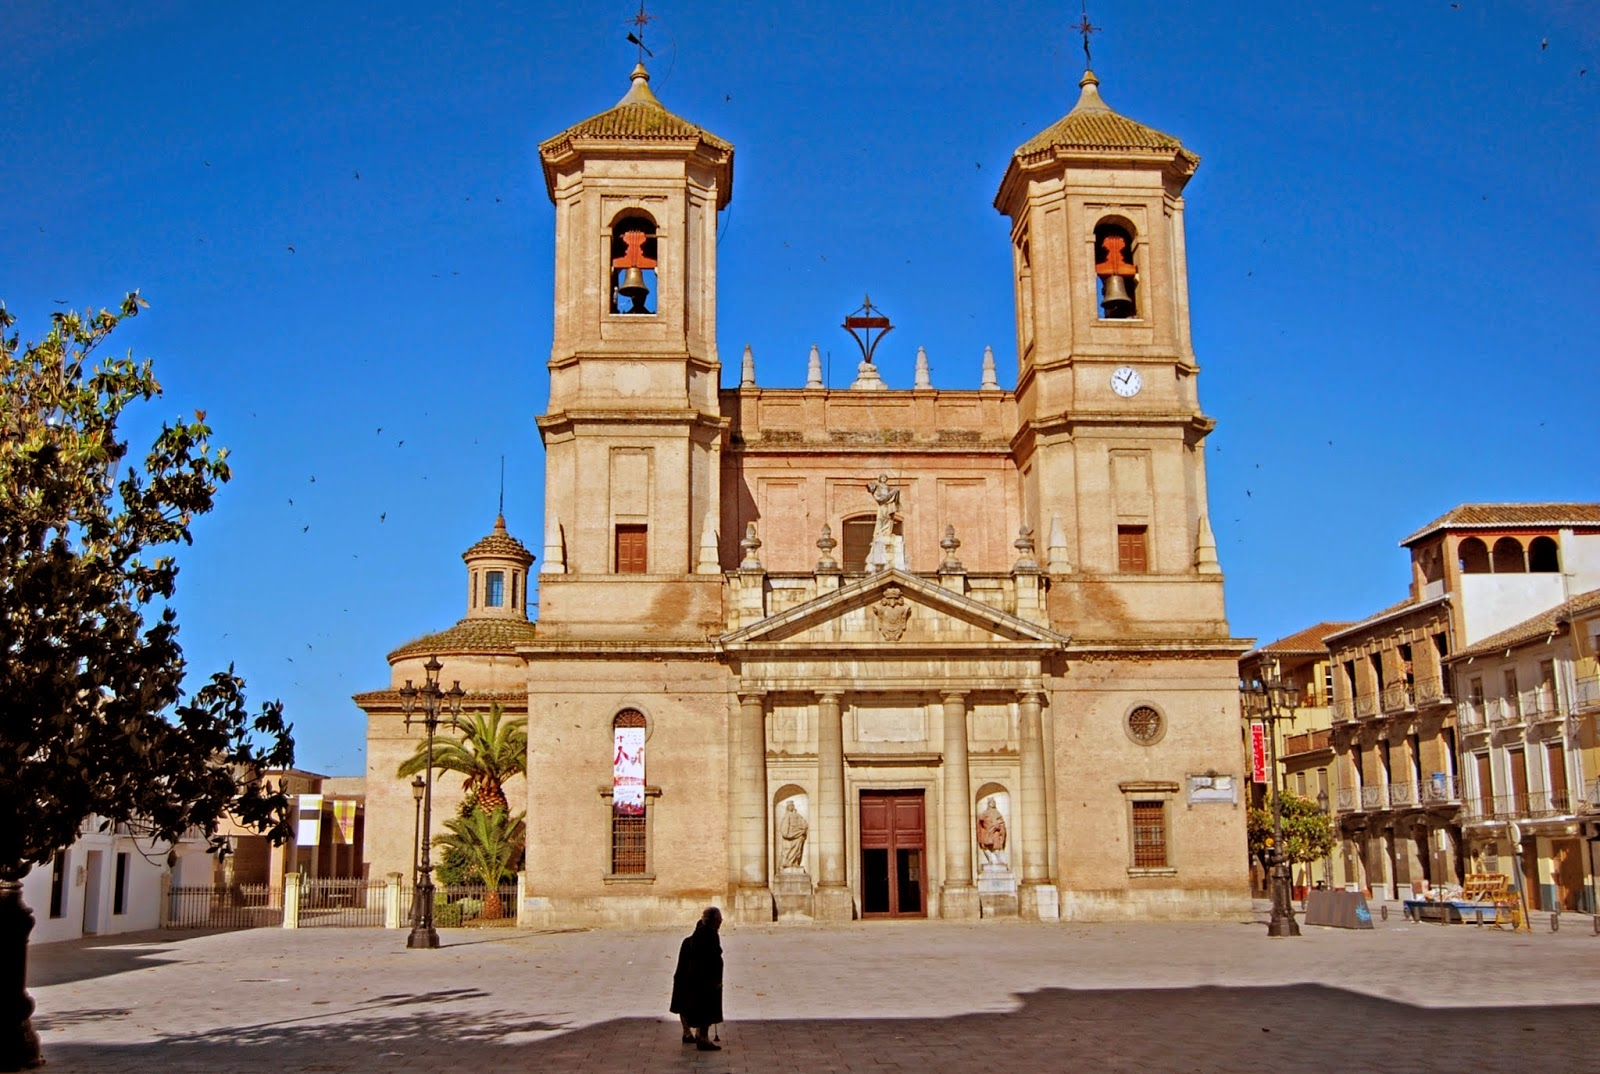
\includegraphics[width=\linewidth]{capitulo1/figura11}
\par\end{centering}
\smallskip
\caption[Parroquia de la Encarnación de Santa Fe.]{\label{fig:figura11} Parroquia de la Encarnación de Santa Fe. \cite{iglesias_granada}}
\end{figure}

\newpage

\section{Contenido y estructura capitular}

Una vez planteado el problema, utilizaremos el \textbf{modelo de desarrollo en cascada} para continuar el resto del proyecto.

El modelo en cascada ordena rigurosamente las etapas del proceso, de forma que cada tarea se inicia cuando su precedente finaliza, tal como se expone en la siguiente ilustración:

\smallskip

\begin{figure}[H]
	\noindent \begin{centering}
		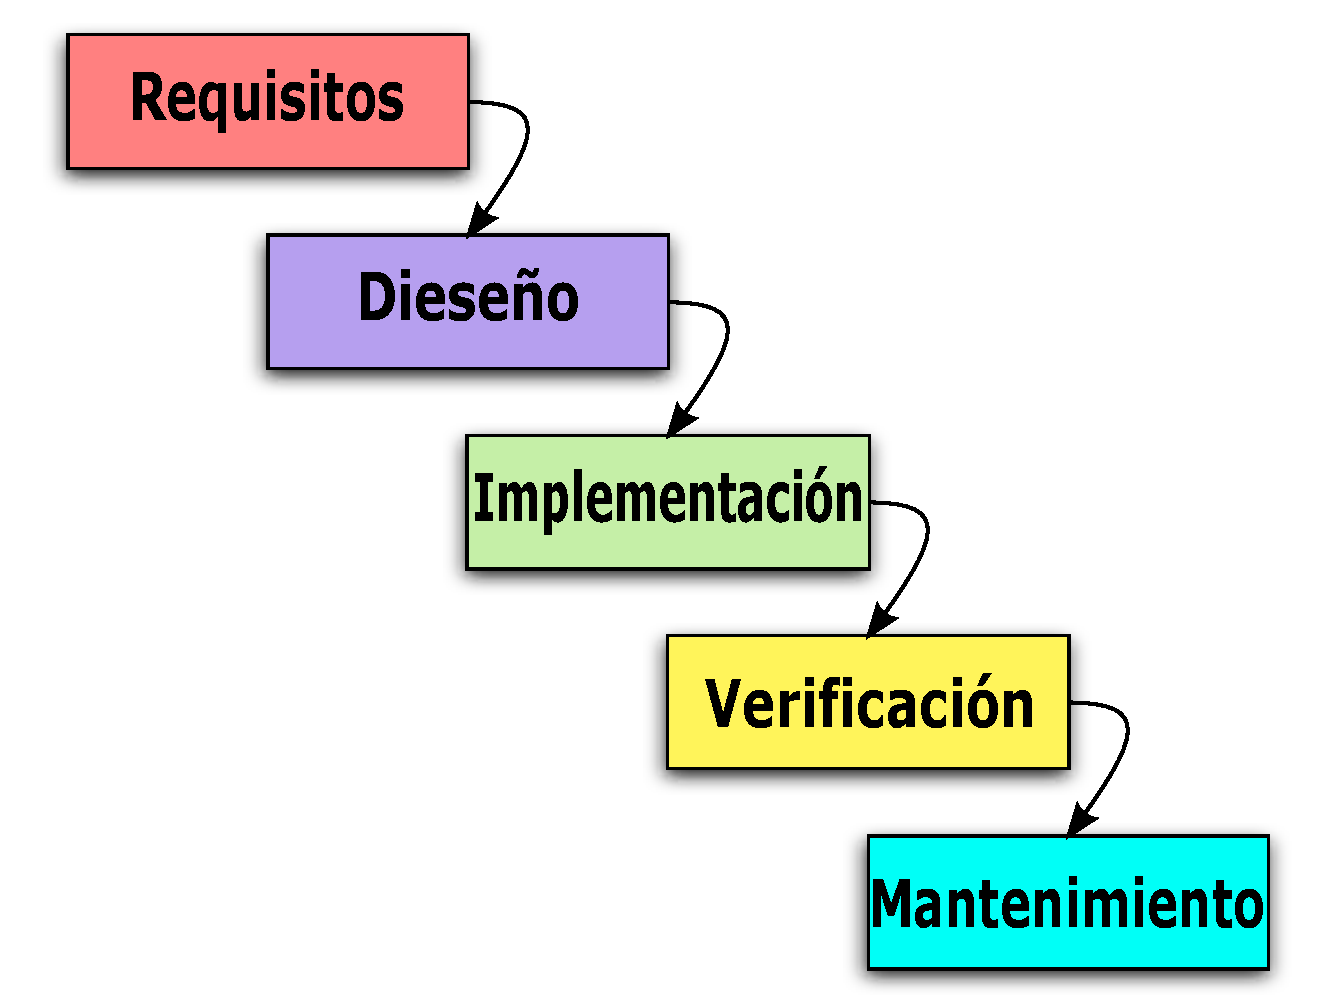
\includegraphics[width=\linewidth/2]{capitulo1/figura12}
		\par\end{centering}
	\smallskip
	\caption[Modelo de desarrollo en cascada.]{\label{fig:figura12} Modelo de desarrollo en cascada. \cite{wiki_cascada}}
\end{figure} 

\smallskip

Basándonos en la figura anterior, definiremos el resto de capítulos de esta memoria.

\begin{itemize}

\item \textbf{Capítulo 2:} En este capítulo especificaremos los requisitos que supone el diseño del sistema para alcanzar nuestro objetivo, así como indicar las fases del proyecto.

\item \textbf{Capítulo 3:} Vamos a analizar todos los elementos con los que vamos a interactuar, desde el teclado del órgano hasta el computador sobre el que funcionará nuestro \textit{software}. 

\item \textbf{Capítulo 4:} Plantearemos el diseño de la solución, haciendo Ingeniería el \textit{software}, que cumpla de la mejor manera posible los requerimientos del \ref{cap:capitulo_2}.

\item \textbf{Capítulo 5:} En esta parte explicaremos cómo hemos implementado la solución diseñada, y cómo hemos enfrentado los principales problemas que han surgido.

\item \textbf{Capítulo 6:} Vamos a validar el sistema poniéndolo en funcionamiento y probando que cumple los requisitos propuestos.

\item \textbf{Capítulo 7:} Expondremos la conclusión y las posibilidades que nos brinda el proyecto de cara al futuro.
  
\end{itemize}

\newpage
\clearpage{\pagestyle{empty}\cleardoublepage}


%Capítulo 2: Requisitos previos
\chapter{Requisitos técnicos}
\label{cap:capitulo_2}

\begin{quote}
	\small \flushright ``\textit{Requisito no funcional nº 1: El diseño del sistema debe ser correcto.}'' \\
	--- Profesor José Parets Llorca (2013).
\end{quote}

\vspace{8em}

Como hemos adelantado, pretendemos diseñar un sistema autónomo capaz de hacer sonar un órgano de tubos, tal como lo haría un artista. El uso está enfocado a minimizar la interacción del usuario con el sistema. 

Para especificar el diseño de este proyecto hemos propuesto una serie de requisitos tanto \textit{hardware} como \textit{software}, que enumeramos a continuación.

\newpage 

\section{Requisitos hardware}

\begin{enumerate}
	
	\item Un juego de mecanismos accionará las \textbf{teclas}, otro moverá los \textbf{pedales} y otro desplazará los \textbf{registros} de timbres.
	
	\item El sistema no podrá acceder a la mecánica interna del instrumento, ni modificarlo de ninguna forma.
	
	\item No podrá apoyarse demasiado peso sobre el órgano, ni hacerse contra-apoyo (hacia arriba).
	
	\item El \textbf{control principal}, la instalación de partituras y la configuración se harán \textbf{remotamente}.
	
	\item Se proveerá un \textbf{control local reducido} de los accionadores con fines de puesta en marcha y mantenimiento.
	
	\item Asimismo se facilitará el control remoto desde un \textbf{mando a distancia}.
	
	\item El diseño debe ser \textbf{flexible y extensible} para distintos órganos.
	
	\item Se debe de poder instalar y desinstalar fácilmente.
	
\end{enumerate}

\section{Requisitos software}

Teniendo en cuenta los requisitos \textit{hardware} y el perfil del usuario final, planteamos los siguientes requisitos para el \textit{software} a diseñar:

\begin{enumerate}

	\item Se ofrecerá \textbf{control remoto} para todos los casos de uso a nivel de usuario.
	
	\item La interfaz permitirá controlar la \textbf{reproducción}: iniciar una pieza, pausarla, reanudarla y detenerla. La reproducción por defecto será en modo bucle.
	
	\item Facilitará la subida y \textbf{gestión de partituras}. En dicho gestor se mostrará la duración de cada pieza.
	
	\item Los archivos a procesar son de formato \textbf{\acrshort{MIDI} estándar}, sin perjuicio de que una partitura pueda estar adaptada específicamente al sistema.
	
	\item Las piezas musicales se clasificarán en \textbf{listas de reproducción}.
	
	\item La interfaz de usuario permitirá \textbf{asignar} dichas listas a ciertos botones del mando arriba mencionado.
	
	\item El \textbf{mando} tendrá capacidad para reproducir una serie de listas pre-programadas, así como pausar y detener la reproducción.
	
	\item El \textit{software} dará soporte al \textbf{testeo} de los accionadores de forma local.
	
	\item El controlador debe ser \textbf{extensible} para órganos con más o menos teclas, distinto número de teclados o diferente configuración de registros.
	
	\item La aplicación para el usuario debe ser lo más \textbf{sencilla e intuitiva} posible.
	
	\item Se busca obtener una aplicación de control \textbf{multiplataforma}.
	
	\item La interfaz de usuario se presentará en varios \textbf{idiomas}.
	
	\item Ya que el control es remoto, se hará hincapié en la \textbf{seguridad}, tanto autentificación de acceso como aspectos de programación, tales como inyección de código.

\end{enumerate}

\newpage

\section{Fases del proyecto}

Tal como hemos introducido anteriormente, vamos a dividir este proyecto en cuatro fases, cada una de las cuales servirá para obtener los requisitos necesarios para continuar la siguiente. Vamos a trabajar de la siguiente forma:

\begin{enumerate}
	\item \textbf{FASE I --- Análisis:} Vamos a estudiar todos los componentes a los que tenemos acceso, desde el órgano hasta la placa de circuito y el computador a utilizar, pasando por la especificación del formato \acrshort{MIDI}.
	
	\item \textbf{FASE II --- Diseño:} En esta fase reunimos las especificaciones del sistema y los requisitos propuestos para definir el sistema que vamos a concebir, desde la interfaz al usuario hasta la interacción con el \textit{hardware}.
	
	\item \textbf{FASE III --- Implementación:} Es la etapa en la que se programa el \textit{software} a partir del diseño de la fase precedente, y prestaremos atención a los detalles de bajo nivel que se nos presentarán, desde llamadas al sistema y acceso a los periféricos hasta control de concurrencia.
	
	\item \textbf{FASE IV --- Verificación y validación:} Una vez terminada la fase de implementación, pondremos en funcionamiento el sistema para verificar que tanto el \textit{hardware} como el \textit{software} se integran correctamente y cumplen con los requisitos propuestos.
	
\end{enumerate}

\section{Planificación}

En base a nuestro objetivo final, este proyecto está estrechamente relacionado con el de Mikel Aguayo Fernández, que abordará la parte relacionada con \textit{hardware}.

Nuestro diseño será genérico para cualquier órgano pero \textbf{específico para la plataforma} \textit{hardware}. Por tanto, hay una parte del sistema que no se puede diseñar hasta conocer el proyecto de la \acrshort{PCB}. Para realizar una correcta planificación es necesario tener en cuenta qué parte de nuestro diseño depende del de Mikel Aguayo.

\subsection{Dependencias entre tareas}

Esencialmente tenemos los siguientes puntos en común:

\begin{enumerate}
	\item Compartimos inicialmente los \textbf{requisitos}, para entonces clasificarlos entre nuestros proyectos.
	\item El otro proyecto necesita el \textbf{análisis} realizado sobre el órgano.
	\item El nuestro, a su vez, depende del \textbf{diseño} que se haga de la \acrshort{PCB}.
	\item La \textbf{verificación} vuelve a poner en común nuestros trabajos.
\end{enumerate}

La siguiente figura descompone a \textit{grosso modo} las tareas e ilustra las \textbf{dependencias} encontradas:

\smallskip

\begin{figure}[H]
	\noindent \begin{centering}
		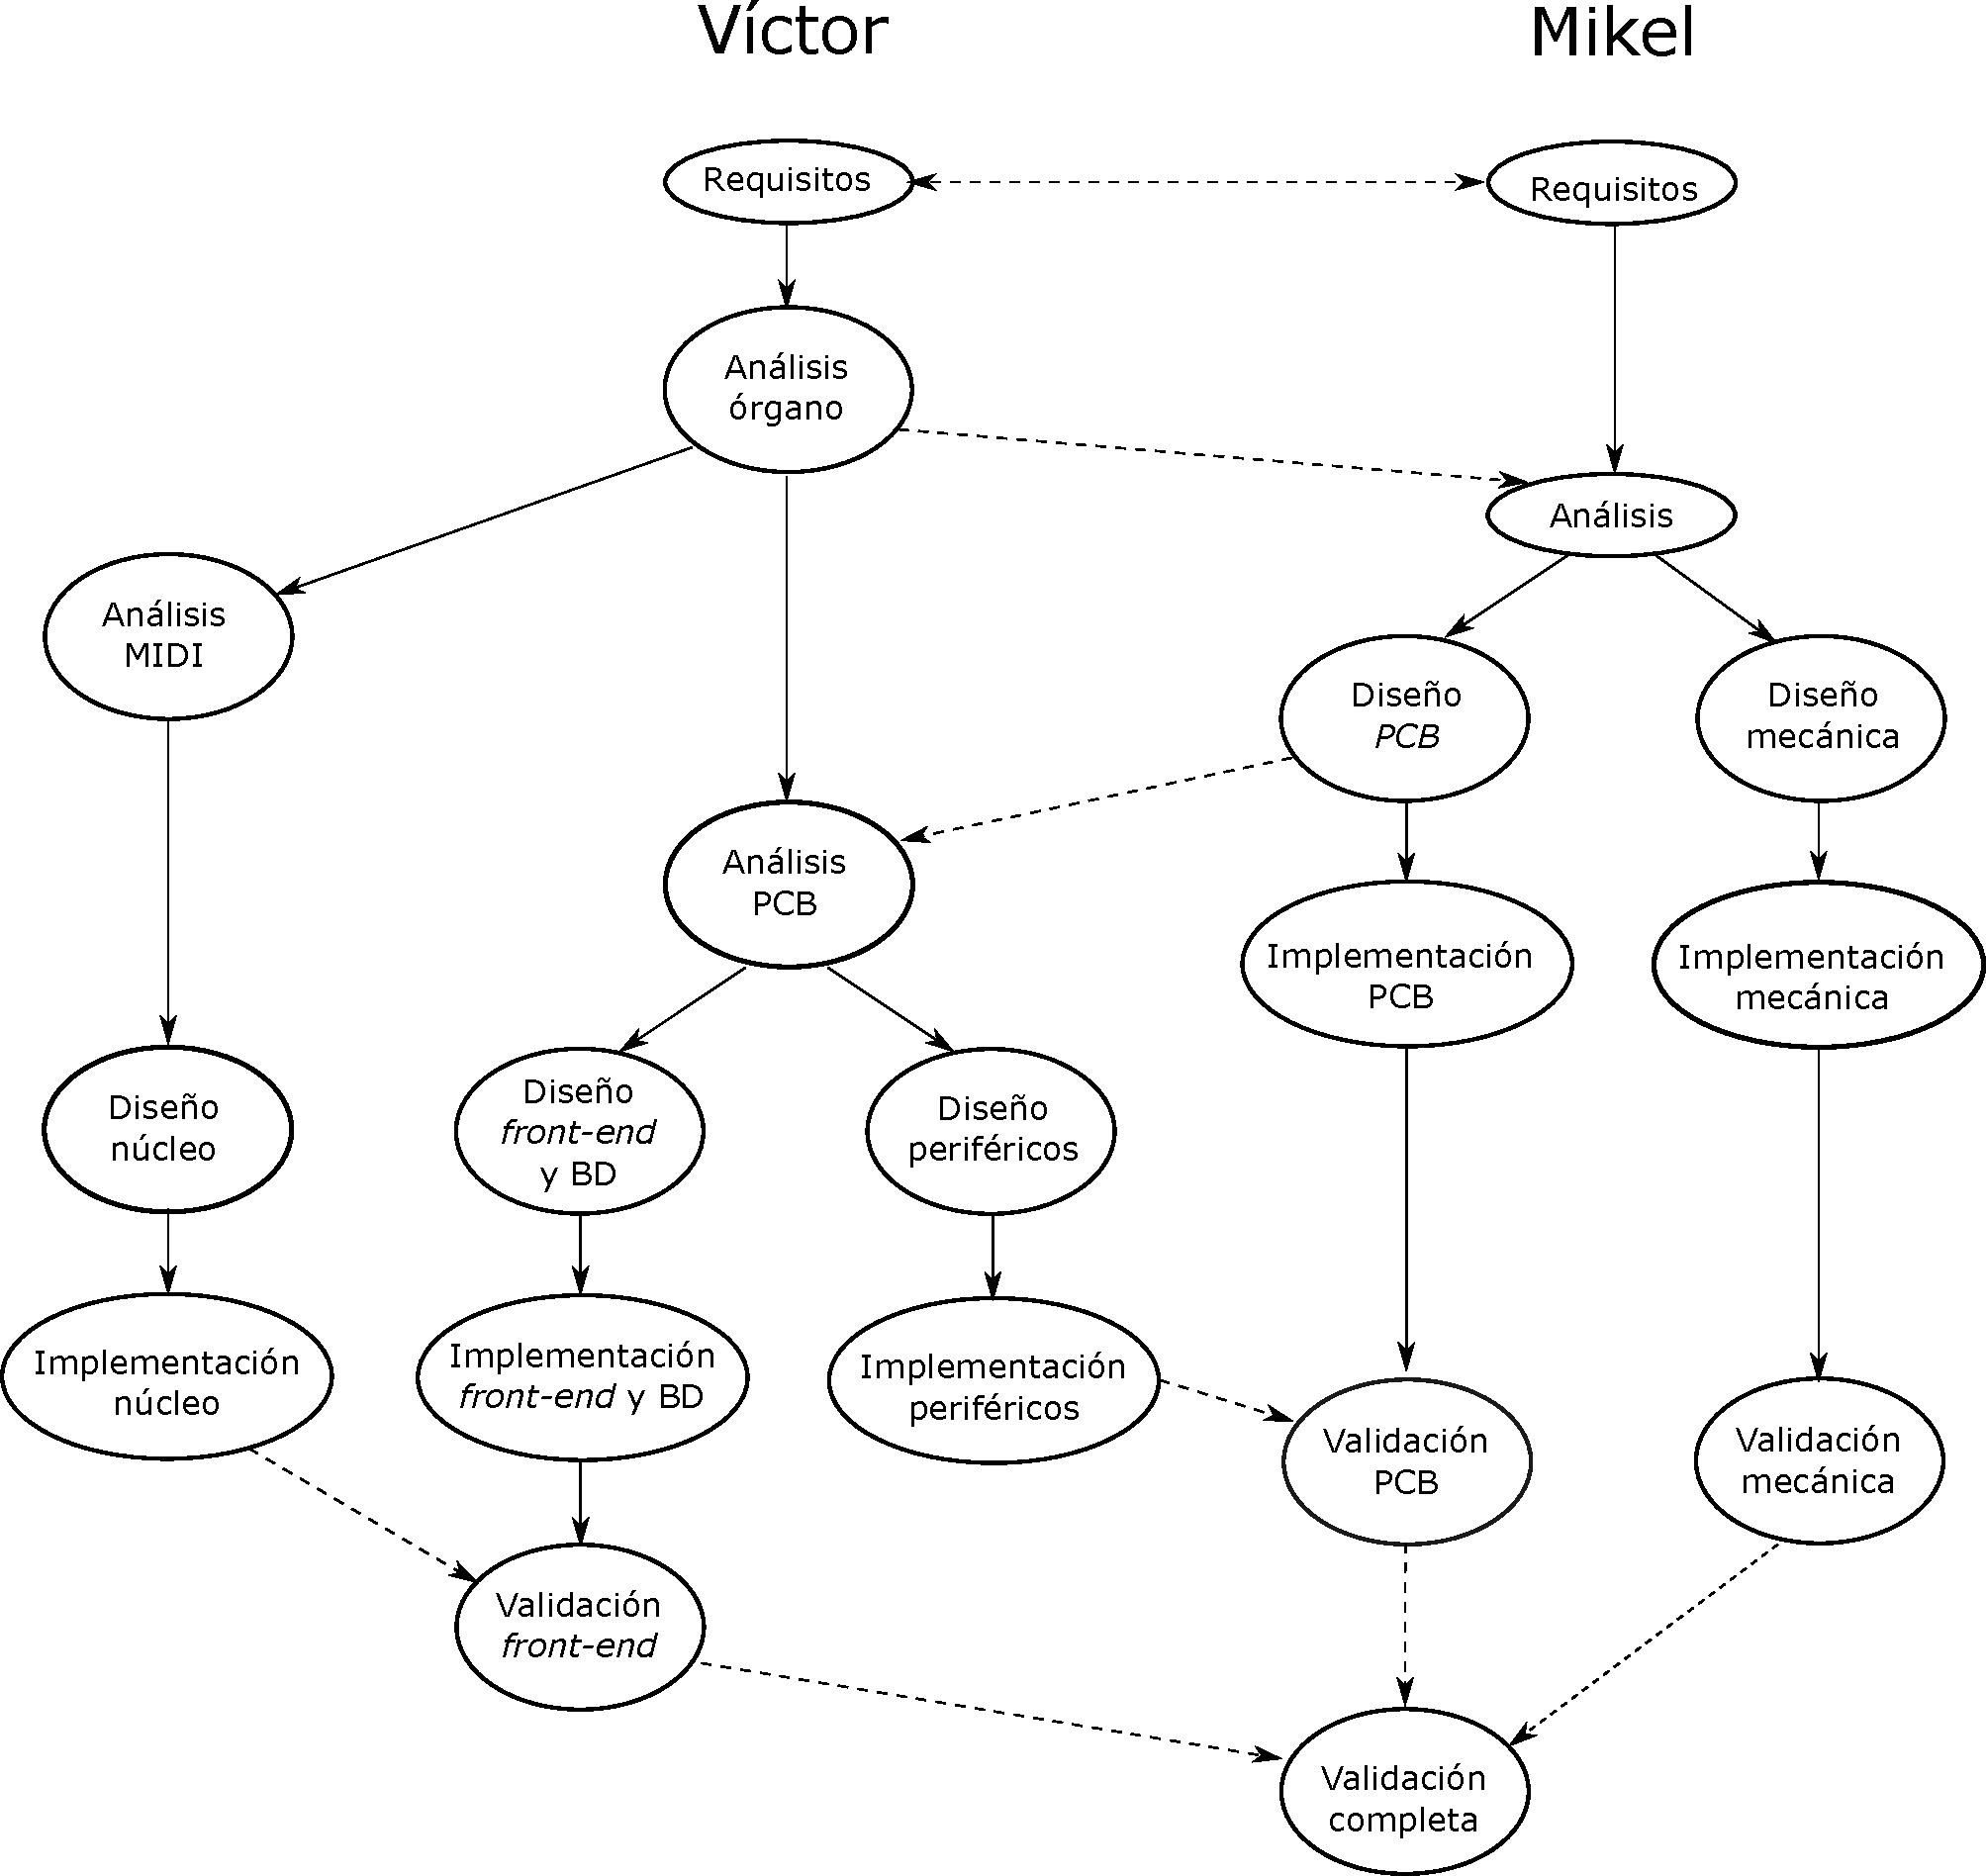
\includegraphics[width=\linewidth]{capitulo2/planificacion}
		\par\end{centering}
	\smallskip
	\caption{\label{fig:planificacion} Diagrama de dependencia de tareas.}
\end{figure} 

\newpage

A la vista de este diagrama, esbozaremos la \textbf{planificación temporal} de esta forma:

\smallskip

\begin{figure}[H]
	\noindent \begin{centering}
		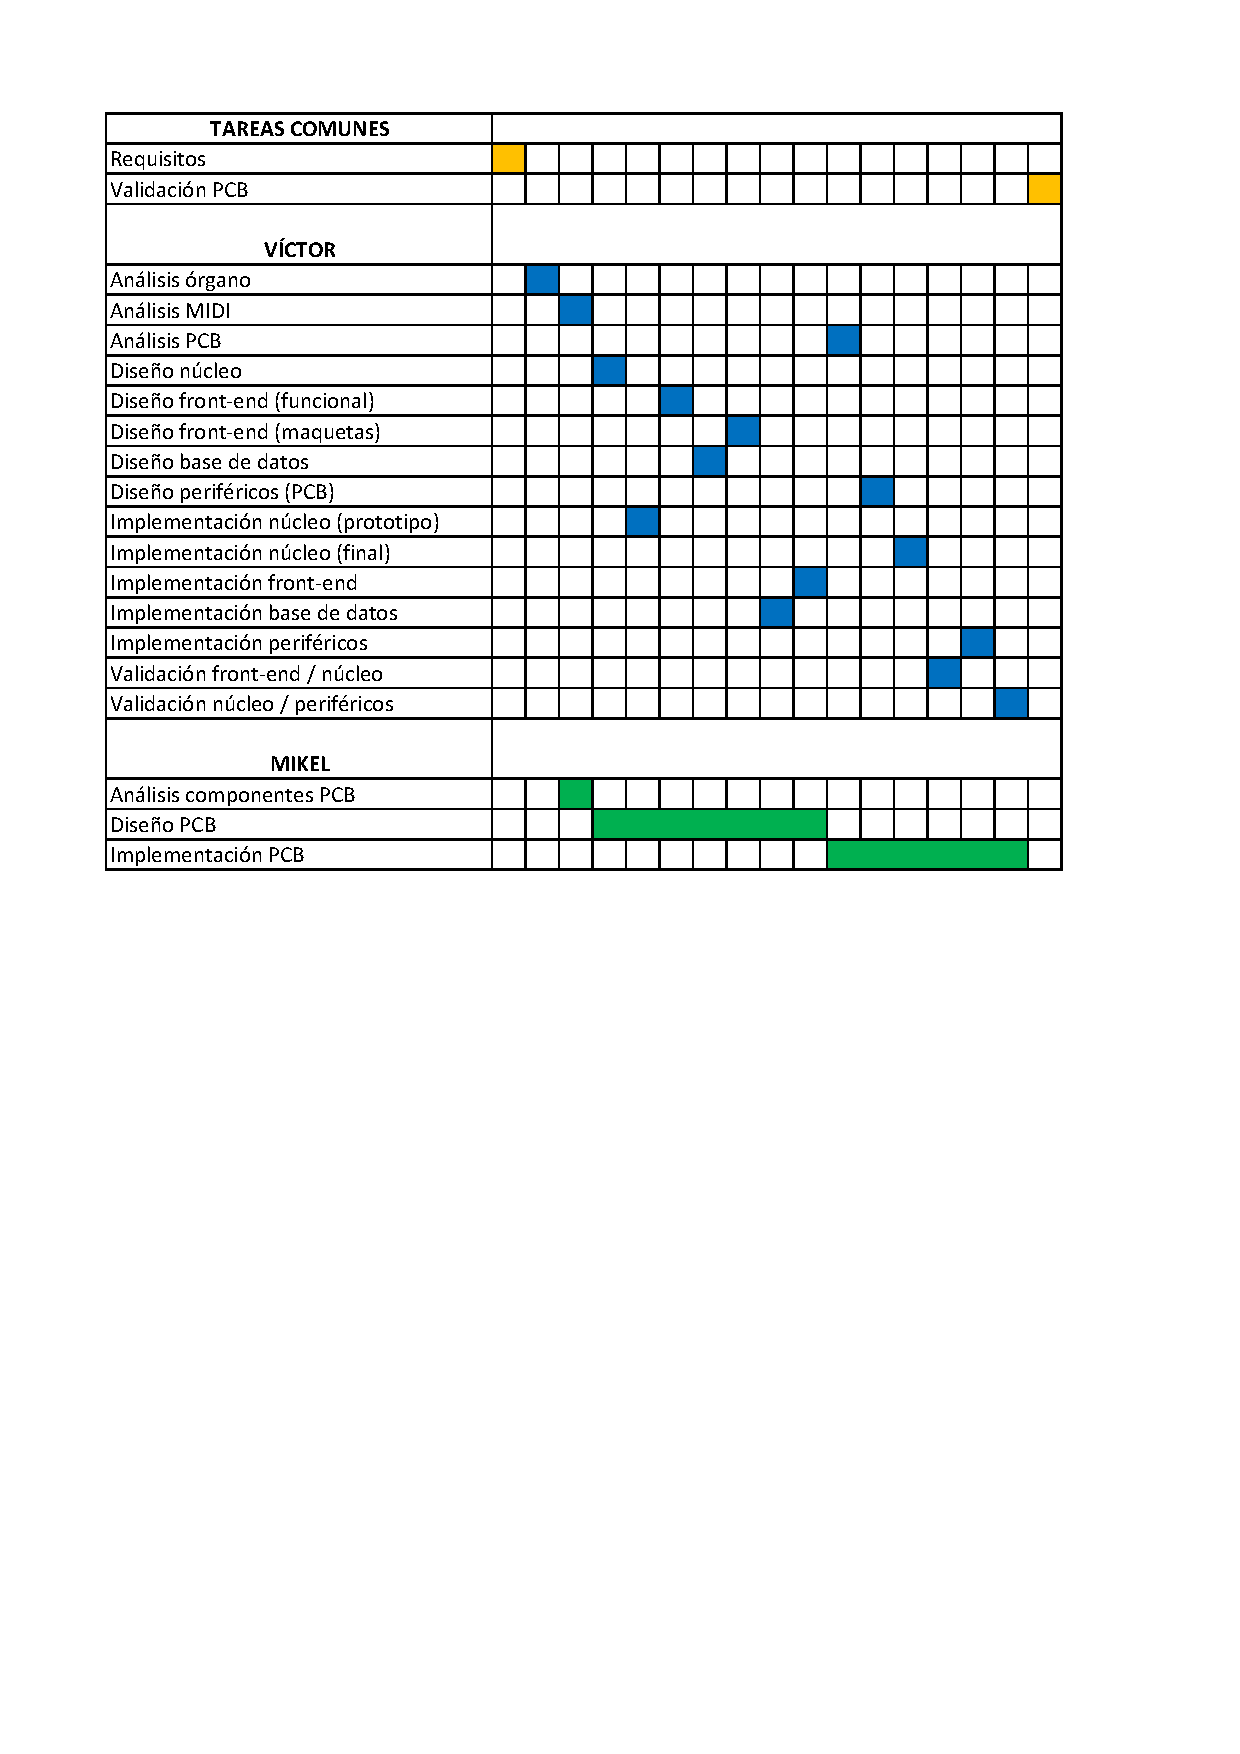
\includegraphics[width=\linewidth]{capitulo2/plan_gantt}
		\par\end{centering}
	\smallskip
	\caption{\label{fig:plan_gantt} Diagrama de Gantt básico.}
\end{figure} 

\smallskip

\subsection{Planificación prevista}

Conocidas las tareas básicas a realizar, proponemos la siguiente planificación para todos los bloques a desarrollar en el sistema. Hemos asignado principalmente las tareas por \textbf{semanas}, aunque algunas de ellas se podrán hacer en común por su simplicidad, y otras deberemos \textbf{descomponerlas} en prototipo e implementación final.

El primer paso es \textbf{analizar} el funcionamiento y la mecánica del órgano para permitir a Mikel continuar su trabajo. Mientras él diseña la \acrshort{PCB}, nosotros comenzamos el \textbf{diseño} de los módulos que no dependen de ésta. Tan pronto como recibamos su diseño, podremos desarrollar el resto del sistema.

\newpage

\begin{figure}[H]
	\noindent \begin{centering}
		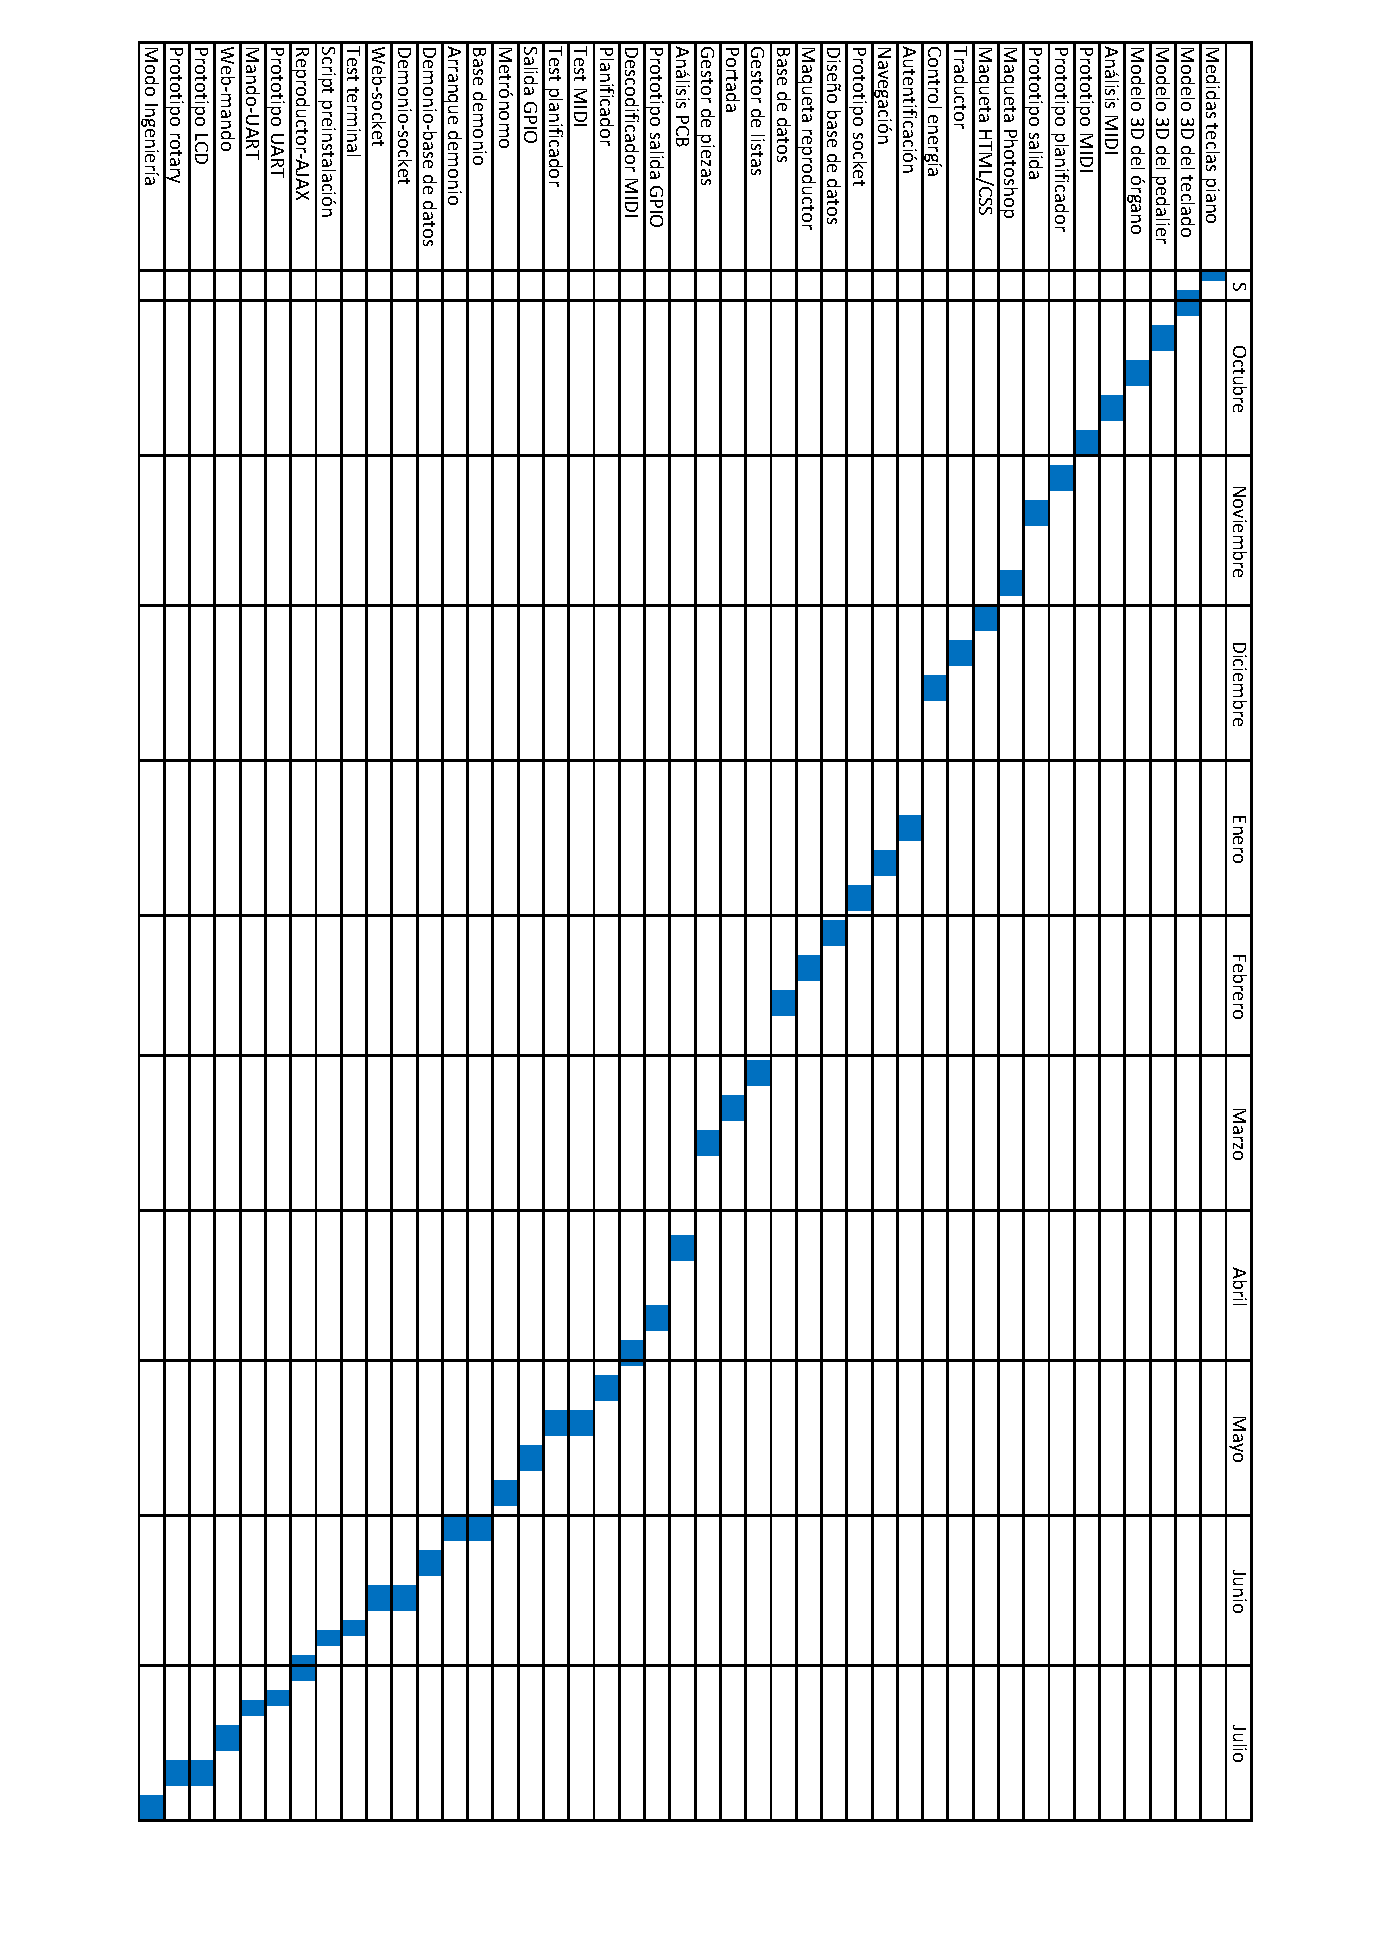
\includegraphics[height=\textheight]{capitulo2/gantt}
		\par\end{centering}
	\smallskip
	\caption{\label{fig:gantt} Diagrama de Gantt para planificación.}
\end{figure} 

\smallskip



\newpage
\clearpage{\pagestyle{empty}\cleardoublepage}


%Capítulo 3: Análisis

\chapter{Análisis del sistema.}
\label{cap:capitulo_3}

En este capítulo vamos a detallar el funcionamiento todos los elementos analizados y utilizados para la elaboración del proyecto.

\section{Órgano de la Parroquia de la Encarnación}

El instrumento instalado en la Parroquia de la Encarnación de Santa Fe es en realidad un doble órgano artesanal construido en dos fases: En 1775 se instaló el primer órgano, de estilo barroco, obra del organero Pedro Ghys. Posteriormente, a principios de la década de 1830, el francés Guillermo D'Enoyer lo amplía añadiendo un órgano romántico, con un segundo teclado y nuevos sonidos, pero todo el mecanismo es independiente del primer instrumento.

\smallskip

\begin{figure}[H]
	\noindent \begin{centering}
		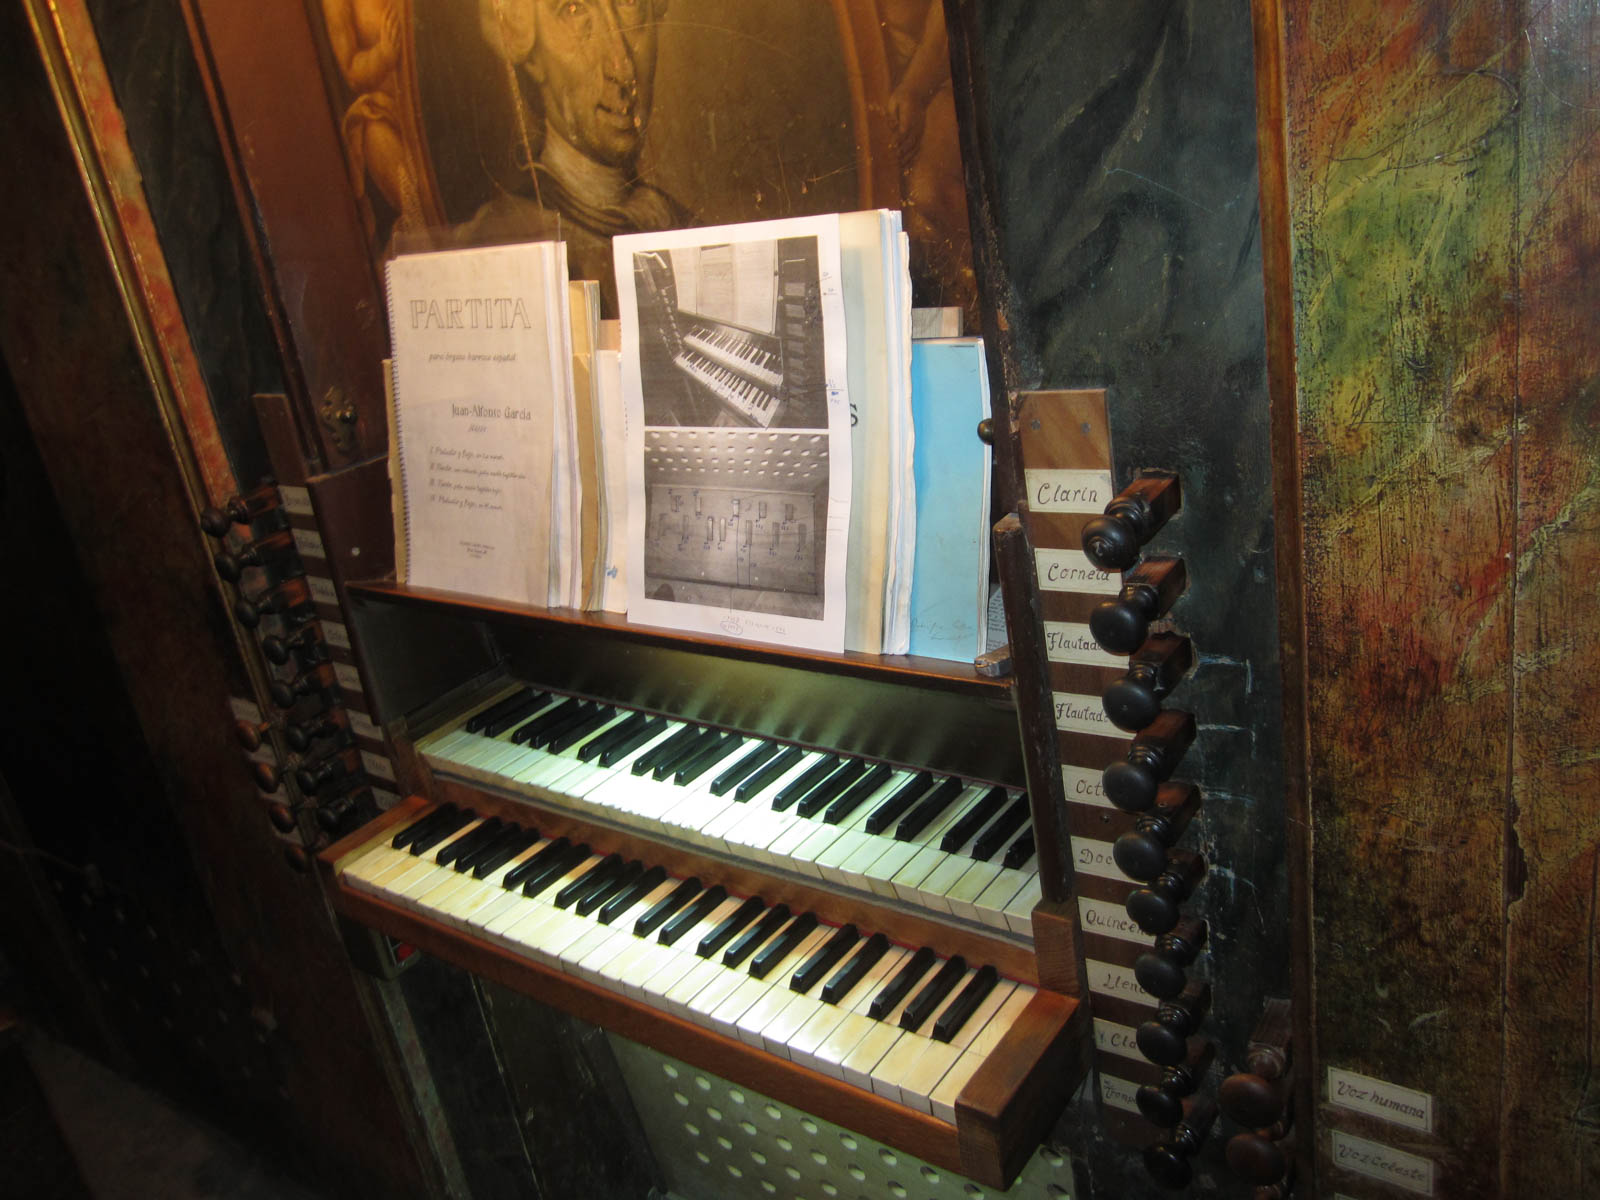
\includegraphics[width=\linewidth*3/4]{capitulo3/consola}
		\par\end{centering}
	\smallskip
	\caption{\label{fig:consola} Consola del órgano.}
\end{figure} 

\smallskip

Para funcionar, el órgano se alimenta de aire. Antiguamente se utilizaba un fuelle gigante, situado en la antesala, que llevaba el aire a una cámara de almacenamiento, para proporcionar un flujo de entrada constante. Esto requería que hubiese alguien follando mientras el organista tocaba. Hoy día el fuelle ha sido sustituído por una bomba eléctrica.

\smallskip

\begin{figure}[H]
	\noindent \begin{centering}
		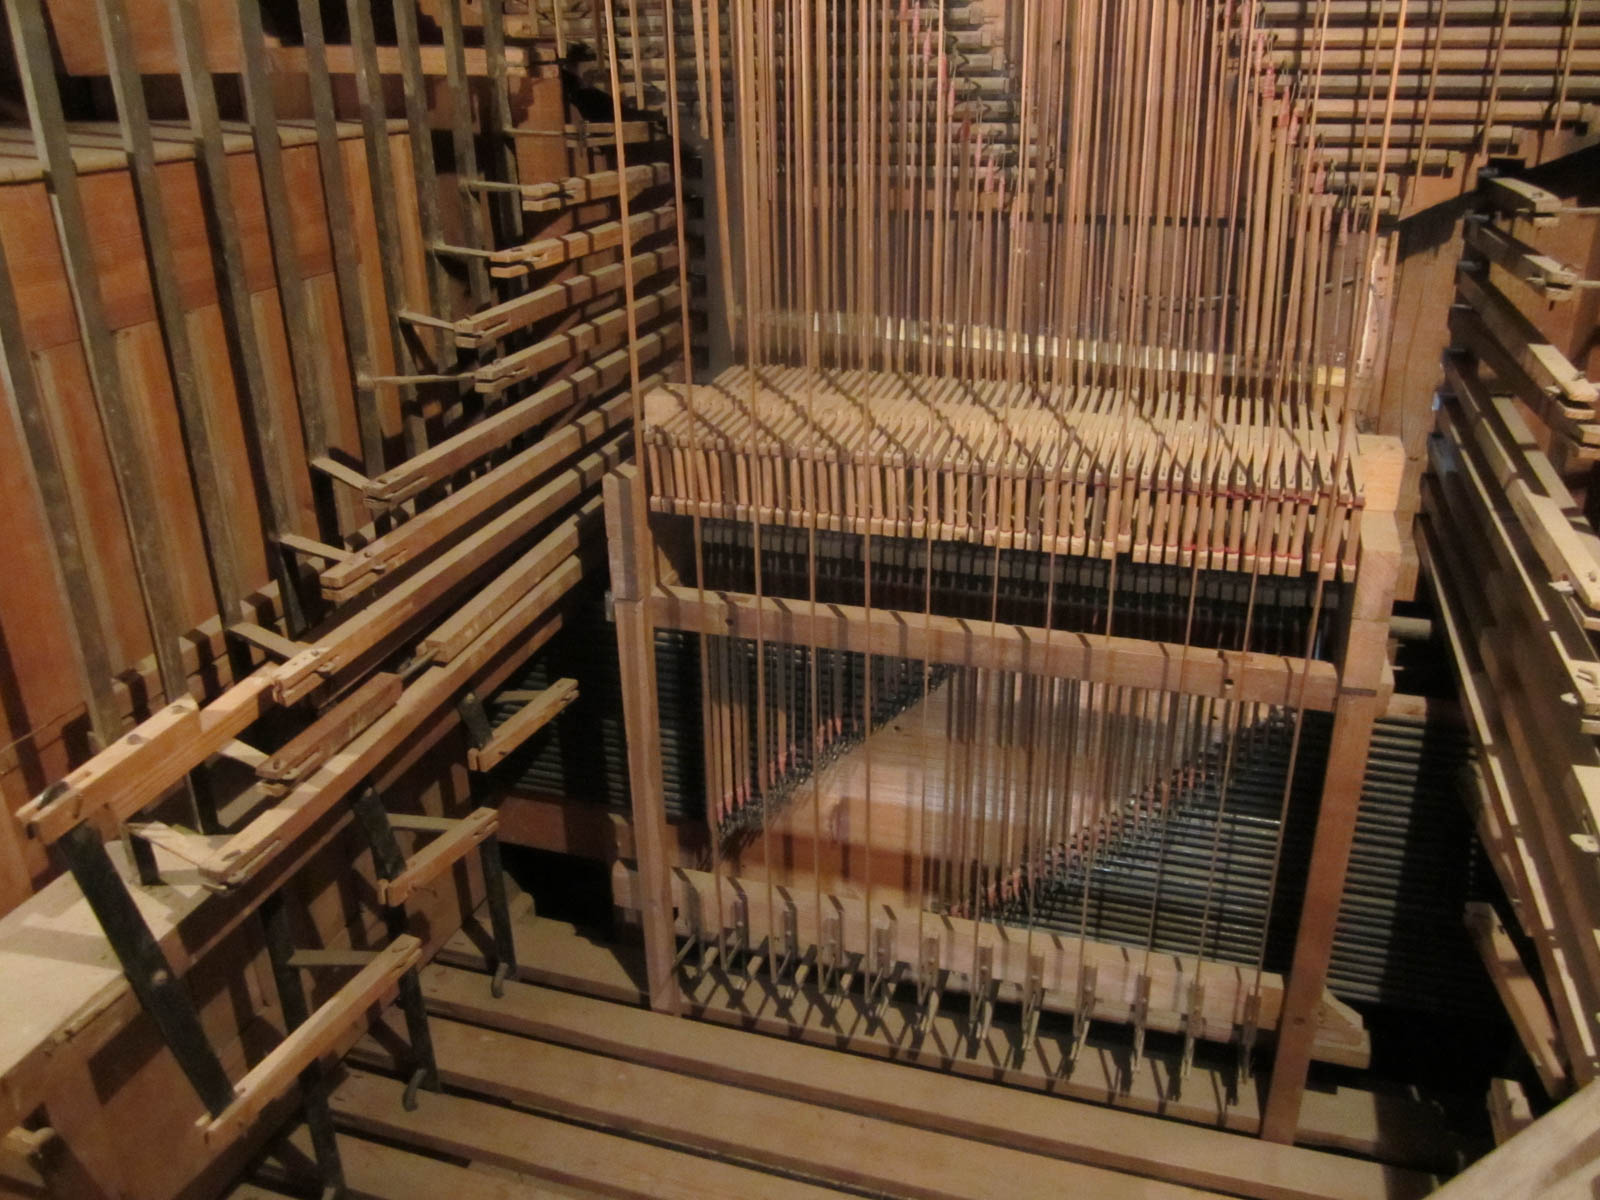
\includegraphics[width=\linewidth*3/4]{capitulo3/mecanismos}
		\par\end{centering}
	\smallskip
	\caption{\label{fig:mecanismos} Mecanismos detrás de la consola.}
\end{figure} 

\smallskip

Los entresijos del órgano barroco, el más grande, está construidos en dos plantas: en la parte más baja, a la altura de la consola, encontramos los juegos de palancas, de las cuales aquellas pertenecientes al órgano barroco suben a la planta superior. A sendos laterales encontramos el corazón del órgano romántico, más pequeño.

\smallskip

\begin{figure}[H]
	\noindent \begin{centering}
		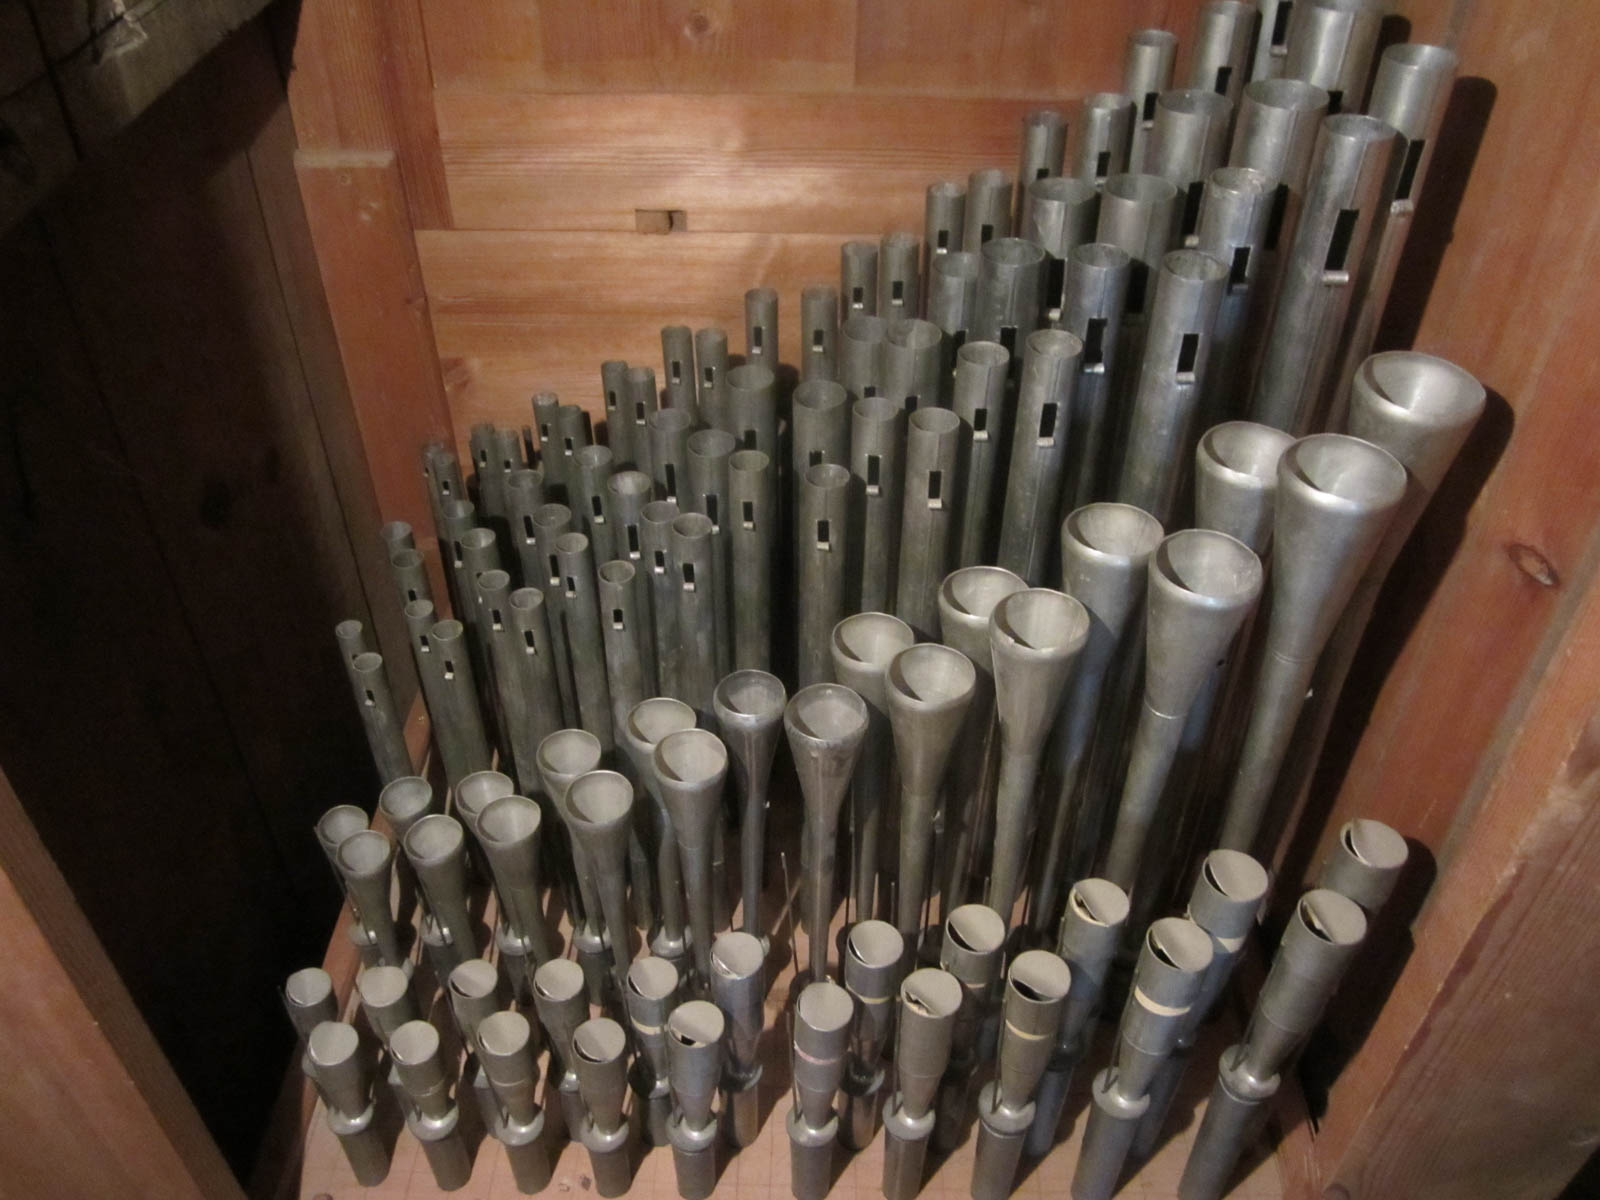
\includegraphics[width=\linewidth*2/3]{capitulo3/romantico}
		\par\end{centering}
	\smallskip
	\caption{\label{fig:romantico} Tubos del órgano romántico.}
\end{figure} 

\smallskip

En la planta de arriba se encuentra la esencia del instrumento: alrededor de 600 tubos de diferentes timbres y alturas sonoras, incluyendo el \textit{bajo de contrast}, que se hace sonar con el \textit{pedalier}. Solo los diapasones ---los flautados de 13' fundamentales y las cornetas--- son visibles desde el exterior.

\smallskip

\begin{figure}[H]
	\noindent \begin{centering}
		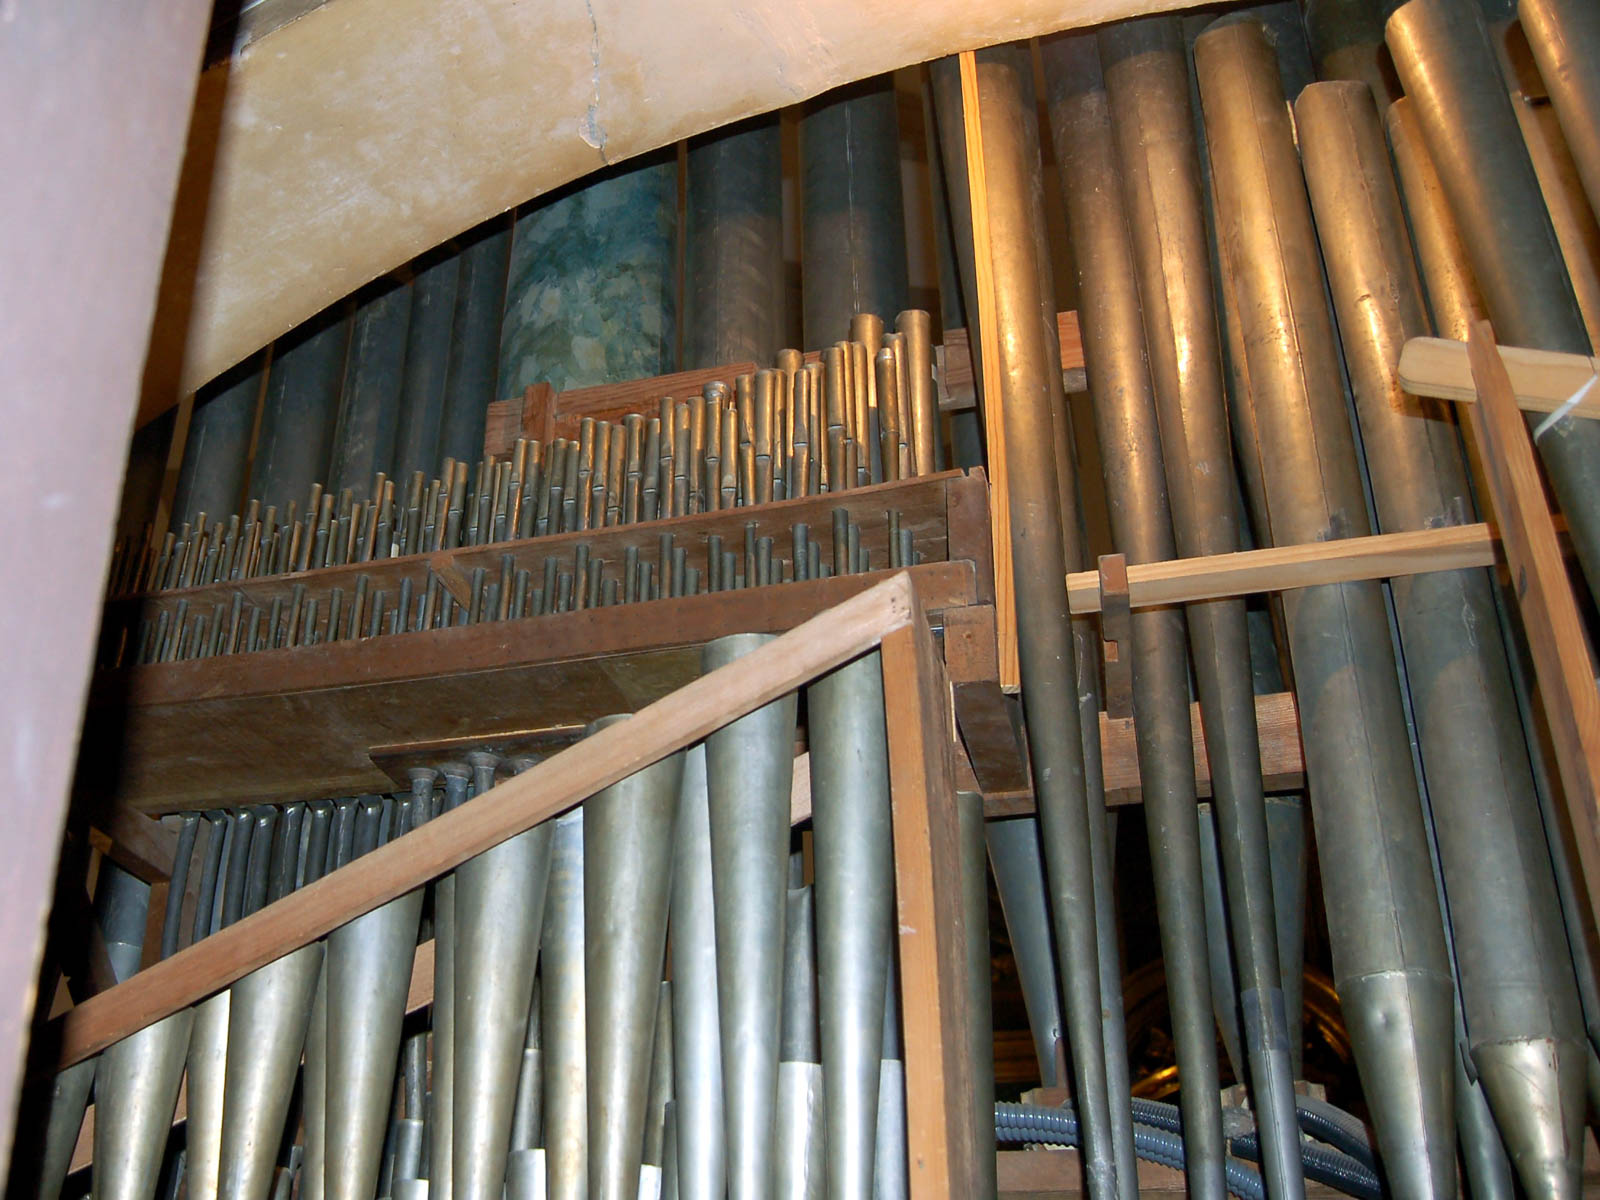
\includegraphics[width=\linewidth*2/3]{capitulo3/barroco}
		\par\end{centering}
	\smallskip
	\caption{\label{fig:barroco} Tubos del órgano barroco.}
\end{figure} 

\smallskip

La parte más importante del órgano es el llamado \textbf{secreto}, una galería a la que entra el aire procedente de la cámara de almacenamiento y se distribuye en cientos de conductos que llevan a las válvulas y los tubos. Siendo éste el corazón de la obra, dentro de él se halla una partitura firmada por el constructor del órgano. En tiempos en los que no existían los manguitos de goma, los conductos están tallados artesanalmente dentro de bloques de madera.

La primera tarea que llevamos a cabo fue conocer el órgano en profundidad, tomar algunas medidas y diseñar el modelo en 3D con el \textit{software} \textit{SolidWorks}.

\subsection{Teclados}

Tenemos dos teclados de cuatro octavas notas cada uno, el de arriba, correspondiente al órgano barroco, y otro más abajo, que sobresale del primero, para el órgano romántico, de la misma extensión.

\smallskip

\begin{figure}[H]
	\noindent \begin{centering}
		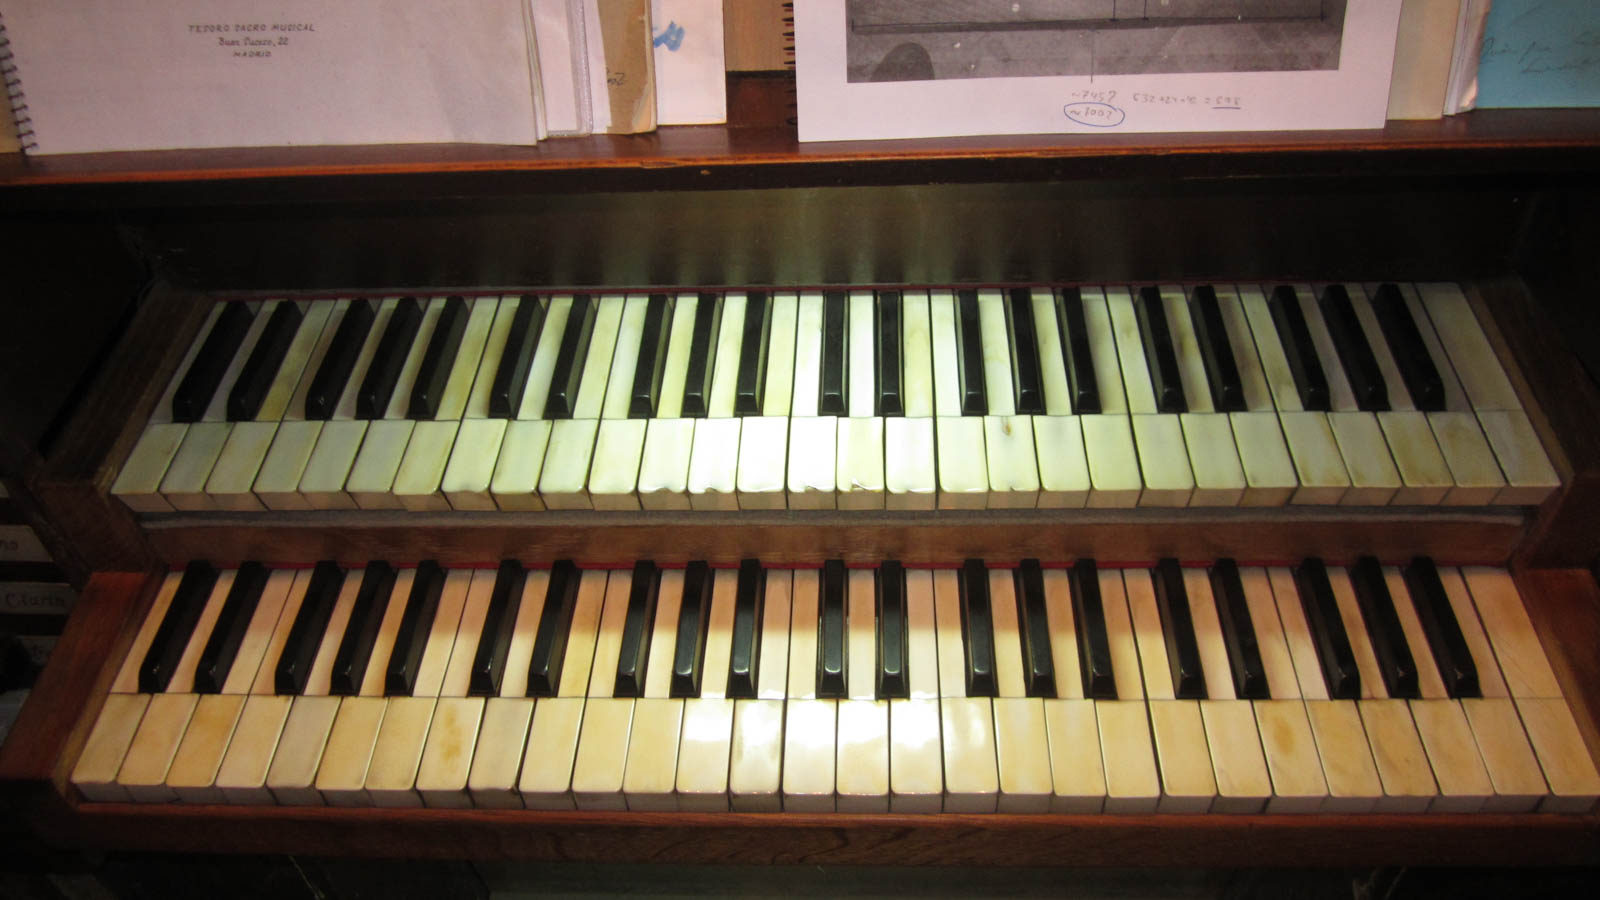
\includegraphics[width=\linewidth*3/4]{capitulo3/teclados}
		\par\end{centering}
	\smallskip
	\caption{\label{fig:teclados} Teclados del órgano.}
\end{figure} 

\smallskip

Tanto las medidas de cada tecla como su calado (diferencia entre la posición del borde de una tecla pulsada y sin pulsar) son estándar y coincidentes con las del piano. De la misma forma, la tecla \textit{Do} del centro hace sonar la nota \textit{Do 4} \footnotemark.

\footnotetext{En España se utilizan dos índices de notación musical: el franco-belga, que asigna el nombre \textit{La 3} a la nota cuya frecuencia fundamental vibra a 440 \textit{Hz}, y el índice científico, que asigna \textit{La 4} a la misma nota. En este proyecto utilizaremos el índice científico, ya que es el utilizado para el sistema \acrshort{MIDI}.}

Los datos más relevantes son los siguientes:

\smallskip

\begin{center}
	\begin{tabular}{|l|l|}
		\hline Número de teclas & 49 / teclado \\
		\hline Extensión & \textit{Do 2} -- \textit{Do 6} \\
		\hline Profundidad de calado (blancas) & 10 \textit{mm} \\
		\hline Profundidad de calado (negras) & 8 \textit{mm} \\
		\hline Presión máxima & 2,70 \textit{N} \\
		\hline
	\end{tabular}
	\smallskip
	\captionof{table}{\label{tab:teclados} Medidas de los teclados.}
\end{center}

\smallskip

Cada tecla blanca del mismo nombre tiene unas medidas ligeramente diferentes en su parte interna, para permitir que las negras encajen perfectamente. Las medidas de una tecla blanca son las siguientes:

\smallskip

\begin{figure}[H]
	\noindent \begin{centering}
		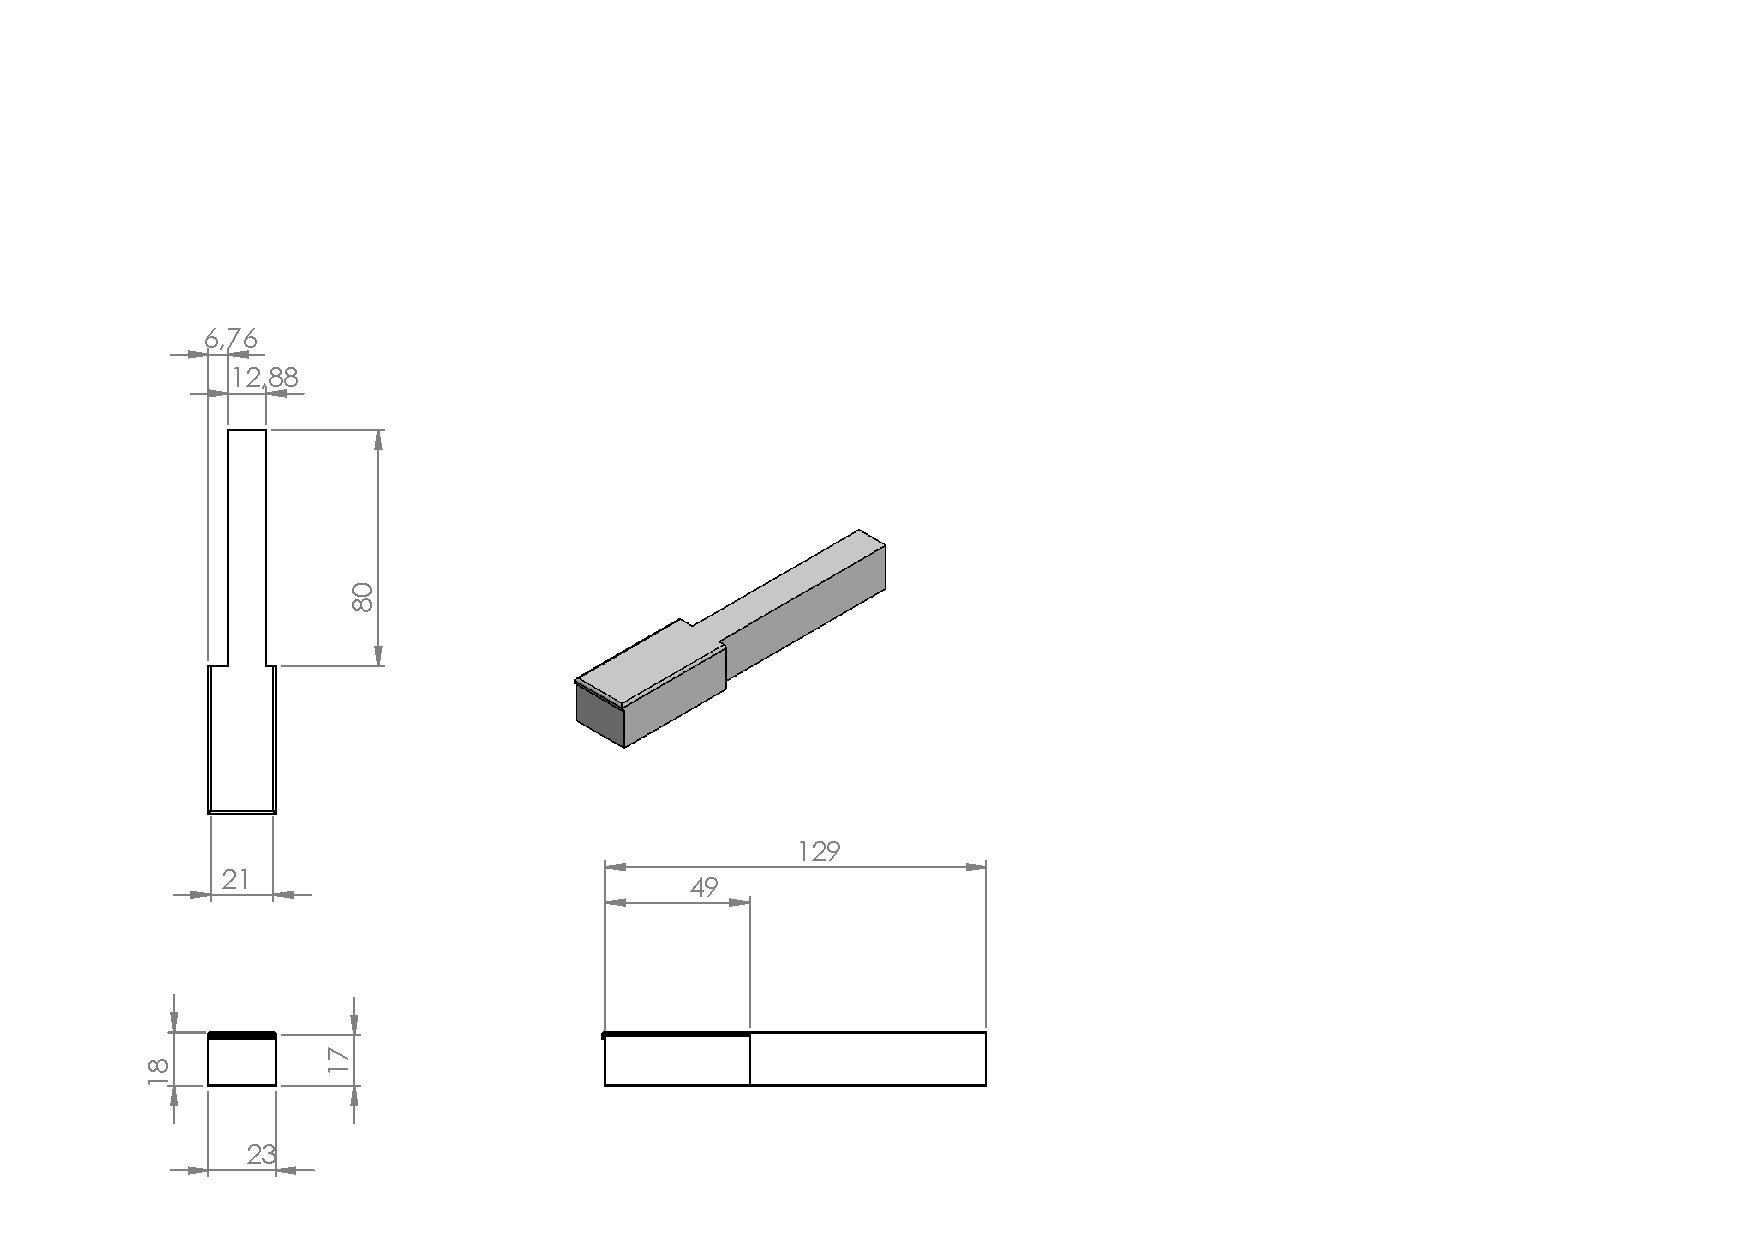
\includegraphics[clip=true,trim=0 0 360 150, width=\linewidth/2]{capitulo3/blanca_modelo}
		\par\end{centering}
	\smallskip
	\caption{\label{fig:blanca_modelo} Medidas de una tecla blanca.}
\end{figure} 

\smallskip

Las teclas negras, en cambio, son más cortas y más delgadas, sobresaliendo del teclado entre las blancas. Producen las notas cromáticas.

\smallskip

\begin{figure}[H]
	\noindent \begin{centering}
		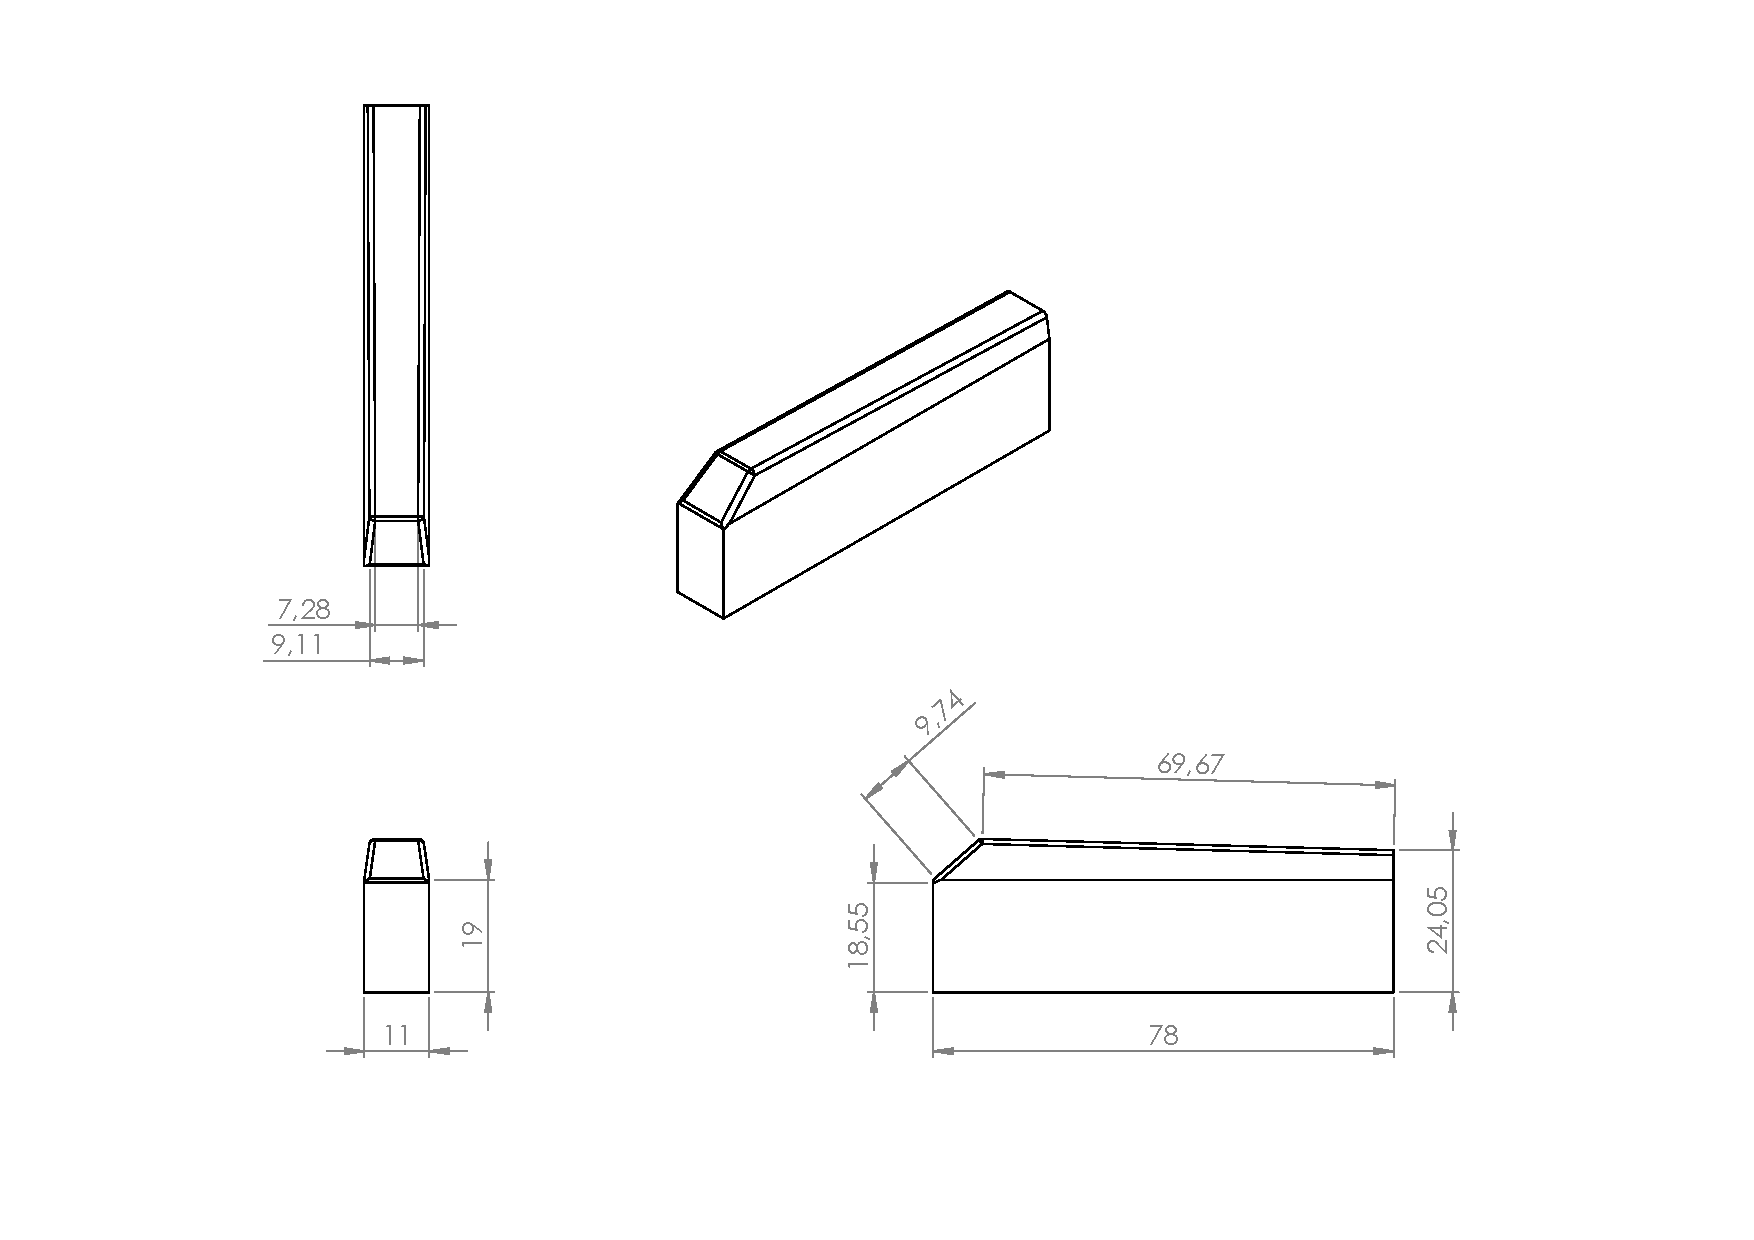
\includegraphics[clip=true,trim=50 50 50 50, width=\linewidth/2]{capitulo3/negra_modelo}
		\par\end{centering}
	\smallskip
	\caption{\label{fig:negra_modelo} Medidas de una tecla negra.}
\end{figure} 

\smallskip

A continuación presentamos las medidas tomadas sobre el teclado en conjunto:

\smallskip

\begin{figure}[H]
	\noindent \begin{centering}
		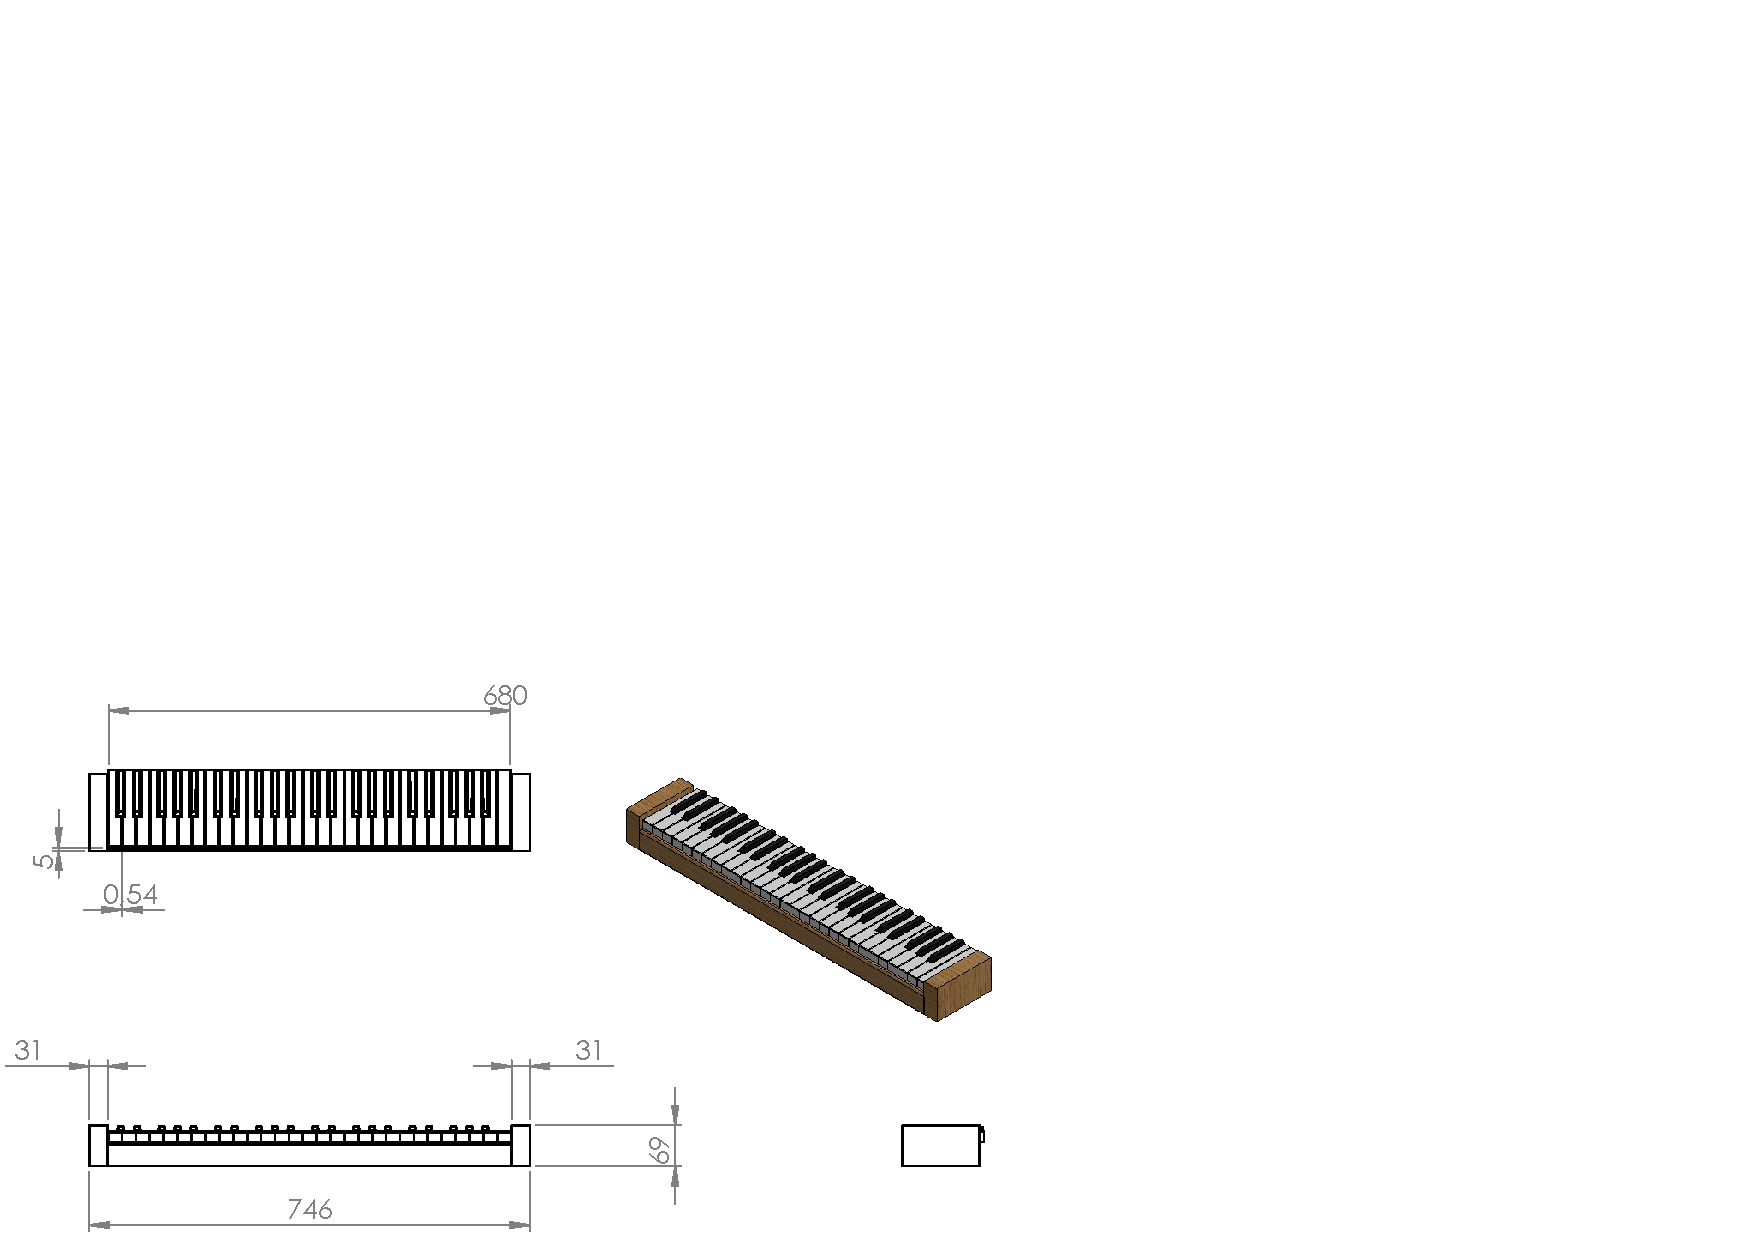
\includegraphics[clip=true,trim=0 0 360 320, width=\linewidth*3/4]{capitulo3/teclado_modelo}
		\par\end{centering}
	\smallskip
	\caption{\label{fig:teclado_modelo} Medidas del teclado.}
\end{figure} 

\smallskip

Cabe destacar que, a diferencia del piano, la intensidad del sonido no viene dada por la fuerza con la que se pulse una tecla, y no es necesario pulsarla hasta el tope de calado para que suene, basta con hacerla bajar tan solo unos milímetros, lo necesario para vencer la válvula.

\subsection{Pedales}

Este órgano cuenta con un \textit{pedalier} con un registro fijo: el \textit{bajo de contrast}. Los pedales están dispuestos en forma de escala diatónica, igual que las teclas. Cada pedal tiene aproximadamente la misma anchura que una tecla aunque, obviamente, están más separados unos de otros.

\smallskip

\begin{figure}[H]
	\noindent \begin{centering}
		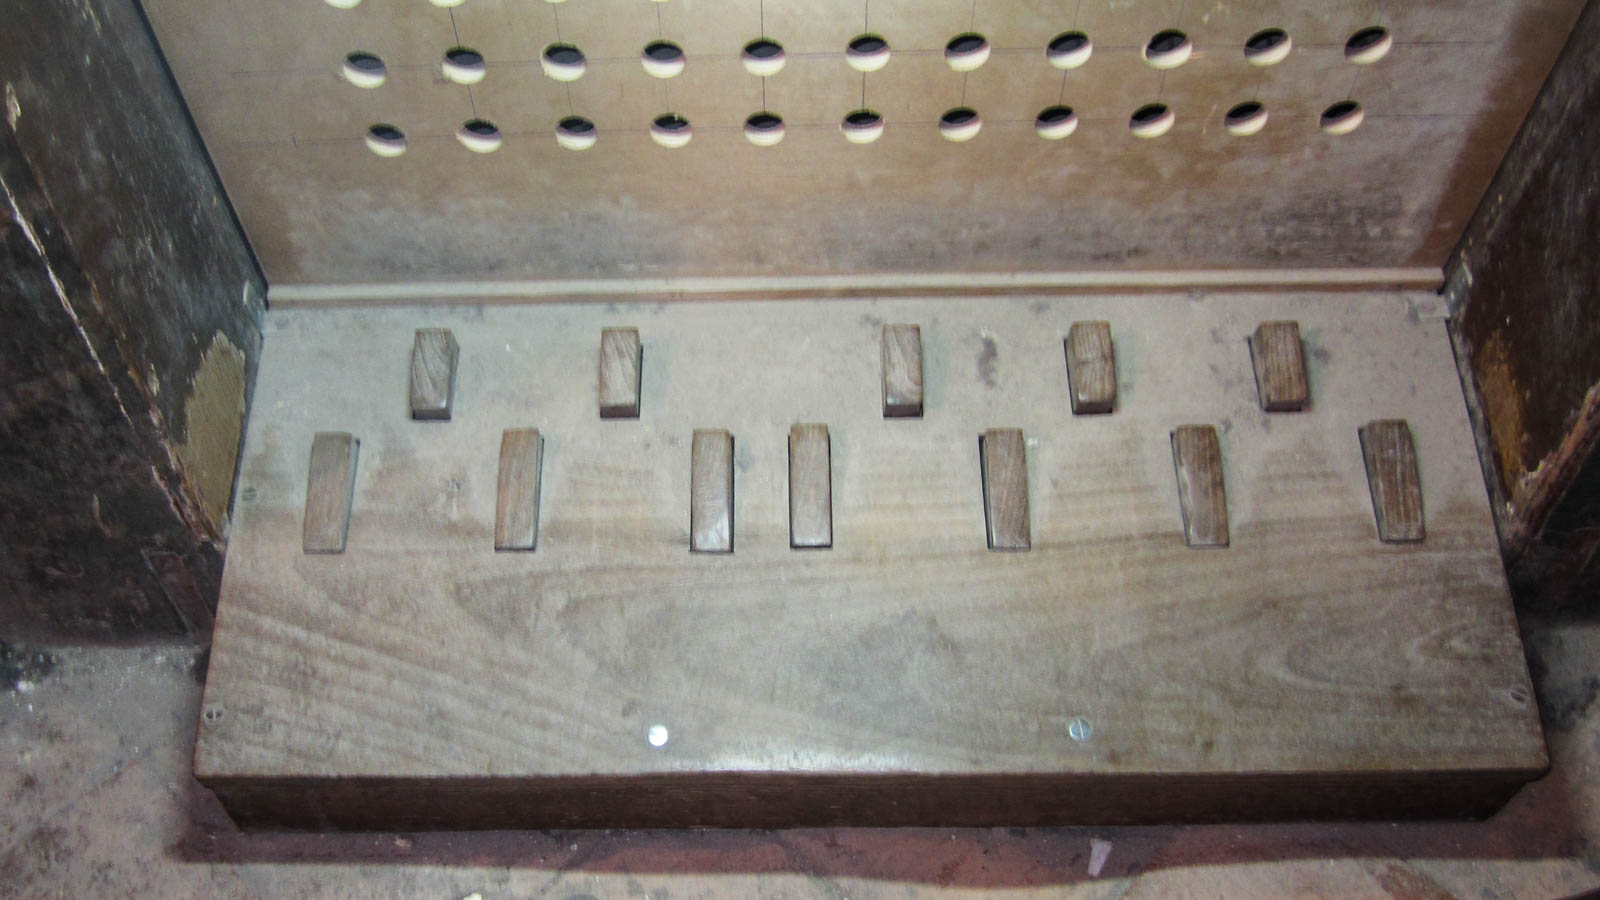
\includegraphics[width=\linewidth*3/4]{capitulo3/pedalier}
		\par\end{centering}
	\smallskip
	\caption{\label{fig:pedalier} \textit{Pedalier} del órgano.}
\end{figure} 

\smallskip

Es importante saber que el peso necesario para mover un pedal es mucho mayor que para una tecla, asimismo, tanto la naturaleza artesanal como el deterioro crean mucha disparidad entre el tacto de cada pedal.

\smallskip

\begin{center}
	\begin{tabular}{|l|l|}
		\hline Número de pedales & 12 \\ 
		\hline Extensión & \textit{Do 1} -- \textit{Si 1} \\ 
		\hline Profundidad de calado (diatónicas) & 14,5 \textit{mm} \\ 
		\hline Profundidad de calado (cromáticas) & 19,8 \textit{mm} \\
		\hline Presión máxima & 30,54 \textit{N} \\
		\hline 
	\end{tabular}
	\smallskip
	\captionof{table}{\label{tab:pedalier} Medidas del \textit{pedalier}.}
\end{center}

\smallskip

Por su parte, las cotas que definen el \textit{pedalier} son las siguientes:

\smallskip

\begin{figure}[H]
	\noindent \begin{centering}
		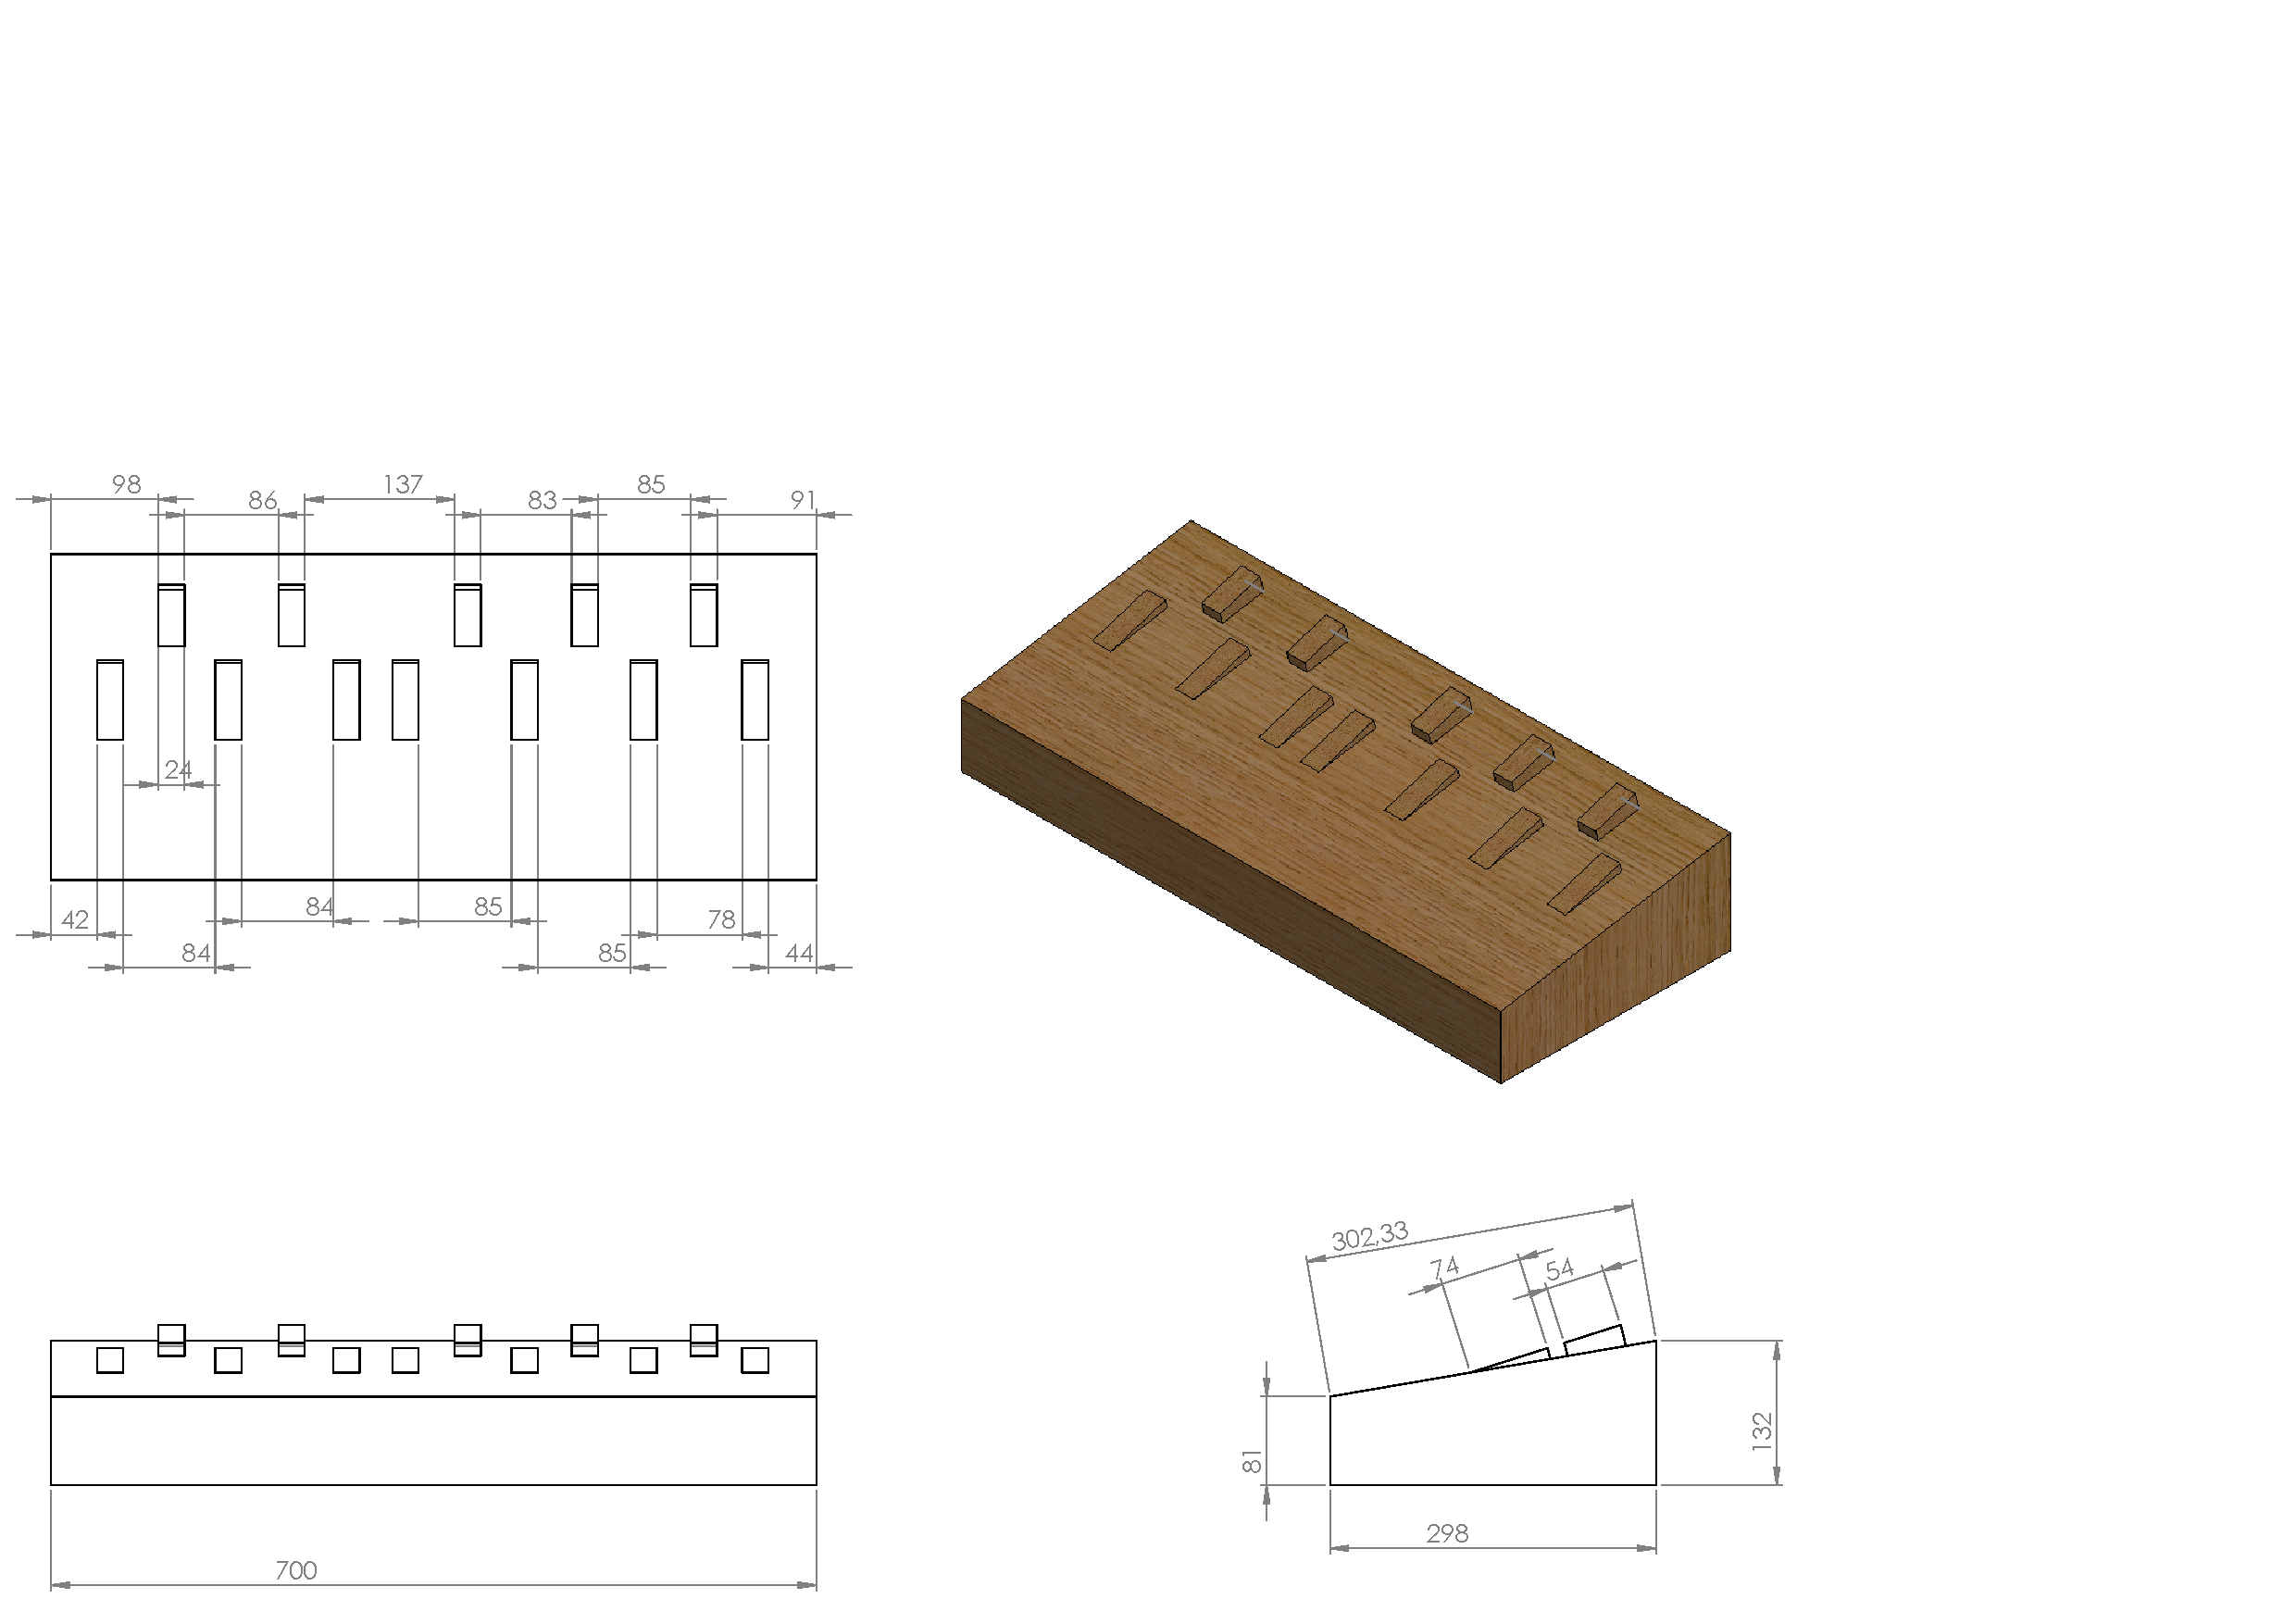
\includegraphics[clip=true,trim=0 0 260 250, width=\linewidth*3/4]{capitulo3/pedalier_modelo}
		\par\end{centering}
	\smallskip
	\caption{\label{fig:pedalier_modelo} Medidas de los pedales.}
\end{figure} 

\smallskip

\subsection{Registros}

Los registros son las diferentes familias de tubos con el mismo timbre y la misma tesitura. Se pueden abrir o cerrar desde la consola a través de una serie de palancas, de las que se tira para hacer sonar el registro o se empuja para silenciarlo.

\smallskip

\begin{figure}[H]
	\noindent \begin{centering}
		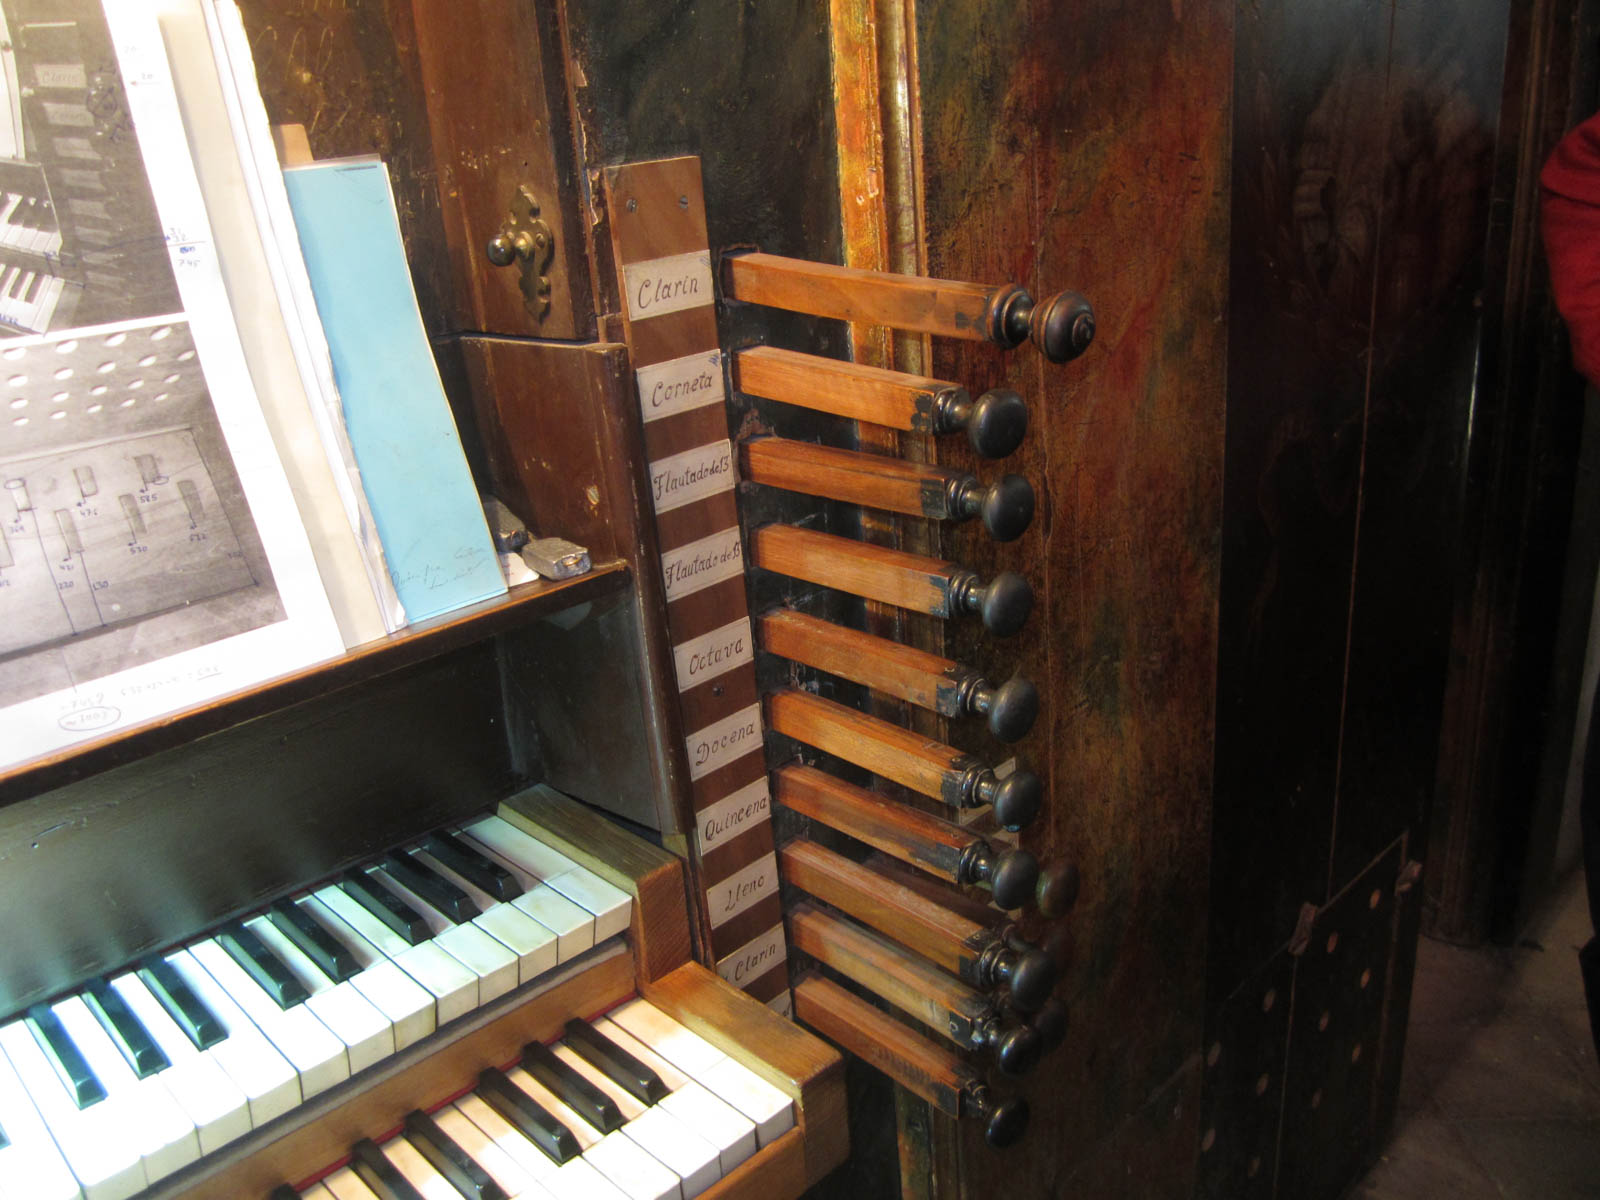
\includegraphics[width=\linewidth*2/3]{capitulo3/registros}
		\par\end{centering}
	\smallskip
	\caption{\label{fig:registros} Registros a la derecha del teclado.}
\end{figure} 

\smallskip

Estos controles están dispuestos a ambos lados de los teclados y son exclusivos para un teclado u otro. En este órgano existen registros parciales, esto es, se aplican solo a una mitad del teclado, bien de \textit{Do 2} a \textit{Si 3}, o bien de \textit{Do 4} a \textit{Do 6}.

Dado que el punto interno de equilibro de cada palanca está en lugares diferentes, existe una notable disparidad en la medida en que sobresalen cuando se abren. Además, tenemos una palanca especial, el \textit{tremolo}, que sirve para activar un mecanismo que produce un efecto de fluctuación en el sonido.

A continuación mostramos las medidas de longitud tomadas durante el análisis.

\smallskip

\begin{center}
	\begin{tabular}{|l|l|}
		\hline \multicolumn{2}{|c|}{\textbf{A la izquierda}} \\	
		\hline & Bajoncillo (142 \textit{mm}) \\ 
		\hline & Flautado de 13' sordina (160 \textit{mm}) \\ 
		\hline & Flautado de 13' (175 \textit{mm})\\ 
		\hline & Octava (161 \textit{mm}) \\ 
		\hline & Quincena (161 \textit{mm}) \\ 
		\hline Trémolo (67 \textit{mm}) & Decimonovena (165 \textit{mm}) \\ 
		\hline Bajón-oboe (103 \textit{mm}) & Lleno (140 \textit{mm})  \\ 
		\hline Flauta armenia (1106 \textit{mm}) & Clarín (160 \textit{mm}) \\ 
		\hline  Violón (100 \textit{mm}) & Trompeta real (144 \textit{mm})  \\ 
		\hline
	\end{tabular}
	\smallskip
	\captionof{table}{\label{tab:registros_izquierda} Medidas de los registros (izquierda).}
\end{center}

\smallskip
	
\begin{center}
	\begin{tabular}{|l|l|}
		\hline \multicolumn{2}{|c|}{\textbf{A la derecha}} \\
		\hline Clarín (170 \textit{mm}) &  \\ 
		\hline Corneta (141 \textit{mm}) &  \\ 
		\hline Flautado de 13' sordina (137 \textit{mm}) &  \\ 
		\hline Flautado de 13' (134 \textit{mm}) &  \\ 
		\hline Octava & (142 \textit{mm}) \\ 
		\hline Docena & (142 \textit{mm}) \\ 
		\hline Quincena & (168 \textit{mm}) \\ 
		\hline Lleno (156 \textit{mm}) & Voz humana (110 \textit{mm}) \\ 
		\hline Clarín (142 \textit{mm}) & Voz celeste (116 \textit{mm}) \\ 
		\hline Trompeta real (135 \textit{mm}) & Gamba (102 \textit{mm}) \\ 
		\hline 
	\end{tabular}
	\smallskip
	\captionof{table}{\label{tab:registros_derecha} Medidas de los registros (derecha).}
\end{center}

\smallskip

\section{PCB de control}

La placa de circuito impreso es la solución a los requisitos \textit{hardware} aportada por el proyecto de D. Mikel Aguayo Fernández \cite{mikel}. Incluye una serie de registros de desplazamiento para almacenar el estado del órgano, una interfaz de control local reducido y un medio de control remoto. También alimentará al computador que vamos a utilizar. Actualmente disponemos de un prototipo de la placa con un número limitado de salidas.

Una de las partes más importantes de este proyecto será desarrollar el \textit{software} controlador para esta \acrshort{PCB}. A continuación detallamos aquellos componentes con los que tendremos que interactuar.

\subsection{Registros de desplazamiento SN74HC595}

Los registros de desplazamiento son circuitos lógicos que almacenan una serie de bits y permiten desplazarlos de una celda a otra. Este modelo tiene una capacidad de 8 bits, soporta entrada en serie y salida en paralelo con registro de almacenamiento \cite{shiftreg}. 

Así, solo necesitamos un pin para enviar toda la información, y la salida no se ve alterada durante el desplazamiento, sino que damos un pulso de reloj para indicar que hemos terminado de enviar los datos.

\smallskip

\begin{figure}[H]
	\noindent \begin{centering}
		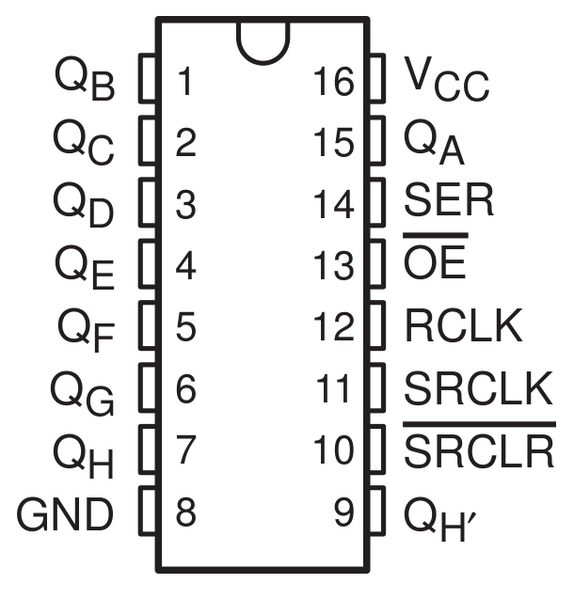
\includegraphics[width=\linewidth/4]{capitulo3/SN74HC595}
		\par\end{centering}
	\smallskip
	\caption{\label{fig:SN74HC595} Pines del SN74HC595. }
\end{figure} 

\smallskip

La información más relevante es la siguiente:

\smallskip

\begin{center}
		\begin{tabular}{|l|l|}
		\hline Capacidad & 8 \textit{bits} / canal \\ 
		\hline Canales & 4 \\ 
		\hline Ancho de pulso & 100 ns \\ 
		\hline 
	\end{tabular}
	\smallskip
	\captionof{table}{\label{tab:info_regdespl} Características de los registros de desplazamiento.}
\end{center}

\smallskip

Basándonos en el órgano de la Parroquia de Santa Fe, tendremos cuatro registros de desplazamiento, uno para cada canal:

\begin{itemize}
	\item Canal 1: teclado barroco.
	\item Canal 2: teclado romántico.
	\item Canal 3: registros.
	\item Canal 4: pedalier.
\end{itemize}

A pesar de que la capacidad de cada canal es de 8 bits, solo utilizaremos 7 de ellos.

\subsection{Conexión a la mecánica}

Los registros de desplazamiento están diseñados para albergar el estado lógico de cada una de las piezas del órgano con las que vamos a interactuar, y se han dispuesto cuidadosamente para que, clasificados por canales, cada uno se dedique a una zona de la consola del instrumento, manteniendo una interfaz lógica similar con objeto de homogeneizar la interfaz de cara al \textit{software}.

\subsubsection{Teclados}

Los dos primeros canales de control están asignados a los teclados. Un \textit{driver} de potencia interno aumentará la tensión a la salida de cada registro para llevarlo a la mecánica que pulsará las teclas. La siguiente figura ilustra este funcionamiento:

\smallskip

\begin{figure}[H]
	\noindent \begin{centering}
		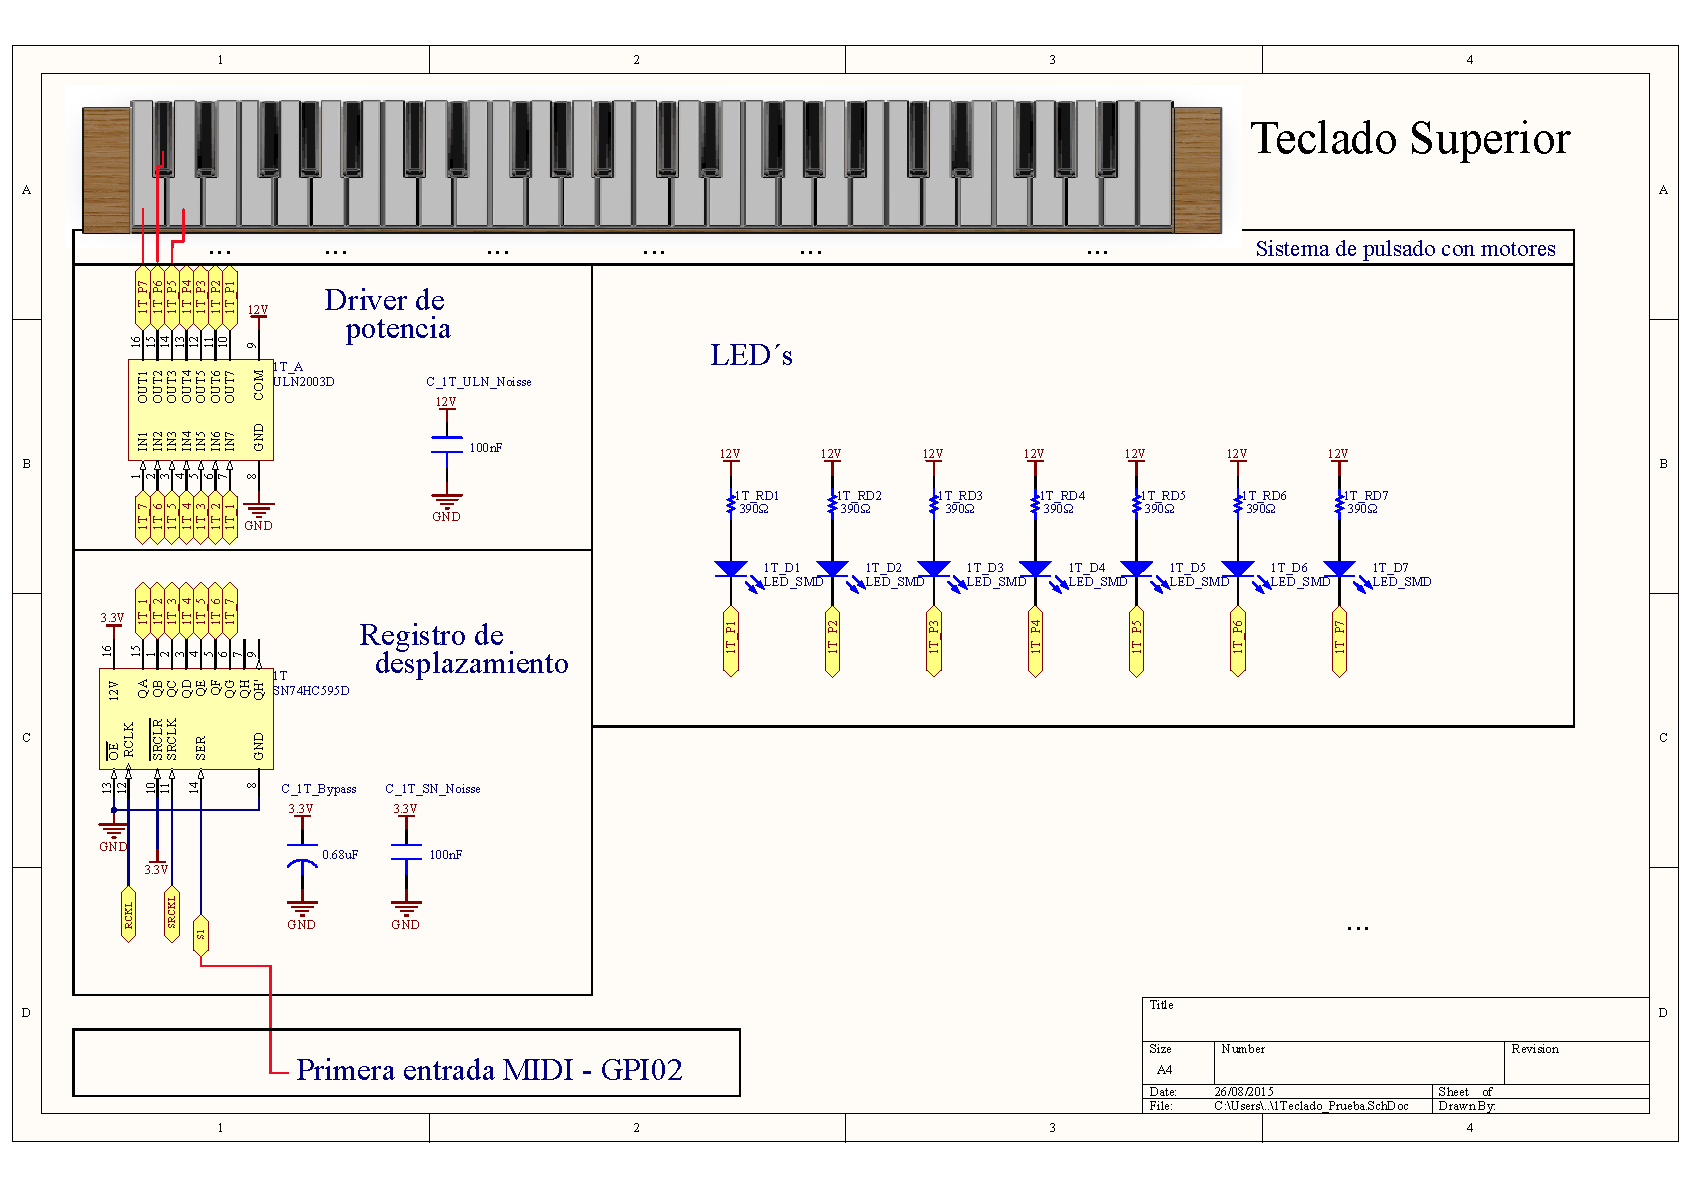
\includegraphics[width=\linewidth*2/3]{capitulo3/pcb_teclado}
		\par\end{centering}
	\smallskip
	\caption{\label{fig:pcb_teclado} Interfaz entre la \acrshort{PCB} y el teclado barroco.}
\end{figure} 

\smallskip

Los dos teclados se comportan de la misma forma, aunque al de abajo le corresponderá un canal diferente.

\subsubsection{Pedalier}

El \textit{pedalier} representa una escala musical, con los pedales bajos similares a las teclas blancas, diatónicas, mientras que los pedales altos emulan a las teclas negras, cromáticas. Por tanto, el esquema de funcionamiento es similar al de los teclados, aunque con menos extensión.

\smallskip

\begin{figure}[H]
	\noindent \begin{centering}
		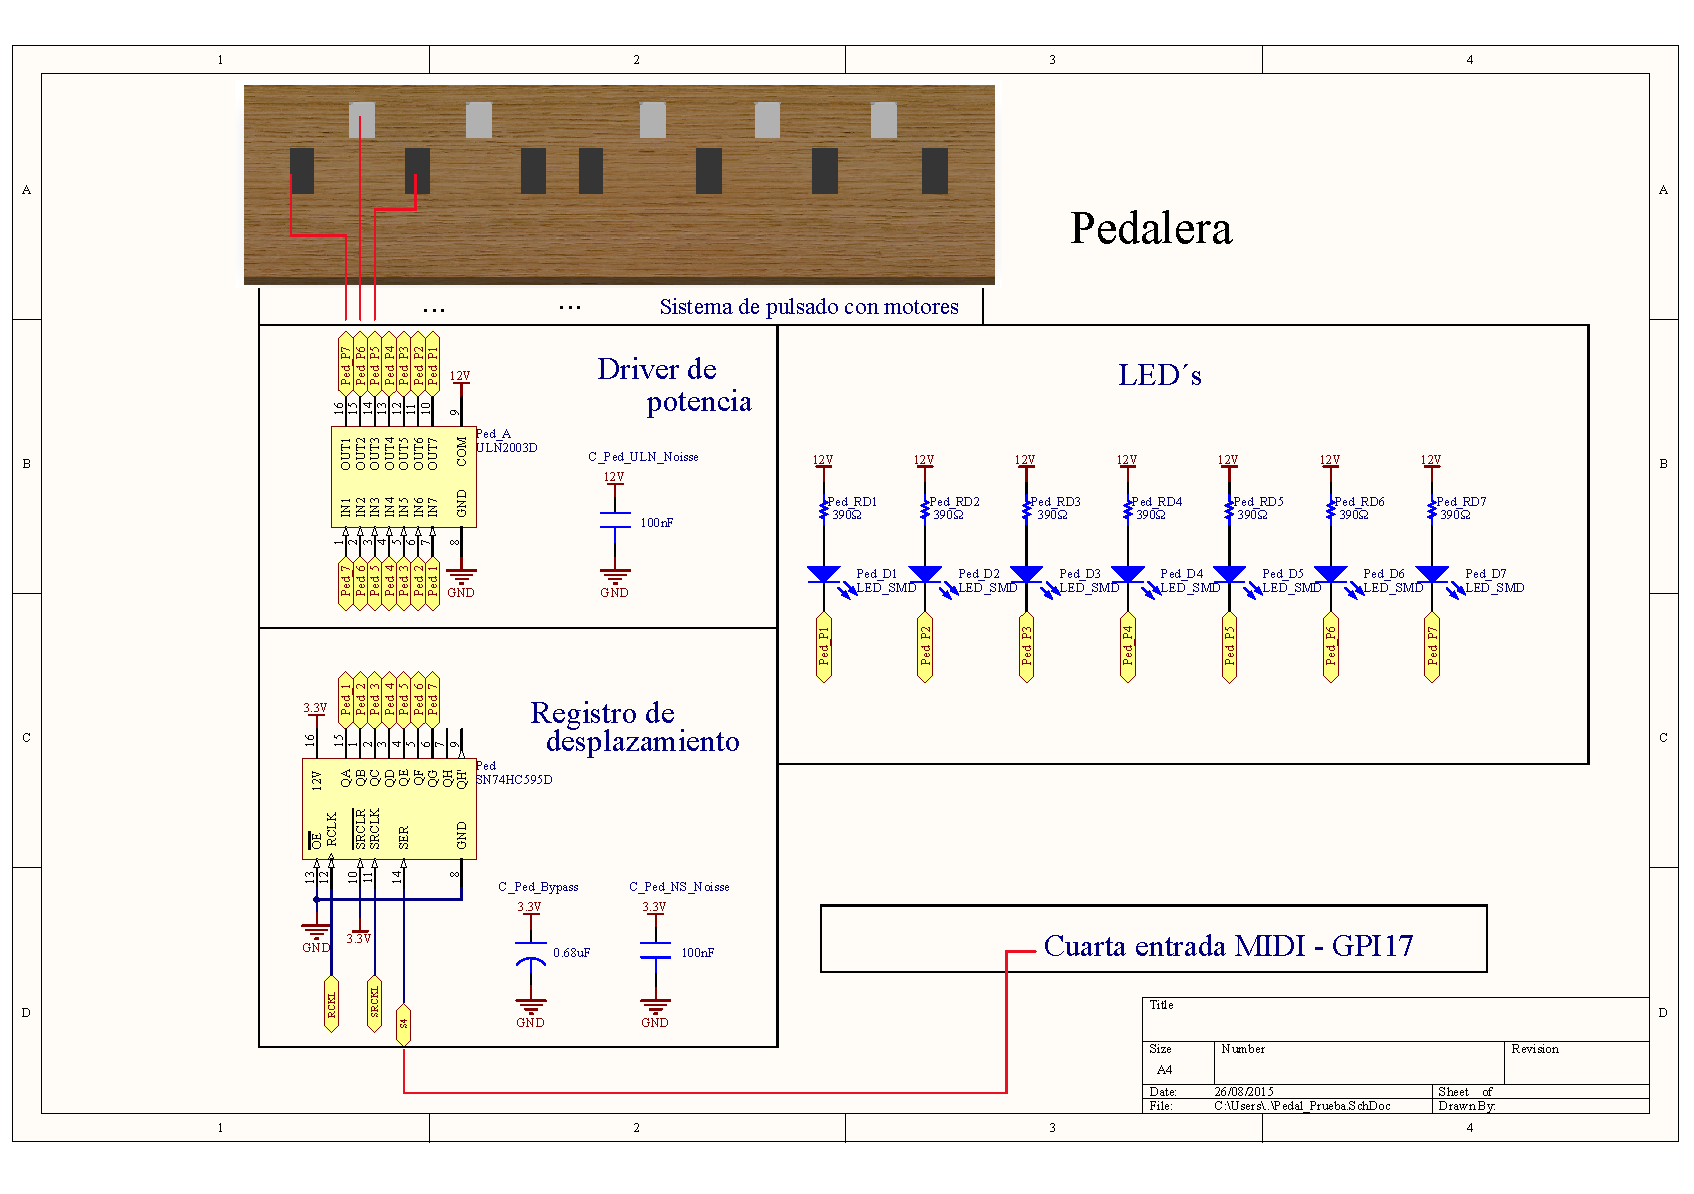
\includegraphics[width=\linewidth*2/3]{capitulo3/pcb_pedalier}
		\par\end{centering}
	\smallskip
	\caption{\label{fig:pcb_pedalier} Interfaz entre la PCB y el pedalier.}
\end{figure} 

\smallskip

\subsubsection{Registros de timbres}

Como podemos ver, los registros no se corresponden con teclas musicales y no tienen el mismo significado. Sin embargo, sí que tienen la misma estructura lógica, al contemplarse dos posiciones: abierto (hacia afuera) y cerrado (hacia dentro).

La mecánica a utilizar será diferente y, probablemente, algo más compleja, pero la interfaz para manejarlos se asemejará a del resto de controles:

\smallskip

\begin{figure}[H]
	\noindent \begin{centering}
		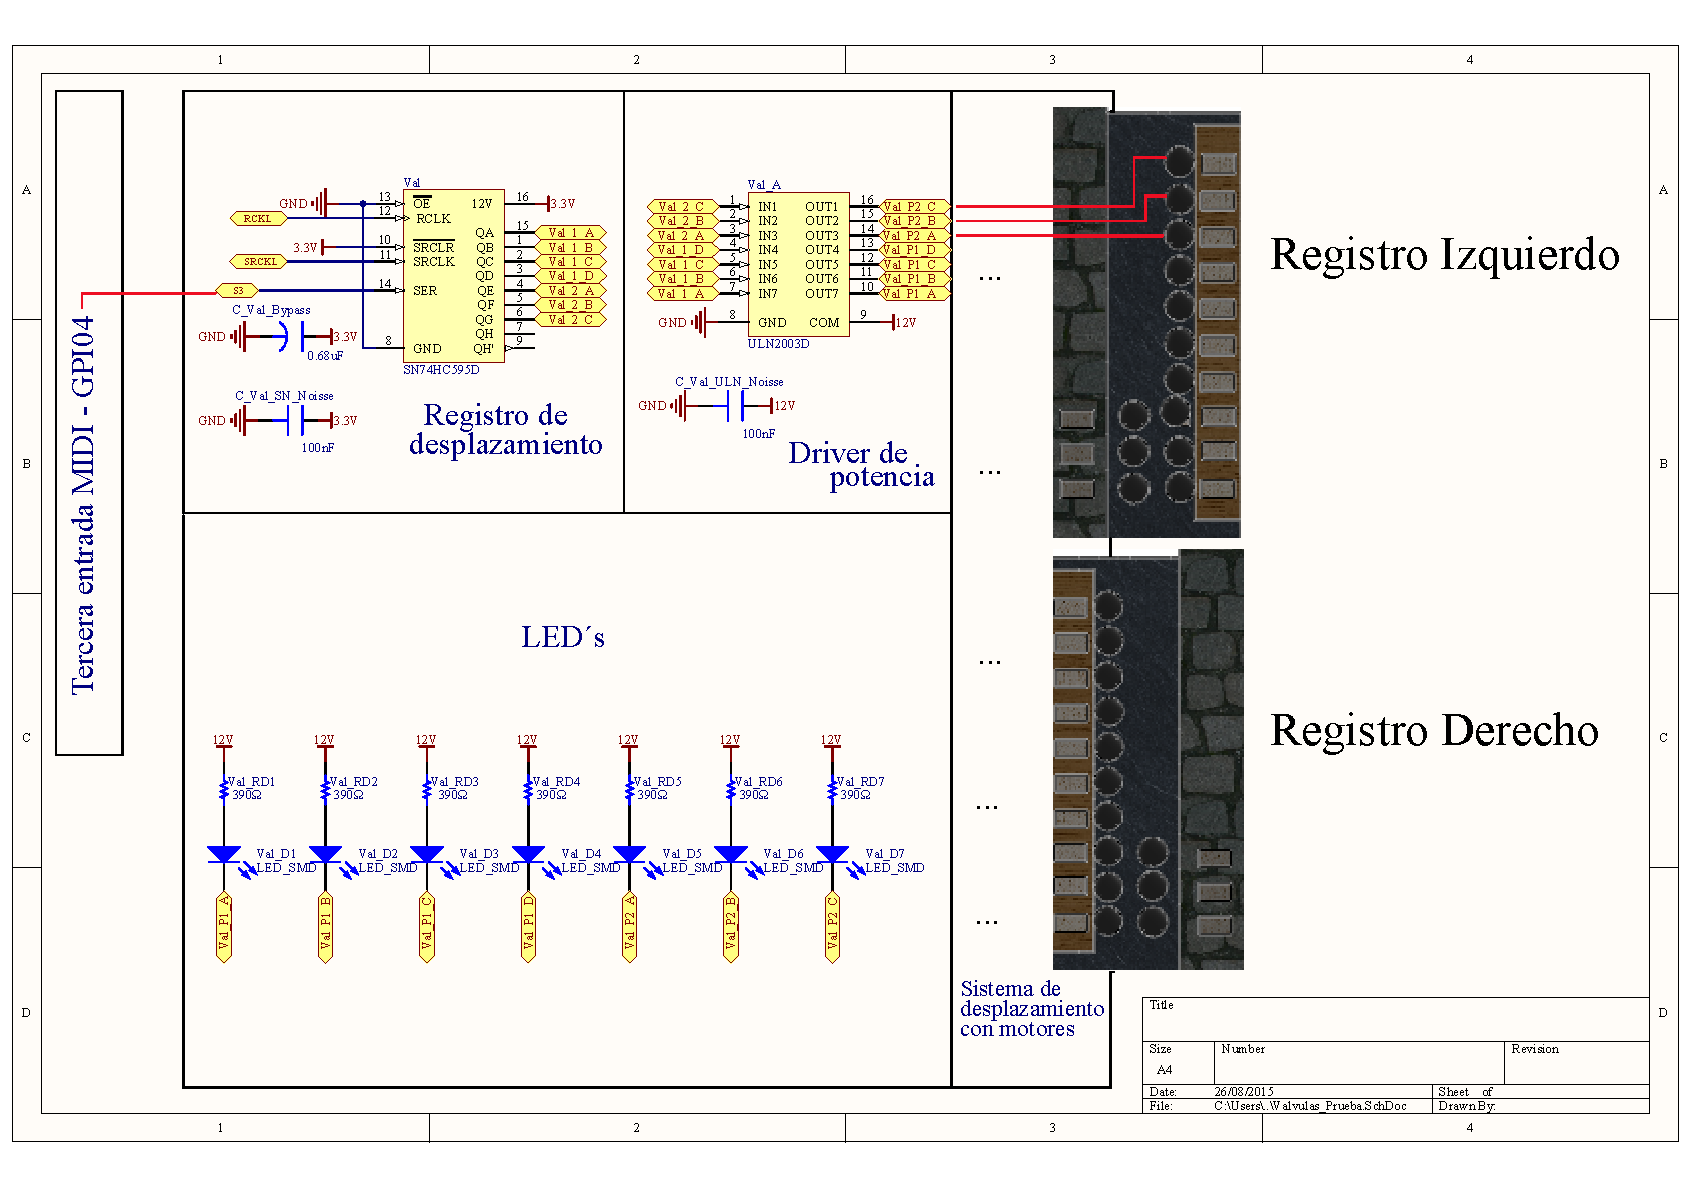
\includegraphics[width=\linewidth*2/3]{capitulo3/pcb_registros}
		\par\end{centering}
	\smallskip
	\caption{\label{fig:pcb_registros} Interfaz entre la PCB y las palancas de registros.}
\end{figure} 

\smallskip

\subsection{Receptor de mando a distancia HIRK-433A}

El receptor de mando a distancia es un detector de radio con decodificador a interfaz RS-232. Nos da la información del número de serie del mando y qué botones han disparado el evento. 

\smallskip

\begin{figure}[H]
	\noindent \begin{centering}
		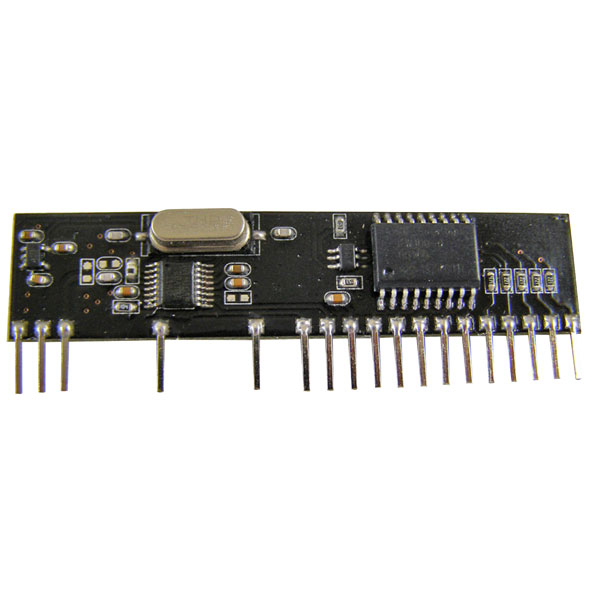
\includegraphics[clip=true,trim=0 200 0 200, width=\linewidth/2]{capitulo3/HIRK-433A}
		\par\end{centering}
	\smallskip
	\caption[Receptor de radio HIRK-433A.]{\label{fig:HIRK-433A} Receptor de radio HIRK-433A. \cite{imagen_decoder}}
\end{figure} 

\smallskip

Es flexible para mandos con distinto número de botones y los indica como un campo de bits basados en la letra A. Si el carácter corresponde a una minúscula, nos avisa de que el mando tiene poca batería. Por ejemplo:

\begin{itemize}
	\item \textbf{A}: Botón 1.
	\item \textbf{B}: Botón 2.
	\item \textbf{C}: Botones 1 y 2.
	\item \textbf{d}: Botón 3 (batería baja).
	\item \textbf{H}: Botón 4.
\end{itemize}

La siguiente tabla muestra los datos de nuestro interés:

\smallskip

\begin{center}
	\begin{tabular}{|l|l|}
		\hline Interfaz & RS-232 \\
		\hline Velocidad & 9600 \textit{baudios} \\ 
		\hline Longitud de trama & 10 \textit{bytes} \\ 
		\hline Sintaxis & <Nº serie (7 \textit{bytes})> <Botón (1 \textit{byte})> <CRLF> \\ 
		\hline 
	\end{tabular}
	\smallskip
	\captionof{table}[Características del receptor de mando.]{\label{tab:info_recv} Características del receptor de mando. \cite{datasheet_decoder}}
\end{center}

\smallskip

\subsection{Pantalla LCD FDCC2004B}

Esta pantalla es un \acrshort{LCD} (\textit{\acrlong{LCD}}) genérico basado en el Hitachi HD44780, considerado un estándar \textit{de facto} para este tipo de dispositivos. Tiene una pequeña memoria para almacenar el estado (no hay que enviar continuamente la información), tiene los caracteres \acrshort{ASCII} predefinidos y tiene capacidad para configurar hasta 8 caracteres especiales.

Esta pieza presenta el siguiente aspecto:

\smallskip

\begin{figure}[H]
	\noindent \begin{centering}
		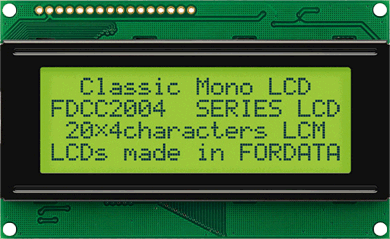
\includegraphics[width=\linewidth/2]{capitulo3/FDCC2004B}
		\par\end{centering}
	\smallskip
	\caption{\label{fig:FDCC2004B} LCD FDCC2004B.}
\end{figure} 

\smallskip

La siguiente tabla muestra sus características principales \cite{datasheet_lcd}:

\smallskip

\begin{center}
	\begin{tabular}{|l|l|}
		\hline Tipo & \acrshort{LCD} retroiluminado \\ 
		\hline Filas & 4 \\ 
		\hline Columnas & 20 \\ 
		\hline Dimensión de celda & 5 x 8 \textit{pixels} \\ 
		\hline Caracteres especiales & 8 \\ 
		\hline 
	\end{tabular}
	\smallskip
	\captionof{table}{\label{tab:info_lcd} Características de la pantalla LCD.}
\end{center} 

\smallskip

\subsection{Codificador rotatorio EC11J}

Un codificador rotatorio es un componente electrónico consistente en un botón giratorio, y emite una señal cuyas características dependen del sentido en que el usuario ha girado el botón. El modelo que vamos a utilizar contiene un botón giratorio y pulsable. \cite{rotary}

\smallskip

\begin{figure}[H]
	\noindent \begin{centering}
		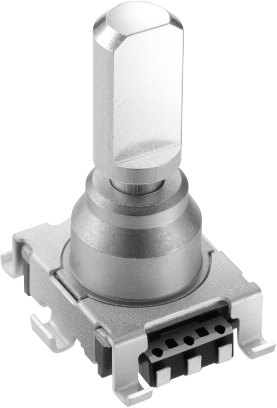
\includegraphics[width=\linewidth/4]{capitulo3/EC11J}
		\par\end{centering}
	\smallskip
	\caption{\label{fig:EC11J} Codificador rotatorio EC11J.}
\end{figure} 

\smallskip

La información nos viene dada por tres canales: uno para el pulsador y dos para la rotación. A medida que rotamos el botón, A y B oscilan produciendo una señal cuadrada que viene desfasada 90\textdegree, como la que aparece en la siguiente imagen:

\smallskip

\begin{figure}[H]
	\noindent \begin{centering}
		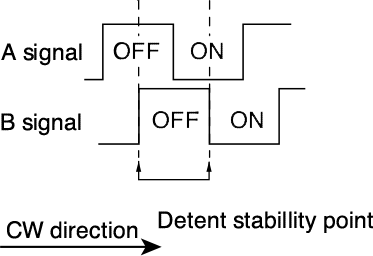
\includegraphics[width=\linewidth/3]{capitulo3/rotary}
		\par\end{centering}
	\smallskip
	\caption{\label{fig:rotary} Código de señales utilizado por el ECJ11.}
\end{figure} 

\smallskip

Los puntos de equilibro ---\textit{detent stability points}--- coinciden con los saltos del canal B, de forma que a la mitad del recorrido de un giro cambiará el canal A. Todo lo que tenemos que hacer entonces es detectar un cambio en A y comparar el valor de A y B: si son iguales, significa que se ha rotado en sentido antihorario; si son distintos, entendemos que se ha girado en sentido horario.

\subsection{Conexión entre la PCB y los periféricos}

\smallskip

\begin{figure}[H]
	\noindent \begin{centering}
		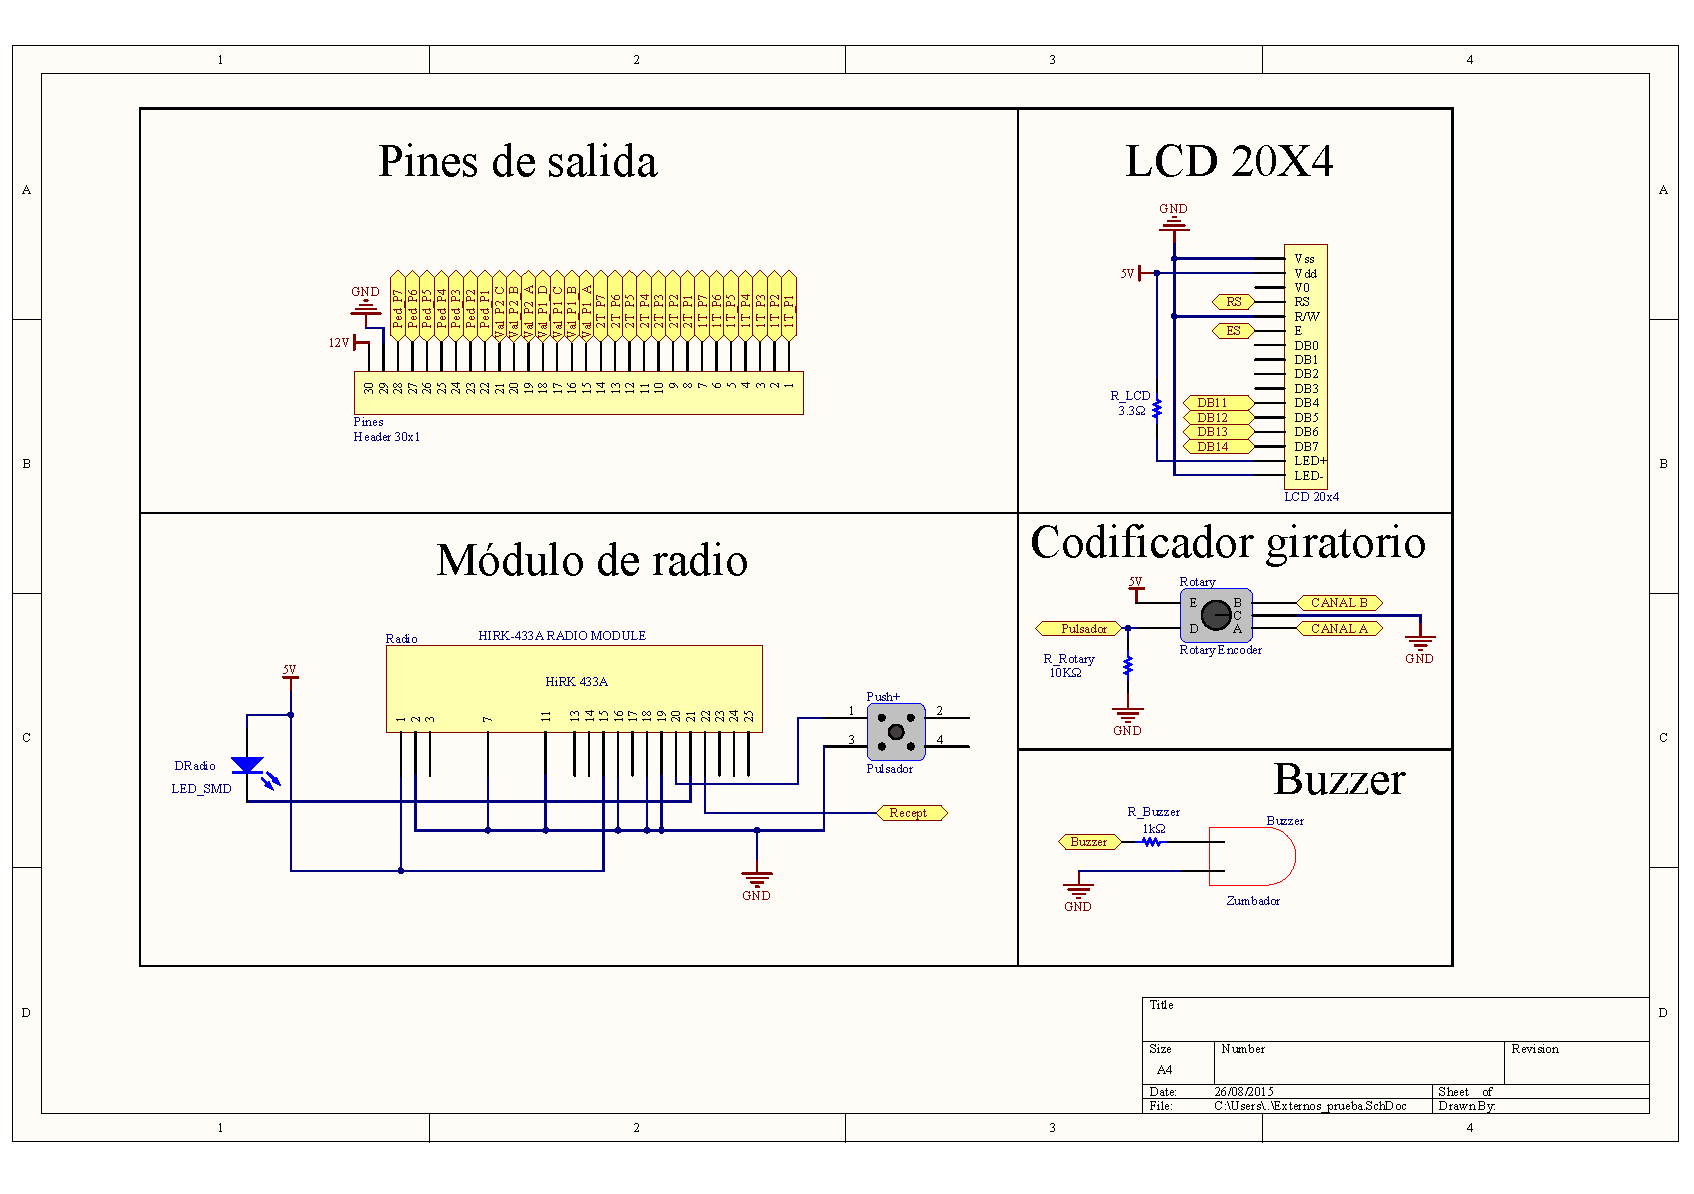
\includegraphics[width=\linewidth*2/3]{capitulo3/pcb_perifericos}
		\par\end{centering}
	\smallskip
	\caption{\label{fig:pcb_perifericos} Interfaz entre la PCB y los periféricos.}
\end{figure} 

\smallskip

\section{SBC Rasberry Pi}

El \textit{Raspberry Pi} es un ordenador de placa única ---\acrshort{PCB} (\textit{\acrlong{SBC}})---, más potente que un microcontrolador y con sistema operativo basado en Linux. Se alimenta por \textit{USB} y se puede controlar con teclado y ratón, o bien desde red mediante \acrshort{SSH}. 

El corazón de este computador es un \acrshort{SOCA} (\textit{\acrlong{SOCA}}), que integra microprocesador, memoria y periféricos principales. El modelo escogido, \textit{B+}, posee numerosos pines de entrada y salida de propósito general (\acrshort{GPIO}), que utilizaremos para interactuar con la \acrshort{PCB} y para ser alimentado por ésta.

\smallskip

\begin{figure}[H]
	\noindent \begin{centering}
		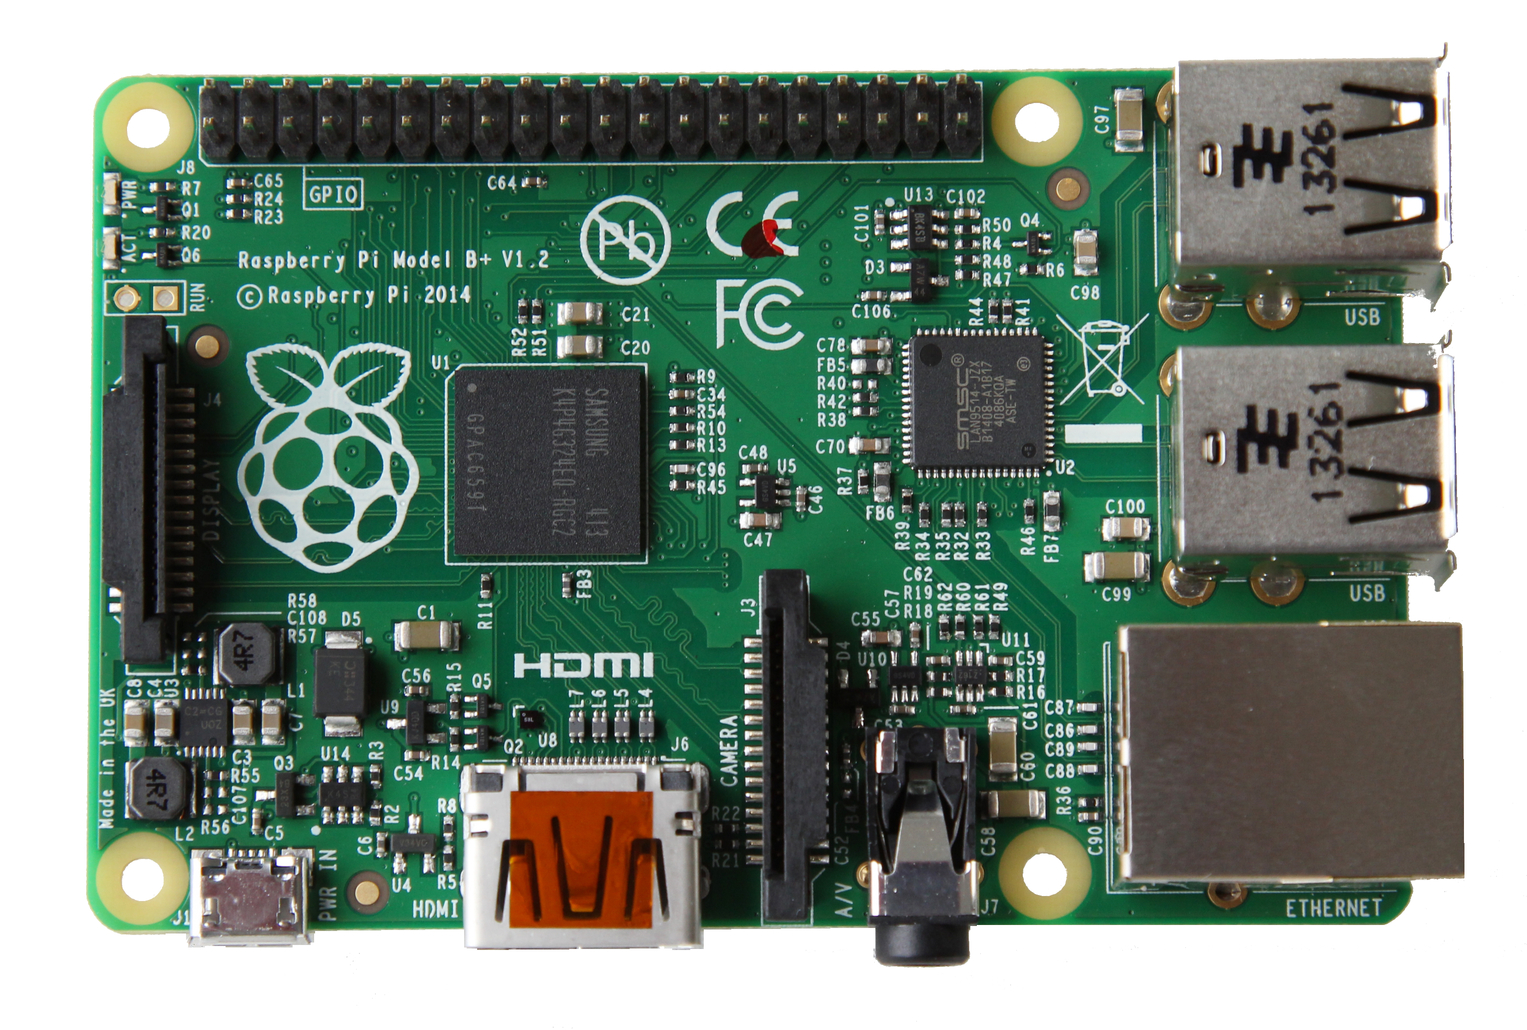
\includegraphics[width=\linewidth/2]{capitulo3/raspberry}
		\par\end{centering}
	\smallskip
	\caption{\label{fig:raspberry} Placa computadora Raspberry Pi.}
\end{figure} 

\smallskip

\subsection{Especificaciones técnicas}

La siguiente tabla ilustra las principales características del \textit{Raspberry Pi} \cite{raspberry}:

\smallskip

\begin{center}
	\begin{tabular}{|l|l|}
		\hline Modelo & Raspberry Pi B+ v1.2 \\
		\hline SoC & Broadcom BCM2835 \\
		\hline Procesador &  1176JZF-S @ 700 \textit{MHz} \\
		\hline Repertorio de instrucciones & ARMv6 (\textit{RISC} 32-\textit{bit}) \\
		\hline Memoria & 512 \textit{MB} @ 400 \textit{MHz} \\
		\hline Procesador gráfico & Broadcom VideoCore IV \\ 		
		\hline Almacenamiento & Micro-\acrshort{SD} 8 \textit{GB} \textit{class 10} \\
		\hline Salida de vídeo & \acrshort{HDMI} \\
		\hline Salida de audio & \textit{Jack} 3.5 \textit{mm}, \acrshort{HDMI} \\
		\hline Conectividad USB & 4 x \acrshort{USB} 2.0 \\
		\hline Conectividad de red & \textit{Ethernet} 100 \textit{Mbit/s} \\
		\hline Periféricos & 28xGPIO, \acrshort{UART}, \acrshort{I2C}, \acrshort{SPI} \\ 
		\hline Alimentación & 5V Micro-\acrshort{USB} o \acrshort{GPIO} \\
		\hline Consumo máximo & 1.8 \textit{A} (9 \textit{W}) \\ 
		\hline Sistema operativo & Raspbian (Linux 3.8) \\
		\hline 
	\end{tabular}
	\smallskip
	\captionof{table}{\label{tab:rapberry} Especificaciones del Raspberry Pi.}

\end{center}

\smallskip

\subsection{Pines de E/S}

Como hemos adelantado, la \acrshort{PCB} se conectará al \textit{Raspberry} a través de los conectores \acrshort{GPIO} (\textit{\acrlong{GPIO}}). Todos ellos se utilizarán de forma genérica, excepto el receptor del mando a distancia, que se comunica con la interfaz \textit{RS-232} y debe conectarse al \acrshort{UART} mediante el pin dedicado a tal periférico.

La asignación de pines es la que sigue:

\smallskip

\begin{figure}[H]
	\noindent \begin{centering}
		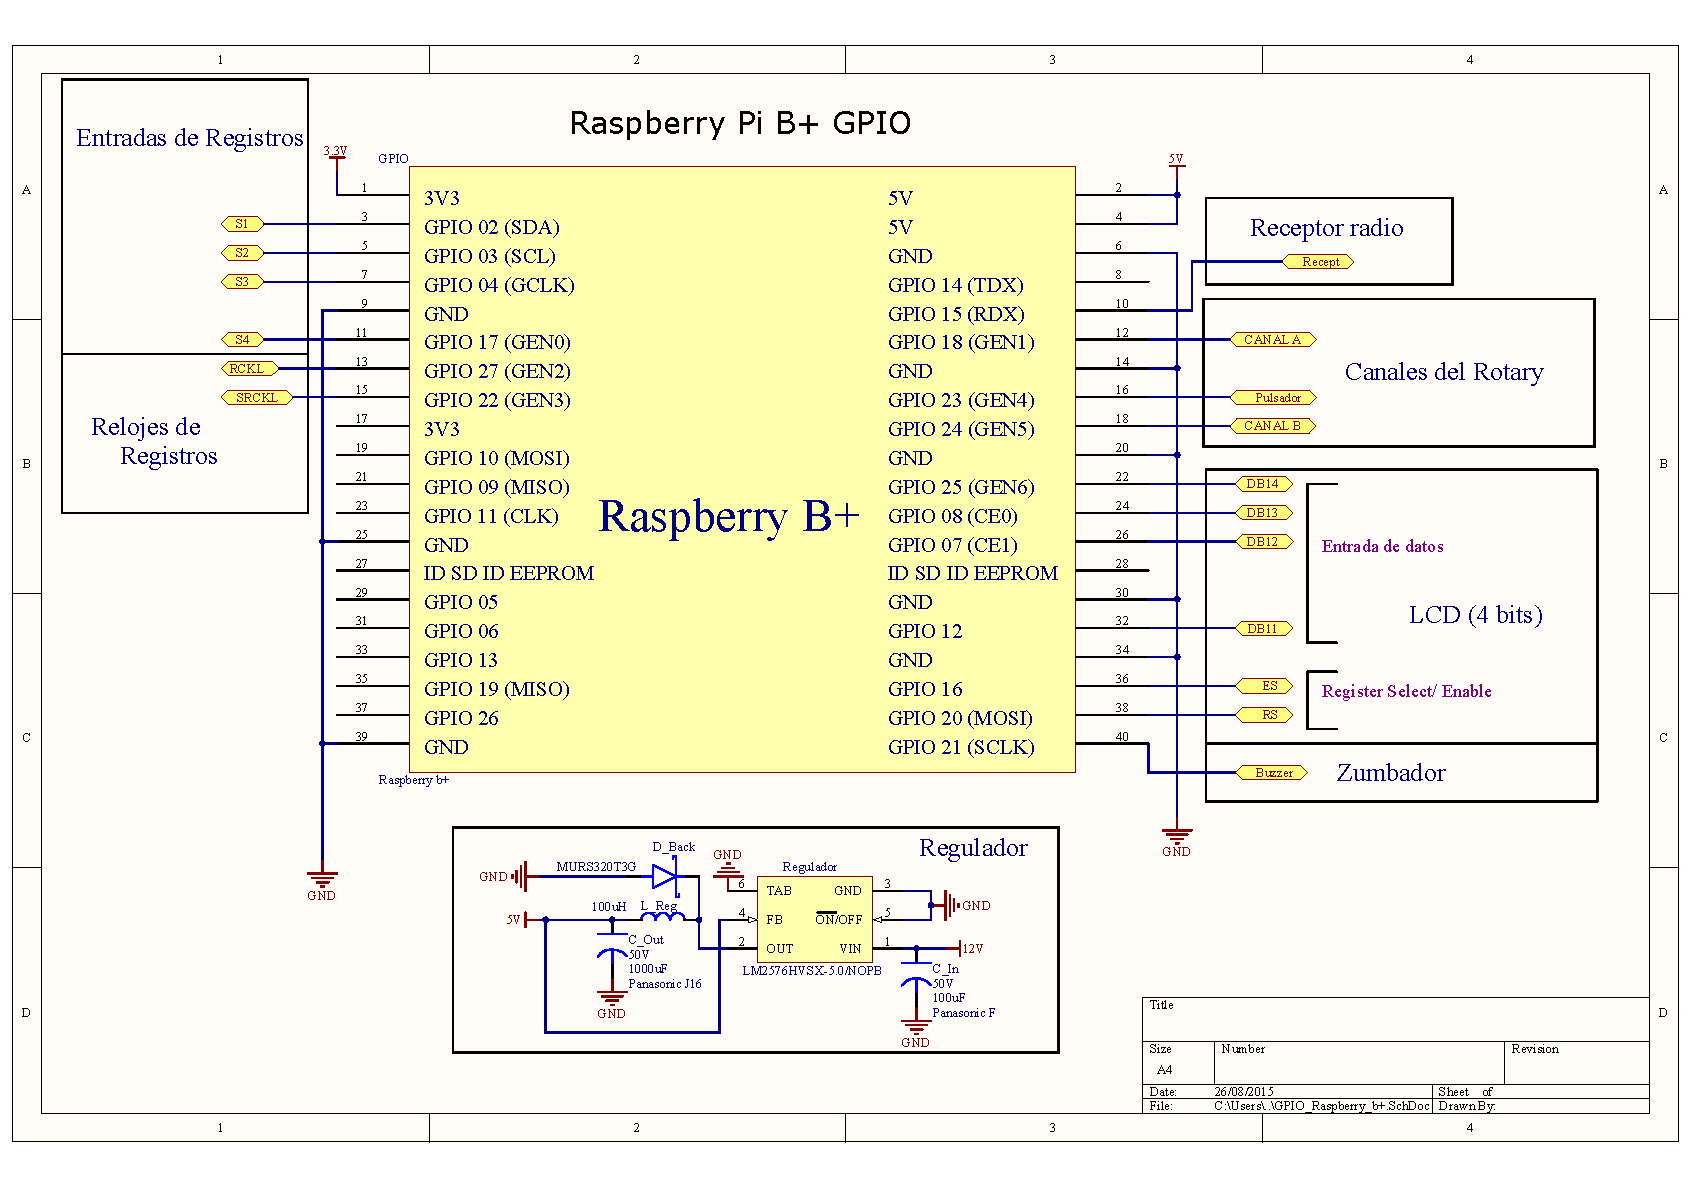
\includegraphics[width=\linewidth*2/3]{capitulo3/pcb_gpio}
		\par\end{centering}
	\smallskip
	\caption{\label{fig:pcb_gpio} Pines de conexión de la PCB con el Raspberry.}
\end{figure} 

\smallskip

\begin{center}
	\begin{tabular}{|l|l|}
		\hline \multicolumn{2}{|c|}{\textbf{Registros de desplazamiento}} \\
		\hline S1 (teclado barroco) & \acrshort{GPIO} 02 \\ 
		\hline S2 (teclado romántico) & \acrshort{GPIO} 03 \\ 
		\hline S3 (registros) & \acrshort{GPIO} 04 \\ 
		\hline S4 (\textit{pedalier}) & \acrshort{GPIO} 17 \\ 
		\hline RCLK (almacenamiento) & \acrshort{GPIO} 27 \\ 
		\hline SRCLK (desplazamiento) & \acrshort{GPIO} 22 \\ 
		\hline \multicolumn{2}{|c|}{\textbf{Receptor de radio}} \\
		\hline O/P-AF (datos) & \acrshort{GPIO} 15 (RDX) \\ 
		\hline \multicolumn{2}{|c|}{\textbf{Pantalla \acrshort{LCD}}} \\
		\hline DB4 (línea 4 del bus) & \acrshort{GPIO} 12 \\ 
		\hline DB5 (línea 5 del bus) & \acrshort{GPIO} 07 \\ 
		\hline DB6 (línea 6 del bus) & \acrshort{GPIO} 08 \\ 
		\hline DB7 (línea 7 del bus) & \acrshort{GPIO} 25 \\
		\hline RS (selección de registro) & \acrshort{GPIO} 20 \\ 
		\hline ES (habilitación de señal) & \acrshort{GPIO} 16 \\ 
		\hline \multicolumn{2}{|c|}{\textbf{Codificador rotatorio}} \\
		\hline Canal A (rotación) & \acrshort{GPIO} 18 \\ 
		\hline Canal B (rotación) & \acrshort{GPIO} 24 \\ 
		\hline Pulsación & \acrshort{GPIO} 23 \\ 
		\hline 
	\end{tabular}
	\smallskip
	\captionof{table}{\label{tab:gpio} Asignaciones de los pines del GPIO.}
\end{center}

\smallskip

\subsection{Sistema operativo}

A pesar de su reducido tamaño, \textit{Raspberry Pi} no es un microcontrolador, sino un microcomputador, con una cantidad notable de recursos \textit{hardware} y potencia de cálculo suficiente para albergar múltiples procesos funcionando concurrentemente. Esto hace necesario el uso de un sistema operativo.

Podemos encontrar varios sistemas operativos compatibles con este computador, pero nosotros vamos a utilizar el sistema oficial, \textit{Raspbian}, una distribución basada en \textit{Debian}, que incorpora el núcleo \textit{GNU/Linux} para la plataforma \textit{ARMv6}.

La introducción de un sistema operativo flexibiliza enormemente la gestión de los recursos \textit{hardware} de un ordenador y garantiza la convivencia equitativa de todos los procesos. Por contra, esto significa que ninguna aplicación podrá utilizar la \textit{CPU} a tiempo completo, ni se garantiza tiempo-real.

El \textit{BCM2835} posee un temporizador de 1 \textit{MHz}. Naturalmente, es inviable ofrecer una granularidad temporal tan fina al planificador; así, éste es llamado cada 10.000 \textit{ticks}, es decir, cada 10 \textit{ms}. Esto garantiza un uso adecuado de los recursos \textit{software} al tiempo que hace imposible realizar comunicaciones síncronas a alta velocidad mediante programación.

Además, la versión utilizada del núcleo Linux es apropiativa ---\textit{preemptive}---, lo que significa que una rutina en modo \textit{kernel} puede bloquearse para dar paso a un servicio de interrupción, incluso que una interrupción puede verse bloqueada por otra de mayor prioridad (interrupciones anidadas).

En conclusión, el uso de un sistema operativo de este tipo, a pesar de ser de gran utilidad, no garantiza sincronismo ni que una espera solicitada sea tan exacta como se pide.

\section{Formato de archivo MIDI}

El estándar \acrshort{MIDI} (\acrlong{MIDI}) es una interfaz que permite conectar instrumentos musicales electrónicos y computadoras. Comprende desde un protocolo electrónico hasta un formato de archivos, que se basa en una serie de eventos de control de parámetros musicales. \cite{wiki_midi}

Los datos de entrada a nuestro sistema consisten en archivos \acrshort{MIDI}, tal como se menciona en los requisitos. Este tipo de ficheros se presenta como un conjunto de bloques ---\textit{chunks}--- que contienen los eventos clasificados por pistas. Todos los valores numéricos están en formato \textit{big-endian}, detalle a tener en cuenta, ya que tanto la arquitectura x86 como ARM trabajan en \textit{little-endian}. \cite{midi}

\subsection{Bloque de cabecera}

El bloque de cabecera es siempre el primero, empieza por la firma "MThd" e incluye la siguiente información:

\smallskip

\begin{center}
	\begin{tabular}{|l|l|l|}
		\hline \multicolumn{1}{|c|}{\textbf{Longitud}} & \multicolumn{1}{c|}{\textbf{Descripción}} & \multicolumn{1}{c|}{\textbf{Valor}} \\
		\hline 4 bytes & Firma & "MThd" \\ 
		\hline 4 bytes & Tamaño & 6 \\ 
		\hline 2 bytes & Formato & 0--2 \\ 
		\hline 2 bytes & Número de pistas & 1--65535 \\ 
		\hline 2 bytes & División de tiempo &  \\ 
		\hline 
	\end{tabular}
	\smallskip
	\captionof{table}{\label{tab:midi_header} Contenido de la cabecera MIDI.}
\end{center}

\smallskip

\begin{description}
	\item[Formato] Es la forma en que se organizan las pistas. Puede ser:
	\begin{description}
		\item[0] Una sola pista.
		\item[1] Varias pistas, simultáneas.
		\item[2] Varias pistas, independientes.
	\end{description}
	
	\item[Número de pistas] Indica de cuántas pistas se compone el archivo. Obviamente, si el formato es 0, el valor de este campo será 1.
	
	\item[División de tiempo] Nos indica el significado de cada \textit{tick} de reloj del protocolo como divisiones de una negra (\quarternote). Valores típicos son 96, 120, 180, 192, 240, 360, 384, 480, 640, 720, 768 y 960 \textit{ticks}/\quarternote. Si el valor es negativo, el número indica en su lugar el número de \textit{ticks/fotograma}, habitualmente utilizado en realización de vídeo.
\end{description}

\subsection{Bloque de pista}

Una pista consta de una cabecera y de una lista de eventos, que termina con el meta-evento \textit{fin de pista}.

\smallskip

\begin{center}
	\begin{tabular}{|l|l|l|}
		\hline \multicolumn{1}{|c|}{\textbf{Longitud}} & \multicolumn{1}{c|}{\textbf{Descripción}} & \multicolumn{1}{c|}{\textbf{Valor}} \\
		\hline 4 bytes & Firma & "MTrk" \\ 
		\hline 4 bytes & Tamaño & 0-65535 \\  
		\hline 
	\end{tabular}
	\smallskip
	\captionof{table}{\label{tab:midi_track} Contenido de la cabecera de una pista MIDI.}
\end{center}

\smallskip

\subsection{Eventos MIDI}

Cada evento está formado por los siguientes campos:

\smallskip

\begin{center}
	\begin{tabular}{|l|l|}
		\hline \multicolumn{1}{|c|}{\textbf{Longitud}} & \multicolumn{1}{c|}{\textbf{Descripción}} \\
		\hline Variable & $\Delta$ \\ 
		\hline 1 byte & Tipo de evento y canal \\ 
		\hline 1 byte & Parámetro 1 \\ 
		\hline 1 byte & Parámetro 2 \\ 
		\hline 
	\end{tabular}
	\smallskip
	\captionof{table}{\label{tab:midi_evento} Especificación de un evento MIDI.}
\end{center}

\smallskip

\begin{description}
	\item[$\Delta$] Indica el número de \textit{ticks} que separan al evento actual del precedente.
	\item[Tipo de evento y canal] Los cuatro \textit{bits} más significativos corresponden al tipo de evento. Los otros cuatro marcan el canal \acrshort{MIDI}.
\end{description}

\smallskip

\begin{center}
	\begin{tabular}{|l|l|l|l|}
		\hline \multicolumn{4}{|c|}{\textbf{Tipos de evento}} \\
		\hline \multicolumn{1}{|c|}{\textbf{Valor}} & \multicolumn{1}{c|}{\textbf{Nombre}} & \multicolumn{1}{c|}{\textbf{Parámero 1}} & \multicolumn{1}{c|}{\textbf{Parámetro 2}} \\
		\hline 0x80 & NOTE-OFF & Nota & Velocidad \\
		\hline 0x90 & NOTE-ON & Nota & Velocidad \\
		\hline 0xA0 & NOTE-AFTERTOUCH & Nota & Velocidad \\
		\hline 0xB0 & CONTROLLER & Controlador & Valor \\
		\hline 0xC0 & PROGRAM-CHANGE & Programa &  \\
		\hline 0xD0 & CHANNEL-AFTERTOUCH & Velocidad &  \\
		\hline 0xE0 & PITCH-BEND & \multicolumn{2}{c|}{Valor} \\
		\hline 0xF0 & SYSTEM-EXCLUSIVE & \multicolumn{2}{c|}{} \\
		\hline 0xFF & Meta-evento & \multicolumn{2}{c|}{} \\
		\hline 
	\end{tabular}
	\smallskip
	\captionof{table}{\label{tab:midi_eventos} Eventos MIDI.}
\end{center}

\smallskip

\subsubsection{Meta-eventos}

Los metaeventos son mensajes de control que extienden la semántica de los eventos normales. Tienen la siguiente estructura:

\smallskip

\begin{center}
	\begin{tabular}{|l|l|}
		\hline \multicolumn{1}{|c|}{\textbf{Longitud}} & \multicolumn{1}{c|}{\textbf{Descripción}} \\
		\hline Variable & $\Delta$ \\ 
		\hline 1 byte & 0xFF \\
		\hline 1 byte & Tipo de metaevento \\
		\hline Variable & Longitud del argumento \\ 
		\hline (Longitud) & Valor del argumento \\ 
		\hline
	\end{tabular}
	\smallskip
	\captionof{table}{\label{tab:midi_mevaevento} Especificación de un meta-evento MIDI.}
\end{center}

\smallskip

Los tipos de meta-evento estándar son los siguientes:

\smallskip

\begin{center}
	\begin{tabular}{|l|l|}
		\hline \multicolumn{2}{|c|}{\textbf{Tipos de meta-evento}} \\
		\hline \multicolumn{1}{|c|}{\textbf{Valor}} & \multicolumn{1}{c|}{\textbf{Nombre}} \\
		\hline 0x00 & Número de secuencia \\
		\hline 0x01 & Texto \\
		\hline 0x02 & Noticia de \textit{copyright} \\
		\hline 0x03 & Nombre de la secuencia \\
		\hline 0x04 & Nombre del instrumento \\
		\hline 0x05 & Letra de la canción \\
		\hline 0x06 & Marca \\
		\hline 0x07 & Punto de corte \\
		\hline 0x08 & Nombre del programa \\
		\hline 0x09 & Nombre del dispositivo \\
		\hline 0x20 & Prefijo del canal \\
		\hline 0x2F & Fin de pista \\
		\hline 0x51 & \textit{Tempo} ($\mu s/\quarternote$) \\
		\hline 0x54 & Desplazamiento temporal \\
		\hline 0x58 & Indicación de compás \\
		\hline 0x59 & Indicación de tonalidad \\
		\hline 0x7F & Reservado para el secuenciador \\
		\hline 
	\end{tabular}
	\smallskip
	\captionof{table}{\label{tab:midi_metaeventos} Meta-eventos MIDI.}
\end{center}

\smallskip

\subsubsection{Notas}

Las notas en \acrshort{MIDI} se indican numéricamente, en base 0, asignando valores a las notas cromáticas a partir de \textit{Do -1}. Por ejemplo, al \textit{Do central (Do 4)} le corresponde el valor 60.

\section{Esquema de interconexión general}

Todos los elementos que hemos descrito conformarán la parte \textit{hardware} del sistema y establecerán una conexión cuyos extremos son el computador \textit{Raspberry Pi} y los mecanismos que interactuarán con la consola del órgano.

A continuación presentamos un diagrama que describe a \textit{grosso modo} la conexión lógica entre todos los elementos \textit{hardware}:

\smallskip

\begin{figure}[H]
	\noindent \begin{centering}
		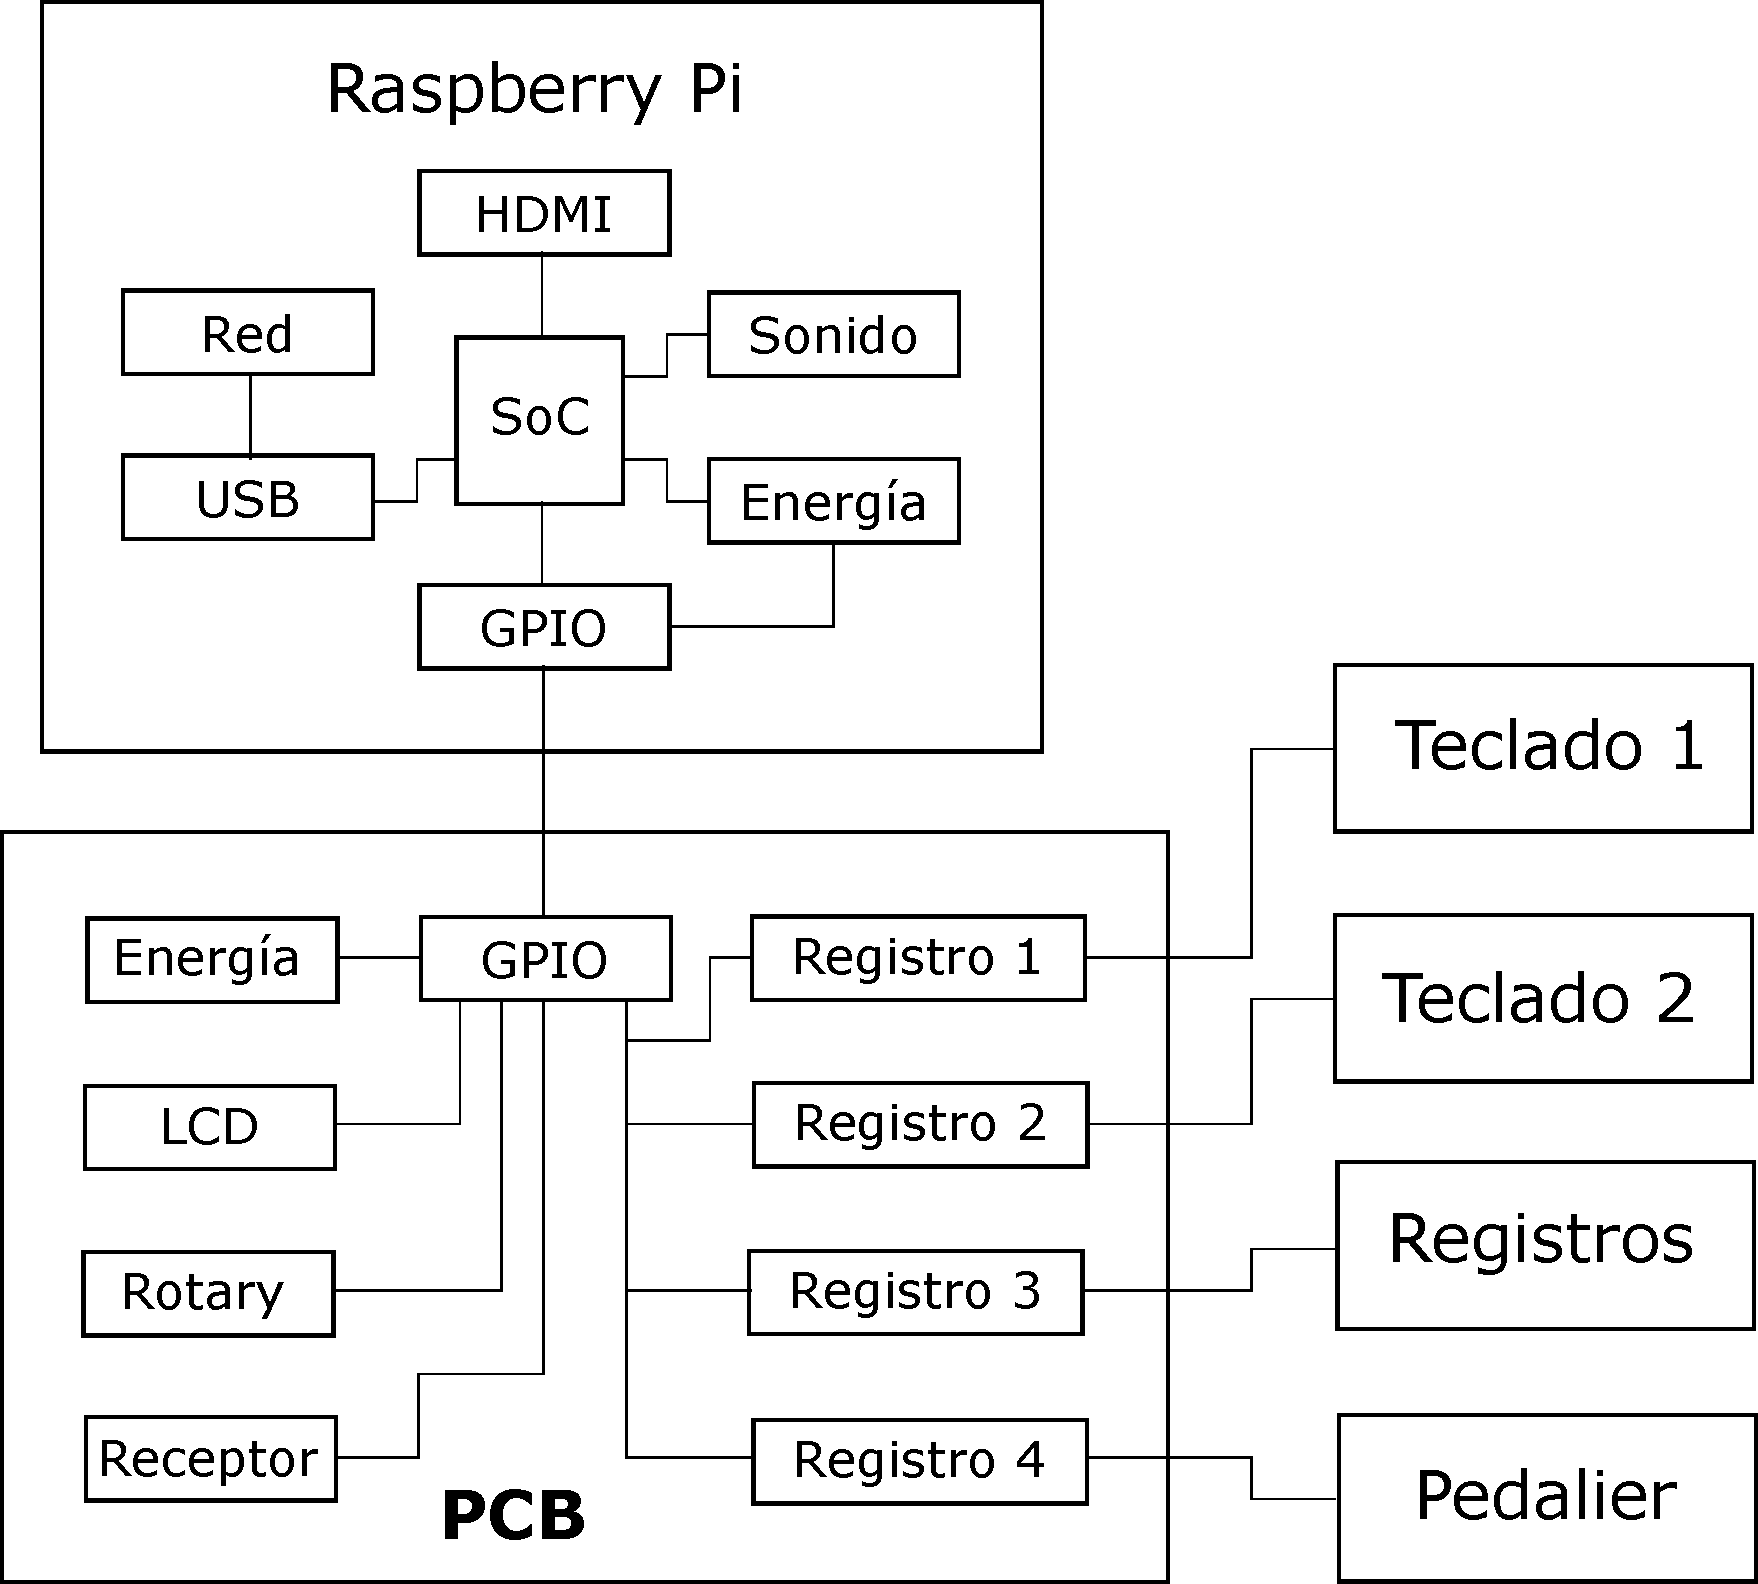
\includegraphics[width=\linewidth*2/3]{capitulo3/hardware}
		\par\end{centering}
	\smallskip
	\caption{\label{fig:hardware} Conexión lógica entre los elementos hardware.}
\end{figure} 

\smallskip

La \acrshort{PCB} incorpora una fuente de alimentación para el \textit{Raspberry}, que está conectada mediante la interfaz \acrshort{GPIO}. Todas las conexiones harán funcionar los mecanismos del órgano, pasando por los registros de desplazamiento, que retendrán el estado.

El resto de periféricos nos serán de utilidad para desarrollar un sistema que cumplirá todos los requisitos contemplados en el capítulo \ref{cap:capitulo_2}.

\clearpage{\cleardoublepage}
\clearpage{\pagestyle{empty}\cleardoublepage}
%
\chapter{Diseño del sistema.}
\label{cap: capitulo_4}

En este capítulo vamos a detallar cómo hemos concebido la solución a los requisitos \textit{software}, teniendo en cuenta los correspondientes al \textit{hardware} y a partir de los elementos que hemos detallado en el capítulo anterior.

\section{Planteamiento}

Como idea más abstracta, el \textit{software} que tenemos que diseñar consiste en un reproductor de archivos \textit{MIDI}, que recibe el fichero y lo envía a la \textit{PCB} a través del \textit{GPIO}. Por supuesto, la reproducción estará controlada por el usuario:

\smallskip

\begin{figure}[H]
	\noindent \begin{centering}
		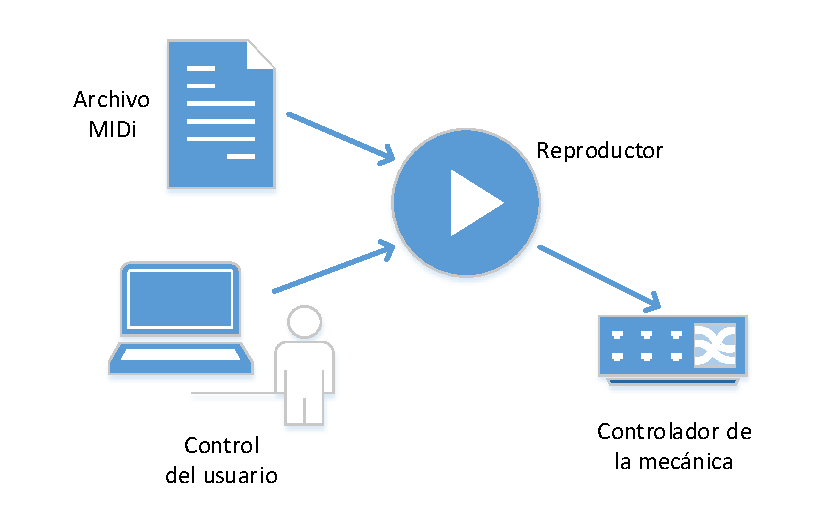
\includegraphics[width=\linewidth/2]{capitulo4/idea}
		\par\end{centering}
	\smallskip
	\caption{\label{fig:idea} Planteamiento inicial.}
\end{figure} 

\smallskip

Luego, dividiremos el sistema en cuatro grandes bloques. Respecto al de control, se requiere varias formas de acceder al sistema:

\begin{enumerate}
	\item Un \textit{software} controlador principal, que cubra todos los casos de uso, y sea fácil de instalar y utilizar, con preferencia de que sea multiplataforma.
	
	\item Un mando a distancia, que altere la reproducción.
	
	\item Un control reducido empotrado en la \textit{PCB}.
\end{enumerate}

Atendiendo a los requisitos del primer controlador y a las prestaciones del \textit{Raspberry Pi}, y con objeto de eliminar la necesidad de instalar y mantener aplicaciones en otro sistema, decidimos enfocar la solución como una interfaz \textit{web} con un servidor alojado en el \textit{Raspberry Pi}. De esta forma podemos llegar fácilmente a cualquier sistema operativo de escritorio, incluso es fácilmente adaptable a dispositivos móviles.

Sin embargo, el reproductor no puede funcionar dentro de un servidor \textit{web}, ya que éstos atienden peticiones sin estado, y se cierran automáticamente después de devolver la información. Por ello, vamos a diseñar el reproductor como un \textit{demonio} de \textit{Linux}, junto con sus módulos auxiliares.

En último lugar, necesitamos almacenar información de los archivos \textit{MIDI}, listas de reproducción y asignaciones del mando en memoria persistente. Una base de datos nos permitiría guardar toda esa información de manera estructurada y coherente, además de ser fácilmente accesible por todos los componentes del sistema.

\section{Demonio del reproductor}

Un demonio ---\textit{daemon}--- es un proceso que se ejecuta en segundo plano en la fase de arranque del sistema operativo, y no interactúa directamente con el usuario, sino que se comunica con otros procesos a través de herramientas proporcionadas por el sistema operativo.

Este programa será el núcleo de nuestro sistema, y ofrecerá las siguientes vías para comunicarse:

\begin{enumerate}
	\item Un \textit{socket} local de \textit{Linux}. Será usado principalmente por la interfaz \textit{web}, pero es una forma flexible y eficiente para que lo hagan más aplicaciones.
	
	\item El puerto en serie (\textit{UART}) del \textit{Raspberry Pi}, para recibir órdenes del mando.
	
	\item Los pines del \textit{GPIO} correspondientes al codificador rotatorio y el \textit{LCD}, para la interfaz reducida.
\end{enumerate}

Así, el esquema de uso de los distintos componentes queda así:

\smallskip

\begin{figure}[H]
	\noindent \begin{centering}
		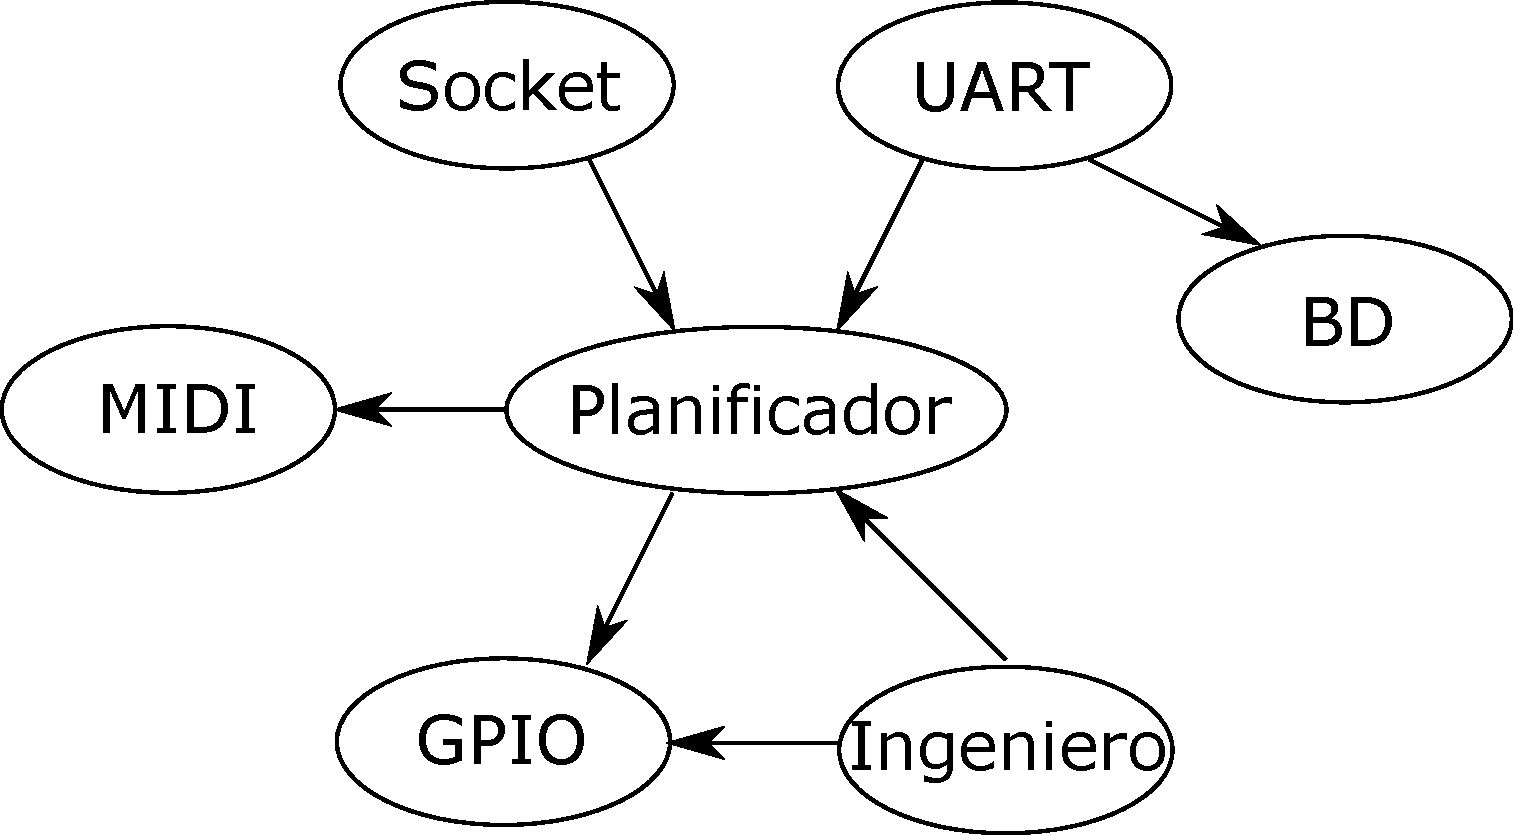
\includegraphics[width=\linewidth/2]{capitulo4/daemon}
		\par\end{centering}
	\smallskip
	\caption{\label{fig:daemon} Diagrama de uso entre los componentes del reproductor.}
\end{figure} 

\smallskip

\subsection{Descodificador de MIDI}

Como hemos detallado más arriba, el formato \textit{MIDI} expone los eventos de control en orden temporal, clasificados por pistas, habitualmente simultáneas. Debemos proporcionar una estructura de datos que permita mantener cada archivo a reproducir en memoria y facilitar el acceso individual a cada pista.

Concebimos la estructura de datos como un conjunto de listas enlazadas de eventos. El tamaño de los eventos normales es constante, sin embargo, los meta-eventos extienden la semántica con una cadena de datos.

\subsubsection{Estructura \textit{midifile\_t}}

Define un archivo \textit{MIDI}. Sus campos son:

\begin{description}
	\item[format : \textit{enum}] Formato del archivo. Puede tener los siguientes valores enumerados:
	
	\begin{description}
		\item[SINGLE\_TRACK] Una sola pista.
		\item[MULTIPLE\_SIMULTANEOUS] Varias pistas, simultáneas.
		\item[MULTIPLE\_INDEPENDENT] Varias pistas, independientes.
	\end{description}
	
	\item[ntracks : \textit{word}] Número de pistas.
	
	\item[division : \textit{enum}] Unidad de medida de la división de tiempo:
	
	\begin{description}
		\item[TICKS\ PER\ BEAT] La división se especifica en \textit{ticks}/\quarternote.
		\item[FRAMES\_PER\_SECOND] La división se especifica en \textit{ticks/fotograma}.
	\end{description}
	
	\item[tracks : \textit{array(midievent\_t)}] Conjunto de listas de eventos; cada lista corresponde a una pista.

\end{description}

\subsubsection{Estructura midievent\_t}

Define un evento MIDI.

\begin{description}
	\item[delta : \textit{dword}] Separación temporal respecto al evento anterior.
	\item[type : \textit{enum}] Tipo de evento. Se enumeran en el capítulo anterior.
	\item[param1 : \textit{byte}] Valor del primer parámetro, dependiendo del tipo de evento.
	\item[param2 : \textit{byte}] Valor del segundo parámetro, dependiendo del tipo de evento.
	\item[metaevent : \textit{metaevent\_t}] Información del metaevento, si procede.
	\item[next : \textit{midievent\_t}] Evento siguiente, si procede.
\end{description}

\subsubsection{Estructura \textit{metaevent\_t}}

Define un meta-evento.

\begin{description}
	\item[type : \textit{emum}] Tipo de metaevento. Se enumeran en el capítulo anterior.
	\item[length : \textit{dword}] Longitud de la cadena de datos, en \textit{bytes}.
	\item[data : \textit{string}] Cadena de datos correspondientes al meta-evento.
\end{description}

\subsubsection{Funciones}

\begin{description}[style=nextline]
	\item[midifile\_init (score, path) : \textit{int}] 
	Lee un archivo MIDI e inicializa la estructura recibida. 
	
	\begin{description}
		\item[score : \textit{midifile\_t}] Archivo \textit{MIDI} sin inicializar.
		\item[path : \textit{string}] Ruta del fichero a leer.
	\end{description}
	
	Devuelve 0 en caso de éxito, o -1 en caso de error.
	
	\item[midifile\_destroy (file)] 
	Elimina una estructura y libera su memoria.
	
	\begin{description}
		\item[file : \textit{midifile\_t}] Archivo \textit{MIDI}.
	\end{description}
	
	\item[midifile\_duration (file) : \textit{dword}] 
	Obtener la duración de una pieza.
	
	\begin{description}
		\item[file : \textit{midifile\_t}] Archivo \textit{MIDI}.
	\end{description}
	
	Devuelve la duración de la pieza, en \textit{segundos}.
	
	\item[metaevent\_tempo (event) : \textit{dword}] 
	Obtener el \textit{tempo} de la pieza.
	
	\begin{description}
		\item[event : \textit{metaevent\_t}] Meta-vento.
	\end{description}
	
	Devuelve el \textit{tempo} de la pieza en \textit{$\mu s$/\quarternote}.
	
\end{description}

\subsubsection{Diagrama de uso}

El módulo \textit{MIDI} solo se usa directamente a través del planificador. Éste se encarga de gestionar las partituras, y ordenar su eliminación cuando sea necesario.

\smallskip

\begin{figure}[H]
	\noindent \begin{centering}
		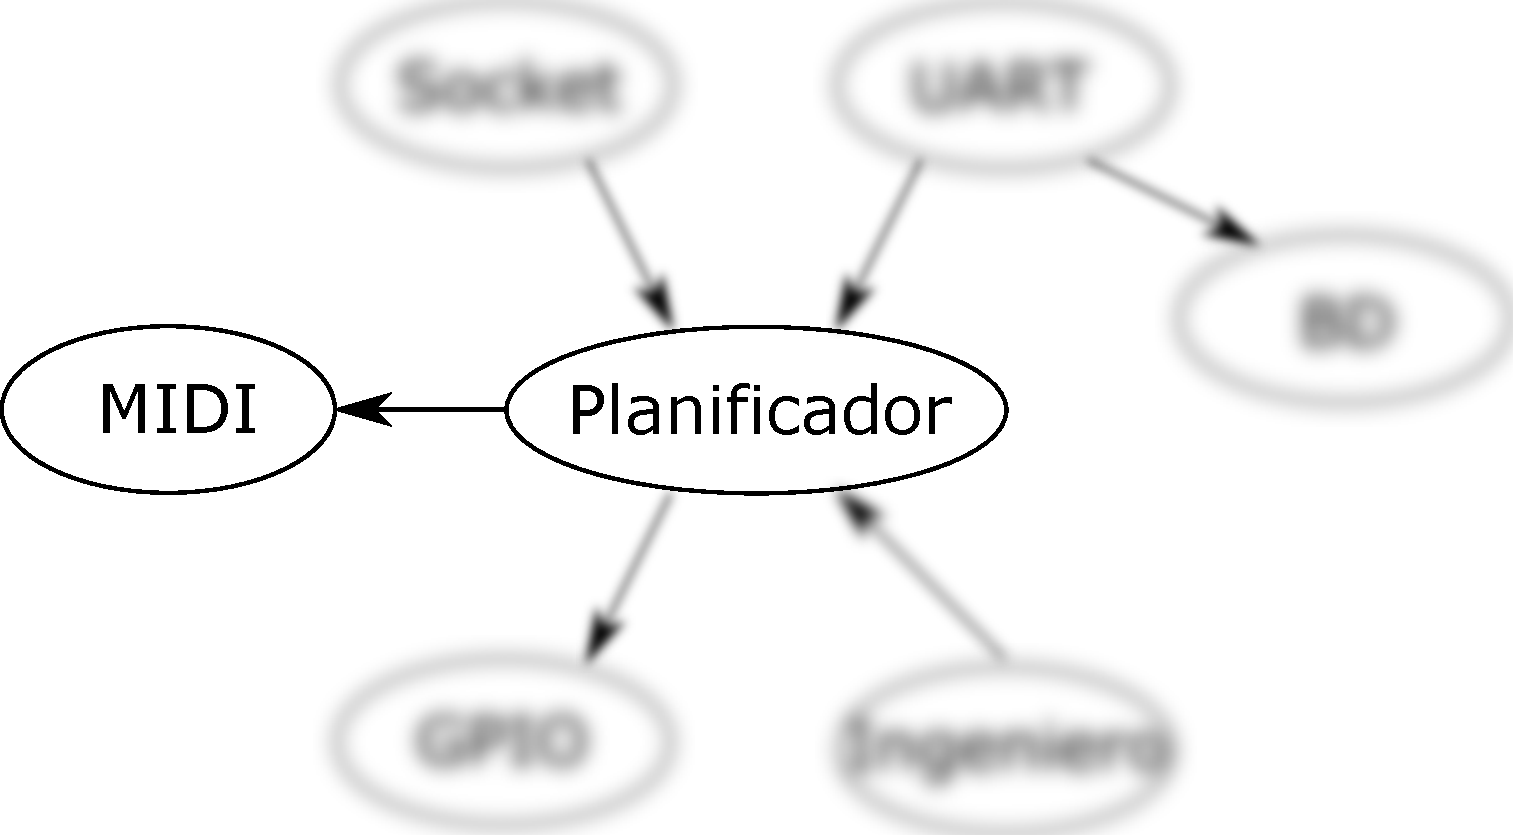
\includegraphics[width=\linewidth/2]{capitulo4/daemon_midi}
		\par\end{centering}
	\smallskip
	\caption{\label{fig:daemon_midi} Diagrama de uso del módulo MIDI.}
\end{figure} 

\smallskip

\subsection{Control por socket}

Un \textit{socket} un mecanismo de comunicación inter-proceso ---\textit{IPC (inter-process communication)} que proporciona \textit{Linux} y enviar y recibir datagramas en modo \textit{duplex}, bien dentro de la misma máquina (\textit{socket} local) o en una red (\textit{socket} de Internet).

Vamos a crear un \textit{socket} local, accesible desde el sistema de archivos de \textit{Linux}, que escuche peticiones de los clientes que se conecten, utilizando una interfaz basada en lenguaje natural, que explicaremos a continuación.

Las funciones diseñadas son las siguientes:

\begin{description}[style=nextline]
	\item[socket\_init (uid, gid) : \textit{dword}]
	Inicializar el \textit{socket} con el ID de usuario y grupo indicados.
	
	\begin{description}
		\item[uid : \textit{dword}] ID de usuario en Linux.
		\item[gid : \textit{dword}] ID de grupo en Linux.
	\end{description}
	
	Devuelve 0 en caso de éxito y -1 en caso de error.
	
	\item[socket\_destroy ()]
	Cierra el \textit{socket}.
	
	\item[socket\_loop ()]
	Despliega una hebra con un bucle de escucha y atiende las peticiones.
	
\end{description}

\subsubsection{Diagrama de uso}

El módulo correspondiente al \textit{socket} solamente interacciona internamente con el planificador, al que transmite adecuadamente las órdenes recibidas.

\smallskip

\begin{figure}[H]
	\noindent \begin{centering}
		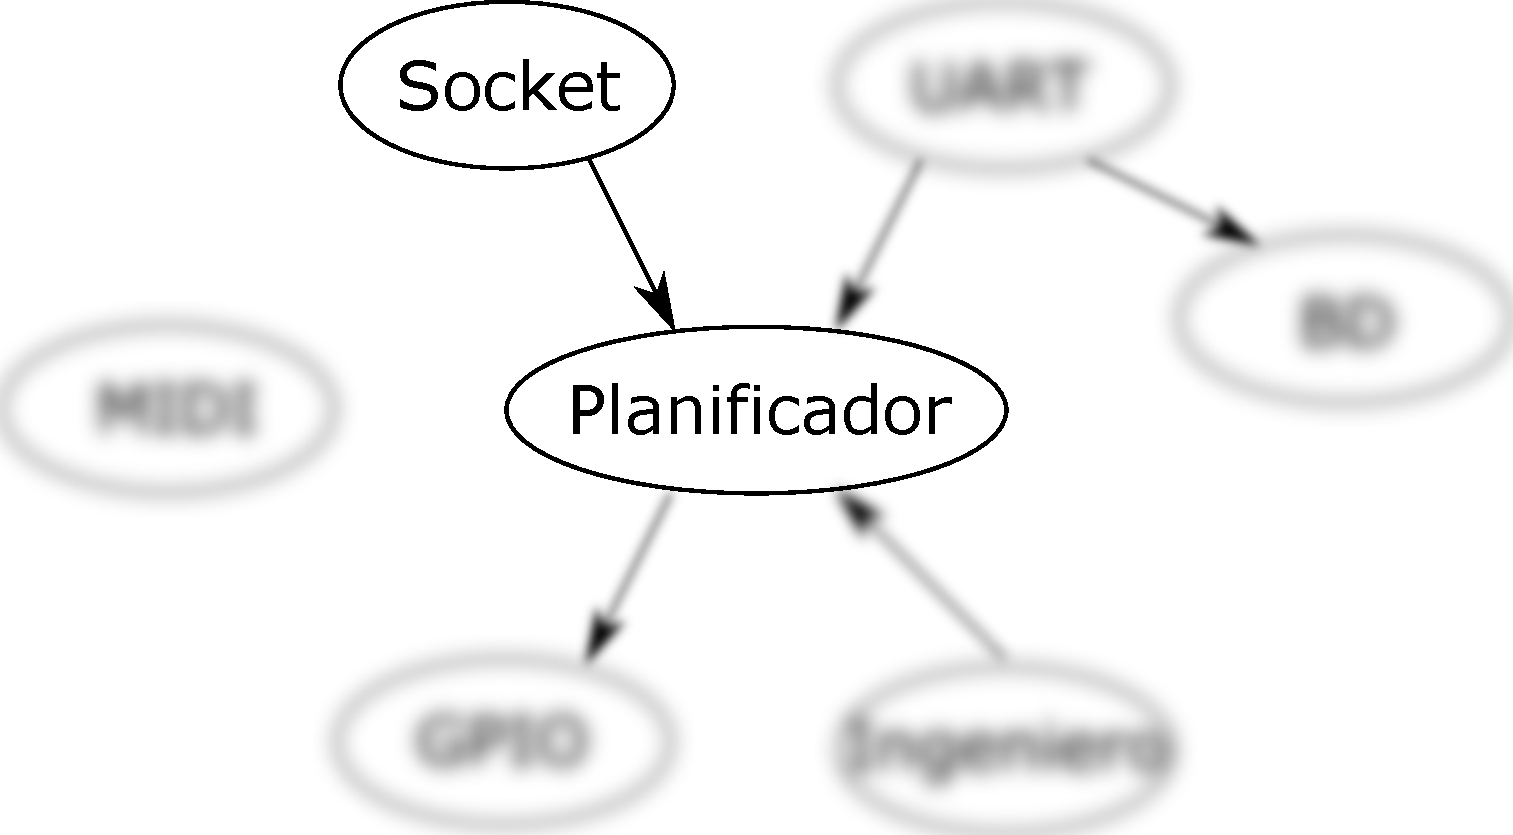
\includegraphics[width=\linewidth/2]{capitulo4/daemon_socket}
		\par\end{centering}
	\smallskip
	\caption{\label{fig:daemon_socket} Diagrama de uso del servidor \textit{socket}.}
\end{figure} 

\smallskip

\subsubsection{Lenguaje de la interfaz}

El \textit{socket} reconocerá y ejecutará una serie de órdenes, emitiendo siempre una respuesta:

\begin{description}
	\item[PLAY <archivo> [ <archivo>*]] Reproducir una lista de archivos MIDI, indicando las rutas completa, separadas por espacios. Respuesta:
	
	\begin{description}
		\item[OK] en caso de éxito.
		\item[ERROR] en caso de error o estar en modo Ingeniería.
	\end{description}
	
	\item[PLAYLOOP <archivo> [ <archivo>*]] Reproducir en bucle una lista de archivos MIDI, indicando las rutas completa, separadas por espacios. Respuesta:
	
	\begin{description}
		\item[OK] en caso de éxito.
		\item[ERROR] en caso de error o estar en modo Ingeniería.
	\end{description}
	
	\item[PAUSE] Pausar la reproducción. Silencia las notas pero manteniendo el estado. Respuesta:
	
	\begin{description}
		\item[OK] en caso de éxito.
		\item[ERROR] en caso de error, como estar detenido, o en modo Ingeniería.
	\end{description}
	
	\item[RESUME] Reanuda la reproducción en el punto en que se pausó. Respuesta:
	
	\begin{description}
		\item[OK] en caso de éxito.
		\item[ERROR] en caso de error, como no estar pausado, o en modo Ingeniería.
	\end{description}
	
	\item[STOP] Detiene completamente la reproducción y libera la lista de reproducción. Respuesta:
	
	\begin{description}
		\item[OK] en caso de éxito.
		\item[ERROR] en caso de error o estar en modo Ingeniería.
	\end{description}
	
	\item[STATUS] Consulta el estado del reproductor. Respuesta:
	
	\begin{description}
		\item[PLAYING <archivo>] Reproduciendo el archivo cuya ruta absoluta se especifica.
		\item[PAUSED <archivo>] Pausado en un punto del archivo cuya ruta se indica.
		\item[STOPPED] Detenido. Es el estado inicial.
		\item[ENGINEER] En modo Ingeniería. No se puede reproducir nada hasta desbloquearse.
	\end{description}
	
\end{description}

\subsection{Control del mando}

Como hemos indicado en el capítulo anterior, el receptor del mando a distancia está conectado al \textit{Raspberry Pi} a través de los pines correspondientes al dispositivo \textit{UART} ---\textit{Universal Asynchronus Receiver-Transmiter}---, que controla los puertos serie.

Este módulo tiene una topología análoga al control por \textit{socket}, tan solo cambia el origen y la forma de entrada de los datos. Establecerá una comunicación con el puerto serie e iniciará un bucle de escucha. La sintaxis del mensaje, como ya sabemos, es:

\begin{center}
	<Nº serie (7 \textit{bytes})> <Botón (1 \textit{byte})> <CRLF>
\end{center}

De esta forma, el servicio tan solo debe verificar el nº de serie y ejecutar la orden correspondiente.

Además de reconocer la pulsación del mando, es necesario consultar en la base de datos, que detallaremos más adelante, la lista que corresponde al botón pulsado y los archivos contenidos, que serán transmitidos al planificador.

Las funciones correspondientes a este módulo son las siguientes:

\begin{description}[style=nextline]
	\item[uart\_init () : \textit{dword}]
	Establece comunicación con el puerto serie.
	
	Devuelve 0 en caso de éxito y -1 en caso de error.
	
	\item[uart\_destroy ()]
	Cierra la comunicación.
	
	\item[uart\_loop ()]
	Despliega una hebra con un bucle de escucha y ejecuta las órdenes.
	
\end{description}

\subsubsection{Diagrama de uso}

Este bloque interacciona con el planificador en unos términos similares al \textit{socket}, y utiliza la interfaz de la base de datos.

\smallskip

\begin{figure}[H]
	\noindent \begin{centering}
		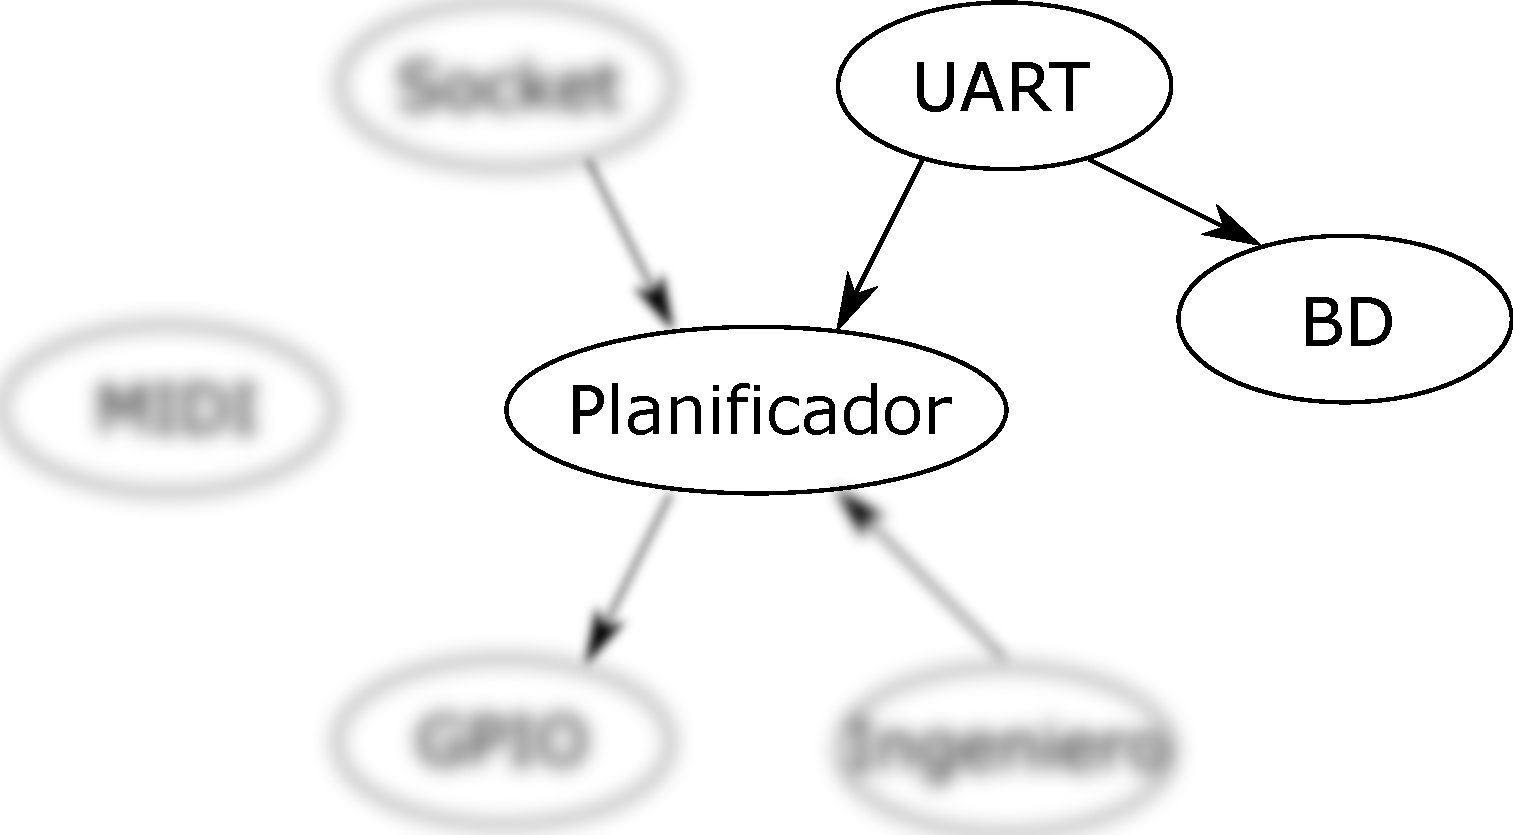
\includegraphics[width=\linewidth/2]{capitulo4/daemon_uart}
		\par\end{centering}
	\smallskip
	\caption{\label{fig:daemon_uart} Diagrama de uso del receptor de radio.}
\end{figure} 

\smallskip

\subsection{Comunicación con la base de datos}

La información relativa a la lista de reproducción asignada a un botón, así como la lista de partituras correspondientes, residirán en una base de datos, que definiremos próximamente. Así, enmarcaremos un nuevo módulo dedicado a consultar la información requerida, ofreciendo una interfaz independiente del sistema de gestión de bases de datos que utilicemos, y de la propia base de datos, mediante las siguientes funciones:

\begin{description}[style=nextline]
	\item[db\_init () : \textit{dword}]
	Inicia la comunicación con el gestor de bases de datos. Devuelve 0 en caso de éxito y -1 en caso de error.
	
	\item[db\_destroy ()]
	Cierra la comunicación.
	
	\item[db\_query (scores, idshortcut) : \textit{dword}]
	Realiza la consulta mencionada, asignando a \textit{scores} la lista de piezas a reproducir.
	
	\begin{description}
		\item[scores : \textit{array(string)}] Lista de rutas a las piezas.
		\item[idshortcut : \textit{dword}] ID del botón que se ha pulsado en el mando.
	\end{description}
	
	Devuelve el número de piezas asignadas (pudiendo ser 0), o -1 en caso de error.
	
\end{description}

\subsubsection{Diagrama de uso}

La interfaz de la base de datos es utilizada exclusivamente por el servidor del receptor de radio, sin perjuicio de que en un futuro podamos extender su funcionalidad, por lo que la hemos separado lógicamente del módulo \textit{UART}. El diagrama de uso es el siguiente:

\smallskip

\begin{figure}[H]
	\noindent \begin{centering}
		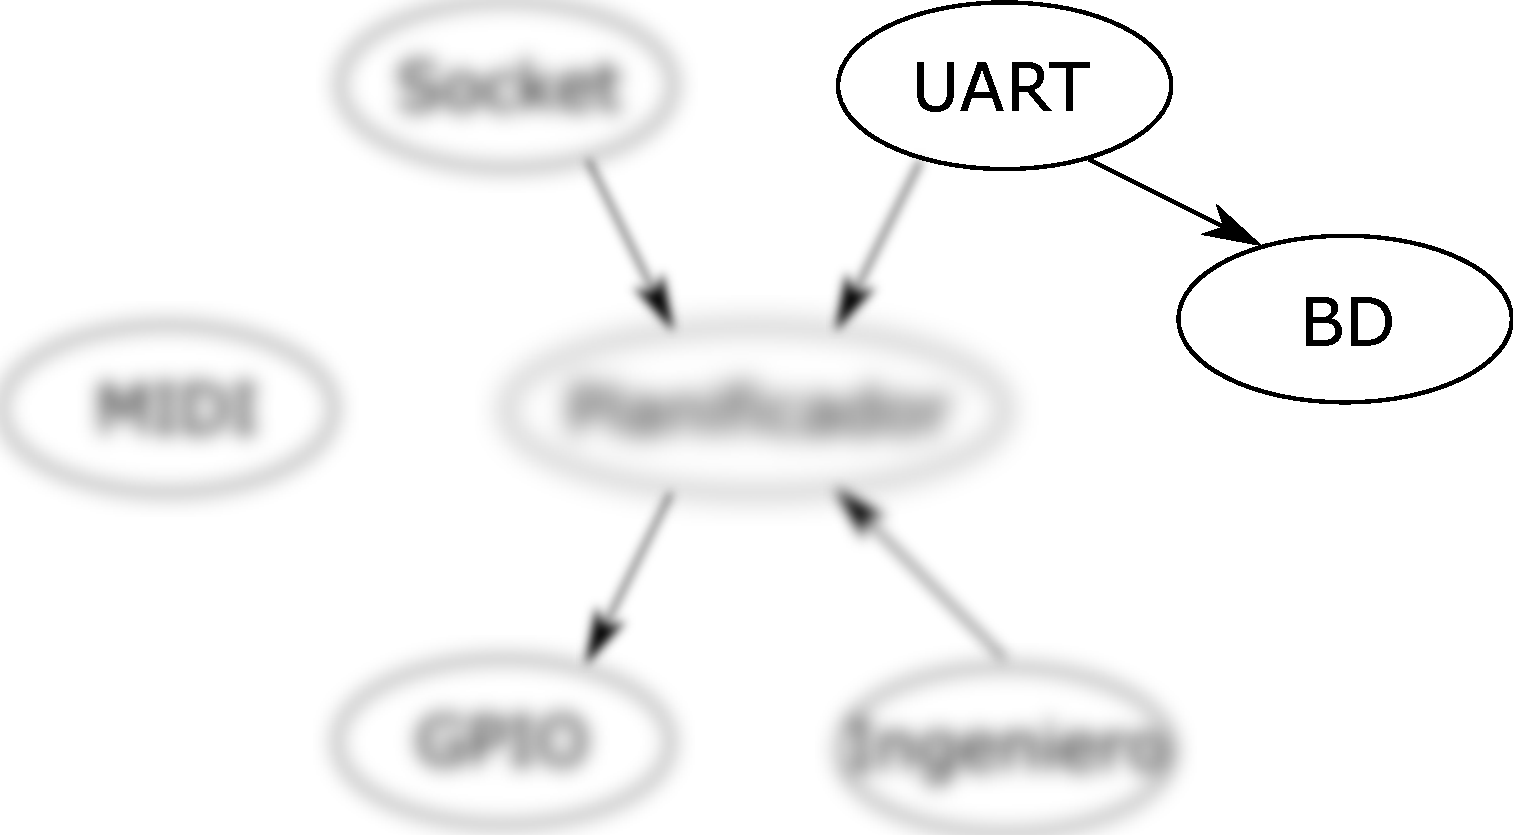
\includegraphics[width=\linewidth/2]{capitulo4/daemon_bd}
		\par\end{centering}
	\smallskip
	\caption{\label{fig:daemon_bd} Diagrama de uso de la interfaz de base de datos.}
\end{figure} 

\smallskip

\subsection{Planificador}

El planificador es la pieza principal del reproductor. Recibe las órdenes de los controladores y la lista de partituras a ejecutar. Una a una las lee con ayuda del módulo \textit{MIDI} y planifica los eventos de todas las pistas para lanzarlos a la salida en el momento necesario.

Al igual que otros módulos, utiliza una hebra para reproducir los archivos, pero en este caso es una hebra dinámica, que podrá ser iniciada, pausada y detenida por el resto de procesos, por lo que hay que tener en cuenta los problemas de concurrencia para garantizar la consistencia del sistema.

La interfaz que el planificador ofrece es la que sigue:

\begin{description}[style=nextline]
	\item[player\_start (playlist, n, loop) : \textit{dword}]
	Inicia la reproducción de una lista de archivos. Si ya estaba reproduciendo una lista, primero detiene la reproducción y elimina la lista antigua.
	
	\begin{description}
		\item[playlist : \textit{array(string)}] Lista de rutas absolutas a los archivos que queremos reproducir.
		\item[n : \textit{dword}] Número de piezas que se han transmitido en el parámetro anterior.
		\item[loop : \textit{bool}] Utilizar (1) o no (0) reproducción en bucle.
	\end{description}
	
	Devuelve 0 en caso de éxito o -1 en caso de error.
	
	\item[player\_pause () : \textit{dword}]
	Pausa la reproducción, si estaba activa. Devuelve 0 en caso de éxito o -1 en caso de error.
	
	\item[player\_stop () : \textit{dword}]
	Detiene completamente la reproducción, si estaba activa o pausada. Si estaba parado, no hace nada. Devuelve 0 en caso de éxito o -1 en caso de error.
	
	\item[player\_wait () : \textit{dword}]
	Espera a que el reproductor se detenga. Solo tiene sentido llamarla en caso de no estar reproduciendo en bucle. Devuelve 0 en caso de éxito o -1 en caso de error.
	
	\item[player\_state (file) : \textit{enum}]
	Indica el estado actual del planificador. Tales estados se detallan en el apartado siguiente.
	
	\begin{description}
		\item[file : \textit{string}] Es un parámetro de salida, sobre él se escribe el nombre del archivo que se estaba reproduciendo. Solo es válido si el reproductor está activo o en pausa.
	\end{description}
	
	Devuelve el estado actual del reproductor, a saber entre los estados contemplados en la máquina.
	
	\item[player\_engineer\_enter () : \textit{dword}]
	Detiene el reproductor, bloquea el planificador y entra en modo Ingeniería. Devuelve 0 en caso de éxito o -1 en caso de error, como estar ya dentro del modo Ingeniería.
	
	\item[player\_engineer\_exit () : \textit{dword}]
	Sale del modo Ingeniería y debloquea el planificador. Devuelve 0 en caso de éxito o -1 en caso de error, como no estar dentro del modo Ingeniería.
	
\end{description}

\subsubsection{Máquina de estados}

Para gestionar su funcionamiento, el planificador utiliza una pequeña cantidad de estados, que mostramos a continuación:

\smallskip

\begin{figure}[H]
	\noindent \begin{centering}
		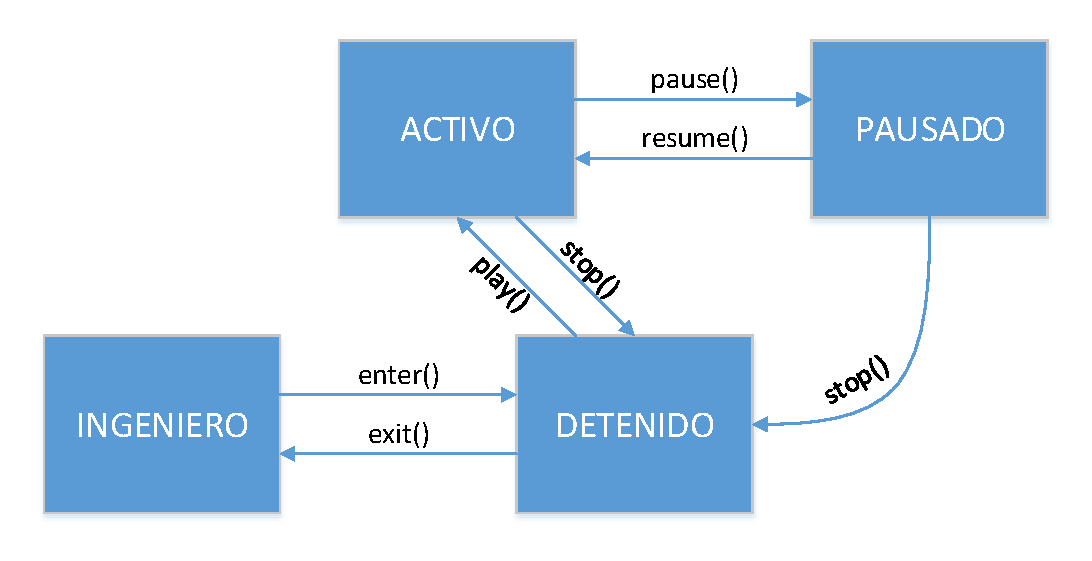
\includegraphics[width=\linewidth/2]{capitulo4/sched}
		\par\end{centering}
	\smallskip
	\caption{\label{fig:sched} Diagrama de estados del planificador.}
\end{figure} 

\smallskip

\begin{description}
	\item[Activo] En funcionamiento, reproduciendo activamente una partitura.
	\item[Pausado] No reproduce, mantiene el estado del órgano en el módulo de salida.
	\item[Parado] En espera. Es el estado inicial.
	\item[Ingeniero] Bloqueado, en modo Ingeniería. Ha cedido el control del módulo de salida.
\end{description}

\subsubsection{Algoritmo básico}

Para que todas las pistas se ejecuten simultáneamente, el planificador recorre en cada ciclo todas las listas, avanzando mientras sea el momento de ejecutar el evento correspondiente ($\Delta=0$). Cuando se ha llegado a un evento con $\Delta > 0$ en todas las pistas, se busca el menor valor y se resta a todos los \textit{deltas}. A continuación, se solicita al sistema operativo la espera correspondiente al tiempo restado, y se repite el ciclo. El algoritmo termina cuando todas las pistas han llegado al final.

\begin{algorithmic}
	\LOOP
		\STATE $mindelta \gets \infty$
		\STATE $i\gets 0$
		\WHILE {$i < n_{tracks}$}
			\WHILE {$event_i.delta = 0$ \AND \NOT ($event_i.type = METAEVENT$ \AND \\ $event_i.metaevent.type = END\_OF\_TRACK$)}
				\IF {$event_i.type = NOTE\_ON$}
					\STATE $output\_noteon(i, event_i.param1)$
				\ELSE 
					\IF {$event_i.type = NOTE\_OFF$}
						\STATE $output\_noteoff (i, event_i.param1)$
					\ENDIF
				\ENDIF
				\STATE $event_i \gets event_i.next$
			\ENDWHILE
			\IF {$event_i.delta > 0$ \AND $event_i.delta < mindelta$}
				\STATE $mindelta \gets event_i.delta$
			\ENDIF
		\ENDWHILE
		\STATE $i \gets 0$
		
		\WHILE {$i < n_{tracks}$}
			\STATE $event_i.delta \gets event_i.delta - min$
		\ENDWHILE
		\STATE $sleep (mindelta)$
	\ENDLOOP
\end{algorithmic}

\subsubsection{Diagrama de uso}

Como parte central del programa, y al contrario que el resto de componentes, el planificador está conectado con la mayoría de módulos, actuando como mediador y coordinador entre aquellos que reciben órdenes y los que facilitan la salida de información.

\smallskip

\begin{figure}[H]
	\noindent \begin{centering}
		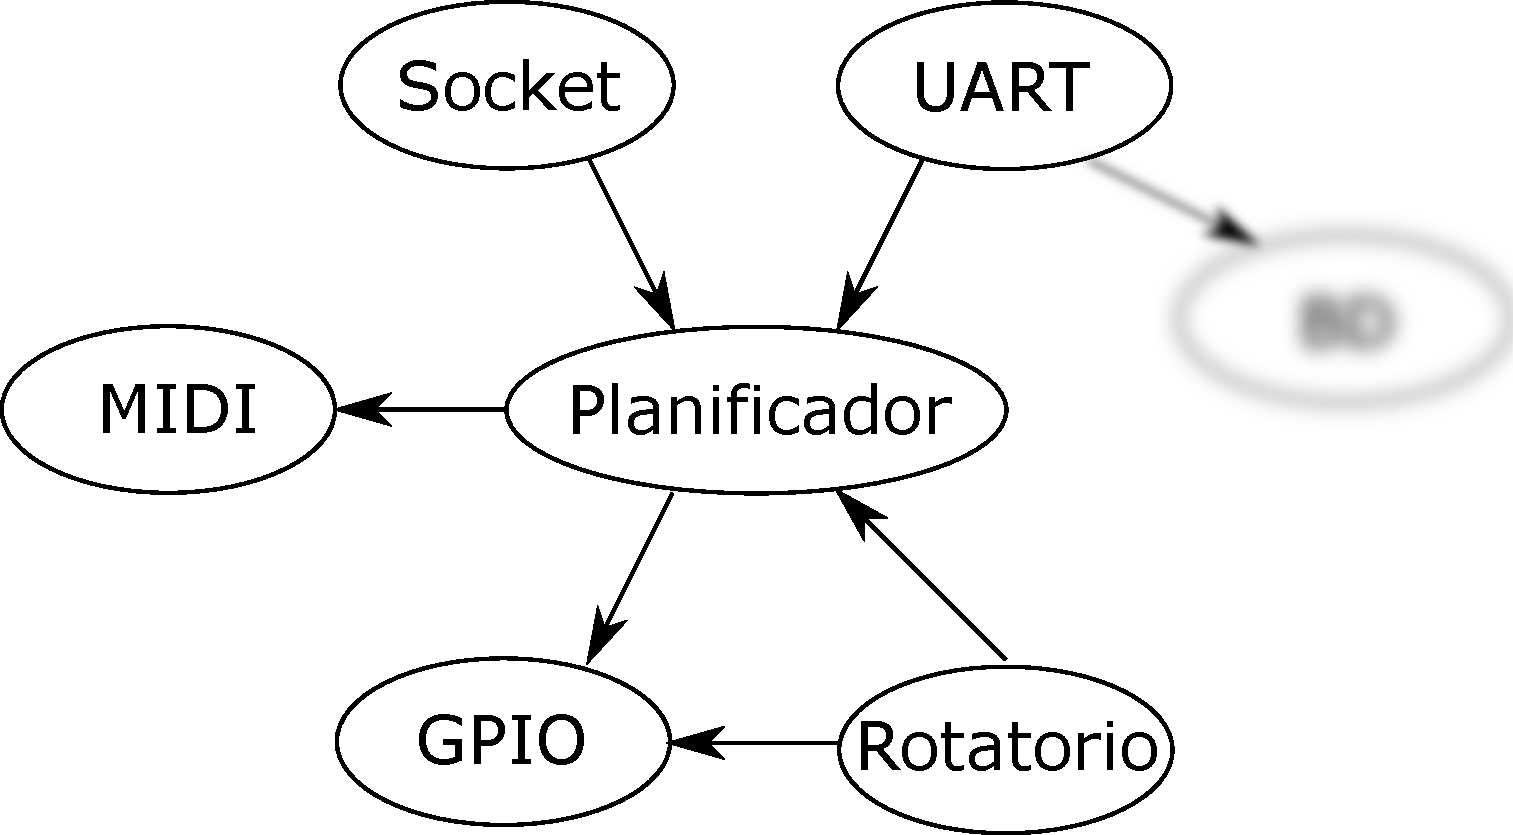
\includegraphics[width=\linewidth/2]{capitulo4/daemon_scheduler}
		\par\end{centering}
	\smallskip
	\caption{\label{fig:daemon_scheduler} Diagrama de uso del planificador.}
\end{figure} 

\smallskip

\begin{itemize}
	\item Los servidores de \textit{socket} y de \textit{UART}, y el control de interfaz reducida, envían las órdenes de control.
	\item El módulo \textit{MIDI} es utilizado para descodificar los archivos de entrada.
	\item La información extraída se dirige al módulo de salida (\textit{GPIO}) para llegar a la \textit{PCB}.
\end{itemize}

\subsection{Modo Ingeniería}

El sistema requiere un modo de mantenimiento para regular la mecánica, al que se accederá localmente, a través de una interfaz reducida que controlaremos con el codificador rotatorio y el \textit{LCD}.

El codificador permitirá acceder al modo Ingeniería, que detendrá la reproducción ---si estaba en funcionamiento--- y  aislará el planificador, ganando acceso directo a la salida \textit{GPIO}.

Vamos a diseñar la interfaz como una máquina de estados: Inicialmente el modo Ingeniería está desactivado, girando el botón se nos dará la opción de activarlo, y al pulsarlo entraremos en él. Se activará la nota más baja de la primera pista, al girar el botón podremos movernos cíclicamente por todas las notas de esa pista. Pulsando el botón cambiamos a la segunda pista, luego a la tercera, y así hasta la última. Si apretamos nuevamente el botón, volvemos al menú que nos permitirá salir del modo Ingeniería.

Este diagrama muestra las transiciones entre los estados:

\smallskip

\begin{figure}[H]
	\noindent \begin{centering}
		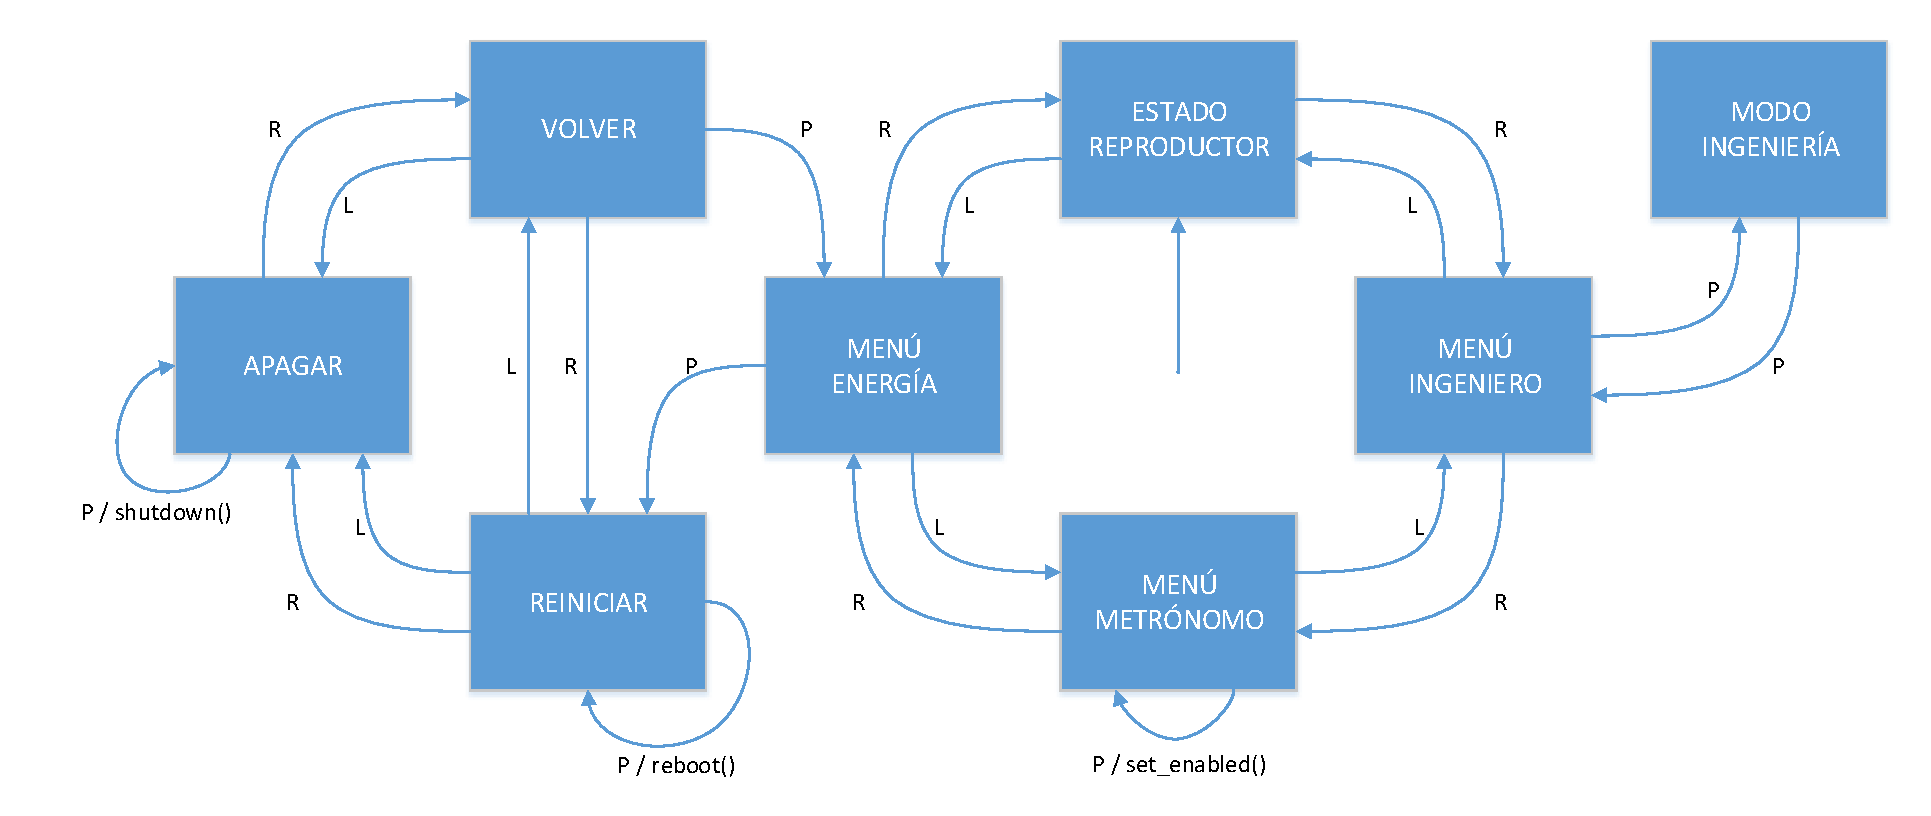
\includegraphics[width=\linewidth*3/4]{capitulo4/engineer}
		\par\end{centering}
	\smallskip
	\caption{\label{fig:engineer} Máquina de estados de la interfaz reducida.}
\end{figure} 

\smallskip

\begin{description}
	\item[OFF] Estado inicial, modo Ingeniería apagado. Mostrará el estado del reproductor.
	\item[MENU] Ofrece la opción de entrar en el modo Ingeniería.
	\item[ON] Modo Ingeniería activado, los subestados dependen de la pista y la nota actuales
\end{description}

\subsubsection{Diagrama de uso}

El módulo que controla el modo Ingeniería interacciona con el planificador, para detenerlo y aislarlo del \textit{GPIO}, y con el módulo de salida, que maneja el propio \textit{GPIO}, para manipular el estado.

\smallskip

\begin{figure}[H]
	\noindent \begin{centering}
		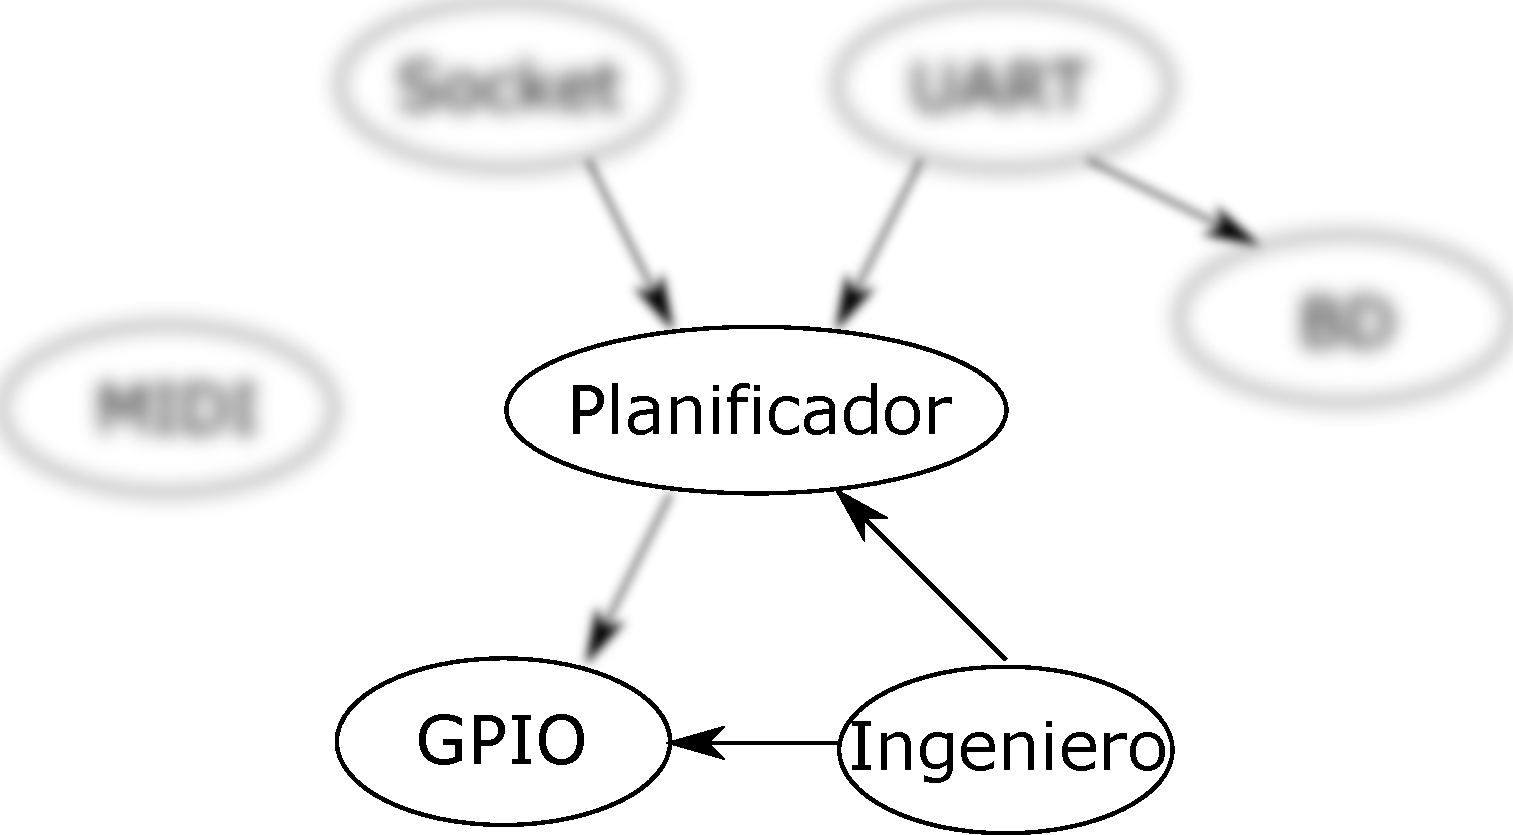
\includegraphics[width=\linewidth/2]{capitulo4/daemon_engineer}
		\par\end{centering}
	\smallskip
	\caption{\label{fig:daemon_engineer} Diagrama de uso del modo Ingeniería.}
\end{figure} 

\smallskip

\subsection{Salida hacia la PCB}

El reproductor delega en el módulo de salida las siguientes funciones:

\begin{enumerate}
	\item Dirigir las pistas de \textit{MIDI} al canal de salida correspondiente.
	\item Almacenar el estado de salida (notas pulsadas y no pulsadas).
	\item Volcar la información en el \textit{GPIO}.
\end{enumerate}

Éste será el único módulo que tendremos que cambiar a la hora de pasar de un órgano a otro. El hecho de aislar la salida también nos da flexibilidad para sustituir la interfaz \textit{GPIO} por otro tipo de salida, como la consola, con fines de mantenimiento y depuración.

Las siguientes funciones conforman la interfaz del módulo:

\begin{description}[style=nextline]
	\item[output\_init () : \textit{dword}]
	Inicializa los componentes de la salida. Devuelve 0 en caso de éxito o -1 en caso de error.
	
	\item[output\_destroy ()]
	Cierra el módulo de salida y libera la memoria ocupada.
	
	\item[output\_noteon (track, note)]
	Marcar una nota para activar en el sistema.
	
	\begin{description}
		\item[track : \textit{dword}] Índice de la pista \textit{MIDI}.
		\item[note : \textit{dword}] Número de nota \textit{MIDI}.
	\end{description}
	
	\item[output\_noteon (track, note)]
	Marcar una nota para apagarla en el sistema.
	
	\begin{description}
		\item[track : \textit{dword}] Índice de la pista \textit{MIDI}.
		\item[note : \textit{dword}] Número de nota \textit{MIDI}.
	\end{description}
	
	\item[output\_update ()]
	Vuelca el estado en la salida.
	
	\item[output\_panic ()]
	Vuelve al estado inicial (silenciar todas las notas), y lo vuelca en la salida.
	
	\item[output\_silence ()]
	Silencia todas las notas en la salida, pero mantiene el estado. Útil para pausar la reproducción.
	
\end{description}

\subsubsection{Mapeo de pistas y canales}

Nuestra especificación deja abierta la estructura que pueda tener un archivo MIDI. A pesar de que el sistema podrá descodificar \textit{MIDI} estándar, para lograr una óptima ejecución, la pieza deberá adaptarse a cada órgano concreto.

El módulo de salida permitirá asignar cada pista \textit{MIDI}, que normalmente corresponde a un pentagrama de la partitura, a un canal de salida diferente. La asignación por defecto, para el órgano estudiado, será la siguiente:

\smallskip

\begin{figure}[H]
	\noindent \begin{centering}
		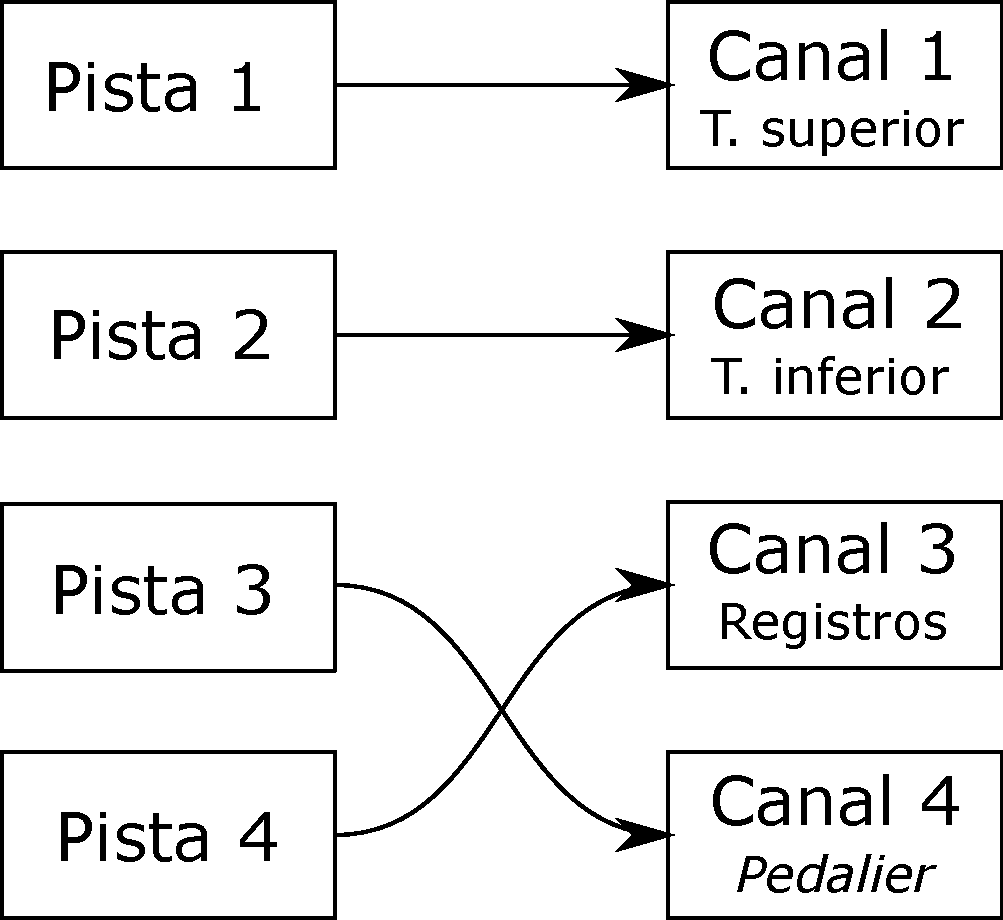
\includegraphics[width=\linewidth/3]{capitulo4/map}
		\par\end{centering}
	\smallskip
	\caption{\label{fig:map} Asignación de pistas \textit{MIDI} y canales de salida.}
\end{figure} 

\smallskip

\subsubsection{Diagrama de uso}

La interfaz de salida es utilizada principalmente por el planificador y, solo cuando éste entra en modo Ingeniería, es accedida por el módulo del mismo nombre, para poner a prueba la mecánica del sistema.

\smallskip

\begin{figure}[H]
	\noindent \begin{centering}
		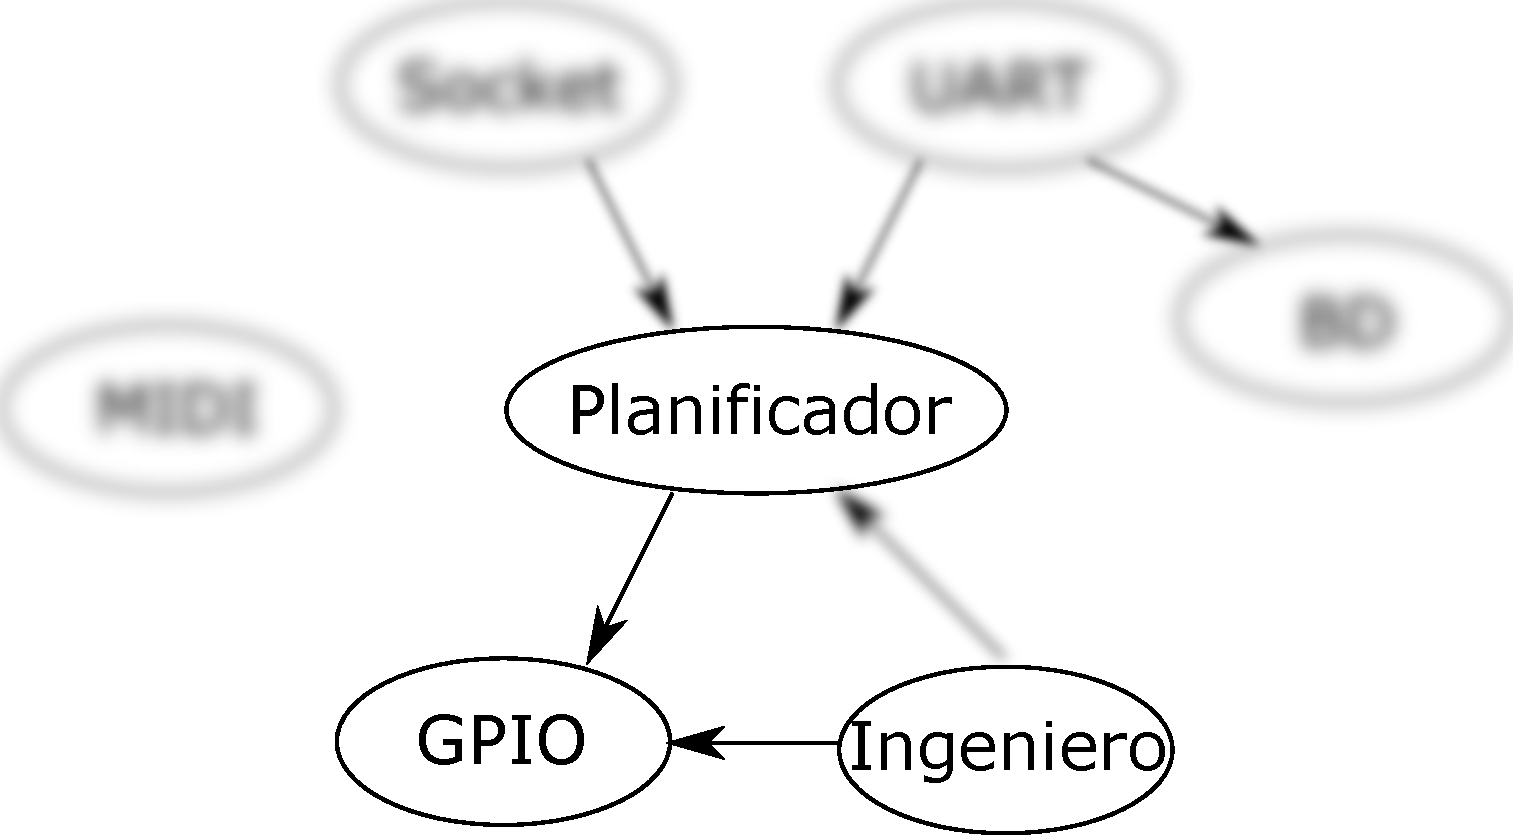
\includegraphics[width=\linewidth/2]{capitulo4/daemon_gpio}
		\par\end{centering}
	\smallskip
	\caption{\label{fig:daemon_gpio} Diagrama de uso del módulo de salida.}
\end{figure} 

\smallskip

\subsection{Seguridad}

A pesar de que el acceso al sistema se hará siempre con autentificación de usuario, nos interesa controlar que no todos los usuarios, o no todas las aplicaciones, se conecten al \textit{socket}. La seguridad de \textit{Linux} recae en gran parte sobre su sistema de archivos y permisos. Se creará un nombre de usuario de sistema para ser utilizado exclusivamente por el \textit{socket}, que tendrá permisos de lectura y escritura para dicho usuario y su grupo.

Para autorizar a un usuario a acceder al \textit{socket}, simplemente hay que añadirlo al grupo del usuario propietario.

Por otro lado, el demonio se ejecuta con permisos de \textit{superusuario}, y es inseguro mantenerse durante toda la ejecución con tales privilegios. A pesar de que introduciremos medidas de seguridad en los clientes que desarrollemos para el sistema, reduciremos los permisos después de inicializar el proceso, como medida adicional para evitar problemas.

\section{Base de datos}

La información que queremos almacenar funciona de la siguiente forma:

\begin{enumerate}
	\item Las partituras se guardan en un archivo, cuyo nombre no tiene que coincidir con el título de la partitura.
	\item De una partitura podremos conocer su duración.
	\item Una lista de reproducción es una colección de partituras, y le asignaremos un nombre.
	\item Cada partitura pertenecerá a una lista de reproducción, y solo a una.
	\item Un botón se distingue por su código, y se le asigna a una lista de reproducción, sin perjuicio de que una lista esté asignada a varios botones. Naturalmente, puede haber listas que no estén asignadas a ningún botón.
\end{enumerate}

\subsection{Modelo entidad-relación}

Atendiendo a los requisitos propuestos, modelamos nuestros datos según el siguiente diagrama:

\smallskip

\begin{figure}[H]
	\noindent \begin{centering}
		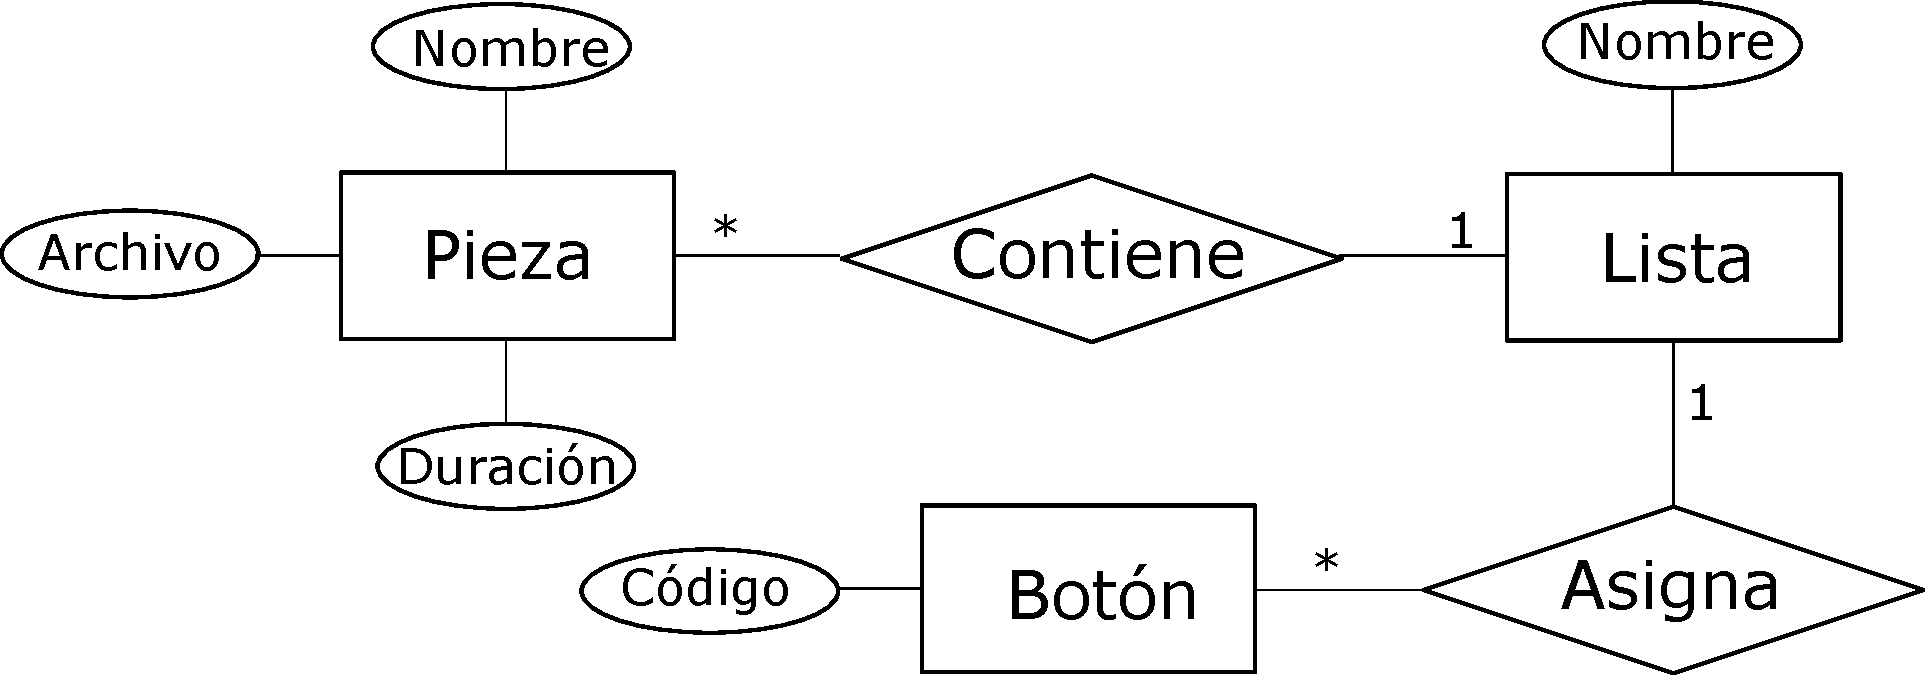
\includegraphics[width=\linewidth*3/4]{capitulo4/bd_er}
		\par\end{centering}
	\smallskip
	\caption{\label{fig:bd_er} Modelo entidad-relación.}
\end{figure} 

\smallskip

\subsection{Modelo relacional}

Una vez hemos considerado las entidades, sus atributos y las relaciones, diseñamos el modelo de datos, que depende del tipo de sistema de gestión de bases de datos ---\textit{DBMS (database management system)}--- que vayamos a utilizar. En nuestro caso, utilizaremos un \textit{DBMS} relacional.

\begin{enumerate}
	\item Convertimos en relaciones (tablas) todas las entidades y las relaciones del modelo entidad-relación.
	\item Los atributos de las entidades pasan a ser atributos de las relaciones correspondientes.
	\item Buscamos llaves candidatas y escogemos una como llave primaria. En el caso de Pieza y Lista, no tenemos llave candidata, así que añadimos un ID a cada relación.
	\item Las relaciones Contiene y Asigna tienen cardinalidad N-1, de forma que comparten la clave primaria. Fusionamos Contiene en Pieza y Asigna en Botón.
\end{enumerate}

Una vez hecho esto, el modelo resultante es el siguiente:

\smallskip

\begin{figure}[H]
	\noindent \begin{centering}
		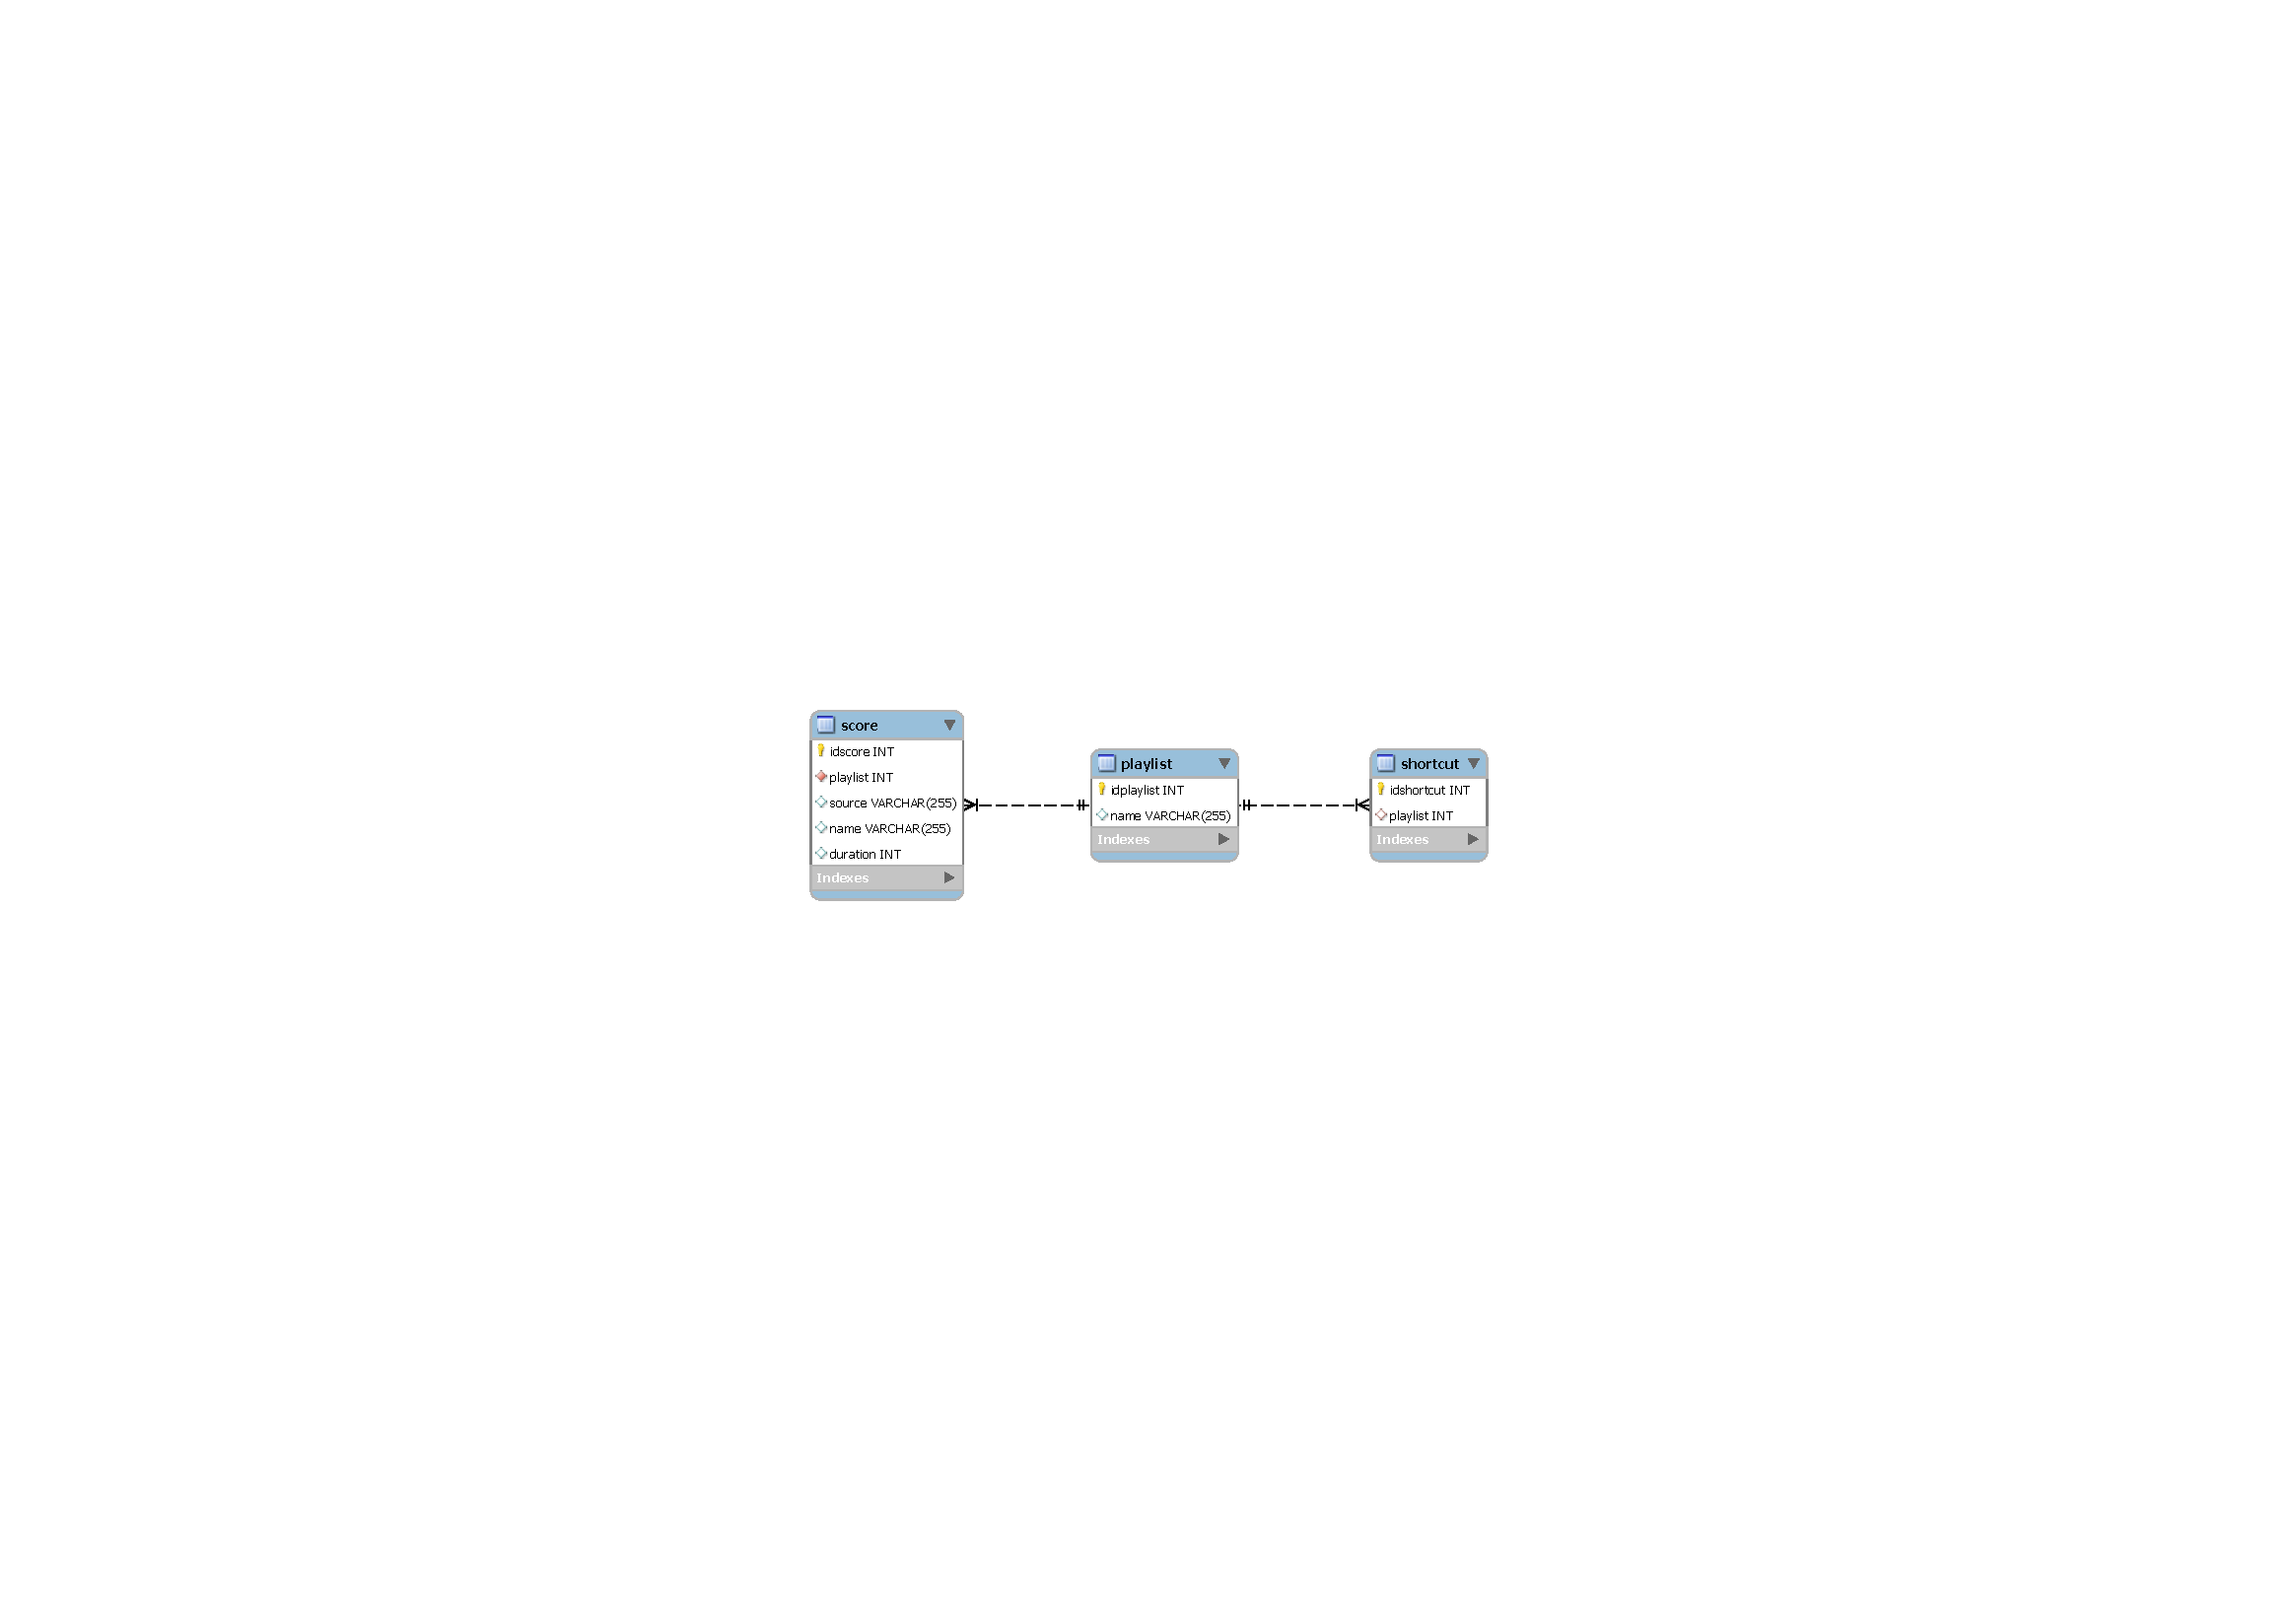
\includegraphics[clip=true, trim=390 340 390 340, width=\linewidth*3/4]{capitulo4/bd_rel}
		\par\end{centering}
	\smallskip
	\caption{\label{fig:bd_rel} Modelo relacional.}
\end{figure} 

\smallskip

\subsection{Consistencia}

Para garantizar que la base de datos mantendrá la información coherente y sin anomalías, estudiamos las relaciones para normalizarlas. Podemos verificar que nuestro modelo relacional está en 5ª forma normal, atendiendo a las siguientes condiciones:

\begin{description}
	\item[1FN] El \textit{SGBD} relacional se encarga de que se cumpla la forma normal más básica: las columnas son regulares, no habrá filas duplicadas (por la llave primaria) ni orden alguno entre filas o columnas.
	\item[2FN] Todos los atributos secundarios de cada tabla dependen de la llave primaria, por tanto, está en segunda forma normal.
	\item[3FN] No existen atributos secundarios que dependan transitivamente de la llave primaria, entonces, está en tercera forma normal.
	\item[FNBC] La forma normal de Boyce-Codd establece que los únicos determinantes sean las claves candidatas. Como el modelo está en 3FN y no existen llaves candidatas compuestas, podemos decir que está también en 3FN.
	\item[4FN] La cuarta forma normal extiende la FNBC exigiendo que no existan dependencias multivaluadas no triviales. Este modelo no tiene dependencias multivaluadas, de forma que está en 4FN.
	\item[5FN] Por último, la quinta forma normal especifica que, además de todo lo anterior, cada dependencia de unión sea implicada por claves candidatas. Esto se cumple en nuestro modelo, ya que toda llave externa se vincula a la llave primaria de otra relación.
\end{description}

Nuestro modelo relacional cumple todas las exigencias de las formas normales tenidas en cuenta, con lo que podemos garantizar que el modelo es consistente.

\smallskip

\begin{figure}[H]
	\noindent \begin{centering}
		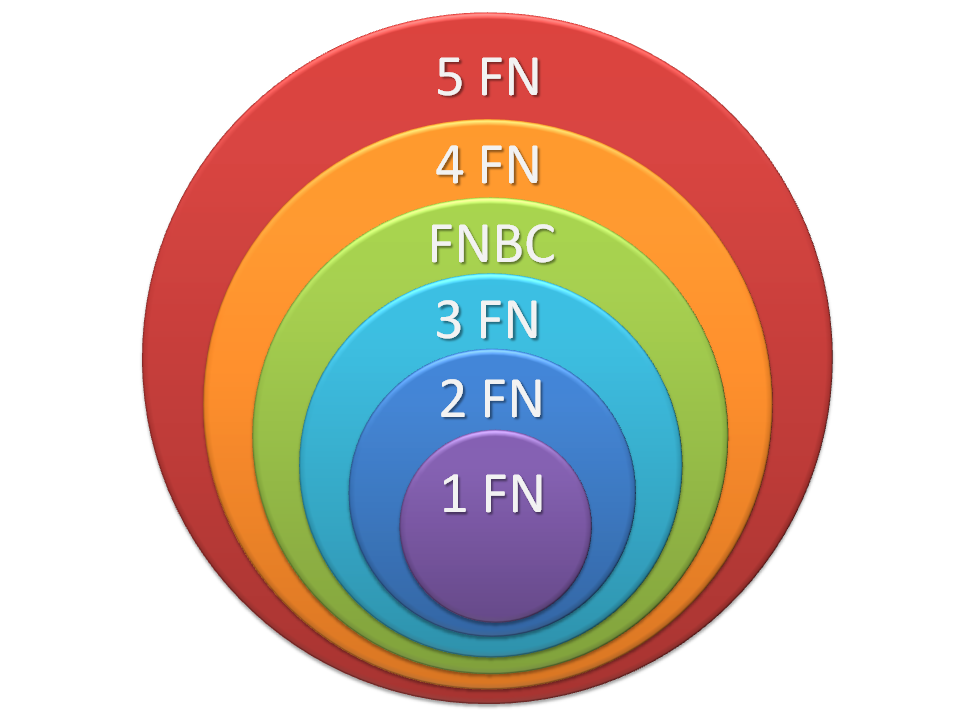
\includegraphics[width=\linewidth/2]{capitulo4/bd_fn}
		\par\end{centering}
	\smallskip
	\caption{\label{fig:bd_fn} Relación entre las formas normales.}
\end{figure} 

\smallskip

\section{Control remoto}

Hasta ahora hemos diseñado el \textit{back-end} del sistema, con todas las características que darán funcionalidad a nuestra solución. Pero aún no tenemos una interfaz que permita al usuario interactuar con el sistema, más que el control del mando a distancia o desde la \textit{PCB}.

El próximo paso es concebir el \textit{front-end} que, a tenor de los requisitos que propusimos al inicio, ofrezca al usuario la interfaz más completa posible. Frecuentemente la funcionalidad viene contrapuesta a la facilidad de uso; es nuestra tarea encontrar el mejor equilibrio posible.

Vamos a diseñar una solución enfocada al uso remoto con ayuda de un explorador de Internet, como \textit{Chrome}, \textit{Firefox} o \textit{Safari}, con lo que crearemos un servidor \textit{web}. El control del órgano queda pues estructurado de la siguiente forma:

\smallskip

\begin{figure}[H]
	\noindent \begin{centering}
		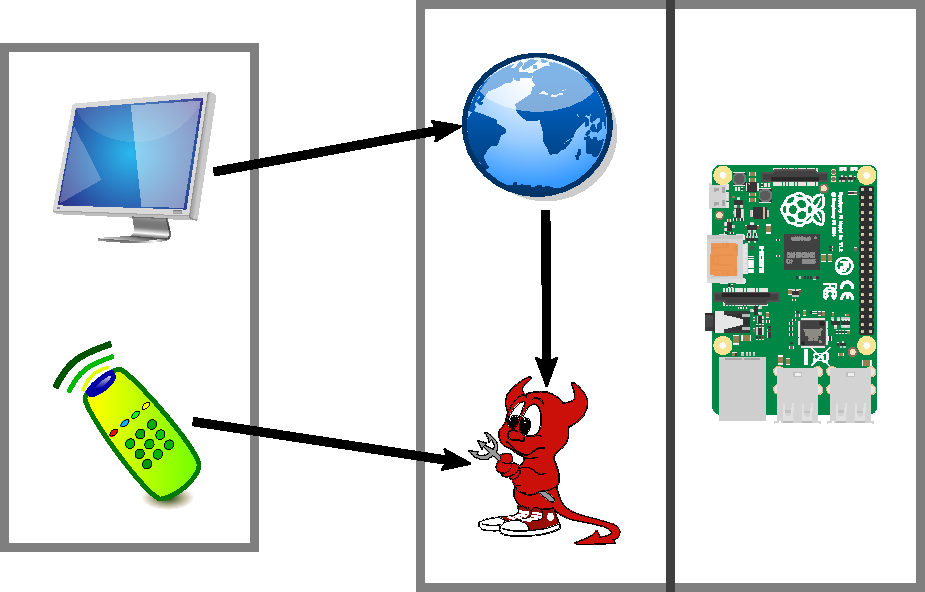
\includegraphics[width=\linewidth*2/3]{capitulo4/despliegue}
		\par\end{centering}
	\smallskip
	\caption{\label{fig:despliegue} Comunicación entre el cliente y el software del sistema.}
\end{figure} 

\smallskip

En primer lugar será especificar los casos de uso que nos enfrentarán al usuario. Después, concebiremos el aspecto de la interfaz y por último esbozaremos la estructura del diseño.

\subsection{Casos de uso}

A continuación enumeramos una relación de casos de uso que deberá cubrir la interfaz de usuario:

\begin{enumerate}
	\item Identificarse en el sistema como usuario autorizado.
	\item Salir del sistema, en el sentido de que al entrar de nuevo haya que identificarse.
	\item Controlar la reproducción directamente, a saber:
	
	\begin{enumerate}
		\item Ver el nombre de la pieza que se está reproduciendo.
		\item Ejecutar una lista de reproducción en bucle.
		\item Escoger una pieza de la lista para reproducirla.
		\item Pausar la reproducción de una pieza.
		\item Reanudar la ejecución de una pieza, si estaba pausada.
		\item Detener completamente la reproducción.
		\item Avanzar en la lista y reproducir la siguiente pieza.
		\item Retroceder en la lista y reproducir la partitura anterior.
	\end{enumerate}
	
	\item Gestionar listas de reproducción:
	
	\begin{enumerate}
		\item Crear una nueva lista, dándole un nombre.
		\item Visualizar todas las listas existentes.
		\item Modificar el nombre de la lista.
		\item Eliminar una lista.
	\end{enumerate}
	
	\item Gestionar piezas musicales:
	
	\begin{enumerate}
		\item Cargar una nueva partitura en el sistema, dentro de una lista de reproducción.
		\item Ver una relación de las piezas contenidas en una lista, y su duración.
		\item Cambiar el nombre de una pieza.
		\item Borrar una pieza del sistema.
	\end{enumerate}
	
	\item Gestionar asignaciones de botones del mando:
	
	\begin{enumerate}
		\item Ver las asignaciones actuales.
		\item Cambiar la lista a reproducir cuando se pulsa un botón, escogiéndola entre todas las listas.
	\end{enumerate}
	
	\item Controlar básicamente la energía del sistema:
	
	\begin{enumerate}
		\item Apagar el sistema.
		\item Reiniciar el sistema.
	\end{enumerate}
	
	\item Escoger el idioma en que se muestra el texto, entre una lista de lenguas disponibles.
\end{enumerate}

\subsection{Modelo-vista-controlador}

Para estructurar los elementos que conformarán la interfaz, utilizaremos el patrón de modelo-vista-controlador, que divide la funcionalidad de un sistema en tres bloques, con el siguiente criterio:

\smallskip

\begin{figure}[H]
	\noindent \begin{centering}
		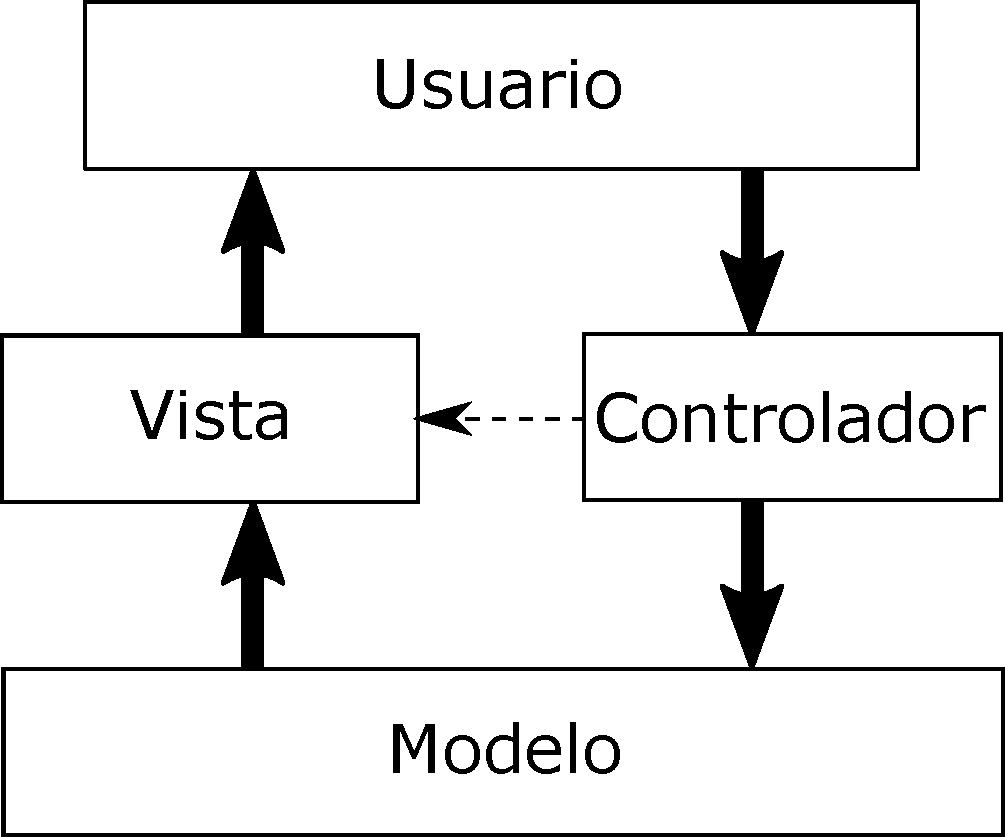
\includegraphics[width=\linewidth/2]{capitulo4/mvc}
		\par\end{centering}
	\smallskip
	\caption{\label{fig:mvc} Relación entre la vista, el modelo y el controlador.}
\end{figure} 

\smallskip

\begin{description}
	\item[Vista] Reúne los elementos que van a proporcionar al usuario la información que requiere.
	\item[Controlador] Comprende los módulos a los que el usuario acudirá para manipular el sistema. Eventualmente, después de realizar una operación, puede llamar a la vista para realimentar de información al usuario. 
	\item[Modelo] Contiene los componentes más internos, abstrayendo a la vista y al controlador de la representación de los datos o la interacción con el sistema.
\end{description}

Considerando los casos de uso y los requisitos, hemos enmarcado en el esquema modelo-vista-controlador los siguientes elementos:

\smallskip

\begin{figure}[H]
	\noindent \begin{centering}
		\includegraphics[width=\linewidth*2/3]{capitulo4/mvc_completo}
		\par\end{centering}
	\smallskip
	\caption{\label{fig:mvc_completo} Módulos que componen el sistema.}
\end{figure} 

\smallskip

A lo largo de esta sección detallaremos el comportamiento de todos los componentes.

\subsection{Estilo de la interfaz}

La visualidad es un punto importante en el diseño de interfaces gráficas, es la encargada de proporcionar una experiencia de usuario y hacer asequible la utilización del sistema. Pretendemos entregar la información requerida de forma clara y concisa, disponer fácilmente de los controles que puedan ser necesarios en cada vista, y que el estilo sea agradable y acorde a la solución que se está diseñando.

Por ello, vamos a fijarnos en la guía de estilo \textit{Material Design} de \textit{Google} para inspirarnos. La idea es sencilla: cada elemento de la interfaz se entiende como una hoja de papel. El diseñador maquetará la interfaz en base a hojas que se solapan, produciendo una sutil sombra cuando esto ocurre.

\textit{Material design} provee una gran cantidad de componentes de control y paletas de colores. De todos ellos, escogeremos listas, menús desplegables y botones flotantes. Nos decantamos por un color marrón, que evoca tranquilidad y estabilidad, dando idea de un \textit{software} intuitivo y robusto.

Una vez dibujados los primeros trazos, no es necesario maquetar completamente la interfaz con una aplicación para manipular imágenes, pudiendo diseñar las vistas en \textit{HTML} y \textit{CSS}, aún sin código de programación. Pero es muy útil dibujar al menos una página que nos sirva de plantilla. La siguiente imagen es una primera versión de la maqueta, diseñada con \textit{Adobe Photoshop}:

\smallskip

\begin{figure}[H]
	\noindent \begin{centering}
		\includegraphics[width=\linewidth*3/4]{capitulo4/maqueta}
		\par\end{centering}
	\smallskip
	\caption{\label{fig:maqueta} Maquetación de las capas.}
\end{figure}

\smallskip

\subsection{Portada}

La portada es la vista principal y va a cumplir dos funciones:

\begin{enumerate}
	\item Presentar la aplicación y dar la bienvenida.
	\item Introducir una contraseña para acceder al sistema.
\end{enumerate}

La vista proporcionará un fondo dinámico, con varias imágenes temáticas, y un cuadro para introducir la contraseña. Al hacerlo, se enviará al controlador, que se ocupará de verificar que la clave es correcta y concederá el acceso al reproductor.

\subsubsection{Autentificación}

El módulo de autentificación recibe la contraseña introducida por el usuario, y utiliza la interfaz del modelo para validarla.

La contraseña será la de un usuario (a especificar) del sistema Linux, que provee una forma segura de almacenar contraseñas cifradas y gestionar usuarios. La verificación no se hará directamente, sino que llamaremos a un programa externo, que describiremos más abajo, para que haga tal trabajo.

El resto de vistas y controladores de la interfaz deberán consultar si se ha iniciado sesión antes de proceder a realizar la petición correspondiente. Cuando un usuario accede al sistema con una contraseña válida, se guardará una marca en su sesión para no tener que introducirla en cada vista.

Definiremos las siguientes funciones:

\begin{description}[style=nextline]
	\item[login (password)]
	Comprueba la contraseña llamando a una aplicación que diseñaremos específicamente.
	
	\begin{description}
		\item[password] Clave introducida por el usuario.
	\end{description}
	
	Si la contraseña es correcta, marca la autorización en la sesión y redirige a la vista del Reproductor. Si no, redirige a la portada y muestra un mensaje de error.
	
	\item[logout ()]
	Cierra la sesión retirando la marca de autorización de la sesión. Redirige a la portada.
	
\end{description}

A continuación mostramos el diagrama de uso de la vista de portada y el módulo de acceso:

\smallskip

\begin{figure}[H]
	\noindent \begin{centering}
		\includegraphics[width=\linewidth/2]{capitulo4/mvc_acceso}
		\par\end{centering}
	\smallskip
	\caption{\label{fig:mvc_acceso} Módulos implicados en el acceso al sistema.}
\end{figure} 

\smallskip

\subsection{Reproductor}

El reproductor es la parte fundamental de la interfaz. Mostrará los siguientes elementos:

\begin{enumerate}
	\item Estado del demonio (reproduciendo, pausado o detenido).
	\item Nombre de la pieza que se está ejecutando (si procede).
	\item Lista de reproducción activa (si procede).
	\item Controles de reproducción:
	
	\begin{enumerate}
		\item Pausar.
		\item Reanudar.
		\item Detener.
		\item Siguiente pieza.
		\item Pieza anterior.
	\end{enumerate}
\end{enumerate}

Hay que tener en cuenta que el protocolo de comunicación establece que el reproductor del demonio no es consciente de la lista de reproducción en la base de datos. Al ordenar una reproducción se le envía los nombres de archivo, como se describe en la función \textit{player\_playlist()} del demonio. De igual forma, al consultar el estado, devuelve el nombre de la pieza que se está ejecutando, cuya lista se puede conocer por reunión natural en la base de datos, y si no se encuentra, es porque se está reproduciendo un archivo externo, o tal vez otro usuario la ha eliminado.

Esto se hace así para evitar mantener un estado común entre el demonio y la interfaz, que podría provocar incoherencias si el cliente se desconecta repentinamente o si hay varios usuarios conectados al mismo tiempo.

Se definirán las siguientes funciones:

\begin{description}[style=nextline]
	\item[play (idplaylist, idscore)]
	Reproduce en bucle la lista indicada, empezando por la pieza especificada.
	
	\begin{description}
		\item[idplaylist] ID de la lista en la base de datos.
		\item[idscore] (opcional) ID de la primera pieza a reproducir.
	\end{description}
	
	Redirige a la vista del Reproductor.
	
	\item[pause ()]
	Pausa la reproducción de la partitura.
	
	\item[resume ()]
	Reanuda la ejecución de la pieza.
	
	\item[stop ()]
	Detiene completamente la reproducción en el demonio.
	
\end{description}

El reproductor interacciona con el resto de la interfaz según este esquema:

\smallskip

\begin{figure}[H]
	\noindent \begin{centering}
		\includegraphics[width=\linewidth/2]{capitulo4/mvc_reproductor}
		\par\end{centering}
	\smallskip
	\caption{\label{fig:mvc_reproductor} Módulos implicados en el reproductor.}
\end{figure} 

\smallskip

\subsection{Gestión de listas de reproducción}

Una parte importante de la interfaz es facilitar la organización de la información. Las piezas musicales se clasificarán en listas de reproducción. Este módulo agrega la funcionalidad necesaria para gestionar listas.

El gestor se presentará con los siguientes controles:

\begin{enumerate}
	\item Lista de listas de reproducción, con el siguiente contenido:

	\begin{enumerate}
		\item Nombre de la lista.
		\item Número de piezas contenidas.
		\item Vínculo para acceder a la lista.
		\item Vínculo para ejecutar la lista en el reproductor.
	\end{enumerate}
	
	\item Botón para crear una nueva lista. Al dispararlo, abrirá un cuadro de diálogo para introducir el nombre de la lista.
	
\end{enumerate}

El controlador tendrá las siguientes funciones:

\begin{description}[style=nextline]
	\item[new\_playlist (name)]
	Genera una lista nueva, con el nombre que se recibe. 
	
	\begin{description}
		\item[name] Nombre que identificará a la nueva lista.
	\end{description}
	
	Redirige al administrador de la nueva lista.
	
	\item[rename\_playlist (idplaylist, name)]
	Cambia el nombre de una lista existente.
	
	\begin{description}
		\item[idplaylist] ID de la lista en la base de datos.
		\item[name] Nuevo nombre a asignar a la lista.
	\end{description}
	
	Redirige al administrador de la lista.
	
	\item[delete\_playlist (idplaylist)]
	Elimina una lista de reproducción y todas las partituras que contenga.
	
	\begin{description}
		\item[idplaylist] ID de la lista en la base de datos.
	\end{description}
	
	Redirige al gestor de listas de reproducción.
	
\end{description}

Los componentes implicados en la gestión de listas se relacionan de la siguiente forma:

\smallskip

\begin{figure}[H]
	\noindent \begin{centering}
		\includegraphics[width=\linewidth/2]{capitulo4/mvc_listas}
		\par\end{centering}
	\smallskip
	\caption{\label{fig:mvc_listas} Módulos implicados en el gestor de listas.}
\end{figure} 

\smallskip

\subsection{Gestión de partituras}





\subsection{Asignación del mando a listas}

\subsection{Control de energía}

\subsection{Soporte de idiomas}

\subsection{Navegación}

\subsection{Sesión}

\subsection{Comunicación con el demonio}

\subsection{Comunicación con la base de datos}

\section{Protocolo entre el control y el demonio}

\section{Aplicaciones auxiliares}

\subsection{Terminal del reproductor}

\subsection{Información de archivo MIDI}

\subsection{Comprobación de contraseña}

\clearpage{\cleardoublepage}
\clearpage{\pagestyle{empty}\cleardoublepage}
%
\chapter{Implementación del sistema.}
\label{cap: capitulo_5}

A lo largo de este capítulo vamos a explicar cómo hemos llevado a cabo el proceso de implementación del sistema, partiendo del diseño especificado en las páginas anteriores.

Todos los bloques se han implantado con una filosofía similar, teniendo en cuenta que nos dirigimos a un \textbf{sistema empotrado}, de prestaciones limitadas, y donde la \textbf{seguridad} y el \textbf{tiempo de respuesta} son cruciales.

Debemos tener también en cuenta que el servicio podrá ser utilizado por \textbf{varios usuarios} a la vez ---incluso varios componentes--- y el planificador, si bien no requiere características de tiempo-real estricto, es necesario que responda adecuadamente a los tiempos marcados por la partitura.

En el demonio, nuestra máxima prioridad será la \textbf{eficiencia}, mientras que en la interfaz \textit{web} nos centraremos en la \textbf{accesibilidad}.

\section{Planificación}

En base a nuestro objetivo final, este proyecto está estrechamente relacionado con el de Mikel Aguayo Fernández, que abordará la parte relacionada con \textit{hardware}.

Nuestro diseño es genérico para cualquier órgano pero \textbf{específico para la plataforma} \textit{hardware}. Por tanto, hay una parte del sistema que no se puede diseñar hasta conocer el proyecto de la \acrshort{PCB}. Para realizar una correcta planificación es necesario tener en cuenta qué parte de nuestro diseño depende del de Mikel Aguayo.

\subsection{Dependencias entre tareas}

Esencialmente tenemos los siguientes puntos en común:

\begin{enumerate}
	\item Compartimos inicialmente los \textbf{requisitos}, para entonces clasificarlos entre nuestros proyectos.
	\item El otro proyecto necesita el \textbf{análisis} realizado sobre el órgano.
	\item El nuestro, a su vez, depende del \textbf{diseño} que se haga de la \acrshort{PCB}.
	\item La \textbf{verificación} vuelve a poner en común nuestros trabajos.
\end{enumerate}

La siguiente figura descompone a \textit{grosso modo} las tareas e ilustra las \textbf{dependencias} encontradas:

\smallskip

\begin{figure}[H]
	\noindent \begin{centering}
		\includegraphics[width=\linewidth*3/4]{capitulo5/planificacion}
		\par\end{centering}
	\smallskip
	\caption{\label{fig:planificacion} Diagrama de dependencia de tareas.}
\end{figure} 

\smallskip

Esto significa que la \textbf{planificación temporal} de las tareas se esbozará de la siguiente forma:

\smallskip

\begin{figure}[H]
	\noindent \begin{centering}
		\includegraphics[clip=true,trim=50 420 50 50,width=\linewidth*3/4]{capitulo5/plan_gantt}
		\par\end{centering}
	\smallskip
	\caption{\label{fig:plan_gantt} Diagrama de Gantt básico.}
\end{figure} 

\smallskip

\subsection{Planificación prevista}

Conocidas las tareas básicas a realizar, proponemos la siguiente planificación para todos los bloques a desarrollar en el sistema. Hemos asignado principalmente las tareas por \textbf{semanas}, aunque algunas de ellas se podrán hacer en común por su simplicidad, y otras deberemos \textbf{descomponerlas} en prototipo e implementación final.

\smallskip

\begin{figure}[H]
	\noindent \begin{centering}
		\includegraphics[clip=true,trim=20 50 50 50,width=\linewidth]{capitulo5/gantt}
		\par\end{centering}
	\smallskip
	\caption{\label{fig:gantt} Diagrama de Gantt para planificación.}
\end{figure} 

\smallskip

Como podemos ver, el primer paso es \textbf{analizar} el funcionamiento y la mecánica del órgano para permitir a Mikel continuar su trabajo. Mientras él diseña la \acrshort{PCB}, nosotros comenzamos el \textbf{diseño} de los módulos que no dependen de ésta. Tan pronto como recibamos su diseño, podremos desarrollar el resto del sistema.

\section{Servicio del reproductor}

Este bloque compone el \textit{back-end} del sistema. Comprende una gran cantidad de elementos técnicos y hace uso de numerosas funciones del sistema operativo. Vamos a escribirlo casi por completo en \textbf{lenguaje C}, por las siguientes razones:

\begin{enumerate}
	\item Alta calidad y \textbf{eficiencia}.
	\item Cercanía al \textbf{\textit{hardware}}.
	\item Capacidad para hacer \textbf{llamadas al sistema} Linux.
	\item Posibilidad de acceder al código ensamblador para hacer \textbf{optimizaciones}.
\end{enumerate}

Aunque todos los ejecutables se van a compilar desde código \textit{C}, haremos uso de \textit{shell-scripts} y un \textit{Makefile} que nos permitirá compilar fácilmente las fuentes e instalar los ejecutables.

En ciertos componentes, necesitaremos hacer \textbf{prototipos} para estudiar su funcionamiento y realizar pruebas de concepto, antes de implantarlos definitivamente. Esto lo haremos en \textbf{Python}, un lenguaje interpretado y de programación más ágil que C.

En resumen, utilizaremos el siguiente procedimiento con los componentes más complejos, que así lo requieran:

\smallskip

\begin{figure}[H]
	\noindent \begin{centering}
		\includegraphics[width=\linewidth/2]{capitulo5/prototipado}
		\par\end{centering}
	\smallskip
	\caption{\label{fig:prototipado} Esquema de prototipado.}
\end{figure} 

\smallskip

El código hace uso de los siguientes componentes externos:

\begin{enumerate}
	\item Biblioteca estándar de C \cite{cplusplus}.
	\item Interfaz \acrshort{POSIX} \cite{wiki_posix}.
	\item Llamadas al sistema Linux \cite{manpages}.
	\item Sistema de archivos especial \textit{GPIOFS} \cite{gpiofs}.
	\item \acrshort{API} para C del cliente MySQL (para el módulo de base de datos) \cite{mysql}.
	\item Biblioteca \textit{WiringPi} (solo para el modo Ingeniería) \cite{wiringpi}.
	\item Biblioteca estándar de Python (para los prototipos) \cite{python}.
\end{enumerate}

\subsection{Descodificador de MIDI}

Este fue el primer módulo a implementar. Estudiado el análisis, el diseño es sencillo por la independencia entre eventos. Sin embargo, la implementación presentaba una \textbf{complejidad} notable, sobre todo porque no hay un carácter separador entre eventos, y tanto los meta-eventos como las marcas de duración tienen \textbf{longitud variable}.

Como ya indicamos en la sección \ref{sec:fmto_midi}, el protocolo \acrshort{MIDI} especifica que los valores numéricos se indican en \textit{big-endian}. Como el procesador del \textit{Raspberry} funciona en \textit{little-endian}, hay que \textbf{intercambiar los \textit{bytes}} de los números que ocupen más de un \textit{byte}. La figuras siguientes ilustran este problema:

\smallskip

\begin{figure}[H]
	\noindent \begin{centering}
		\includegraphics[width=\linewidth/3]{capitulo5/big_endian}
		\includegraphics[width=\linewidth/3]{capitulo5/little_endian}
		\par\end{centering}
	\smallskip
	\caption[Big-endian y little-endian]{\label{fig:endianness} Big-endian (izquierda) y little-endian (derecha). \cite{wiki_endianness}}
\end{figure}
	
\smallskip

Por otro lado, también sabemos que ciertos valores, como el \textit{delta} de cada evento o el tamaño de datos de los meta-eventos, son de \textbf{longitud variable}: cada \textit{byte} tiene un significando de 7 \textit{bits}, los menos significativos. Mientras el último \textit{bit} sea 1, entonces el \textit{byte} siguiente del archivo corresponde, de igual forma, a otros 7 \textit{bits}, que se colocarían a la derecha (menos significativos).

\smallskip

\begin{figure}[H]
	\noindent \begin{centering}
		\includegraphics[width=\linewidth/2]{capitulo5/varlen}
		\par\end{centering}
	\smallskip
	\caption{\label{fig:varlen} Campo de longitud variable.}
\end{figure}

\smallskip

Además, podemos ver que todos los tipos de evento se numeran a partir de $80_{16}$, o sea, su \textit{bit} más significativo es 1. Si el analizador buscara un tipo de evento y encontrara un valor por debajo de este número, significa que el archivo está \textbf{obviando el tipo} de evento, y está indicando los parámetros ---cuyo tope es 127---.

\subsubsection{Prototipo}

En primer lugar hacemos una implementación sencilla en Python, que nos permita comprobar que hemos aplicado correctamente los conceptos.

Todos los valores de los tipos enumerados se hacen mediante constantes. Tal como dicta el diseño, la clase principal es \code{MidiFile}, que recibe un nombre de archivo. Los métodos se han implementado de la siguiente forma:

\begin{description}[style=nextline]
	\item[\code{\_\_init\_\_(self, pathname)}]
	Constructor: crea un archivo \acrshort{MIDI} completo desde un nombre de archivo (\code{pathname}). Abre el archivo, desempaqueta la cabecera y escribe los atributos del objeto en consecuencia. A continuación, inicializa la lista de pistas llamando al constructor de \code{MidiTrack} tantas veces como pistas indica el archivo.
	
	\item[\code{\_\_len\_\_(self)}]
	Devuelve el tamaño de la lista de pistas.
	
	\item[\code{\_\_getitem\_\_(self, key)}]
	Devuelve la pista indicada (\code{key}).
	
\end{description}

De esta forma, un archivo es sustancialmente una lista de pistas, y define los siguientes métodos:

\begin{description}[style=nextline]
	\item[\code{\_\_init\_\_(self, file)}]
	Constructor: crea una pista a partir de un fichero abierto (\code{file}), cuyo puntero debe estar al inicio de una nueva pista. Análogamente al constructor de \code{MidiFile}, analiza la cabecera, comprueba que sea válida y genera una lista de eventos utilizando para ello \code{MidiEvent.parseEvent()}
	
	\item[\code{\_\_iter\_\_(self)}]
	Permite iterar sobre los eventos la pista, devolviendo un iterador de la lista de eventos.	
\end{description}

Otra de las clases a implementar es \code{MidiEvent}, que representa cada uno de los eventos contenidos en un archivo, y contiene los siguientes métodos:

\begin{description}[style=nextline]
	\item[\code{\_\_init\_\_(self, delta, value, param1, param2)}]
	Constructor: crea un evento \acrshort{MIDI}, copiando en el sujeto (\code{self}) el retardo temporal (\code{delta}), el tipo de evento, junto al canal (\code{value}) y los parámetros (\code{param1} y \code{param2}).
	
	\item[\code{\_\_repr\_\_(self)}]
	Devuelve una cadena que expresa la representación del objeto, de la siguiente forma:
	
	\begin{center}
		<delta>: Event <tipo>@<canal> ( <Parámetro 1>, <Parámetro 2> )
	\end{center}
	
	\item[\code{note(self)}]
	Devuelve el código de nota (primer parámetro).
	
	\item[\code{velocity(self)}]
	Devuelve la intensidad sonora (primer parámetro).
	
	\item[\code{aftertouch(self)}]
	Devuelve la variación de intensidad, sita en el segundo parámetro si el tipo es \code{NOTE\_AFTERTOUCH} o en el primero en otro caso.
	
	\item[\code{controller(self)}]
	Devuelve el número de controlador (primer parámetro).
	
	\item[value\code{(self)}]
	Devuelve el valor del controlador (segundo parámetro).
	
	\item[program\code{(self)}]
	Devuelve el código de programa (primer parámetro).
	
	\item[pitch\code{(self)}]
	Devuelve el valor del \textit{pitch-bend} uniendo los parámetros:
	
	\begin{center}
		$p_1 \; | \; (p_2 << 7)$
	\end{center}
	
	\item[parseEvents(file)]
	Método de clase. Analiza todos los eventos de la pista actual en el archivo (\code{file}) hasta encontrar el meta-evento \code{END\_OF\_TRACK}. Su funcionamiento es el siguiente:
	
	\smallskip
	
	\begin{figure}[H]
		\noindent \begin{centering}
			\includegraphics[width=\linewidth*2/3]{capitulo5/flujo_parser}
			\par\end{centering}
		\smallskip
		\caption{\label{fig:flujo_parser} Diagrama de flujo del analizador.}
	\end{figure}
	
	\smallskip
	
	\item[\code{varlen(file)}]
	Es una función auxiliar privada que recibe el archivo (\code{file}) apuntando a un campo de longitud variable (véase la figura \ref{fig:varlen}) y devuelve su valor.
	
\end{description}

Por último, la clase \code{MetaEvent} hereda de \code{MidiEvent} y, de acuerdo al diseño, tiene los siguientes métodos:

\begin{description}[style=nextline]
	\item[\code{\_\_init\_\_(self, delta, evtype, data)}]
	Constructor. Crea un metaevento copiando en el sujeto (\code{self}) el retardo temporal (\code{delta}), el tipo de meta-evento (\code{evtype}) y la cadena de datos (\code{data}).
	
	\item[\code{\_\_repr\_\_(self)}]
	Devuelve una cadena que expresa la representación del objeto, de la siguiente forma:
	
	\begin{center}
		<delta>: Meta-event <tipo>@<canal> ( <Parámetro 1>, <Parámetro 2> )
	\end{center}
	
	\item[\code{number(self)}]
	Devuelve el número de secuencia (primer \textit{byte} de la cadena).
	
	\item[\code{text(self)}]
	Devuelve la propia cadena de texto.
	
	\item[\code{channel(self)}]
	Devuelve el canal por defecto (primer \textit{byte} de la cadena).
	
	\item[\code{tempo(self)}]
	Calcula el \textit{tempo} en \textit{$\mu s / \quarternote$}. Este valor ocupa 3 \textit{bytes}, que se acuñan así:
	
	\begin{center}
		($d_0 << 16) \; | \; (d_1 << 8) \; | \; d_2$
	\end{center}
	
	\item[\code{offset(self)}]
	Devuelve el desplazamiento temporal en una lista con el siguiente contenido:
	
	\begin{enumerate}
		\item Velocidad, según los 2 \textit{bits} más significativos del primer \textit{byte} de la cadena:
		
		\begin{itemize}
			\item $d_0[7:6] = 0 \Rightarrow 24 \; fps$
			\item $d_0[7:6] = 1 \Rightarrow 25 \; fps$
			\item $d_0[7:6] = 2 \Rightarrow 30 \; fps$
		\end{itemize}

		\item Número de horas ($d_0[5:0]$).
		\item Número de minutos ($d_1$).
		\item Número de segundos ($d_2$).
		\item Número de cuadros ($d_3$).
	\end{enumerate}

	\item[\code{time(self)}]
	Devuelve la marca de compás en una lista, de la siguiente forma:
	
	\begin{enumerate}
		\item Numerador: $d_0$.
		\item Denominador: $2^{d_1}$.
		\item Número de \textit{ticks} entre cada marca del metrónomo: $d_2$.
		\item Subdivisión, en \textit{fusas / click}: $d_3$.
	\end{enumerate}
	
	\item[\code{key(self)}]
	Devuelve la tonalidad en una lista, con los siguientes valores:
	
	\begin{enumerate}
		\item Número de $\sharp$ si es positivo, o número de $\flat$ si es negativo: $d_0$.
		\item Modo: $d_1$
	\end{enumerate}
\end{description}

Ya que es una prueba de concepto, el analizador emitirá un \textit{log} con  todos los datos extraídos de un archivo. Un ejemplo de salida es el siguiente:

\smallskip

\begin{figure}[H]
	\noindent \begin{centering}
		\includegraphics[width=\linewidth/2]{capitulo5/cap_parser}
		\par\end{centering}
	\smallskip
	\caption{\label{fig:cap_parser} Salida del prototipo del analizador.}
\end{figure}

\smallskip

\subsubsection{Implementación final}

Una vez puesto a prueba el analizador de \acrshort{MIDI} en Python, lo pasamos a C. Al ser un lenguaje no orientado a objetos, hay que introducir algunos cambios, pero el algoritmo es el mismo que el del prototipo. 

Sin embargo, las funciones no diferirán mucho del lenguaje anterior, porque en Python hay que poner el \textbf{sujeto} del método como primer parámetro, y en la nueva implementación haremos lo mismo. La diferencia más significativa es que tendremos que insertar un \textbf{destructor}.

En primer lugar, definimos los \textbf{tipos enumerados}:

\begin{description}
	\item[\code{enum format\_t}] Formato del archivo:
	
	\begin{description}
		\item[\code{SINGLE\_TRACK}] Una sola pista.
		\item[\code{MULTIPLE\_INDEPENDENT}] Varias pistas, simultáneas.
		\item[\code{MULTIPLE\_SIMULTANEOUS}] Varias pistas, independientes.
	\end{description}
	
	\item[\code{enum division\_t}] Unidad de medida de la división de tiempo:
	
	\begin{description}
		\item[TICKS\ PER\ BEAT] La división se especifica en \textit{ticks}/\quarternote.
		\item[FRAMES\_PER\_SECOND] La división se especifica en \textit{ticks/fotograma}.
	\end{description}
	
	\item[\code{enum midievent\_type\_t}] Tipo de evento \acrshort{MIDI}. Se enumeran en la tabla \ref{tab:midi_eventos}.
	\item[\code{enum metaevent\_type\_t}] Tipo de meta-evento. Se enumeran en la tabla \ref{tab:midi_metaeventos}.
	
	\item[\code{enum midimode\_t}] Modo tonal:
	
	\begin{description}
		\item[MAJOR] Modo mayor.
		\item[MINOR] Modo menor.
	\end{description}
\end{description}

Aparte del resto de transformaciones obvias, en pro de la velocidad de ejecución, hacemos los siguientes cambios:

\begin{enumerate}
	\item Anteponemos un \textbf{prefijo} a las funciones propias de cada estructura. El primer parámetro de todas ellas será un puntero a la misma.
	
	\item Eliminamos las funciones de consula que acceden llanamente a los parámetros, y a cambio sustituimos los parámetros simples por \textbf{uniones} con los nombres de las funciones.
	
	\item Ya que no podemos conocer a \textit{priori} el número de eventos que contendrá una pista, vamos a interpretar la composición propuesta por el diagrama \ref{fig:uml_midi} como una \textbf{lista enlazada} de eventos. Ya que la inserción y la lectura van a ser secuenciales, garantizamos una eficiencia algorítmica $O(1)$ en cada acceso.
\end{enumerate}

\subsection{Planificador}
\label{subsec:impl_planificador}

El planificador es la parte más crítica del sistema: debe cronometrar y ejecutar los eventos del archivo que está abierto, y atender a las llamadas declaradas en la interfaz.

El procedimiento básico es sencillo: cada evento tiene una marca de tiempo respecto al evento anterior. El sistema debe ''dormir'' el tiempo indicado ejecutar el evento, y avanzar al siguiente, hasta la marca de fin de pista.

Solo vamos a atender cuatro tipos de evento:

\begin{enumerate}
	\item Evento NOTE\_ON, para activar una nota.
	\item Evento NOTE\_OFF, para desactivar una nota.
	\item Metaevento TEMPO, para establecer la velocidad.
	\item Metaevento END\_OF\_TRACK, para terminar.
\end{enumerate}

\subsubsection{Prototipo}

De la misma forma que hicimos con el descodificador de archivos \acrshort{MIDI}, vamos a escribir un prototipo sencillo en Python. Recibirá un objeto de la clase \code{MidiFile} e interpretará una de sus pistas, a fin de estudiar la salida y hacer ajustes si es necesario.

El algoritmo se estructurará según el siguiente diagrama:

\smallskip

\begin{figure}[H]
	\noindent \begin{centering}
		\includegraphics[width=\linewidth*3/4]{capitulo5/flujo_planificacion}
		\par\end{centering}
	\smallskip
	\caption{\label{fig:flujo_planificacion} Diagrama de flujo del planificador (simple).}
\end{figure}

\smallskip

En este caso, implementamos la clase \code{Instrument} para abstraernos de la configuración del instrumento, que tendrá que definir mínimamente algunas funciones de la interfaz de salida:

\begin{description}[style=nextline]
	\item[\code{state}]
	Estado del instrumento. Almacena qué notas están activas y cuáles inactivas. En lugar de una lista de \textit{booleanos}, será un simple número entero que trataremos como un campo de \textit{bits}, correspondiendo el más significativo a la nota más aguda, y el \textit{bit} menos significativo a la tecla más grave.
	
	\item[\code{length}]
	Especifica el número de notas que admite nuestro instrumento. Será el ancho del campo de \textit{bits}.
	
	\item[\code{offset}]
	Indica la primera nota del instrumento como el desplazamiento respecto a la primera nota \acrshort{MIDI}.
	
	\item[\code{\_\_init\_\_(self, length, offset}]
	Constructor. Crea las estructuras de datos en \code{self} conociendo la longitud del teclado (\code{length}) y la primera nota (\code{offset}).
	
	\item[\code{note\_on(self, note)}]
	Activa la nota indicada (\code{note}), comprobando antes si está dentro del rango cubierto por el teclado.
	
	\item[\code{note\_off(self, note)}]
	Apaga la nota indicada (\code{note}) si ésta pertenece al teclado.
	
	\item[\code{play(self, midi, track)}]
	Método del planificador. Cronometra y ejecuta la pista indicada (\code{track}) del archivo de la clase \code{MidiFile}. Esta función implementa el algoritmo que queremos prototipar.
	
\end{description}

La salida es muy simple: muestra para cada evento el cambio producido y el estado actual:

\smallskip

\begin{figure}[H]
	\noindent \begin{centering}
		\includegraphics[width=\linewidth/2]{capitulo5/cap_pytest}
		\par\end{centering}
	\smallskip
	\caption{\label{fig:cap_pytest} Captura de pantalla del prototipo.}
\end{figure}

\smallskip

El prototipo nos sirvió para extraer dos objeciones:

\begin{enumerate}
	\item El \textbf{retraso} ($\Delta$) del evento es \textbf{inversamente proporcional} al \textit{tempo} y a la división de tiempo, indicada en la cabecera del archivo. Así pues, como el \textit{tempo} se expresa invertido, la espera se calcula de la siguiente forma:
	
	\begin{center}
		$retraso \; (\mu s)  = \frac{\Delta \; (ticks) \; \times \; tempo \; (\mu s / \quarternote)}{division \; (ticks / \quarternote)}$
	\end{center}
	
	\item La semántica para \textbf{desactivar una nota} no solo se hace con un evento NOTE\_OFF, sino que algunas piezas lo especifican con un evento NOTE\_ON con velocidad 0. Esto resulta útil para ahorrar espacio de almacenamiento, repitiendo el mismo tipo de evento.
\end{enumerate}

Una vez corregidos estos detalles, el prototipo cumple su objetivo correctamente. 

\subsubsection{Implementación final}

El paso siguiente es implantar el algoritmo en C con los correspondientes añadidos. El más importante es que, en realidad, no debemos ejecutar una pista, sino tantas como tenga el archivo. Tenemos dos alternativas:

\begin{enumerate}
	\item A \textbf{cada pista} se le asigna una \textbf{hebra} de ejecución. Se inician todas a la vez y se esperan al final.
	\item Ampliamos el algoritmo para que una sola hebra ejecute \textbf{todas las pistas} de forma \textbf{síncrona}.
\end{enumerate}

Como hemos podido deducir del diseño, nos decantamos por la \textbf{segunda opción}, considerando que todas las hebras tendrían que sincronizarse con la interfaz de salida, haciendo más llamadas de las necesarias. Además, las llamadas al sistema para retrasar la ejecución, así como las dedicadas a sincronizar la exclusión mutua, \textbf{desfasarían las pistas}, provocando una interpretación musical incorrecta.

Ya que el procesador del \textit{Raspberry Pi} solo tiene un \textbf{núcleo}, no vamos a ganar tiempo dividiendo el proceso en hebras, si sabemos manejar correctamente las pistas. Para ello, diseñamos el algoritmo descrito en la sección \ref{subsec:planificador}, que requerirá una sola hebra, que llamaremos \textbf{hebra de reproducción}.

El planificador define su interfaz de la siguiente manera:

\begin{description}[style=nextline]
	\item[enum player\_state\_t]
	
	Estado interno del reproductor.

	\begin{description}
		\item[\code{PAUSED}] En pausa.
		\item[\code{PLAYING}] Reproduciendo.
		\item[\code{STOPPED}] Detenido completamente.
		\item[\code{ENGINEER}] En modo Ingeniería. No se puede reproducir.
	\end{description}

	El orden de los tipos debe hacerse cuidadosamente para permitir al compilador generar un código óptimo \cite{vikman_switch}: Si las funciones utilizan la sentencia \code{switch} con etiquetas que comparten instrucciones (no todas acaban en \code{break}), es buena práctica que las etiquetas sigan el orden en que se ha declarado la enumeración.
	
	\item[\code{int player\_start(char **playlist, int n, int loop)}]
	Inicia la hebra de reproducción. Si ésta estaba en funcionamiento, primero la detiene. En primer lugar almacena la lista de rutas de archivo (\code{playlist}), el índice de la primera pieza a ejecutar (\code{n}) y la especificación de reproducir o no en bucle (\code{loop}).
	
	Ya que la terminación de la hebra anterior pudo ser natural o forzada, esta función es la encargada de eliminar la lista de reproducción precedente, si la hubiera. Una vez hecho esto, lanza la hebra de reproducción y devuelve el código de error (normalmente 0).
	
	\item[\code{int player\_wait()}]
	
	Bloquea a la hebra llamante hasta que la hebra de reproducción termine, y devuelve siempre \code{NULL}.
	
	\item[\code{int player\_pause()}]
	
	Comprueba que la hebra está funcionando y la pausa, cambiando el estado a \code{PAUSED}. A fin de evitar la espera activa de la hebra de reproducción, utilizaremos un semáforo de sincronización, que explicaremos más abajo.
	
	Devuelve 0 si ha pausado correctamente, o -1 si no estaba en ejecución.
	
	\item[\code{int player\_resume()}]
	
	Al contrario que la función anterior, comprueba que estaba en pausa, cambia el estado a \code{PLAYING} y señala el semáforo para despertar a la hebra de reproducción. Si estaba en reproducción, no hace nada. 
	
	Devuelve 0 si se ha reanudado la reproducción (o ya estaba funcionando), o -1 si estaba detenido.
	
	\item[\code{int player\_stop()}]
	
	Provoca la detención de la hebra de reproducción cambiando el estado a \code{STOPPED}, y espera a que la hebra termine efectivamente. Si estaba en pausa, primero despierta a la hebra para que termine por sí sola.
	
	Devuelve 0 si se ha detenido correctamente. Solo devuelve -1 si estaba en modo Ingeniería.
	
	\item[\code{player\_state\_t player\_state(char *file)}]
	
	Esta función devuelve el estado actual del reproductor. En caso de que estuviera en funcionamiento o pausado, copia en el parámetro \code{file} la ruta del archivo que está reproduciendo la hebra.
	
	\item[\code{int player\_engineer\_enter()}]
	
	Entra en el modo Ingeniería cambiando el estado a \code{ENGINEER}. Si la hebra estaba iniciada, previamente la detiene completamente. Si ya está en modo Ingeniería, no hace nada.
	
	Siempre devuelve 0.
	
	\item[\code{int player\_engineer\_exit()}]
	
	Sale del modo Ingeniería, si estaba dentro de él. El estado a la salida de \code{STOPPED}. Devuelve 0 si ha salido correctamente, o -1 si no estaba dentro.
\end{description}

Además, el módulo implementa los siguientes elementos de forma \textbf{estática}. Esto, en el ámbito del lenguaje C, significa que los símbolos no se exportan y, en consecuencia, solo las funciones dentro del módulo pueden llamarlas. Es el equivalente a los métodos privados en los lenguajes orientados a objetos. Son las siguientes:

\begin{description}[style=nextline]
	\item[\code{void* player\_run(void *arg)}]
	Punto de inicio de la hebra de reproducción. Consiste sencillamente en un bucle que recorre la lista de reproducción. En cada ciclo, abre el archivo correspondiente con ayuda del módulo \acrshort{MIDI} y lo ejecuta llamando a \code{playscore()}. Si la lectura falla, se ignora el archivo. En cualquier caso, después del uso, se destruye.
	
	Si se ha marcado la ejecución en bucle, al terminar de reproducir la lista, se vuelve al principio, indefinidamente. Si se diera el (improbable) caso de que todos los archivos de la lista fallen, la hebra termina.
	
	Devuelve siempre \code{NULL} como código de retorno del subproceso.
	
	\item[\code{int playscore(midifile\_t *file)}]
	
	Implementa el algoritmo de planificación para reproducir el archivo (\code{file}). Aplica el procedimiento descrito, al que añade una comprobación de estado en cada ciclo del bucle principal:
	
	\begin{description}
		\item[\code{PLAYING}] Continúa la ejecución normalmente.
		
		\item[\code{PAUSED}] Silencia la salida (manteniendo el estado) y pausa la reproducción. Como hemos adelantado, utiliza un semáforo para evitar la espera activa. El subproceso se bloquea hasta que otra hebra llame a \code{player\_pause()}, que es la que señala dicho semáforo.
		
		\item[\code{STOPPED}] Restablece la salida (borra el estado) y sale del bucle principal. 
	\end{description}
	
	Para un rendimiento óptimo, el bucle que ejecuta inmediatamente los eventos llama a \code{output\_noteon()} y \code{output\_noteoff()}, que cambian el estado del módulo de salida pero no la exportan efectivamente al instrumento. Cuando la racha termina, se sincroniza con la salida ---\code{output\_update()}--- y realiza la espera mediante una llamada a \code{nanosleep()}.

	El método de salida queda patente por el código de retorno:
	
	\begin{description}
		\item[0] Finalización natural.
		\item[1] Finalización forzada por una llamada a \code{player\_stop()}.
	\end{description}
	
\end{description}

\subsubsection{Concurrencia}

El planificador puede ser llamado por el servidor de \textit{socket}, el controlador del mando o el gestor del modo Ingeniería en cualquier momento, y en cualquier punto del reproductor. Esto puede llegar a generar \textbf{condiciones de carrera}, o incluso bloquear el sistema si dos módulos pretenden llevar a cabo acciones al mismo tiempo.

Además, debemos tener en cuenta posibles \textbf{usos ilegales} de la hebra de reproducción, como iniciarla, pausarla o detenerla varias veces consecutivas. Para evitar esto, como hemos descrito, las funciones públicas de control comprueban el estado antes de actuar.

A fin de no provocar una condición de carrera entre la hebra de reproducción y el resto, la primera nunca cambiará el estado, incluso si la partitura ha acabado. En su lugar activa una \textbf{variable ''bandera''} volátil (no afectada por optimizaciones del compilador) para ser leída por las funciones de control. Si está marcada, cambiarán automáticamente el estado a \code{STOPPED}.

Para evitar inconsistencias entre funciones públicas, todas ellas utilizarán un \textbf{\acrshort{mutex}} que monitoriza las llamadas, haciendo que toda función deba esperar a que termine cualquier otra que estuviera funcionando.

Por último, la \textbf{espera activa} se evita con un semáforo que se comporta como un \acrshort{mutex}: La función \code{player\_pause()} en primer lugar decrementa el semáforo y luego pone el estado a \code{PAUSED} para que, en la próxima vuelta, el planificador lo detecte y se bloquee esperando al semáforo. Cuando cualquier función quiera despertar al planificador, lo hace al revés: primero pone el estado a \code{PLAYING} y después desbloquea el semáforo, así el planificador no cae dos veces por error en el código de espera. Una vez el reproductor consigue el semáforo, lo vuelve a incrementar. 

Hacemos esto así para que el valor ''por defecto'' sea 1, evitando problemas si se diera el caso de solicitar una pausa justo cuando el planificador ha salido del bucle y no va a esperar al semáforo. La alternativa era utilizar un \acrshort{mutex}, pero no tenemos garantía de que lo vaya a desbloquear la misma hebra (e.g. si pausamos desde la interfaz gráfica, en una hebra, y reanudamos desde el mando, en otra). Un \acrshort{mutex} caería en una \textbf{condición indefinida}, mientras que un semáforo responde correctamente.

\subsection{Salida GPIO}

Esta parte del programa supone el \textbf{puente} entre el planificador y la \acrshort{PCB}, transformará instrucciones de activación y desactivación de notas en señales lógicas que emitiremos por el \acrshort{GPIO}. 

Este módulo se diseñó de forma muy flexible para que se pudiera adaptar fácilmente a cualquier órgano, o incluso se pudiera dirigir a otra interfaz, como tal vez la salida estándar ---de hecho, en el simulador de reproducción (sección \ref{subsec:simulador_reproduccion}) redefiniremos el funcionamiento para que así sea---.

Todas las implementaciones deben tener en común el hecho de almacenar el estado de todas las notas del instrumento. Las llamadas a \code{output\_noteon()} y \code{output\_noteoff()} cambiarán ese estado, y \code{output\_update()} volcará efectivamente esta información en la salida.

\subsubsection{Prototipo}

Inicialmente hicimos una \textbf{prueba de concepto} en Python para entender el funcionamiento de los registros de desplazamiento. Como ya explicamos en la sección de análisis (\ref{subsec:conexion_mecanica}), cada registro está dedicado a un componente del órgano, pero todos funcionan igual.

La idea es conseguir ver en los \acrshort{led}s la interpretación de una pieza conocida y fácilmente reconocible. Hemos tomado como \textbf{ejemplo} el famoso \textit{Himno a la alegría} de Ludwig van Beethoven:

\smallskip

\begin{figure}[H]
	\noindent \begin{centering}
		\includegraphics[clip=true,trim=20 580 20 30,width=\linewidth*3/4]{capitulo5/beethoven_1voz}
		\par\end{centering}
	\smallskip
	\caption{\label{fig:beethoven_1voz} Fragmento del Himno a la Alegría de Beethoven.}
\end{figure}

\smallskip

Ya que no tenemos notas cromáticas, y disponemos de solo 7 \textit{bits} en la \acrshort{PCB}, vamos a establecer la siguiente equivalencia:

\smallskip

\begin{center}
	\begin{tabular}{|l|l|}
		\hline Do & \code{1000000} \\ 
		\hline Re & \code{0100000} \\ 
		\hline Mi & \code{0010000} \\ 
		\hline Fa & \code{0001000} \\
		\hline Sol & \code{0000100} \\
		\hline La & \code{0000010} \\
		\hline Si & \code{0000001} \\
		\hline 
	\end{tabular}
	\smallskip
	\captionof{table}{\label{tab:equiv_notas_prot} Equivalencia de notas en el prototipo.}
\end{center}

\smallskip

Cualquier \textbf{acorde} no sería más que una combinación de bits. Todo lo que tenemos que hacer es \textbf{volcar} cada nota por separado, \textbf{esperar} el tiempo que hagamos corresponder a una negra (\quarternote) y \textbf{silenciarlo} todo (volcar solo ceros). El procedimiento es muy sencillo:

\begin{enumerate}
	\item \textbf{Escribir} el valor de una celda del vector en el puerto \acrshort{GPIO} correspondiente.
	\item Emitir un \textbf{pulso} en el puerto conectado a SRCLK para \textbf{desplazar} y almacenar.
	\item Repetir los pasos 1 y 2 con el resto de \textit{bits}.
	\item Emitir un pulso en el puerto conectado a RCLK para \textbf{copiar} del registro de desplazamiento al registro de almacenamiento.
\end{enumerate}

Para emitir un pulso en el registro, actuamos de la siguiente forma, de acuerdo al manual técnico de los registros:

\begin{enumerate}
	\item Escribir ''1'' en el puerto llamando a \code{output()}.
	\item Esperar 100 \textit{ns} con una llamada a \code{sleep()}.
	\item Escribir ''0'' en el puerto.
\end{enumerate}

\subsubsection{Implementación final}

Este módulo va a ser llamado síncronamente por el planificador, por lo que todas las funciones que implementemos deben de ser tan rápidas como sea posible. El primer detalle importante es escoger una \textbf{estructura de datos} eficiente para almacenar el estado.

En este caso, todos los registros tienen el mismo tamaño, y conocemos de antemano las dimensiones, con lo cual, tenemos dos opciones. Teniendo en cuenta que hay que \textbf{indizar} por (nota, pista), vamos a deducir el número de operaciones necesarias para la escritura (aleatoria) y la lectura (secuencial):

\begin{enumerate}
	\item Una variable entera \textbf{como campo de \textit{bits}}.
	\begin{itemize}
		\item Cada \underline{escritura} requiere: indirección + multiplicación + suma + desplazamiento + conjunción + escritura. 
		\item Cada \underline{lectura} requiere: desplazamiento.
	\end{itemize}
	
	\item Una \textbf{matriz de \textit{bytes}}.
	
	\begin{itemize}
		\item Cada \underline{escritura} requiere: multiplicación + suma + escritura.
		\item Cada \underline{lectura} requiere: suma + indirección.
	\end{itemize}
\end{enumerate}

La matriz de \textit{bytes} está mejor \textbf{equilibrada}, sobre todo teniendo en cuenta que se va a hacer más escrituras que lecturas. El campo de \textit{bits}, además, nos limita a 32 \textit{bits} en total, lo que nos obligaría a hacer modificaciones cuando extendamos los registros.

Crearemos la matriz de esta manera:

\smallskip

\begin{center}
	\begin{tabular}{|c|cccc|}
		\hline & \multicolumn{4}{c|}{N pistas} \\
		\hline \multirow{7}{*}{\rotatebox[]{90}{M notas}} & $s_{0,0}$ & $s_{0,1}$ & $s_{0,2}$ & $s_{0,3}$ \\
		& $s_{1,0}$ & $s_{1,1}$ & $s_{1,2}$ & $s_{1,3}$ \\
		& $s_{2,0}$ & $s_{2,1}$ & $s_{2,2}$ & $s_{2,3}$ \\
		& $s_{3,0}$ & $s_{3,1}$ & $s_{3,2}$ & $s_{3,3}$ \\
		& $s_{4,0}$ & $s_{4,1}$ & $s_{4,2}$ & $s_{4,3}$ \\
		& $s_{5,0}$ & $s_{5,1}$ & $s_{5,2}$ & $s_{5,3}$ \\
		& $s_{6,0}$ & $s_{6,1}$ & $s_{6,2}$ & $s_{6,3}$ \\
		\hline 
	\end{tabular}
	\smallskip
	\captionof{table}{\label{tab:matriz_estatica} Configuración de las notas en el estado.}
\end{center}

\smallskip

El compilador, conociendo las dimensiones, convertirá la matriz estática en un \textit{array} de la siguiente forma:

\smallskip

\begin{center}
	\begin{tabular}{|c|}
		\hline $M\times N$ \textit{bytes} \\
		\hline $s_{0,0}$ $s_{0,1}$ $s_{0,2}$ $s_{0,3}$ $s_{1,0}$ $s_{1,1}$ ... $s_{6,2}$  $s_{6,3}$ \\
		\hline 
	\end{tabular}
	\smallskip
	\captionof{table}{\label{tab:matriz_fisica} Disposición física de la matriz en memoria.}
\end{center}

\smallskip

Con esta estructura, el acceso aleatorio para escribir un valor en el estado se hará con la siguiente fórmula:

\begin{center}
	$s_{nota,pista} = v_{nota \times N + pista}$
\end{center}

Para \textbf{volcar} la información en los registros, seguiremos los mismos pasos que en el prototipo, pero en lugar de transmitir a un puerto \acrshort{GPIO}, transmitiremos a tantos como pistas tengamos, antes de enviar el pulso a SRCLK, que desplaza las notas de todos los registros a la vez.

Hemos organizado la matriz para que la lectura se hagan en el \textbf{orden estricto} en que están los datos en memoria, con lo cual, en lugar de acceder a la matriz directamente y obligar al compilador a hacer una multiplicación y una suma, utilizaremos \textbf{aritmética de punteros} para movernos por ella.

\subsection{Metrónomo}

A diferencia de las notas musicales, el metrónomo \textbf{no se almacena} en el estado ni se retrasa su ejecución hasta llamar a \code{output\_update()}, sino que debe marcarse tan rápido como se ejecute la función \code{output\_metronome()}

Para hacer sonar los pulsos de metrónomo, la \acrshort{PCB} cuenta con un zumbador, tal como se definió en la fase de análisis. A pesar de que está diseñado para emitir sonidos agudos continuados, vamos a generar un \textbf{pulso de 1 \textit{ms}}.

Para obtener la mayor velocidad de respuesta sin retrasar al planificador, la función \code{output\_init()} crea una \textbf{hebra} que espera un \textbf{semáforo}. \code{output\_init()} se limita a enviar una señal a dicho semáforo para despertar a la hebra y hacerla enviar un pulso al zumbador.

\subsubsection{Acceso directo al GPIO}

La siguiente cuestión es cómo acceder al \acrshort{GPIO}. Conocemos bien el \textbf{sistema de archivos} especial que nos brinda Linux, pero el hecho de actuar por medio de llamadas al sistema y acceso a ficheros para algo tan elemental podría resultar \textbf{ineficiente}.

Los puertos \acrshort{GPIO} son \textbf{pines físicos} del \acrshort{SOCA}, y se puede acceder a ellos mediante el periférico correspondiente mediante \textbf{acceso a memoria}. Estudiando el manual del BCM2835, obtenemos la siguiente información:

\smallskip

\begin{center}
	\begin{tabular}{|l|l|}
		\hline 0x20200000 & Dirección base \\
		\hline
		\hline Base + 0 & \multirow{6}{*}{Selección de función} \\
		\cline{1-1} Base + 4 & \\
		\cline{1-1} Base + 8 & \\
		\cline{1-1} Base + 12 & \\
		\cline{1-1} Base + 16 & \\
		\cline{1-1} Base + 20 & \\
		\hline Base + 24 & Reservado \\
		\hline Base + 28 & \multirow{2}{*}{Poner a ''1''} \\
		\cline{1-1} Base + 32 & \\
		\hline Base + 36 & Reservado \\
		\hline Base + 40 & \multirow{2}{*}{Poner a ''0''} \\
		\cline{1-1} Base + 44 & \\
		\hline \multicolumn{2}{|c|}{...} \\
		\hline 
	\end{tabular}
	\smallskip
	\captionof{table}{\label{tab:gpio_struct} Direcciones físicas del GPIO.}
\end{center}

\smallskip

El controlador de \acrshort{GPIO} utiiza registros de 32-\textit{bit}. Para obtener un puntero a una dirección de memoria física, tan solo necesitamos hacer una llamada a \code{mmap(file = ''dev/mem'', offset = 0x20200000)} \cite{soii}. 

A partir de ahí, podemos acceder a cada registro con los \textbf{desplazamientos} adecuados. Hay un \textbf{banco} de registros para poner a ''1'', escribiendo un 1 lógico en el \textit{bit} correspondiente al número de puerto, y otro para poner a ''0'', escribiendo un 1 lógico en el \textit{bit} adecuado.

De esta forma logramos la mayor \textbf{eficiencia}, tanto por el acceso directo a memoria como la posibilidad de escribir en todas las pistas más el reloj en \textbf{una sola operación} de escritura.

\subsubsection{Mapeo y tolerancia}

Huelga decir que para logar una óptima reproducción, será necesario adaptar las partituras al órgano en cuestión, ya que cada ejemplar tendrá una rango de notas y un conjunto de registros distintos. Nuestra aplicación será lo más \textbf{estándar} posible a la hora de leer un archivo \acrshort{MIDI}, por ello, y para \textbf{evitar errores} por incompatibilidad, debemos contemplar que podemos recibir un archivo \acrshort{MIDI} cualquiera.

El número de pistas y el tamaño de cada una es conocido en tiempo de \textbf{compilación}, como ya sabemos. Las funciones \code{output\_noteon()} y \code{output\_noteoff()} reciben el código de nota y el índice de pista, que se escribirá en el estado. Un detalle simple, pero importante, será \textbf{descartar} cualquier nota fuera del rango, y cualquier pista no declarada.

Por otro lado, no es estrictamente necesario que el orden de las pistas en el archivo (pentagramas) coincida con el orden de los registros en la \acrshort{PCB}. Para modelar esto, tendremos un \textbf{\textit{array}} con los números de puerto \acrshort{GPIO} asociados a cada pista del archivo \acrshort{MIDI}:

La \textbf{asignación por defecto}, para el órgano de prueba, será la siguiente:

\smallskip

\begin{center}
	\begin{tabular}{|l|c|c|c|c|}
		\hline \textbf{Pista} & 1 & 2 & 3 & 4 \\
		\hline \textbf{Puerto GPIO} & 02 & 03 & 17 & 04 \\
		\hline \textbf{Canal PCB} & S1 & S2 & S4 & S3 \\
		\hline \textbf{Componente} & Teclado 1 & Teclado 2 & Registros & Pedalier \\
		\hline 
	\end{tabular}
	\smallskip
	\captionof{table}{\label{tab:asig_canales} Asignación de pistas al GPIO.}
\end{center}

\smallskip

\subsection{Servidor socket}

Esta parte del programa es la vía de acceso al servicio, se dedica a atender las peticiones de otras aplicaciones, como la interfaz web, según el protocolo de comunicación diseñado. Para ello utiliza un \textit{socket} de Unix \cite{wiki_socket}, similar a los \textit{sockets} de Internet, pero dedicado a la comunicación inter-proceso dentro de la misma máquina, a través de memoria compartida.

El \textbf{código de inicialización}, en la función \code{socket\_init(uid, gid)}, hace lo siguiente:

\begin{enumerate}
	\item Crea la estructura de archivos de programación.
	\item Asigna un archivo \textit{socket} en el sistema de archivos. Por defecto será \code{/run/organd.sock}.
	\item Prepara el zócalo para escucha (modo servidor).
	\item Establece como propietario el \acrshort{UID} y el \acrshort{GID} que recibe como parámetros, correspondientes a un usuario especial.
	\item Solicita ignorar la señal \code{SIGPIPE}, que colgaría el programa si un cliente se desconecta repentinamente.
\end{enumerate}

Por otro lado, el procedimiento \code{socket\_loop()} inicia el \textbf{bucle de escucha}: se bloquea hasta recibir una nueva petición y, a partir de ahí, actúa siguiendo el protocolo establecido en la sección \ref{sec:protocolo}, transmitiendo las órdenes al planificador.

Recordemos que el planificador recibe una lista de nombres de archivo, como una \textbf{matriz de caracteres}, de cuya destrucción se ocupa él mismo. La función \code{socket\_play()} pues, \textbf{clasifica} la lista de archivos recibidas en la cadena a una lista de cadenas, antes de pasarla al planificador (\code{player\_start()}).

\subsection{Servidor UART}

El módulo de servicio del \acrshort{UART} tiene una estructura similar al del \textit{socket}, solo que atiende a las peticiones del mando a distancia que llegan por el \textbf{puerto en serie}. Por un lado el protocolo de comunicación es más sencillo, por otro, no conocemos la información de las listas asociadas a un botón, por lo que hay que hacer consultas a la \textbf{base de datos}.

En primer lugar, \code{uart\_init()} abre la comunicación con el puerto en serie y establece los \textbf{parámetros de configuración} adecuados al receptor del mando (9600 \textit{baudios}) y bloqueo hasta recibir 10 caracteres, que es la longitud de la cadena que esperamos recibir.

Para iniciar el \textbf{bucle de recepción} implementamos \code{uart\_loop()}, que simplemente crea una hebra y la inicia en \code{uart\_run()}. Como adelantamos en la fase de análisis (sección \ref{analisis_mando}), el descodificador envía en primer lugar el \textbf{número de serie} del mando, que comparamos con el número de serie registrado en tiempo de compilación. 

A continuación leemos el \textbf{código del botón}, codificado como ya describimos, y seguimos adelante según este esquema para un mando de dos botones:

\begin{description}
	\item[Botón 1] Inicia la lista de reproducción asignada al botón 1.
	\item[Botón 2] Reproduce la lista asignada al botón 2.
	\item[Ambos] Pausa la reproducción, o la reanuda.
\end{description}

Para reproducir una lista, escribimos el código en una función auxiliar, \code{uart\_playlist()}, que se comunica con la \textbf{base de datos} en busca de una lista de reproducción asignada, y los nombres de archivo correspondientes, para generar un \textit{array} de rutas de fichero y llamar a \code{player\_start()}.

Por otro lado, la función de \textbf{pausa/reanudar} llama a la función \code{uart\_pause()}, encargada de consultar el estado del planificador y actuar en consecuencia: si estaba funcionando llama a \code{player\_pause()}, y si estaba pausado ejecuta \code{player\_resume()}; en otro caso no realiza ninguna acción.

La función para \textbf{detener} está implementada aunque actualmente no se utiliza. Simplemente hace llamar a \code{player\_stop()}, cuyo funcionamiento es inocuo si el reproductor ya estaba parado.

\subsection{Comunicación con la base de datos}

El módulo receptor del mando necesita conocer la asignación de botones a listas, y las rutas de archivo de las partituras pertenecientes a las listas. Esta información está almacenada en una base de datos, y el acceso se hace a través de un módulo aparte, con objeto de presentar una interfaz independiente del \acrshort{SGBD} que utilicemos.

Como explicaremos más adelante, utilizaremos \textbf{MySQL}, de forma que nuestro módulo utilizará la biblioteca cliente de MySQL para C. Así, la implementación de las funciones de inicio y cierre, \code{db\_init()} y \code{db\_destroy()}, respectivamente, simplemente abren la comunicación con MySQL mediante \code{mysql\_real\_connect()} y la terminan con \code{mysql\_close()}.

Para conectarse a la base de datos hay que conocer el \textbf{nombre de usuario} y la \textbf{contraseña} asignados a dicha base, que conocemos de antemano y están guardados en tiempo de compilación.

La última función diseñada, \code{db\_query()}, es la encargada de \textbf{consultar} la lista de archivos en la base de datos, conocido el número de botón pulsado. La información recibida es devuelta como un puntero a una matriz de caracteres, a tratar por el módulo llamador.

\subsection{Modo Ingeniería}

El diseño ha contemplado un control de la mecánica del sistema, a través del \acrshort{LCD} y el codificador rotatorio, que consiste en un menú que permite entrar en modo Ingeniería para \textbf{activar y desactivar las notas} a placer, de una en una. De la misma forma, tendremos la opción para activar y desactivar el \textbf{metrónomo}, así como \textbf{apagar y reiniciar} el sistema.

Como especificamos en la sección \ref{subsec:ingenieria}, la gestión de esta interfaz está diseñada como una \textbf{máquina de estados}. La función \code{periph\_init()} se encarga de preparar los puertos \acrshort{GPIO} asignados al codificador, e inicializa el \acrshort{LCD}. Por seguridad, activaremos la polarización de los puertos \acrshort{GPIO} de acuerdo a la utilizada por el codificador:

\begin{itemize}
	\item \textit{Pull-up} para los canales A y B (giro).
	\item \textit{Pull-down} para el pulsador.
\end{itemize}

Por último, esta función crea una \textbf{hebra independiente} para gestionar la máquina de estados.

\subsubsection{Control de entrada}

El codificador rotatorio producirá los eventos de entrada. De acuerdo con el análisis de este dispositivo (sección \ref{subsec:rotary}), entre dos puntos de equilibrio cambia el canal A, y entonces, dependiendo del valor de los canales A y B ---si coinciden o difieren--- interpretaremos un giro a la izquierda y otro a la derecha.

De esta forma, tenemos que esperar dos eventos:

\begin{enumerate}
	\item Cambio en el canal A.
	\item Subida en el pulsador.
\end{enumerate}
	
A fin de evitar la \textbf{espera activa}, se crearán dos hebras que se bloquearán hasta recibir la señal correspondiente, cuando llamarán a dos funciones asignadas como \textit{callbacks}:

\begin{description}[style=nextline]
	\item[rot\_change()] Ha cambiado el canal A. Lee A y B, los compara y activa la bandera correspondiente.
	\item[rot\_push()] Se ha pulsado el botón. Solicita una espera de 1 \textit{ms} y activa la bandera de pulsación.
\end{description}

Ambas funciones utilizan un \textit{array} de banderas (\textit{flags}) para indicar qué evento está pendiente de atender, y señalan un \textbf{semáforo} para el control de la máquina de estados.

La pulsación está sujeta a problemas de \textbf{rebotes}, que podrían disparar la función varias veces aun pulsando el botón una vez. Como vimos en la figura \ref{fig:rebotes}, existe una \textbf{incertidumbre} de $118 \; \mu s$ desde que comienza a subir la señal hasta que se queda estable. Por seguridad, estableceremos un tiempo de 1 \textit{ms} antes de hacer una \textbf{segunda lectura}, si sigue siendo positiva, aceptamos la pulsación.

\subsubsection{Máquina de estados}

La función principal de la hebra de control es \code{periph\_run()}, que implementa un bucle para atender los eventos y definir el \textbf{estado siguiente}. La implementación de esta función sigue la especificación del diagrama de la figura \ref{fig:engineer}.

Cuando entra en modo Ingeniería, llama a la función \code{player\_engineer\_enter()} del planificador, que lo \textbf{aísla de la salida} del \acrshort{GPIO}, dejándolo libre para actuar sobre él con las llamadas a bajo nivel \code{output\_noteon()} y \code{output\_noteoff()}.

Por otro lado, el menú ofrece la opción de activar y desactivar el \textbf{metrónomo}, para ello hace uso de las función \code{output\_metronome\_enable()}. Además, existe otro menú para \textbf{controlar la energía} del sistema, esto se hace llamando a la orden \code{shutdown} con la función \code{system()}.

Al final del bucle, el subproceso se bloquea esperando que el usuario actúe y el \textit{callback} correspondiente señale el semáforo.

\subsubsection{Control de salida}

La salida de este módulo se hace sobre el \acrshort{LCD}, que realimentará las acciones del usuario en modo Ingniería. Sin embargo, mientras no se use este modo, se mostrará el \textbf{estado del planificador} y, en su caso, la ruta del \textbf{archivo} que se está reproduciendo.

Para ello, cuando el bucle de la máquina de estados ha calculado el estado siguiente, se refresca la pantalla en función del nuevo estado, ya sea:

\begin{enumerate}
	\item Navegar por el menú.
	\item Mostrar el estado del reproductor.
	\item En modo Ingeniería, indicar la pista actual y la nota que está activa.
\end{enumerate}

Para mostrar el estado del reproductor, hay que tener en cuenta que la información va a cambiar aunque el usuario no interactúe con los mandos. Por ello, la espera del semáforo será \textbf{temporizada}: si tras un tiempo determinado el usuario no toca el control, la hebra se despierta sola y refresca la pantalla.

\subsection{Inicio del demonio}

Ahora vamos a crear el punto de inicio de nuestro servicio, para que se inicie durante el arranque del sistema operativo del \textit{Raspberry Pi}. Lo que este módulo hará será muy sencillo: iniciar todos los módulos y llamar a los bucles de escucha que incorporan en hebras diferentes.

\subsubsection{Características}

Un demonio ---en nomenclatura de la familia Unix--- es un programa que se ejecuta en segundo plano, es iniciado por el \textbf{\textit{boostrap}} del sistema operativo y no interactúa directamente con el usuario. Está diseñado para dar servicio a otras aplicaciones. Ni siquiera utiliza la entrada y salida estándar, en su lugar usa el registro del sistema.

Al mismo tiempo, y paradójicamente, debe \textbf{terminar} lo antes posible para permitir que continúe el arranque del sistema. Para iniciar correctamente el demonio, la función principal del programa hará lo siguiente: \cite{shahmir_daemon}

\begin{enumerate}
	\item Crea una copia de sí mismo mediante una bifurcación, llamando a \code{fork()}. Como ya sabemos, esta función devuelve el ID del hijo al proceso padre y 0 al proceso hijo. En este punto, el padre termina.
	
	\item Crea una nueva sesión mediante \code{setsid()}, convirtiendo al proceso hijo en líder de su grupo de procesos.
	
	\item Cambia la carpeta de trabajo por la raíz del sistema, llamando a \code{chdir(''/'')}.
	
	\item Cierra mediante \code{close()} los descriptores de archivo de la entrada y salida estándar: \textit{stdin}, \textit{stdout} y \textit{stderr}.
	
	\item Abre el \textit{log} del sistema con \code{openlog()}.
	
	\item Inicia el módulo del \textit{socket}.
	
	\item Arranca el módulo del mando a distancia.
	
	\item Inicia el módulo del modo Ingeniería.
	
	\item Rebaja sus permisos a los del \acrshort{UID} y el \acrshort{GID} recibidos.
	
	\item Inicia el bucle de escucha del servidor del puerto en serie (en otra hebra).
	
	\item Llama al bucle de servicio del \textit{socket}.
	
\end{enumerate}

Otra acción importante es \textbf{programar el cierre} controlado mediante una sencilla función que detenga la reproducción y llame a las funciones de limpieza ---las que terminan en \code{\_destroy()}---:

\begin{enumerate}
	\item Planificar dicha llamada cuando se termine el programa, haciendo uso de \code{atexit}.
	\item Programar una salida normal ---\code{exit(0)}--- cuando se reciba la señal SIGTERM, que es la que envía por defecto \code{kill} y la que corresponde a pulsar Ctrl+C.
\end{enumerate}

\subsubsection{Script de arranque}

Conforme a la base estándar de Linux ---\acrshort{LSB}, \textit{\acrlong{LSB}}---, el arranque del sistema buscará un \textit{script} para iniciar el demonio en una ubicación dependiente del nivel de ejecución, y lo llamará con el argumento \code{''start''}. \cite{debian_lsbinit}

Con objeto de arrancar los distintos servicios en el orden correcto para preservar dependencias, debemos escribir una \textbf{cabecera} en el código, que utilizará la orden \code{insserv} para registrar el servicio. En ella especificaremos la siguiente información:

\begin{enumerate}
	\item Requiere el servicio \code{syslog}, para el \textit{log} del sistema.
	\item Se iniciará en los niveles de ejecución 2, 3, 4, 5 (multiusuario). \cite{wiki_runlevel}
	\item Se parará en los niveles 0, 1 y 6 (monousuario, apagar y reiniciar).
\end{enumerate}

De acuerdo al estándar, el \textit{script} atenderá a las siguientes órdenes:

\begin{description}
	\item[start] Arranca el demonio. Busca el proceso con \code{ps -e | grep}, si no lo encuentra, consulta el \acrshort{UID} y \acrshort{GID} del usuario dedicado, y llama al servicio pasando ambos argumentos.
	
	\item[stop] Busca el proceso y, si lo encuentra, lo detiene con \code{kill} y espera a que haya finalizado.
	
	\item[restart] Detiene el servicio y lo vuelve a iniciar.
	
	\item[force-reload] Esta orden sirve para recargar la información. Nuestro programa no tiene nada que hacer al respecto.
	
	\item[status] Informa de si el proceso está iniciado o no. Si está funcionando muestra el estado del planificador (reproduciendo, detenido, pausado o en modo Ingeniería).
\end{description}

\subsubsection{Permisos de usuario}

El demonio es llamado por el proceso \code{init} (que está empezando a ser reemplazado por \code{systemd}), por supuesto con permisos de \textbf{superusuario} (\textit{root}). Mantener al proceso con tales privilegios es \textbf{inseguro}. El servicio debe cambiar de usuario y de grupo con \code{setuid()} y \code{setgid()} cuando haya terminado de iniciar los dispositivos que requieren permisos especiales, especialmente el \acrshort{GPIO}, que mapea un puntero en memoria física.

Para manejar los permisos adecuadamente, crearemos un usuario de sistema, de uso exclusivo para el demonio. Su \acrshort{UID} y su \acrshort{GID} se obtendrán mediante la \textbf{\acrshort{API} de criptografía} de Linux.

\subsection{Seguridad}
\label{subsec:seg_demonio}

Un servicio es un programa que funcionará en segundo plano sin interacción directa con el usuario. Incluso, a menos que éste sea un administrador del sistema, su existencia suele pasar inadvertida al resto de usuarios.

Es muy importante que se mantenga en funcionamiento y con \textbf{capacidad de respuesta}, pues en caso de bloquearse no basta con cerrar una ventana y volver a abrirla, es más, podría bloquear a otras aplicaciones.

Cualquier detalle de diseño o implementación puede ser decisivo a la hora de obtener un resultado \textbf{seguro y fiable}. Para ello, puliremos toda la programación relativa a la \textbf{entrada de datos}. Otra parte importante es la seguridad respecto a la concurrencia, ya abordada en la construcción del planificador, y que afinaremos a continuación.

\subsection{Desbordamiento de la memoria de entrada}

En este caso, dado que la recepción de órdenes viene dada por una aplicación, además, de implementación propia, no será necesario filtrarla tanto como haremos en el \textit{front-end}. Sin embargo, es necesario \textbf{acotar el riesgo} de que, bien por intrusión, bien por un error de programación, recibamos una cantidad inesperada de datos.

El desbordamiento de memoria de entrada ---\textit{buffer overflow}--- se produce cuando una función de lectura acepta una cadena \textbf{mayor que la memoria} que tenía reservada. Esto puede dar si, por ejemplo, la única condición de parada es recibir el carácter de \textbf{fin de cadena} (0).

\smallskip

\begin{figure}[H]
	\noindent \begin{centering}
		\includegraphics[width=\linewidth*3/4]{capitulo5/stack}
		\par\end{centering}
	\smallskip
	\caption[Pila de aplicación en Linux]{\label{fig:stack} Pila de aplicación en Linux. \cite{zanero_cs}}
\end{figure} 

\smallskip

Linux administra la pila en orden \textbf{descendente} (hacia direcciones de memoria menores). En cada llamada a función, se almacena el puntero de instrucción actual ---\acrshort{EIP}, \textit{\acrlong{EIP}}--- Si el \textit{buffer} de recepción está emplazado en la pila y se intenta escribir más allá de su longitud declarada, se sobrescribirá cualquier variable antes declarada. En el peor caso se modificará el puntero de instrucción guardado, causando una \textbf{violación de segmento} a la hora de retornar a la función anterior.

Más aún, este riesgo podría ser aprovechado por un \textbf{intruso} para modificar las instrucciones del programa, accediendo ilegalmente al sistema.

\smallskip

\begin{figure}[H]
	\noindent \begin{centering}
		\includegraphics[width=\linewidth/3]{capitulo5/disaster_girl}
		\par\end{centering}
	\smallskip
	\caption{\label{fig:disaster_girl} ¿Y si cambiamos el puntero de instrucción?}
\end{figure} 

\smallskip

La \textbf{solución} adoptada es utilizar una cantidad razonable de memoria y limitar la cadena de entrada acotando tanto la \textbf{recepción} en la llamada al sistema \code{recv()} como la \textbf{comparación} de cadenas, usando \code{strncmp()} en lugar de \code{strcmp()}. Nuestro sistema utiliza \textit{buffers} de \textbf{4 \textit{KB}}, memoria más que suficiente para recibir una lista de reproducción de tamaño considerable.

\subsubsection{Permisos de usuario}

Otra capa de seguridad se implanta utilizando permisos de usuario en el sistema de archivos de Linux, sobre el que descansa gran parte de la seguridad de este sistema operativo. Creamos el usuario \textbf{\code{organ}} y su grupo correspondiente, que serán \textbf{dueños} del proceso demonio y del \textit{socket}, con dos objetivos:

\begin{enumerate}
	\item Solo los usuarios autorizados (pertenecientes al grupo \code{organ}) podrán utilizar el \textit{socket}.
	
	\item En caso de intrusión, el servicio no podrá hacer en el sistema más cambios que los autorizados.
\end{enumerate}

Hay una excepción a tener en cuenta: el modo Ingeniería requiere\textbf{ apagar y reiniciar} el sistema. El programa \code{shutdown} requiere permisos de \textbf{superusuario}, pero es muy inseguro mantener el proceso con tales privilegios para tener esa capacidad.

Este problema se corrige modificando el archivo \code{/etc/sudoers}, que almacena la lista de usuarios que tienen permiso para utilizar la orden \code{sudo}. En él añadiremos al grupo \code{organ}, pero solo con capacidad de ejecutar \code{shutdown}, ningún otro programa.

\subsubsection{Conexiones simultáneas}

El núcleo de control del demonio es el planificador, que tiene una hebra independiente para reproducir piezas musicales. Los problemas de seguridad concurrente encontrados fueron descritos más arriba (sección \ref{subsec:impl_planificador}).

Sin embargo, surge un nuevo problema: sus funciones públicas pueden ser llamadas desde cualquier otro módulo, y cada uno de ellos funciona en una hebra distinta. Si dos funciones del planificador son ejecutadas \textbf{simultáneamente} se puede producir una inconsistencia o una \textbf{condición de carrera}.

Por ello, toda función pública está protegida por un \textbf{cerrojo} de exclusión mutua, a modo de monitor del módulo, que hace que cualquier subproceso que intente acceder deba esperar a que termine cualquier otra función que se esté ejecutando.

\subsection{Pre-instalación}

Para facilitar la compilación y la puesta en marcha del demonio, vamos a construir un \textit{script} que prepare el sistema para el funcionamiento del servicio, instalando los paquetes necesario y haciendo las configuraciones pertinentes.

El \textit{script} es muy sencillo y hace lo siguiente:

\begin{enumerate}
	\item Instala la biblioteca cliente de \textbf{MySQL} para C, incluyendo las cabeceras.
	\item Crea un usuario y grupo de sistema, llamados \code{organ}, que poseerán el proceso del demonio y el \textit{socket}.
	\item Agrega al usuario por defecto del \textit{Raspberry Pi} al grupo \code{organ}.
	\item Declara en el archivo \code{/etc/sudoers} permiso del grupo \code{organ} para ejecutar \code{shutdown}.
	\item Descarga la biblitoeca \textbf{WiringPi} del repositorio de su desarrollador, y la compila.
	\item Crea las carpetas \textbf{bin} y \textbf{obj}, para alojar los archivos compilados.
\end{enumerate}

\subsection{Compilación e instalación}

La compilación y la instalación del servicio está gestionada \textbf{\textit{Makefile}}, que trabaja sobre la siguiente estructura de directorios:

\begin{description}
	\item[bin] Archivos ejecutables finales.
	\item[include] Ficheros de cabecera de C.
	\item[obj] Código objeto, ensamblado pero no vinculado.
	\item[scripts] Código de pre-instalación y arranque del demonio.
	\item[src] Ficheros de código fuente en C.
\end{description}

El \textit{Makefile} contiene las siguientes reglas:

\begin{description}
	\item[all] Por defecto. Compila todos los ejecutables.
	\item[install] Instala los archivos compilados en el sistema operativo.
	\item[uninstall] Deshace la instalación.
	\item[preinstall] Ejecuta los pasos de pre-instalación.
	\item[clean] Elimina todos los archivos compilados.
	\item[objclean] Limpia los ficheros de código objeto.
\end{description}

Las carpetas utilizadas como destino de instalación son las siguientes:

\begin{description}
	\item[/usr/local/bin] Programas auxiliares.
	\item[/usr/local/sbin] Ejecutable del demonio (binarios de superusuario).
	\item[/etc/init.d] \textit{Script} de inicio del servicio.
\end{description}

\section{Interfaz web}

Es ahora el momento de abordar la construcción del \textit{back-end} del sistema. Como ya sabemos, será un servidor \acrshort{HTTP}. Hemos tenido en cuenta las siguientes \textbf{alternativas} como lenguajes de programación para el servidor:

\begin{itemize}
	\item \textbf{C/C++ con \acrshort{CGI}}. Sería la solución más rápida en tiempo de ejecución, por ser lenguajes compilados. A cambio, la programación sería mucho más lenta, porque trabajamos a más bajo nivel.
	
	\item \textbf{PHP 5}. Es quizás la opción más popular, es un lenguaje interpretado y diseñado para entornos \textit{web}.
	
	\item \textbf{Python 3 con la biblioteca Django}. También es un lenguaje interpretado, la biblioteca Django tiene una estructura más complicada, diseñada para sitios complejos.
\end{itemize}

Estudiadas las tres opciones, consideramos que la mejor es \textbf{PHP}, por equilibrar rendimiento y comodidad de programación. En el capítulo posterior probaremos el tiempo de ejecución de las páginas, que es más que aceptable.

El servidor generará una página \textbf{\acrshort{HTML} 5}, la última versión del estándar. La estética se escribirá en \textbf{\acrshort{CSS} 3}. En el lado del cliente, siempre es necesario actuar sobre una página generada, donde utilizaremos \textbf{JavaScript} para acceder a ella a través de \acrshort{DOM} ---\textit{\acrlong{DOM}}---.

Además, debemos almacenar las cadenas constantes en archivos, dependiendo del idioma del usuario; para esto usaremos archivos \textbf{\acrshort{XML}}. Otra tecnología que nos resultará útil es \textbf{\acrshort{AJAX}} ---\textit{\acrlong{AJAX}}---, para que JavaScript haga consultas al servidor sin recargar la página completa.

En resumen usaremos las siguientes tecnologías:

\begin{enumerate}
	\item PHP 5.4, como lenguaje de programación.
	\item \acrshort{HTML} 5, como lenguaje de marcado.
	\item \acrshort{CSS} 3, para las hojas de estilos.
	\item \acrshort{XML}, para almacenar información estática.
	\item JavaScript, \acrshort{AJAX} y \acrshort{DOM}, para interactuar dinámicamente con la página.
\end{enumerate}

\subsection{Estructura principal}

Vamos a organizar los archivos de una forma limpia y fácil de acceder. Para ello, en la carpeta raíz tendremos los archivos PHP correspondientes a las vistas, y otro para el control. Cada \textbf{vista} se implementará en un archivo diferente, para facilitar la consulta. Ya que el \textbf{controlador} recibirá datos privados, se implementará en un solo archivo.

El resto de ficheros se clasificarán de las siguientes carpetas:

\begin{description}
	\item[ajax] Páginas PHP de uso exclusivo para \acrshort{AJAX}.
	\item[images] Imágenes para la página.
	\item[lib] Bibliotecas PHP, para el modelo y para la vista.
	\item[scripts] Código JavaScript a cargar por las páginas.
	\item[styles] Hojas de estilos en cascada, en \acrshort{CSS}.
	\item[translations] Ficheros de traducción, en \acrshort{XML}.
\end{description}

\subsubsection{Plantillas}

A medida que construimos la maqueta en \acrshort{HTML} y \acrshort{CSS}, fuimos conscientes de qué trozos de código se repetían, totalmente o con un ligero cambio, lo que nos ayudó a crear una \textbf{biblioteca de plantillas}, que podríamos denominar ''rutinas de vista''.

En ella hemos escrito las siguientes funciones:

\begin{description}[style=nextline]
	\item[\code{html\_open(id, refresh)}]
	Genera la cabecera \acrshort{HTML}. Establece el \code{id} del documento, y opcionalmente, una \acrshort{URL} de redirección (\code{refresh}).
	
	\item[\code{html\_close()}]
	De manera contraria, escribe el final del documento \acrshort{HTML}.
	
	\item[\code{html\_header(full)}]
	Modela la barra de cabecera. Si se indica \code{full} se hace completa, incluyendo los controles de energía (apagar y reiniciar). Si se pasa el valor \code{false}, entonces solo se muestra el cambio de idioma.
	
	\item[\code{html\_navigation (selected)}]
	Escribe la barra de navegación, marcando como seleccionado aquel elemento de la lista cuyo ID coincida con el valor de \code{selected}.
	
	\item[\code{html\_footer}]
	Muestra el pie de página de la vista.
	
	\item[\code{html\_error (type)}]
	Genera una página completa con un mensaje de error, y cuyo texto depende del parámetro \code{type}. A continuación termina el programa.
	
	\item[\code{html\_redirect (target)}]
	Crea una página sin contenido, dedicada a redireccionar a otra, cuya \acrshort{URL} se indica en \code{target}.
	
	\item[\code{html\_script (src)}]
	Escribe el texto \acrshort{HTML} necesario para incluir el archivo JavaScript especificado en \code{src}.
\end{description}

\subsubsection{Controlador}

Este archivo implementará todas las funciones de control del sistema, como iremos describiendo más adelante. Tan solo especificar que la ejecución de este módulo se lleva a cabo con una mezcla de parámetros \textit{GET} y \textit{POST}:

\begin{description}
	\item[GET] Solo se envía el nombre de la acción a ejecutar, como \code{control.php?action=login}.
	\item[POST] Transmite el resto de la información, cuyos parámetros dependen de la acción.
\end{description}

De esta forma se evita que el explorador o eventualmente un motor de búsqueda cacheen una instancia. Si la orden se ejecuta correctamente, se devuelve una página en blanco con \textbf{redirección} a la vista adecuada (se pierde la dirección y no se relanza la orden si actualizamos la página). En caso de \textbf{error}, se muestra pero se mantiene la dirección en el explorador para poder volver a intentarlo.

\subsubsection{Sesión}

Este módulo implementa el modelo de la sesión para permitir que todos los parámetros a almacenar sean accedidos por el resto de archivos a través de funciones, evitando errores lógicos. La interfaz está descrita en la sección \ref{subsec:session}, del capítulo de diseño.

La sesión de usuario es una \textbf{\textit{cookie}} gestionada por el intérprete de PHP, que se incluye en la cabecera \acrshort{HTTP} al principio del programa, llamando a \code{session\_start()}. A partir de ahí, tenemos acceso a la variable global \code{\_SESSION}, un \textit{array} del que utilizaremos tres claves:

\begin{description}
	\item[auth] Tiene el valor 1 si el usuario se ha autentificado. Se escribe con \code{set\_auth()} y \code{unset\_auth()} y se consulta con \code{get\_auth()}.
	
	\item[last] Hace referencia a la consulta de la última vista ejecutada, por si el controlador debe volver a ella. Se escribe con \code{set\_page()} y se lee con \code{last\_page()}.
	
	\item[lang] Almacena el código de lenguaje seleccionado por el usuario o, en su defecto, el idioma preestablecido. Se escribe con \code{set\_language()} y se consulta con \code{get\_language()}.
\end{description}

\subsubsection{Hoja de estilos}

El modelo estándar de implementación de páginas \acrshort{HTML} separa contenido y forma en distintos archivos, así, todo el estilo de la interfaz se escribe en hojas de estilos en cascada.

Nuestra interfaz será \textbf{homogénea}, de manera que todos los estilos se definirán en un solo archivo \acrshort{CSS}. El objetivo es obtener un resultado lo más cercano posible al diseño, donde tenemos un ejemplo en la figura \ref{fig:maqueta}.

Sin adentrarnos en el código, existen tres zonas bien distinguidas en el fichero:

\begin{enumerate}
	\item Reglas \textbf{generales}, como el margen, la tipografía o el color de la fuente.
	\item Opciones para los \textbf{elementos}, dependiendo de su etiqueta \acrshort{HTML}.
	\item Reglas \textbf{específicas}, sobre todo a determinadas páginas. Esta es la razón por la que cada vista tiene un ID diferente.
\end{enumerate}

Como podemos ver en las siguientes figuras, hemos conseguido una estética en \acrshort{CSS} prácticamente similar a la diseñada con Photoshop.

\subsection{Traductor}

El traductor es el módulo en el que delegamos todo el texto que aparecerá en las \textbf{vistas} y será dependiente del idioma que escoja el usuario. Como especificamos en la sección \ref{subsec:idiomas} del capítulo de diseño, cada archivo de traducción implementará un elemento \code{<translation>} como raíz, dedicado a un solo lenguaje.

Un ejemplo para un ''Hola Mundo'' en dos idiomas sería el siguiente:

\begin{Verbatim}[commandchars=\\\{\}]
	\color{blue}<translation \color{red}code\color{black}=\color{violet}"es" \color{red}language\color{black}=\color{violet}"Español"\color{blue}>
	    \color{blue}<string \color{red}name\color{black}=\color{violet}"hello"\color{blue}>\color{black}¡Hola Mundo!\color{blue}</string>
	\color{blue}</translation>

	\color{blue}<translation \color{red}code\color{black}=\color{violet}"it" \color{red}language\color{black}=\color{violet}"Italiano"\color{blue}>
		\color{blue}<string \color{red}name\color{black}=\color{violet}"hello"\color{blue}>\color{black}Ciao Mondo!\color{blue}</string>
	\color{blue}</translation>
\end{Verbatim}

El programa en PHP busca todos los archivos existentes en la carpeta de traducciones con \code{glob()} y los interpreta con ayuda de la función \code{simplexml\_load\_file()}. A continuación los guarda en una lista global, denominada \code{translators}, a acceder por todas las funciones que la requieran.

El hecho de leer todos los archivos de lenguaje se explica en el \textbf{menú desplegable} que se mostrará en la barra de cabecera, y presenta todos los idiomas disponibles, con el siguiente aspecto:

\smallskip

\begin{figure}[H]
	\noindent \begin{centering}
		\includegraphics[width=\linewidth*3/4]{capitulo5/cap_repr_idiomas}
		\par\end{centering}
	\smallskip
	\caption{\label{fig:cap_repr_idiomas} Vista del menú desplegable de idiomas.}
\end{figure} 

\smallskip

Cada opción está vinculada al \textbf{controlador}, que lanza la orden \code{language} con el código de idioma como parámetro.

\subsection{Control de energía}

Una de las funciones de la interfaz sería controlar el reinicio y el apagado del \textit{Raspberry Pi}. Esta acción solo se puede llevar a cabo con la orden correspondiente de Linux, y con permiso de superusuario.

La implementación es tan sencilla como mostrar en la cabecera un \textbf{menú desplegable} con ambas opciones:

\smallskip

\begin{figure}[H]
	\noindent \begin{centering}
		\includegraphics[width=\linewidth*3/4]{capitulo5/cap_repr_apagar}
		\par\end{centering}
	\smallskip
	\caption{\label{fig:cap_repr_apagar} Vista del menú desplegable de control de energía.}
\end{figure} 

\smallskip

Cada uno de estos elementos llama a controlador con una acción diferente:

\begin{description}
	\item[shutdown] Hace ejecutar la función \code{shutdown()}, que solo llama a \code{sudo shutdown now}.

	\item[reboot] Ejecuta la función \code{reboot()}, que llama a \code{sudo shutdown -r now}.
\end{description}

Ambas llamadas devuelven un \textbf{código de retorno} (0 en caso de éxito o 1 en caso de error). El controlador filtra dicho código para \textbf{redirigir a la portada}, o bien mostrar un mensaje de error.

Recordar que el usuario del servidor Apache (www-data) no posee por defecto privilegios para realizar cambios que afecten al equipo. Por ello modificaremos el sistema para concederle tales permisos, como explicaremos más adelante, en la sección \ref{subsec:web_seguridad}.

\subsection{Portada}

La portada constituye la primera página que se muestra al acceder al sistema. La \textbf{vista} incluye un fondo de pantalla dinámico, que cambia a intervalos de tiempo regulares.

Para esto hemos implementado una función en JavaScript llamada \code{toggle()}, que guarda una lista de imágenes y altera el estilo del fondo de la página.

Otro elemento importante es un \textbf{formulario} que permite introducir la contraseña de usuario y nos lleva al \textbf{controlador}, con la acción \code{login}.

\subsubsection{Autentificación}

El \textbf{controlador} recibe la contraseña por el método \textit{POST}, para ocultarla de la vista de la dirección y evitar que sea cacheada. Todo lo que hará será llamar a una \textbf{aplicación auxiliar} de la que hablaremos más tarde, en la sección \ref{subsec:aux_login}. A esta aplicación le pasamos el nombre de usuario (predefinido por nosotros) y la contraseña introducida como parámetros de llamada, y nos devuelve 0 (correcto) o 1 (error).

Si se aprueba el acceso, llamamos a \code{set\_auth()} para registrarlo en la sesión y redirigimos al \textbf{reproductor}. En caso contrario, volvemos a la pantalla con parámetro \code{error=1}, de forma que se mostrará un pequeño mensaje de error:

\smallskip

\begin{figure}[H]
	\noindent \begin{centering}
		\includegraphics[width=\linewidth*2/3]{capitulo5/cap_login_error}
		\par\end{centering}
	\smallskip
	\caption{\label{fig:cap_login_error} Formulario de entrada con mensaje de error.}
\end{figure} 

\smallskip

Por razones de seguridad, la utilidad de autentificación \textbf{retrasa} la ejecución 2 segundos en caso de recibir una contraseña incorrecta, atenuando la efectividad de un \textbf{ataque por fuerza bruta}.

\subsection{Navegación}

Para movernos cómodamente entre las páginas de la interfaz, hemos diseñado una barra lateral de navegación. Consiste en una lista de vínculos, adornados con iconos mediante estilos. 

La función de la plantilla que la crea, \code{html\_navigation()}, utiliza el ID de la página para indicar la clase \code{selected} al vínculo correspondiente. La hoja de estilos se encarga de que dicho elemento se dibuje de otro color para remarcar la página actual.

\smallskip

\begin{figure}[H]
	\noindent \begin{centering}
		\includegraphics[width=\linewidth*2/3]{capitulo5/cap_navigation}
		\par\end{centering}
	\smallskip
	\caption{\label{fig:cap_navigation} Barra lateral de navegación.}
\end{figure} 

\smallskip

\subsection{Conexión a la base de datos}

De manera análoga a como hicimos en el demonio para comunicarnos con la base de datos independientemente del motor utilizado, en la interfaz dedicaremos un módulo a conectarnos a la base de datos MySQL.

La estructura de datos que más utilizaremos serán \textbf{mapas asociativos} (\textit{arrays} con claves), ya que son la estructura subyacente en los objetos de PHP y, por consiguiente, más eficientes.

Nuestro módulo establecerá una conexión con la base de datos, creando un objeto \code{mysqli}, la nueva versión del cliente MySQL para PHP. Las credenciales y el nombre de esquema quedan predefinidos mediante constantes. En caso de \textbf{error}, se mostrará un mensaje con \code{html\_error()}, y no podremos continuar hasta que solucionemos el problema.

Todas las funciones definidas están descritas en la sección \ref{subsec:web_database} de diseño. El \textbf{procedimiento habitual} para ejecutar una sentencia es el siguiente:

\begin{enumerate}
	\item Creamos una sentencia preparada con \code{prepare()}, a partir del código SQL correspondiente, marcando con una interrogación ('?') los valores que irán parametrizados.
	\item Utilizamos el método \code{bind\_param()} para enlazar cada parámetro con su argumento correspondiente, que recibiremos en la llamada a la función.
	\item Ejecutamos la sentencia con el método \code{execute()}.
	\item Recibimos la información requerida con \code{get\_result()}.
	\item Clasificamos los datos según sea necesario, y los devolvemos.
\end{enumerate}

\subsection{Conexión al demonio}

Si el demonio implantaba un servidor de \textit{socket}, nosotros vamos a escribir un \textbf{cliente} que se conecte a él. El código de inicio utiliza las funciones \code{socket\_create()} y \code{socket\_connect()} para establecer una conexión con el \textit{socket} del demonio, sito en \code{/run/organ.sock}.

El resto de funciones simplemente adaptan la llamada correspondiente a una orden que siga el \textbf{protocolo} descrito en la sección \ref{sec:protocolo}. Las interfaz de las funciones se desglosó en la sección \ref{subsec:web_demonio}, donde diseñamos este módulo.

\code{driver\_play()} recibe una lista de reproducción (obtenida de la base de datos) y el índice de la primera pieza. Entonces \textbf{genera la cadena} de nombres de archivo, empezando por la partitura indicada, y la envía al demonio.

\code{driver\_pause()}, \code{driver\_resume()} y \code{driver\_stop()} simplemente \textbf{transmiten la orden} procedente y reciben el mensaje de retorno, que indica si se ha realizado correctamente la operación. Los casos típicos de fallo son:

\begin{enumerate}
	\item Tener un estado incompatible con la llamada (e.g. pausar si estaba detenido).
	\item Estar en modo Ingeniería.
\end{enumerate}

Por último, \code{driver\_status()} lanza una consulta y devuelve los datos recibidos tal cual en un array con el siguiente contenido:

\begin{enumerate}
	\item Palabra de estado, en mayúscula ---como dicta el protocolo---.
	\item Ruta absoluta de la pieza que se está reproduciendo (si procede).
\end{enumerate}

\subsection{Reproductor}

Ésta es la página principal del administrador, desde la que podremos controlar la reproducción del órgano. Tendrá la funcionalidad básica de cualquier reproductor.

\subsubsection{Vista}

La página se genera en función de una consulta hacia el \textbf{demonio} para conocer su estado, mediante \code{driver\_status()}. En caso de estar reproduciendo o en pausa, también recibimos la ruta absoluta del archivo MIDI en curso. Probablemente sea una pieza almacenada en la base de datos y, por consiguiente, perteneciente a una lista. O bien sea un archivo puntualmente ejecutado por consola.

\smallskip

\begin{figure}[H]
	\noindent \begin{centering}
		\includegraphics[width=\linewidth*2/3]{capitulo5/cap_reproductor}
		\par\end{centering}
	\smallskip
	\caption{\label{fig:cap_reproductor} Vista del reproductor.}
\end{figure} 

\smallskip

Si el reproductor recibe un nombre de archivo, lo busca en la base de datos e infiere inferir la lista que se está reproduciendo. Pueden ocurrir dos cosas:

\begin{enumerate}
	\item Si el archivo está registrado, muestra el título y la lista de reproducción correpondiente.
	\item Si no es encuentra el fichero, aparece el nombre de archivo y no se muestra ninguna lista.
\end{enumerate}

El resto de controles aparecen a razón del estado. Para cambiar la partitura a reproducir, podemos desplazar con los botones adelante/atrás, o bien \textbf{seleccionar} un elemento de la lista.

\subsubsection{Controlador}

El grueso del controlador de este módulo está compuesto por llamadas a funciones escritas en JavaScript que se comunican dinámicamente con el servidor utilizando \textbf{\acrshort{AJAX}}, para obtener una respuesta eficiente y evitar recargar la página. Cada botón está asignado a una función diferente:

\begin{description}
	\item[\code{resume()}] Reanudar la reproducción.
	\item[\code{pause()}] Pasar programa.
	\item[\code{stop()}] Detener completamente.
	\item[\code{previous()}] Siguiente pista, circularmente.
	\item[\code{next()}] Pista anterior, circularmente.
\end{description}

\code{pause()}, \code{resume()} y \code{stop()} hacen una petición de tipo \acrshort{AJAX} a pequeñas aplicaciones PHP específicas a tal efecto, que simplemente transmiten la orden al demonio mediante el \textit{socket}. Después, modifican los controles según corresponda ---ocultar un botón, mostrar otro, etc.---

\code{previous()} y \code{next()}, para los botones adelante/atrás, realizan \textbf{peticiones completas} para reproducir una lista, empezando por una pista distinta. La reproducción se hace en ciclo, por tanto, la pieza que sucede a la última es la primera.

Este mismo mecanismo se utiliza cuando se pulsa sobre un elemento de la lista, que llama a la función de JavaScript \code{play()}. Todas ellas hacen al servidor una petición del tipo: 

\begin{center}
	\code{control.php ? action=play \& idplaylist=\$X \& idscore=\$Y}
\end{center}

La parte del control en PHP recibe la orden, consulta en la base de datos la lista de archivos y la envía al demonio a través del \textit{socket}.

\subsection{Gestión de listas y piezas}
\label{subsec:impl_gestor}

Esta parte de la aplicación nos permite administrar las piezas almacenadas en el sistema, crear y modificar listas de reproducción, y gestionar las partituras que contienen.

\subsubsection{Vista}

El módulo consta de \textbf{dos vistas}: una para ver las \textbf{listas} existente y crear nuevas, y otra para gestionar las \textbf{piezas} contenidas en cada lista, a la que accedemos desde la primera página.

El gestor de listas consiste esencialmente en una \textbf{tabla} que muestra las listas que hemos creado, nos da a conocer el nombre y el número de piezas contenidas. Además proporciona un botón para \textbf{reproducir} directamente la lista. La página muestra también un botón para \textbf{insertar} una lista nueva.

\smallskip

\begin{figure}[H]
	\noindent \begin{centering}
		\includegraphics[width=\linewidth*2/3]{capitulo5/cap_listas}
		\par\end{centering}
	\smallskip
	\caption{\label{fig:cap_listas} Vista del gestor de listas.}
\end{figure} 

\smallskip

Para generar esta página, la aplicación hace una consulta a la \textbf{base de datos} llamando a \code{db\_get\_playlists()}, que devuelve un \textit{array} con todas las listas almacenadas. Hacer clic en cualquier lista nos lleva a la vista siguiente, para gestionarla.

Para \textbf{crear una lista}, el botón correspondiente llama a una función JavaScript, \code{add()}, que hace aparecer una \textbf{ventana modal} con un pequeño formulario para que introduzcamos el nombre de la nueva lista.

Por \textbf{seguridad}, el campo es obligatorio y está limitado a 255 caracteres, la misma longitud que la columna de la base de datos que almacenará esta información. Aún así, el \textbf{controlador} realizará una segunda comprobación cuando reciba los datos.

\smallskip

\begin{figure}[H]
	\noindent \begin{centering}
		\includegraphics[width=\linewidth*3/4]{capitulo5/cap_ins_lista}
		\par\end{centering}
	\smallskip
	\caption{\label{fig:cap_ins_lista} Diálogo para crear una lista.}
\end{figure} 

\smallskip

El \textbf{administrador de piezas} es una vista similar al gestor de listas, pero en cambio muestra el contenido de cada lista. Se accede de forma normal haciendo clic en una lista de reproducción, que llama a esta vista con esta sintaxis:

\begin{center}
	\code{playlist.php ? idplaylist=\$X}
\end{center}

Esta página busca la lista indicada por ID en la base de datos y extrae su contenido mediante la función \code{db\_get\_playlist()}. A partir de esta información genera una tabla en la que a cada partitura le corresponde una fila, y nos da a conocer el título y la duración, también aparece un vínculo para descargar la pieza en formato \acrshort{MIDI}, un botón para cambiar el título y otro para eliminarla. 

La cabecera de la sección provee controles que permiten renombrar y borrar la lista, así como añadir una nueva pieza. Esta zona soporta ''\textbf{arrastrar y soltar}'' para añadir piezas fácilmente. La vista tiene el siguiente aspecto:

\smallskip

\begin{figure}[H]
	\noindent \begin{centering}
		\includegraphics[width=\linewidth*2/3]{capitulo5/cap_piezas}
		\par\end{centering}
	\smallskip
	\caption{\label{fig:cap_piezas} Vista del administrador de piezas.}
\end{figure} 

\smallskip

Para \textbf{añadir una partitura} tenemos un botón de tipo \code{<input type=''file''>}, que tiene un comportamiento aislado por el navegador por razones de seguridad, y ni siquiera se puede cambiar su estilo. Por ello, este control está oculto y en su lugar aparece un botón  estándar, programado para transmitir la función \code{click()} cuando el usuario pulse sobre él. Al hacerlo, aparece un pequeño explorador para seleccionar un archivo, filtrado por formato \acrshort{MIDI}.

El vínculo para \textbf{descargar} enlaza al archivo correspondiente en el servidor, pero éste guarda el archivo con un nombre numérico para evitar colisiones. Por esta razón, se indica en el vínculo el \textbf{nombre de la pieza} para guardar el archivo descargado, si el navegador lo soporta.

Por último, existen varias \textbf{ventanas modales}, cada una correspondiente a un diálogo que se hará aparecer cuando el usuario haga clic en el botón correspondiente, mediante sencillas funciones JavaScript. En el caso de renombrar, el cuadro de texto adquiere el título actual de la pieza o de la lista, y adquiere el foco del teclado para agilizar la operación.

\smallskip

\begin{figure}[H]
	\noindent \begin{centering}
		\includegraphics[width=\linewidth*2/3]{capitulo5/cap_elim_lista}
		\par\end{centering}
	\smallskip
	\caption{\label{fig:cap_elim_lista} Diálogo para eliminar una lista.}
\end{figure} 

\smallskip

\subsubsection{Controlador}

La mayor parte del controlador para este módulo consiste en pequeñas funciones de acceso a la base de datos. Su sintaxis está descrita en en las secciones \ref{subsec:listas} y \ref{subsec:piezas}:

\code{new\_playlist()}, \code{rename\_playlist()} y \code{rename\_score()} alteran la base de datos llamando a la función del modelo del mismo nombre. En todos los casos, se verifica que el título exista, si es mayor que el campo de la base de datos que lo almacena, será truncado.

\code{delete\_score()} borra una pieza de la base de datos y del almacenamiento. La función \code{delete\_playlist()} elimina una lista de la base de datos, pero antes debe obtener los nombres de archivos contenidos y eliminarlos. Ya que las listas están enlazadas a las piezas por \textbf{llave externa}, las tuplas correspondientes a las piezas contenidas en la lista se eliminarán automáticamente.

\code{new\_score()} inserta una pieza en una lista. Recibe el parámetro \code{idplaylist} y el archivo \acrshort{MIDI}. En primer lugar comprueba el formato del archivo y su tamaño ---se descartan archivos mayores de 1 \textit{MB}--- y utiliza la aplicación \textit{Midinfo} (descrita en la sección \ref{subsec:midinfo}) para conocer su duración y verificar su formato. Para \textbf{evitar colisiones} de nombres, el archivo se guardará con un nombre igual a su identificador en la base de datos. La inserción se hace en dos pasos:

\begin{enumerate}
	\item Se inserta la tupla mediante \code{db\_insert\_score()}, que crea el elemento asignando como título el nombre original de archivo, pero establece otro nombre de almacenamiento único.
	
	\item Se mueve el archivo recibido a la carpeta específica para contener partituras, con el nombre de archivo que indica la base de datos.
\end{enumerate}

Como hemos explicado en la vista, hay \textbf{dos métodos} para subir archivos, aunque ambos llaman a la misma función del controlador:

\begin{enumerate}
	\item Seleccionando un archivo \acrshort{MIDI} en el explorador que aparece al pulsar el\textbf{ botón para añadir} una pieza. El archivo se envía en el formulario de manera normal. Solo se permite seleccionar un fichero y, de fallar, recibiremos un mensaje de error indicando los motivos.
	
	\item \textbf{Arrastrando} uno o varios archivos a la sección central de la vista. Esto activa la función \code{ondrop()} de JavaScript, que no puede acceder al elemento \code{<input>} del formulario mediante \acrshort{DOM} y añadir el archivo recibido, por motivos de seguridad. En cambio, utiliza \acrshort{AJAX} para hacer dinámicamente un envío por cada archivo. Ya que \acrshort{AJAX} es, por definición, \textbf{asíncrono}, enviaría todos los archivos simultáneamente. Para evitarlo, establecemos un \textit{callback} al recibir la respuesta, que haga transmitir el archivo siguiente. La implementación es similar a una \textbf{función recursiva}. Si un archivo falla, es descartado silenciosamente.
\end{enumerate}

\smallskip

\begin{figure}[H]
	\noindent \begin{centering}
		\includegraphics[width=\linewidth*2/3]{capitulo5/cap_ins_pieza}
		\par\end{centering}
	\smallskip
	\caption{\label{fig:cap_ins_pieza} Progreso de inserción de piezas.}
\end{figure} 

\smallskip

Este segundo método permite enviar muchos archivos y puede tardar algún tiempo, aunque la interfaz siga respondiendo. Mientras se están subiendo archivos aparece una ventana emergente que muestra qué fichero está en curso.

\subsection{Asignación del mando}

Una vez creadas las listas, tendremos la posibilidad de asignarlas a un botón del mando a distancia. La \textbf{base de datos} almacena esta información y permite que sea consultada directamente por el demonio, que será el que reciba las pulsaciones del mando.

\subsubsection{Vista}

Esta página muestra una \textbf{tabla} con todos los botones contemplados en el mando, y la lista que tiene asignada cada uno. Este dato viene dado en un \textbf{menú desplegable} que da a escoger entre todas las listas recogidas en la base de datos, o dejar el botón \textbf{sin asignar}.

\smallskip

\begin{figure}[H]
	\noindent \begin{centering}
		\includegraphics[width=\linewidth*2/3]{capitulo5/cap_mando}
		\par\end{centering}
	\smallskip
	\caption{\label{fig:cap_mando} Vista del gestor del mando.}
\end{figure} 

\smallskip

\subsubsection{Controlador}

Para establecer un vínculo entre un botón y una lista, el controlador ejecuta la función \code{set\_shortcut()}. Como se describió en la sección \ref{subsec:mando} de diseño, recibe el identificador de botón y de lista.

El controlador hace patente la asignación en la base de datos llamando a la función del modelo, \code{db\_set\_shortcut()}, dejando automáticamente la información compartible hacia el servicio de reproducción.

\subsection{Seguridad}
\label{subsec:web_seguridad}

Si en el \textit{back-end} los detalles de seguridad que nos preocupaban son esencialmente los relacionados con incompatibilidades del formato \acrshort{MIDI}, permisos de usuario y gestión de la concurrencia, ahora debemos atender escrupulosamente la \textbf{entrada de datos} provenientes del usuario que, de forma intencional o no, podría causar un error en el sistema.

En el \textit{front-end} implantaremos dos capas de seguridad:

\begin{enumerate}
	\item Una primera capa en la \textbf{vista}, para informar inmediatamente de un error en un formulario.
	\item Otra capa en el \textbf{controlador}, para evitar errores más complejos o un conjunto de datos forzado.
\end{enumerate}

\subsubsection{Cadenas de entrada}

Los formularios de la aplicación proveen \textbf{campos de texto} para introducir ciertos datos, como el nombre de una partitura. La información llega a la base de datos, cuyos campos están limitados, generalmente a 255 \textit{bytes}, y son obligatorios.

Para conseguir la mayor efectividad, los campos \code{<input>} tienen marcadas estas condiciones, para alertar al usuario. Sin embargo, pueden ser forzados fácilmente con las \textbf{funciones de depuración} del explorador. Dichas condiciones son comprobadas de nuevo en el \textbf{controlador}; en caso de no cumplirse, se muestra un error.

\subsubsection{Formato de archivo MIDI}

El único tipo de archivo aceptado para guardar partituras en el sistema es el formato \acrshort{MIDI}. De manera similar al caso anterior, el explorador desplegado a la hora de añadir partituras filtra los archivos por extensión, pero esta medida es fácilmente sorteable.

Como especificamos más arriba (sección \ref{subsec:impl_gestor}), el controlador del gestor de piezas llama al \textbf{analizador} de archivos \acrshort{MIDI} antes de insertar el fichero. Si la aplicación no reconoce el archivo \textbf{completamente}, devuelve un error y se descarta.

\subsubsection{Inyección de código SQL}

Un error de programación muy común al comunicar el controlador con el modelo es \textbf{concatenar} una orden con la entrada del usuario. Por ejemplo, para buscar un usuario en la base de datos para autentificar:

\begin{center}
	\code{SELECT id FROM user WHERE nick = '\$X' AND password = '\$Y'}
\end{center}

Si el usuario escribe en el campo de contraseña el siguiente texto:

\begin{center}
	\code{' OR 1=1;}
\end{center}

Entonces el gestor de bases de datos recibirá la siguiente cadena:

\begin{center}
	\code{SELECT id FROM user WHERE nick = 'foo' AND password = '' OR 1=1;'}
\end{center}

Teniendo en cuenta que todo lo que sucede al punto y coma es descartado, la base de datos devolverá el usuario \textbf{independientemente} de la contraseña. De igual forma, un usuario malintencionado podría eliminar tuplas o tablas enteras de la base de datos.

Esto se evita \textbf{filtrando} todas las cadenas de entrada del usuario, descartando caracteres especiales que puedan producir efectos nocivos. La implementación del modelo de la base de datos se ha hecho con \textbf{sentencias preparadas}, que realizan esta acción automáticamente.

Como medida adicional, las \textbf{credenciales} de usuario cedidas a la aplicación PHP solo tienen permisos para alterar el \textbf{contenido} de las tablas, no para modificar las propias tablas.

\subsubsection{Inyección de código shell}

En nuestro caso particular de \textbf{autentificación}, el controlador recibe la contraseña del usuario y llama a la aplicación externa para verificarla. El método para transmitir la clave es como argumento de llamada:

\begin{center}
	\code{/usr/local/bin/organ-login ''pi'' ''\$pass''}
\end{center}

Un ejemplo de inyección de código podría ser escribir la siguiente ''contraseña'':

\begin{center}
	\code{'' || sudo shutdown now || ''}
\end{center}

Dando como resultado la siguiente instrucción de consola:

\begin{center}
	\code{/usr/local/bin/organ-login ''pi'' '''' || sudo shutdown now || ''''}
\end{center}

Este riesgo es real en nuestra aplicación, pues tenemos permiso de \textit{root} para apagar el sistema. La solución a este problema es similar a la del caso anterior: \textbf{filtrar la entrada} del usuario, en este caso usaremos la función \code{escapeshellargs()} de PHP.

\subsubsection{Permisos de usuario}

Para que nuestra aplicación funcione correctamente, el servidor \textit{web} necesita acceder a los siguientes recursos externos del sistema:

\begin{enumerate}
	\item \textit{Socket} de comunicación hacia el \textit{back-end}.
	\item \textit{Socket} para acceder a la base de datos.
	\item Directorio de almacenamiento de archivos \acrshort{MIDI}.
	\item Aplicación \code{organ-login} (como root) para autentificar al usuario.
	\item Orden \code{shutdown} (como \textit{root})para apagar el sistema
\end{enumerate}

El primer y el quinto caso se comparten con el demonio, es por esto que el usuario del servidor Apache, \code{www-data}, pertenece al grupo \code{organ}, al que pertenece el \textit{socket}. Además, como explicamos en la sección de seguridad del demonio (\ref{subsec:seg_demonio}), este grupo tiene permiso para ejecutar \code{sudo shutdown}, por lo que la aplicación \textit{web} hereda este permiso.

El directorio donde se guardarán las partituras (\code{/home/pi/midis}) se considera una carpeta \textbf{pública}, de forma que tiene \textbf{permisos de escritura} para todos los usuarios. Por supuesto, el acceso a cualquier usuario del sistema está \textbf{acotado} por otras medidas de seguridad.

La utilidad de \textbf{autentificación} requiere permisos de administrador. Aún así, no será necesario solicitar elevación explícitamente porque utiliza la característica \textbf{\textit{setuid}}, que hace que se ejecute siempre con permisos de \textit{root}.

Por último, el acceso al \textit{socket} de la \textbf{base de datos} es público, siempre que se conecte de forma \textbf{local}. El resto de la seguridad de MySQL descansa sobre la gestión de usuarios y contraseñas, para la cual tenemos un usuario dedicado, como describiremos a continuación.

\section{Base de datos}

Como hemos adelantado, utilizaremos una base de datos para organizar la información persistente del sistema, con el objetivo de mantener la información consistente y estructurada. Hemos debatido entre dos motores muy interesantes:

\begin{description}
	\item[MySQL] Es un gestor muy popular, multiusuario, con arquitectura cliente-servidor. Su motor de tablas \textbf{InnoDB} soporta transacciones \acrshort{ACID} e integridad referencial. \cite{wiki_innodb}
	
	\item[SQLite] Se implementa como una biblioteca de programación y también es compatible con \acrshort{ACID}. Es mucho más rápida que MySQL en lectura y escritura pero más ineficiente en acceso multiusuario.
\end{description}

El hecho de que un gestor de bases de datos sea compatible con \acrshort{ACID} ---\acrlong{ACID}--- garantiza que las transacciones son \underline{atómicas} (o todas o ninguna), \underline{consistentes} (mantienen la integridad del sistema), \underline{aisladas} (frente a accesos concurrentes) y \underline{persistentes} (los cambios se mantienen. \cite{wiki_acid}

SQLite es una opción muy buena en aplicaciones sencillas y mono-usuario, al ser una biblioteca se integra directamente en el programa y, si bien su implementación del lenguaje \acrshort{SQL} es \textbf{limitada} ---no provee integridad referencial ni soporta chequeo de datos---, es muy veloz gestionando información.

Sin embargo, SQLite gestiona el acceso concurrente bloqueando completamente la base de datos. En cambio, MySQL modela esta característica de una forma más compleja, bloqueando solo la tupla necesaria. Ya que el servidor \textit{web} soporta multi-usuario, y el uso será compartido con el demonio, mientras que el volumen de datos a tratar es muy pequeño, decidimos que \textbf{MySQL es la mejor opción} en este caso.

\subsection{Tablas}

Para diseñar la base de datos, tal como mostramos en la figura \ref{fig:bd_rel} del capítulo anterior, hemos utilizado \textbf{MySQL Workbench}, una aplicación especialmente diseñada para trabajar con el motor MySQL. Una vez descrito el esquema, genera el código \acrshort{SQL} que define nuestra base de datos.

Este archivo se incluye en el \textbf{instalador} y se ejecuta después de instalarse previamente el servidor de bases de datos MySQL. Las tablas contenidas, de acuerdo al diseño, son las siguientes:

\smallskip

\begin{center}
	\begin{tabular}{|l|l|l|l|}
		\hline \textbf{Campo} & \textbf{Tipo} & \textbf{Restricciones} & \textbf{Descripción} \\ 
		\hline idplaylist & INTEGER & Llave primaria & Identificador de lista \\ 
		\hline name & VARCHAR(255) & & Nombre de la lista \\ 
		\hline 
	\end{tabular}
	\smallskip
	\captionof{table}{\label{tab:db_playlist} Tabla playlist.}
\end{center}

\smallskip

\smallskip

\begin{center}
	\begin{tabular}{|l|l|l|l|}
		\hline \textbf{Campo} & \textbf{Tipo} & \textbf{Restricciones} & \textbf{Descripción} \\ 
		\hline idscore & INTEGER & Llave primaria & Identificador de partitura \\ 
		\hline \multirow{2}{*}{playlist} & \multirow{2}{*}{INTEGER} & Obligatorio & \multirow{2}{*}{Lista contenedora} \\
		\cline{3-3} & & Referencia a Playlist & \\
		\hline source & VARCHAR(255) & & Nombre de archivo MIDI \\
		\hline name & VARCHAR(255) & & Título de la pieza \\
		\hline duration & INTEGER & & Duración en segundos \\
		\hline 
	\end{tabular}
	\smallskip
	\captionof{table}{\label{tab:db_score} Tabla Score.}
\end{center}

\smallskip

\smallskip

\begin{center}
	\begin{tabular}{|l|l|l|l|}
		\hline \textbf{Campo} & \textbf{Tipo} & \textbf{Restricciones} & \textbf{Descripción} \\ 
		\hline idshortcut & INTEGER & Llave primaria & Identificador de botón \\ 
		\hline playlist & INTEGER & & Referencia a Playlist \\ 
		\hline 
	\end{tabular}
	\smallskip
	\captionof{table}{\label{tab:db_playlist} Tabla Shortcut.}
\end{center}

\smallskip

\subsection{Privilegios}

El acceso al \acrshort{SGBD} está limitado por defecto al \textbf{sistema local} (\textit{localhost}). No es un problema, ya que las dos aplicaciones que accederán a la base de datos conviven en la misma máquina. Esto, además, es una capa extra de \textbf{seguridad}.

El servicio MySQL se instala con un usuario llamado \textbf{\code{root}} que, como su nombre sugiere, posee permisos totales sobre todo el sistema, una opción poco recomendable. Por ello, aunque será \code{root} quien cree la base de datos, insertará además un usuario con permisos de \textbf{manipulación} de datos (\acrshort{CRUD}: \textit{\acrlong{CRUD}}) sobre la base de datos concreta para gestionar el sistema.

En conclusión, existirán dos usuarios:

\smallskip

\begin{center}
	\begin{tabular}{|l|l|l|l|}
		\hline \textbf{Usuario} & \textbf{Origen} & \textbf{Permisos} & \textbf{Esquema} \\ 
		\hline root & localhost & Totales & Todos \\
		\hline organo & localhost & \acrshort{CRUD} & Organo \\ 
		\hline 
	\end{tabular}
	\smallskip
	\captionof{table}{\label{tab:db_permisos} Permisos sobre la base de datos.}
\end{center}

\smallskip

Solo el segundo de ellos se dará a conocer al demonio y a la interfaz, con la contraseña correspondiente.

\subsection{Datos iniciales}

A \textit{priori}, la base de datos estará prácticamente en blanco, a excepción de la tabla cuya inserción no está contemplada en el diseño de la interfaz: la \textbf{asignación de botones} a listas. Un usuario podrá modificar los vínculos, pero solo un administrador podrá añadir botones si, por ejemplo, adquirimos un nuevo mando con más controles.

Tal como previmos en el \textit{back-end}, utilizaremos un mando con dos botones, cada uno podrá asignarse a una lista. Por tanto, inicialmente se insertarán dos tuplas:

\smallskip

\begin{center}
	\begin{tabular}{|l|l|}
		\hline \textbf{idshortcut} & \textbf{playlist} \\ 
		\hline 1 & NULL \\
		\hline 2 & NULL \\ 
		\hline 
	\end{tabular}
	\smallskip
	\captionof{table}{\label{tab:db_shorcut_tuplas} Datos iniciales de la tabla Shortcut.}
\end{center}

\smallskip

Después de crear listas de ejemplo y agregar algunas piezas, hacemos una consulta para comprobar si los datos coinciden con la información introducida:

\smallskip

\begin{figure}[H]
	\noindent \begin{centering}
		\includegraphics[width=\linewidth*3/4]{capitulo5/cap_sql}
		\par\end{centering}
	\smallskip
	\caption{\label{fig:cap_sql} Consulta de las piezas contenidas en la base de datos.}
\end{figure} 

\smallskip

\section{Aplicaciones auxiliares}

He aquí la implementación de los programas diseñados para fines de verificación y soporte a módulos. Se trata en su mayoría de aplicaciones muy sencillas que cubrirán las funciones mínimas que no se han implantado en los subsistemas principales.

\subsection{Información de archivo MIDI}

Como se describió en la sección \ref{subsec:midinfo} de diseño, este programa tiene dos objetivos:

\begin{enumerate}
	\item Comprobar el funcionamiento del analizador \acrshort{MIDI}.
	\item Enviar la duración de una pieza a la interfaz \textit{web}.
\end{enumerate}

El programa recibe como argumento un \textbf{nombre de archivo}, que presuntamente corresponde a una partitura compatible, y utiliza la biblioteca implementada para analizar el archivo.

La naturaleza de la función en cuestión, \code{midi\_init()}, hace que el fichero sea analizado completamente, y recibamos una \textbf{estructura de datos} con toda la información extraída, a excepción de los mensajes exclusivos, no utilizados en este proyecto.

La aplicación devuelve al usuario una serie de datos tales como éstos:

\smallskip

\begin{figure}[H]
	\noindent \begin{centering}
		\includegraphics[width=\linewidth/2]{capitulo5/cap_midinfo}
		\par\end{centering}
	\smallskip
	\caption{\label{fig:cap_midinfo} Captura del visor de archivos MIDI.}
\end{figure} 

\smallskip

Existe una opción, \code{--duration}, que hace mostrar solamente la duración de la pieza, y la emite como un número \textbf{entero}, redondeando a la unidad. Ésta será la opción utilizada por la \textbf{interfaz \textit{web}} cuando insertemos un nuevo archivo.

En caso de \textbf{error de lectura}, se imprime un mensaje de error y se finaliza con ''\textbf{código 1}''. Esto además es útil al \textit{front-end} para garantizar que todo archivo subido corresponde efectivamente a una partitura \acrshort{MIDI}.

\subsection{Simulador de reproducción}
\label{subsec:simulador_reproduccion}

Este programa se diseñó para probar el planificador y la estructura de la salida, dos módulos que van de la mano y conforman el núcleo del demonio. En realidad es una \textbf{reimplementación} del prototipo del planificador que escribimos en Python, pero ahora trabaja con el planificador final.

La salida de datos, diseñada en la sección \ref{subsec:output} es una \textbf{interfaz} utilizada por el planificador, que evita la necesidad de modificarlo de manera alguna cuando nos movamos de un órgano a otro. Sus funciones públicas coinciden en su mayor parte con las instrucciones del \textbf{protocolo \acrshort{MIDI}}.

En este caso vamos a simular más exactamente el órgano de la Parroquia de la Encarnación de Santa Fe que el prototipo de la \acrshort{PCB}, en tanto que éste solo abordará 7 notas en cada canal. En resumen tendremos esta estructura:

\smallskip

\begin{center}
	\begin{tabular}{|l|l|l|l|}
		\hline \textbf{Pista} & \textbf{Extensión} & \textbf{Comienzo} & \textbf{Descripción} \\ 
		\hline 1 & 49 notas & 36 (\textit{Do-2}) & Teclado barroco \\
		\hline 2 & 49 notas & 36 (\textit{Do-2}) & Teclado romántico \\
		\hline 2 & 12 notas & 36 (\textit{Do-1}) & Pedalier \\
		\hline 2 & 49 notas & 36 (\textit{Do-4}) & Registros \\
		\hline 
	\end{tabular}
	\smallskip
	\captionof{table}{\label{tab:miditest_map} Asignación de notas en el simulador de reproducción.}
\end{center}

\smallskip

El simulador funcionará en consola, de forma que, en lugar de volcar la información en los puertos \acrshort{GPIO}, lo haremos hacia la \textbf{salida estándar}. A continuación mostramos una captura del programa:

\smallskip

\begin{figure}[H]
	\noindent \begin{centering}
		\includegraphics[width=\linewidth*3/4]{capitulo5/cap_miditest}
		\par\end{centering}
	\smallskip
	\caption{\label{fig:cap_miditest} Captura del visor de archivos MIDI.}
\end{figure} 

\smallskip

Como podemos comprobar, el planificador comienza realizando una función de limpieza (\textit{Panic}), escribiendo ceros en todas las notas. A continuación, de acuerdo a la partitura, se activan \textit{Mi-4} en la pista 0, \textit{Do-3} en la pista 1 y \textit{Do-1} en la pista 2 (pedal).

Después del tiempo correspondiente a una \textbf{negra}, se apagan las notas de las pistas 0 y 1 (teclados), manteniéndose la del pedal, para repetirse un instante después. En efecto, las dos primeras notas de la \textit{Oda a la Alegría} de Beethoven son \textbf{unísonas}.

Este es el único de los programas escritos en C que, por su naturaleza, \textbf{no se instalará} en el sistema de archivos, ya que no tiene más finalidad que depurar el sistema.

\subsection{Terminal del reproductor}.

De acuerdo a la sección \ref{subsec:terminal}, se implementaría un programa que nos permita comunicarnos con el demonio a través de la \textbf{consola}.

Esta aplicación abre un \textit{socket} cliente para comunicarse con el demonio, al que transmite las órdenes recibidas desde la consola, utilizando las mismas órdenes que especificamos en el protocolo.

\smallskip

\begin{figure}[H]
	\noindent \begin{centering}
		\includegraphics[width=\linewidth*3/4]{capitulo5/cap_terminal}
		\par\end{centering}
	\smallskip
	\caption{\label{fig:cap_terminal} Captura del controlador por terminal.}
\end{figure} 

\smallskip

\subsection{Comprobación de contraseña}
\label{subsec:aux_login}

Para autorizar la entrada a la interfaz gráfica, se ha decidido utilizar la seguridad de Linux, ya que utiliza la función de resumen (\textit{hash}) junto a una serie de \textit{bits} aleatorios (\textit{salt}) para almacenarla.

Nuestro programa utilizará la \textbf{\acrshort{API} de criptografía} de Linux para comprobar si una contraseña es válida. Ya que la clave no está almacenada como tal, sino solo un \textit{hash}, procederemos de la forma que sigue:

\begin{enumerate}
	\item La aplicación recibe un nombre de usuario y una contraseña.
	\item Buscamos en el sistema el usuario indicado, y obtenemos el \textit{hash} de su clave.
	\item Encriptamos la contraseña recibida con el mismo algoritmo y la misma sal.
	\item Comparamos ambos resúmenes: si coinciden, autentificamos al usuario.
\end{enumerate}

El programa devuelve un \textbf{código de error} si el usuario no existe o la clave no es válida. En este último caso, retrasa la ejecución 2 segundos, para dificultar un \textbf{ataque por fuerza bruta}.

El acceso al fichero de usuarios (\code{/etc/shadow}), utilizado por la utilidad de \textbf{autentificación}, requiere permisos de administrador. Aún así, tenemos la seguridad de que este programa no hará cambios en el sistema, y produce un \textbf{retraso} si recibe una contraseña que no coincide con el usuario. Con estas premisas instalamos la aplicación con la característica \textbf{\textit{setuid}}, que hace que se ejecute siempre con permisos de \textit{root}.

\subsection{Instalador del servidor}

El demonio incluye un \textit{Makefile} y un \textit{script} de preinstalación para ser compilado e instalado sin dificultad. La puesta en marcha de la interfaz y la base de datos requiere de una serie de pasos que, por simplicidad, reuniremos en un \textit{script} que lo haga automáticamente.

Las acciones que realiza son las siguientes:

\begin{enumerate}
	\item Instala el sistema MySQL, el servidor Apache y el lenguaje PHP.
	\item Añade el usuario de Apache, \code{www-data}, al grupo \code{organ}.
	\item Genera el archivo de configuración del sitio \textit{web} desde una plantilla:
	
	\begin{enumerate}
		\item Establece un nombre del sitio ---que puede ser \textit{localhost}---.
		\item Selecciona el directorio raíz del sitio, y sus permisos.
		\item Crea un vínculo para la carpeta contenedora de archivos \acrshort{MIDI}.
	\end{enumerate}
	
	\item Ejecuta el archivo \acrshort{SQL} para crear la base de datos.
	\item Crea la carpeta raíz de la interfaz y el directorio de ficheros \acrshort{MIDI}.
\end{enumerate}

\section{Resultado de la implementación}

Al término de la fase de implementación hemos obtenido todo el sistema \textit{software} en distintos módulos y aplicaciones, que darán a la \acrshort{PCB} todo el soporte especificado en los requisitos.

\subsection{Módulos}

Si bien el diseño del sistema ha distinguido entre \textit{front-end}, \textit{back-end} y base de datos, a la hora de implementarlo hemos separado el código en tres bloques:

\begin{description}
	\item[Controlador] Incluye el demonio y las aplicaciones auxiliares. En definitiva, todo aquello implementado en código para compilar.
	\item[Administrador] Comprende la interfaz \textit{web} y la base de datos.
	\item[Prototipos] Programas escritos para realizar pruebas sobre los módulos anteriores.
\end{description}

\subsubsection{Controlador}

Este bloque, que se encuentra en la rama \textbf{\textit{driver}} del desarrollo, contiene todo el código a compilar del demonio y los programas auxiliares. Se clasifican de la siguiente manera:

\smallskip

\begin{center}
	\begin{tabular}{|l|l|l|l|}
		\hline \multicolumn{1}{|c|}{\textbf{Aplicación}} & \multicolumn{1}{c|}{\textbf{Módulo}} & \multicolumn{1}{c|}{\textbf{Declaración}} & \multicolumn{1}{c|}{\textbf{Definición}} \\ 
		\hline \multirow{9}{*}{\textbf{Demonio}} & Base de datos & database.h & database.c \\
		\cline{2-4} & Salida & output.h & gpio.c \\
		\cline{2-4} & MIDI & midi.h & midi.c \\
		\cline{2-4} & Principal & & organd.c \\
		\cline{2-4} & Ingeniería & peripherals.h & peripherals.c \\
		\cline{2-4} & Planificador & player.h & player.c \\
		\cline{2-4} & Socket & socket.h & socket.c \\
		\cline{2-4} & UART & uart.h & uart.c \\
		\cline{2-4} & Constantes & values.h & \\
		\hline \textbf{Autentificación} & Principal & & login.c \\
		\hline \textbf{Información MIDI} & Principal & & midinfo.c \\
		\hline \multirow{2}{*}{\textbf{Simulador}} & Salida & (output.h) & monitor.c \\
		\cline{2-4} & Principal & & test.c \\
		\hline \textbf{Terminal} & Principal & & organ.c \\
		\hline 
	\end{tabular}
	\smallskip
	\captionof{table}{\label{tab:archivos_driver} Relación de módulos en el controlador.}
\end{center}

\smallskip

\subsubsection{Administrador}

El administrador incluye esencialmente todos los módulos relacionados con la programación \textit{web}, además de la base de datos. Los bloques de programación son los siguientes:

\smallskip

\begin{center}
	\begin{tabular}{|l|l|l|l|}
		\hline \multicolumn{1}{|c|}{\textbf{Módulo}} & \multicolumn{1}{c|}{\textbf{Vista}} & \multicolumn{1}{c|}{\textbf{Controlador}} & \multicolumn{1}{c|}{\textbf{Modelo}} \\ 
		\hline \multirow{2}{*}{\textbf{Portada}} & index.php & control.php & \\
		& index.js & & \\
		\hline \multirow{4}{*}{\textbf{Reproductor}} & player.php & control.php & \\
		& player.js & pause.php & \\
		& & resume.php & \\
		& & stop.php & \\
		\hline \multirow{2}{*}{\textbf{Listas}} & playlists.php & control.php & \\
		& playlists.js & & \\
		\hline \multirow{2}{*}{\textbf{Piezas}} & playlist.php & control.php & \\
		& playlist.js & & \\
		\hline \multirow{2}{*}{\textbf{Mando}} & remote.php & control.php & \\
		& remote.js & & \\
		\hline \textbf{Energía} & & control.php & \\
		\hline \textbf{Base de datos} & & & database.php \\
		\hline \textbf{Demonio} & & & driver.php \\
		\hline \textbf{Sesión} & & & session.php \\
		\hline \textbf{Traducción} & & & translator.php \\
		\hline 
	\end{tabular}
	\smallskip
	\captionof{table}{\label{tab:archivos_manager} Relación de módulos en el administrador.}
\end{center}

\smallskip

Además hemos añadido los siguientes archivos de soporte:

\smallskip

\begin{center}
	\begin{tabular}{|l|l|}
		\hline \multicolumn{1}{|c|}{\textbf{Recurso}} & \multicolumn{1}{c|}{\textbf{Archivos}}  \\ 
		\hline Plantillas HTML & templates.php \\
		\hline Constantes & values.php \\
		\hline Hoja de estilos & styles.css \\
		\hline \multirow{3}{*}{Traducciones} & english.xml \\
		& italian.xml \\
		& spanish.xml \\
		\hline Base de datos & organo.sql \\
		\hline 
	\end{tabular}
	\smallskip
	\captionof{table}{\label{tab:archivos_manager} Archivos de soporte al administrador.}
\end{center}

\smallskip

\subsection{Líneas de código}

Agrupamos todos los módulos y contamos las líneas de código para conocer la relación entre los 10 lenguajes utilizados y el grosor de cada uno de los tres bloques principales. Del código fuente no hemos tenido en cuenta las líneas vacías:

\smallskip

\begin{center}
	\begin{tabular}{|l|r|r|r|r|}
		\hline & \textbf{Controlador} & \textbf{Administrador} & \textbf{Prototipos} & \textbf{Total} \\ 
		\hline \textbf{C} & 2062 & & 498 & 2560 \\
		\hline \textbf{PHP} & & 1051 & & 1051 \\
		\hline \textbf{Python} &  &  & 541 & 541 \\
		\hline \textbf{CSS} & & 460 & & 460 \\
		\hline \textbf{JavaScript} & & 263 & & 263 \\
		\hline \textbf{XML} & & 180 & & 180 \\
		\hline \textbf{Shell} & 122 & 36 & & 158 \\
		\hline \textbf{Makefile} & 86 &  & 10 & 96 \\
		\hline \textbf{SQL} & & 68 & & 68 \\
		\hline \textbf{Processing} & & & 25 & 25 \\
		\hline \textbf{Total} & 2270 & 2058 & 1074 & \textbf{5402} \\
		\hline 
	\end{tabular}
	\smallskip
	\captionof{table}{\label{tab:lineas} Recuento de líneas de código.}
\end{center}

\smallskip

Esta información se representa gráficamente de la siguiente manera:

\smallskip

\begin{figure}[H]
	\noindent \begin{centering}
		\includegraphics[clip=true,trim=10 340 410 50,width=\linewidth*2/3]{capitulo5/lineas}
		\par\end{centering}
	\smallskip
	\caption{\label{fig:lineas} Distribución del código fuente.}
\end{figure} 

\smallskip

Podemos ver que la mayor parte del código está en \textbf{lenguaje C} y pertenece al \textbf{controlador}, existiendo una cantidad menor de código para los prototipos. Le sigue PHP en el administrador, mientras que Python ha sido el lenguaje más utilizado para prototipos.

Si agrupamos los datos en función de los bloques, obtenemos la siguiente gráfica:

\smallskip

\begin{figure}[H]
	\noindent \begin{centering}
		\includegraphics[clip=true,trim=10 340 410 50,width=\linewidth*2/3]{capitulo5/lineas_modulos}
		\par\end{centering}
	\smallskip
	\caption{\label{fig:lineas_modulos} Distribución del código fuente por módulos.}
\end{figure} 

\smallskip

El mayor coste en lo que a código se refiere ha sido el \textbf{controlador}, al que sigue de cerca el administrador.

Por último, mostramos la gráfica que agrupa las líneas de código en función del lenguaje:

\smallskip

\begin{figure}[H]
	\noindent \begin{centering}
		\includegraphics[clip=true,trim=10 330 400 50,width=\linewidth*2/3]{capitulo5/lineas_lenguajes}
		\par\end{centering}
	\smallskip
	\caption{\label{fig:lineas_lenguajes} Distribución del código fuente por lenguaje.}
\end{figure} 

\smallskip

El \textbf{lenguaje más utilizado} en este proyecto ha sido C con amplia diferencia. A pesar de que es un lenguaje de bajo nivel, con mayor coste de implementación y es fácil cometer errores con él, sobre todo utilizando aritmética de punteros, podremos ver en el capítulo que sigue que ha merecido la pena, tanto por su \textbf{eficiencia} como su capacidad de \textbf{modularización}.
%
\chapter{Validación y verificación}
\label{cap:capitulo6}

\begin{quote}
	\begin{flushright}
		\small ''\textit{Pon el programa a funcionar, y que Dios nos pille confesados.}'' \\
		--- Profesor Salvador Villena Morales (2013).
	\end{flushright}
\end{quote}

\vspace{8em}

Como fase final de cualquier proyecto, una vez terminada la implementación, es el momento de ejecutar las pruebas de validación sobre el sistema desarrollado.

En primer lugar debemos \textbf{verificar} que el proyecto cumple los requisitos propuestos. Otro paso importante será comprobar que el sistema es \textbf{válido} para solucionar nuestro problema, donde entran componentes relacionados con el rendimiento.

\newpage

\section{Servicio de reproducción}

El servicio de reproducción es el \textbf{demonio} desarrollado para reproducir las partituras y despachar peticiones del \textit{socket} y del mando (a través del \acrshort{UART}). Ya que funcionará en segundo plano será muy importante que la implementación controle adecuadamente todos los errores posibles para evitar cierres inesperados.

Algunos de los problemas más comunes son los \textbf{errores de memoria}, sobre todo en un lenguaje que no la gestiona automáticamente. Para validar la gestión de memoria, hemos utilizado la herramienta \textbf{Valgrind}, que nos muestra todos los posibles errores relativos a memoria, tales como:

\begin{itemize}
	\item Acceder a una dirección ilegal.
	\item No liberar la memoria reservada.
\end{itemize}

Esta aplicación no funciona correctamente en \textit{Raspbian}, por tanto hicimos la prueba en un sistema con \textbf{\textit{Ubuntu}}. La gestión de memoria es similar, aunque difieren algunas longitudes de variables, sin embargo, eso lo gestiona el \textbf{compilador} y no depende de la programación.

Solo hubo un módulo que no se pudo comprobar: la salida \acrshort{GPIO}, ya que es dependiente de la plataforma \textit{hardware}. A pesar de ello, solo hace una llamada a \code{mmap()} al inicio y otra a \code{munmap()} al final, de forma que los errores serían visibles nada más arrancar el programa.

\subsection{Requisitos}

Para validar los distintos módulos se realizó una \textbf{batería de pruebas} sobre ellos, respectivas a la entrada de datos que esperan, y estudiamos la salida para verificar que coincide con lo requerido.

\subsubsection{Entrada de archivos MIDI}

El principal requisito del analizador de \acrshort{MIDI} es que debe aceptar cualquier fichero de formato válido, no solo aquellos adaptados a nuestro proyecto. Hemos analizado hasta \textbf{46 archivos} \acrshort{MIDI} de diferentes orígenes:

\begin{enumerate}
	\item 42 piezas estándar, con varias pistas y diferentes instrumentos ---incluyendo batería---.
	\item 4 de formato específico, con 2 a 4 pistas.
\end{enumerate}

De acuerdo a lo especificado, el \textit{software} analiza correctamente archivos \acrshort{MIDI} con varias \textbf{pistas simultáneas}, y de cualquier \textbf{división de tiempo}, en formato $ticks / \quarternote$, descartando los \textbf{eventos específicos} del sistema.

\subsubsection{Planificador y control}

El planificador debe ser capaz de atender ágilmente cualquier archivo \acrshort{MIDI} con varias pistas. Para probarlo, utilizamos el \textbf{simulador} de reproducción, construido para este propósito (véase la sección \ref{subsec:simulador_reproduccion}). Esta aplicación fue muy útil para pulir cualquier detalle de programación, y probó que el \textbf{diseño} del algoritmo de planificación es correcto desde el primer momento.

El concepto de la \textbf{interfaz de salida} también fue comprobado, a pesar de que la verificación de la implementación requiere la \acrshort{PCB}, de la que dispondremos más adelante.

Por otro lado, la aplicación del \textbf{terminal} nos sirvió para dos cosas:

\begin{enumerate}
	\item Verificar el \textbf{protocolo} de comunicación.
	\item Validar la gestión \textbf{concurrente} entre la hebra de reproducción y la del \textit{socket}.
\end{enumerate}

En base a las pruebas realizadas, el funcionamiento coincide con lo esperado, y controla adecuadamente los siguientes problemas en la entrada:

\begin{enumerate}
	\item Sin argumentos.
	\item Parámetros incorrectos.
	\item Argumentos muy largos, con un nombre de archivo ficticio de 40 \textit{KiB} (el \textit{buffer} está limitado a 4 \textit{KiB}).
\end{enumerate}

\subsubsection{Mando y metrónomo}

La validación de esta parte del sistema requería disponer de la \acrshort{PCB}, pero tenía una complejidad considerable y era necesario realizar incluso prototipos de \textit{software} para el \acrshort{UART}.

La solución a este problema fue utilizar un \textbf{\textit{Arduino}} para simular el mando a distancia, y un \acrshort{led} para comprobar el funcionamiento del metrónomo. Esto supuso una serie de cuestiones:

\begin{enumerate}
	\item \textit{Arduino} funciona a 5 \textit{V}, mientras que \textit{Raspberry} trabaja a 3,3 \textit{V}.
	\item La corriente del \acrshort{GPIO} del \textit{Raspberry} está limitado a 50 \textit{mA}, a cargo del usuario.
\end{enumerate}

La solución a estos problemas fue \textbf{diseñar} un pequeño circuito electrónico con un \textbf{divisor de tensión} y una resistencia para el \acrshort{led}.

\smallskip

\begin{figure}[H]
	\noindent \begin{centering}
		\includegraphics[width=\linewidth/2]{capitulo6/proto_esquema}
		\par\end{centering}
	\smallskip
	\caption{\label{fig:proto_esquema} Esquema de la placa de prueba.}
\end{figure} 

\smallskip

De acuerdo a la fórmula de un divisor de tensión resistivo \cite{wiki_divtension}, a la salida en el pin RX de \textit{Raspberry} tendremos:


\begin{equation}
	V_{out} = V_{in} \times \frac{R_2}{R_1 + R_2} = 5 \; V \times \frac{2 \; K\Omega}{3 \; K\Omega} = 3,\stackrel{\frown}{3} \; V
\end{equation}


Por otro lado, con la resistencia junto al \acrshort{led}, la corriente está muy por debajo del límite de 50 \textit{mA}, según la \textbf{ley de Ohm} \cite{wiki_ohm}:

\begin{equation}
	I = \frac{V}{R} = \frac{3.3 \; V}{100 \; \Omega} = 33 \; mA
\end{equation}

El resultado fue el siguiente: \textit{Raspberry} alimenta a Arduino, y se comunica mediante el \acrshort{UART} con un circuito de seguridad para asegurar el voltaje de la señal. Además, tenemos un indicador luminoso para verificar el metrónomo.

Por simplicidad, programamos una batería de pruebas para que Arduino suplantara al mando generando distintas cadenas aleatorias, variando los siguientes parámetros:

\begin{enumerate}
	\item Número de serie del mando.
	\item Botones pulsados.
	\item Señal de batería baja.
	\item Longitud de la cadena (generar errores).
\end{enumerate}

El despachador de \acrshort{UART} del servicio atiende correctamente las señales transmitidas. Si el nº de serie no coincide con el registrado o recibe un aviso de batería baja, \textbf{emite un mensaje en el \textit{log}} del sistema y descarta el resto del mensaje.

Si eventualmente llegan menos \textit{bytes} de los 10 previstos, el programa sigue esperando el resto (otra pulsación), entonces detecta una \textbf{corrupción} de datos y vacía el \textit{buffer}. Es importante tener este improbable supuesto en cuenta para no bloquear indefinidamente el receptor.

\smallskip

\begin{figure}[H]
	\noindent \begin{centering}
		\includegraphics[width=\linewidth*3/4]{capitulo6/proto_uart}
		\par\end{centering}
	\smallskip
	\caption{\label{fig:proto_uart} Placa de prueba entre Arduino y Raspberry.}
\end{figure} 

\smallskip

\subsubsection{Funcionamiento continuado}

Es importante comprobar que el demonio es estable y se mantiene activo durante un tiempo considerable. Para ello, hemos dejado el sistema reproduciendo una lista repetidamente durante casi 40 horas, manteniendo el funcionamiento y el uso de memoria.

A continuación, mostramos una captura de pantalla de la aplicación \code{top}, que detalla el \textbf{uso de recursos} del servicio en segundo plano:

\smallskip

\begin{figure}[H]
	\noindent \begin{centering}
		\includegraphics[width=\linewidth*3/4]{capitulo6/cap_top}
		\par\end{centering}
	\smallskip
	\caption{\label{fig:cap_top} Uso de recursos del sistema.}
\end{figure} 

\smallskip

El programa muestra que el demonio en funcionamiento consume un \textbf{1,3\% de \acrshort{CPU}} y \textbf{5,27 \textit{MiB} de memoria} RAM, entre privada y compartida.

\subsection{Rendimiento}

En las líneas siguientes estudiaremos la eficiencia de los módulos más importantes del sistema, a través de distintos procedimientos.

Para cronometrar el tiempo utilizaremos la función \code{clock\_gettime()} de la \textbf{biblioteca de tiempo-real} de \acrshort{POSIX}. Emplearemos el \textbf{reloj monotónico} del sistema, que tiene una resolución del orden de 1 \textit{ns}.

\subsubsection{Analizador MIDI}

En primer lugar, vamos a medir el tiempo que tarda el módulo \acrshort{MIDI} en analizar un archivo completo. Para ello, insertamos en la función \code{midi\_init()} el código necesario para cronometrar, según hemos descrito anteriormente.

Hemos medido 5 veces el tiempo de análisis de \textbf{10 partituras}, con el siguiente resultado:

\smallskip

\begin{figure}[H]
	\noindent \begin{centering}
		\includegraphics[width=\linewidth*3/4]{capitulo6/lat_midi}
		\par\end{centering}
	\smallskip
	\caption{\label{fig:lat_midi} Tiempo de ejecución del analizador MIDI.}
\end{figure} 

\smallskip

Podemos comprobar que el tiempo de análisis es bastante aceptable, manteniendo tiempos del orden de 100 \textit{ms}. Las cuatro primeras partituras son de \textbf{creación propia}, el peor caso es ''Super Mario (1)'', que tarda 27 \textit{ms}. La \textbf{ejecución más veloz} ha sido la de ''Beethoven'', con 4,62 \textit{ms}.

El resto de piezas forman parte de la batería de pruebas y no se utilizarán finalmente. El archivo ''Canyon'' representa un \textbf{valor atípico} con un tiempo de 700 \textit{ms}. Se trata de una antigua demostración de \acrshort{MIDI} para \textit{Windows 98}, contiene 7 pistas y una serie de \textbf{complejas instrucciones} que no utilizaremos en un funcionamiento normal.

\smallskip

\begin{figure}[H]
	\noindent \begin{centering}
		\includegraphics[width=\linewidth*3/4]{capitulo6/cap_canyon}
		\par\end{centering}
	\smallskip
	\caption{\label{fig:cap_canyon} Edición de canyon.mid con Magix Music Maker 2015.}
\end{figure} 

\smallskip

\subsubsection{Planificador}

Para analizar el rendimiento del planificador, medimos el \textbf{tiempo de cada iteración} del bucle principal. Para obtener los datos más adecuados al funcionamiento real, utilizaremos dos partituras específicas: la \textit{Oda a la Alegría} de Beethoven y el \textit{Preludio nº 4} de Bach:

\smallskip

\begin{figure}[H]
	\noindent \begin{centering}
		\includegraphics[width=\linewidth*3/4]{capitulo6/lat_sched}
		\par\end{centering}
	\smallskip
	\caption{\label{fig:lat_sched} Tiempo de ejecución del planificador.}
\end{figure} 

\smallskip

Los datos indican que el \textbf{ciclo medio} tarda $738 \; \mu s$. Ya que el algoritmo está diseñado para avanzar tantos eventos como pueda dentro de cada pista, era previsible encontrar tiempos \textbf{ligeramente superiores} en algunos casos. Aún así, el peor tiempo es de 1,94 \textit{ms}, un lapso imperceptible por el usuario.

\subsubsection{Salida GPIO}

Es ahora el momento de medir el tiempo que tarda el programa en enviar los datos a la \acrshort{PCB} a través del \acrshort{GPIO}. En este caso, vamos a contrastar los datos de dos implementaciones:

\begin{enumerate}
	\item Volcado de notas del prototipo en Python.
	\item Función \code{output\_update()} de la implementación final en C.
\end{enumerate}

La siguiente imagen ilustra los datos obtenidos:

\smallskip

\begin{figure}[H]
	\noindent \begin{centering}
		\includegraphics[width=\linewidth*3/4]{capitulo6/lat_gpio}
		\par\end{centering}
	\smallskip
	\caption{\label{fig:lat_gpio} Tiempo de ejecución de la salida a GPIO.}
\end{figure}

\smallskip

Los datos más relevantes son los siguientes:

\smallskip

\begin{center}
	\begin{tabular}{|l|r|r|}
		\hline & \textbf{Prototipo} & \textbf{Final} \\ 
		\hline \textbf{Peor caso} & $1401 \; \mu s$ & $977 \; \mu s$ \\
		\hline \textbf{Media} & $973 \; \mu s$ & $738 \; \mu s$ \\
		\hline
	\end{tabular}
	\smallskip
	\captionof{table}{\label{tab:lat_gpio} Latencia de la salida al GPIO.}
\end{center}

\smallskip

El hecho de que el peor caso esté claramente en las \textbf{primeras llamadas} a la función se explica por la implementación del acceso al \acrshort{GPIO} como un \textbf{periférico mapeado} en memoria. Inicialmente el acceso es notablemente superior, hasta que la \textbf{memoria caché} almacena la dirección, acelerando los accesos posteriores.

A pesar de que Python es un lenguaje \textbf{interpretado}, la biblioteca para acceder al \acrshort{GPIO} está implementada en C, lo que nos proporciona un buen \textbf{rendimiento}.

\newpage

\section{Interfaz web}

La interfaz principal está implementada como un servicio \textit{web} sito en el propio \textit{Raspberry Pi}. Como cualquier servidor estándar, escucha el \textbf{puerto 80} del protocolo \acrshort{TCP} a través de la interfaz de red.

Uno de los pasos previos a las pruebas de validación es configurar el módulo \acrshort{PHP} en \textbf{modo \textit{development}} (desarrollo), para recibir información y alertas que nos permitirán detectar errores eficazmente.

\subsection{Red de área local}

El sistema no está ideado para ser utilizado desde Internet, pero sí en una red de área local sencilla, bien a través de cable o bien conectando un adaptador WiFi por \acrshort{USB}.

Sin embargo, nuestro \textit{Raspberry Pi} va a estar \textbf{conectado a Internet} durante la fase de desarrollo, tanto para descargar los paquetes necesarios y recibir actualizaciones como para facilitar la verificación. Conectaremos el dispositivo a nuestro \textit{router} mediante un cable \textit{Ethernet} directo.

Para \textbf{recibir conexiones} \acrshort{HTTP} desde Internet, es necesario configurar el router y \textbf{desviar el puerto \acrshort{TCP} 80} hacia la dirección \acrshort{IP} que hayamos asignado al \textit{Raspberry Pi}. 

En lugar de hacer esto, vamos a crear una \textbf{segunda red local} a la que dirigiremos todos los puertos de entrada, convirtiéndola en una \textbf{zona desmilitarizada} (\acrshort{DMZ}, \textit{\acrlong{DMZ}}). La \textbf{red doméstica} quedará al otro lado del \textit{firewall} del \textit{router}.

\smallskip

\begin{figure}[H]
	\noindent \begin{centering}
		\includegraphics[width=\linewidth*3/4]{capitulo6/network}
		\par\end{centering}
	\smallskip
	\caption{\label{fig:network} Diagrama de red conectada al Raspberry Pi.}
\end{figure}

\smallskip

\subsection{Requisitos}

Ya que ésta es una aplicación de usuario, desplegaremos las pruebas típicas de entradas de datos en formularios. Una regla importante de la \textbf{programación defensiva} es no permitir al usuario utilizar incorrectamente el sistema.

\bigskip

\begin{quote}
	\small \flushright ''\textit{Haced los programas como si el usuario tratara el teclado a patadas.}'' \\
	--- Profesor Joaquín Fernández Valdivia (2009).
\end{quote}

\bigskip

Además, podremos conectarnos desde \textbf{varios clientes} para comprobar que el sistema responde correctamente ante peticiones simultáneas.

\subsubsection{Vista y controlador}

La implementación de las interfaces de entrada y salida sigue este principio:

\begin{itemize}
	\item Si un error proviene del \textbf{usuario}, se comporta asertivamente (muestra un error).
	\item Si procede de un \textbf{error interno}, actúa pasivamente o muestra un error genérico.
\end{itemize}

Hemos contemplado los siguientes supuestos:

\begin{description}
	\item[Errores externos] Producidos por el usuario. Se muestra un error.
	
	\begin{enumerate}
		\item Se intenta poner un nombre nulo a una lista o una obra.
		\item Se consulta por \acrshort{URL} una lista que no existe.
		\item Se llama al controlador sin un argumento válido.
	\end{enumerate}
	
	\item[Errores internos] Se pueden producir por una incoherencia entre la interfaz y el demonio. La interfaz los intenta recuperar.
	
	\begin{enumerate}
		\item Si desde un terminal se ejecuta la reproducción de una pieza que \textbf{no está registrada} en la base de datos, se muestra el nombre del archivo y se oculta la lista de reproducción.
		
		\item Si se \textbf{elimina} la pieza o la lista de reproducción en curso, el sistema se comporta como en el caso anterior. Cuando la pieza acaba y el servicio intenta cargar un archivo que no existe, pasa al siguiente. A pesar de que la reproducción se haga \textbf{en bucle}, si todos los archivos fallan, \textbf{el sistema se detiene} (de forma similar a pulsar \textit{Stop}).
	\end{enumerate}
\end{description}

\subsubsection{Formularios}

Como describimos en la sección \ref{subsec:web_seguridad} del capítulo de implementación, los formularios tienen una \textbf{doble capa} de seguridad:

\begin{enumerate}
	\item La \textbf{vista} en \acrshort{HTML} configura los campos para alertar al usuario si deja alguno en blanco o se excede del límite. El formulario \textbf{no se acepta} hasta que todas las entradas cumplan las condiciones.
	
	\item El \textbf{controlador} vuelve a comprobar las longitudes de cadena, filtra los mensajes para evitar inyección de código, y muestra un error si algún dato no está conforme.
\end{enumerate}

Realizaremos las siguientes pruebas en formularios:

\begin{enumerate}
	\item Dejar un campo \textbf{en blanco}. El navegador nos impide continuar.
	
	\smallskip
	
	\begin{figure}[H]
		\noindent \begin{centering}
			\includegraphics[width=\linewidth/3]{capitulo6/cap_camponulo}
			\par\end{centering}
		\smallskip
		\caption{\label{fig:cap_camponulo} Alerta al dejar un campo nulo.}
	\end{figure}
	
	\smallskip
	
	Sin embargo, es muy sencillo \textbf{eliminar la restricción} del formulario en el navegador:
	
	\smallskip
	
	\begin{figure}[H]
		\noindent \begin{centering}
			\includegraphics[width=\linewidth*3/4]{capitulo6/cap_hackform}
			\par\end{centering}
		\smallskip
		\caption{\label{fig:cap_hackform} Herramientas de desarrollo en Chrome.}
	\end{figure}
	
	\smallskip
	
	Al hacer esto, podemos dejar efectivamente el campo en blanco, pero entonces el \textbf{controlador} detectará este hecho y emitirá igualmente un error:
	
	\smallskip
	
	\begin{figure}[H]
		\noindent \begin{centering}
			\includegraphics[width=\linewidth*3/4]{capitulo6/cap_error}
			\par\end{centering}
		\smallskip
		\caption{\label{fig:cap_error} Mensaje de error en la interfaz.}
	\end{figure}
	
	\smallskip
	
	\item Alcanzar el \textbf{límite} de tamaño permitido. La aplicación se comporta de la misma forma que en el caso anterior, a excepción de que, si \textbf{forzamos} la entrada de texto, el controlador \textbf{descartará} el texto más allá del límite especificado.
	
	\item \textbf{Inyectar código \acrshort{SQL}} en el formulario. El controlador filtra la cadena e introduce los \textbf{caracteres de escape} adecuados para evitar la inyección. La pieza o la lista quedan nombradas con el código tal como se escribe.
	
	\item Introducir una \textbf{contraseña incorrecta}. De acuerdo a lo descrito en la sección \ref{subsec:impl_portada} de implementación, el programa se bloquea 2 segundos y retorna con un aviso:
	
	\smallskip
	
	\begin{figure}[H]
		\noindent \begin{centering}
			\includegraphics[width=\linewidth/3]{capitulo6/cap_errclave}
			\par\end{centering}
		\smallskip
		\caption{\label{fig:cap_errclave} Mensaje de error en la contraseña.}
	\end{figure}
	
	\smallskip
	
	\item Inyectar \textbf{código shell}. El controlador evita la inyección de la misma manera, escapando la cadena de entrada, y se intenta acceder al sistema con la cadena introducida como clave.
	
\end{enumerate}

\subsubsection{Carga de partituras}

Como interfaz de cara al usuario, la subida de partituras al servidor solo permite almacenar archivos \acrshort{MIDI} de hasta 1 \textit{MiB}. La batería de pruebas ha sido la siguiente:

\begin{enumerate}
	\item Subir una partitura válida. Se almacena sin mayor problema y aparece en la lista.
	\item Subir una partitura compuesta solo por \textbf{silencios} musicales. Se almacena y se muestra.
	\item Subir un archivo de \textbf{formato incorrecto} con extensión \code{.mid} de más de 1 \textit{MiB}. Aparece un error, explicando el tamaño como motivo.
	\item Subir un archivo de formato incorrecto con extensión \code{.mid} de menor tamaño. Muestra el mensaje de error de formato.
	\item Arrastrar y soltar varios archivos sobre la lista, algunos válidos y otros no. Se envían todos al servidor pero solo se aceptan los correctos.
\end{enumerate}

\subsection{Rendimiento}

La eficiencia del servidor \textit{web} no es tan crítica como la del reproductor, pero es importante acotarla para lograr una \textbf{experiencia de usuario} cómoda. La interfaz ha sido ágil en todo momento durante la fase de prueba. 

A continuación mostramos una gráfica que relaciona el tiempo de ejecución de las \textbf{vistas}:

\smallskip

\begin{figure}[H]
	\noindent \begin{centering}
		\includegraphics[width=\linewidth*3/4]{capitulo6/ejecucion_web}
		\par\end{centering}
	\smallskip
	\caption{\label{fig:ejecucion_web} Tiempo de ejecución de las vistas.}
\end{figure} 

\smallskip

Todas ellas están \textbf{por debajo de 100 \textit{ms}}. La más \textbf{rápida} es la portada, ya que no tiene que consultar información en la base de datos, mientras que el \textbf{reproductor} supera al resto, ya que tiene que comunicarse, además, con el demonio, aunque el tiempo extra es aceptable.

\subsection{Compatibilidad}

La interfaz se ha implementado en \acrshort{HTML}5 y \acrshort{CSS} 3.0. Cualquier navegador que los soporte debería funcionar sin problemas. Por nuestra parte, hemos probado la \textit{web} con las siguientes aplicaciones:

\begin{enumerate}
	\item Google Chrome 45 en Windows 8.1.
	\item Mozilla Firefox 40 en Windows 8.1.
	\item Microsoft Internt Explorer 11 en Windows 8.1.
	\item Microsoft Edge 20 en Windows 10.
	\item Firefox 40 en Ubuntu 15.04.
	\item Firefox 40 en Fedora 22.
	\item Google Chrome 45 en Mac OS Yosemite.
	\item Safari 8 en Mac OS Yosemite.
	\item Google Chrome 45 en Android 4.0.2 y 5.1.1.
\end{enumerate}

A continuación presentamos las \textbf{incidencias} que hemos encontrado:

\begin{enumerate}
	\item La página \textbf{no es compatible} con Internet Explorer, por su escaso soporte de \acrshort{CSS}.
	\item En Edge, sin embargo, funciona todo excepto ''arrastrar y soltar''.
	\item En Ubuntu tampoco funciona la función ''arrastrar y soltar'', por un \textbf{\textit{bug} en Unity} \cite{unity_bug}.
	\item Safari no soporta la \textbf{validación de formulario} (permite introducir campos en blanco), aunque sigue apareciendo el error del controlador.
	\item Safari tampoco permite \textbf{descargar} un \acrshort{MIDI} haciendo clic directamente, si no hay un reproductor compatible. En cambio, se puede hacer seleccionando ''Guardar enlace como...''
	\item No hemos podido verificar la función ''arrastrar y soltar'' en Android.
\end{enumerate}

A pesar de los problemas encontrados, exceptuando Internet Explorer, en el resto de sistemas la aplicación es totalmente \textbf{funcional y estética}. 

\subsection{Aplicaciones auxiliares}

Estas aplicaciones han servido de soporte a los bloques anteriormente descritos, de forma que podemos decir que \textbf{cumplen los requisitos}, pues de otra forma, habríamos descubierto los problemas en las pruebas anteriores.

No obstante, la \textbf{interfaz} utiliza el analizador de \acrshort{MIDI} y la aplicación de autentificación, y es interesante conocer el tiempo que emplea en usarlos.

Hemos realizado con la herramienta \code{time} una \textbf{medición superficial} del tiempo de ejecución desde consola de las siguientes órdenes:

\begin{enumerate}
	\item \code{organ status}
	\item \code{organ-midinfo --duration beethoven.mid}
	\item \code{organ-login pi}
\end{enumerate}

A continuación mostramos el resultado de \textbf{10 ejecuciones}:

\smallskip

\begin{figure}[H]
	\noindent \begin{centering}
		\includegraphics[width=\linewidth*3/4]{capitulo6/ejecucion}
		\par\end{centering}
	\smallskip
	\caption{\label{fig:ejecucion} Tiempo de ejecución de los programas auxiliares.}
\end{figure}

\smallskip

El resultado más sorprendente es el del \textbf{analizador}, cuya ejecución total es de 207 \textit{ms} de media, cuando la propia función de análisis solo tarda una media de 5,41 \textit{ms}.

\newpage

\section{Prueba sobre la PCB}

En último lugar, volvemos a reunirnos con Mikel Aguayo para validar nuestros \textbf{proyectos en conjunto}, tal como teníamos previsto. Actualmente solo disponemos de un \textbf{prototipo} del circuito impreso diseñado, más que suficiente para comprobar que el sistema funciona y se comporta como esperábamos.

De acuerdo a la especificación, la \acrshort{PCB} alimenta al \textit{Raspberry Pi} y se conecta, mediante unos conectores situados en la parte inferior, al banco de puertos \acrshort{GPIO} del computador.

\smallskip

\begin{figure}[H]
	\noindent \begin{centering}
		\includegraphics[width=\linewidth*3/4]{capitulo6/pcb}
		\par\end{centering}
	\smallskip
	\caption{\label{fig:pcb} Prototipo hardware.}
\end{figure} 

\smallskip

Cuando conectamos la fuente de alimentación, el \textit{Raspberry Pi} arranca automáticamente hasta que aparece ''DETENIDO'' en el \acrshort{LCD} del prototipo, que indica que la carga ha finalizado y el dispositivo está listo para funcionar.

El módulo receptor del mando responde a todos los mandos sin necesidad de \textbf{registrarlos}, ya que envía el nº de serie al \textit{software}, y éste se encarga de gestionar la pulsación.

\subsection{Entrada de datos}

Sobre la placa hemos probado dos \textbf{versiones} del software:

\begin{enumerate}
	\item \textbf{Prototipo} en Python con una combinación fija de notas, como prueba de concepto.
	\item Implementación \textbf{final} del módulo \textit{software} de salida por \acrshort{GPIO}.
\end{enumerate}

En el prototipo establecimos un \textbf{ancho de pulso} muy grande, del orden de 1 \textit{ms}, para descartarlo de antemano de cualquier otro problema que pudiera surgir. La primera prueba fue satisfactoria como \textbf{prueba de concepto}, sin embargo, producía errores en la salida, debido a desfases producidos por el intérprete Python, pues sucedía casi determinísticamente en el 4º canal, independientemente del que escogiéramos.

Utilizamos un \textbf{osciloscopio} para realizar medidas sobre las señales que el \textit{software} envía a la \acrshort{PCB}. Aquí podemos ver el \textbf{ancho de pulso} de reloj:

\smallskip

\begin{figure}[H]
	\noindent \begin{centering}
		\includegraphics[width=\linewidth*2/3]{capitulo6/osc_pulso}
		\par\end{centering}
	\smallskip
	\caption{\label{fig:osc_pulso} Ancho de pulso.}
\end{figure} 

\smallskip

Tal como vemos, el lapso es de $114 \; \mu s$, que se ajusta aceptablemente a la espera requerida. 

La \textbf{segunda implementación}, ya en lenguaje C, elimina por completo este problema. Entonces ajustamos más finamente los parámetros según las especificaciones. Algunos de los \textbf{cambios} que realizamos fueron:

\begin{enumerate}
	\item Establecer el ancho de pulso del \textbf{reloj} a 100 \textit{ms}.
	\item Almacenar el nº de serie del \textbf{mando} a distancia.
\end{enumerate}

%También observamos el tiempo total en \textbf{volcar una nota}, desde que se desplaza el primer \textit{bit} hasta que se se copian los valores a la salida del registro de desplazamiento:

%\smallskip

%\begin{figure}[H]
%	\noindent \begin{centering}
%		\includegraphics[width=\linewidth*2/3]{capitulo6/osc_nota}
%		\par\end{centering}
%	\smallskip
%	\caption{\label{fig:osc_nota} Tiempo de transmisión de una nota.}
%\end{figure} 

%\smallskip

%El aparato nos marca 1,16 \textit{ms}.

\subsection{Modo Ingeniería}

Éste es el nombre que hemos acuñado para el \textbf{control reducido}, que facilita un menú con cuatro funciones:

\begin{enumerate}
	\item Informar del estado del \textbf{reproductor}.
	\item Controlar el \textbf{modo Ingeniería} propiamente dicho.
	\item Activar y desactivar el \textbf{metrónomo}.
	\item \textbf{Apagar} y reiniciar el sistema.
\end{enumerate}

\smallskip

\begin{figure}[H]
	\noindent \begin{centering}
		\includegraphics[width=\linewidth*3/4]{capitulo6/pcb_ingeniero}
		\par\end{centering}
	\smallskip
	\caption{\label{fig:pcb_ingeniero} PCB en modo Ingeniería.}
\end{figure} 

\smallskip

Las pruebas de validación de este módulo han sido tres:

\begin{enumerate}
	\item Comprobar que el \textit{software} recibe correctamente las señales de giro y pulsación del codificador rotatorio.
	
	\item Verificar que el menú realiza las funciones indicadas, de acuerdo a la máquina de estados diseñada en la figura \ref{fig:engineer}.
	
	\item Probar que el metrónomo funciona correctamente y que se puede apagar y reiniciar el sistema.
\end{enumerate}

Durante la prueba del control remoto pudimos detectar tres pequeños problemas:

\begin{enumerate}
	\item El \textit{software} reconocía los giros del codificador \textbf{al revés}, discrepando de la especificación de la tabla \ref{tab:info_rotary}.
	\item Se producían algunos \textbf{rebotes} en el pulsador.
	\item Apenas se escuchaba el \textbf{metrónomo}, por tener un ancho de pulso muy pequeño.
\end{enumerate}

Por tanto, se realizaron las siguientes \textbf{medidas correctoras}:

\begin{enumerate}
	\item Reajustar el sentido de giro.
	\item Aumentar la tolerancia de rebote.
	\item Regular el ancho de pulso del metrónomo para maximizar la acústica, bastante tenue.
\end{enumerate}

Aplicados estos pequeños cambios, la \acrshort{PCB} y el \textit{software} fueron capaces de comunicarse perfectamente, haciendo funcionar la reproducción de partituras tanto desde la interfaz \textit{web} como desde el mando a distancia, y manejando eficazmente el control remoto. 

Hecho todo esto, podemos dar por \textbf{completada} la fase de verificación de los objetivos propuestos en este proyecto.

\newpage
\clearpage{\pagestyle{empty}\cleardoublepage}
%%H:/pen azul/memoria/V00/

%
\chapter{Conclusión y líneas futuras}
\label{cap:capitulo7}

\begin{quote}
	\begin{flushright}
		\small ''\textit{Pensad que lo malo ya ha pasado, y lo bueno está por llegar.}'' \\
		--- Profesor Juan Manuel López Soler (2013).
	\end{flushright}
\end{quote}

\newpage

\section{Conclusión}

Es curioso darse cuenta de cómo las cosas llegan cuando menos te lo esperas. Y así ocurrió, en mi primer año de universidad (curso 2008-2009), durante una clase de prácticas de Fundamentos Tecnológicos de los Computadores, cuando el profesor D. Andrés Roldán me propuso un proyecto basado en su idea original de que una máquina tocara el órgano. Un proyecto que no podría encajar mejor con mis dos mayores pasiones: la Informática y la Música, ya que estudié Piano en el conservatorio y formé un grupo musical hace algunos años.

Siempre resulta emocionante partir de una idea y un papel en blanco, y ser consciente de cómo evoluciona hasta hacerse realidad. Por fortuna, esta carrera es una de las en que el propio ingeniero puede avanzar más allá del diseño y darse la satisfacción de verlo funcionando.

Hemos conseguido, no solo diseñar el sistema, sino también llegar a hacer funcionar un \textbf{prototipo}, que demuestra que el diseño es válido. Por parte de Mikel, la \textbf{mecánica} ha sido diseñada, pero no ha sido posible llevarla a cabo debido a los altos \textbf{costes} que conlleva.

Ha sido, además, un proyecto que ha abarcado \textbf{un poco de cada rama} de la informática: electrónica, bases de datos, sistemas operativos, ingeniería del \textit{software}, programación concurrente, lenguajes informáticos, algorítmica, seguridad informática, redes y sistemas empotrados. Esto me ha permitido \textbf{desplegar al máximo} mis habilidades y desarrollar \textbf{nuevas capacidades}, como diseño en 3D o programación para la \textit{web}.

La \textbf{interfaz de usuario} obtenida es simple pero cubre completamente las necesidades básicas. Queda pendiente un estudio de mercado y una entrevista con el usuario final para poder ofrecer una \textbf{aplicación completa}. Con la esperanza de que esto suceda, el diseño ha sido \textbf{modular} y la implementación es limpia y está lo suficientemente bien \textbf{documentada} como para poder ampliarla sin problemas.

No ha sido un trabajo sencillo, pero cada minuto que hemos dedicado ha merecido la pena, máxime al fusionar los dos proyectos hermanos y lograr dar vida al \textit{hardware} de la \acrshort{PCB}. Me siento honestamente satisfecho del trabajo realizado, y tanto mi compañero Mikel como yo estamos animados a continuar esta línea de desarrollo.

Reitero mi agradecimiento a mi compañero, a mis tutores, y a todos los que nos han ayudado a llevar este proyecto adelante.

\newpage

\section{Vistas al futuro}

Refiriéndonos al objetivo completo, como hicimos en un principio, hemos alcanzado un alto nivel de desarrollo en cuanto al \textit{software} y la \textit{electrónica} del sistema, dejando pendiente la implantación de la \textbf{mecánica}.

Como músico y como ingeniero puedo asegurar que este invento \textbf{no pretende sustituir} a ningún organista. Estamos convencidos de que el proyecto puede resultar interesante en iglesias con horarios amplios de visitas, o aquellas en las que no suela haber un organista.

Como todo proyecto vivo, siempre surgen tareas e \textbf{ideas nuevas}, algunas de ellas se pueden aplicar inmediatamente, otras deben esperar un tiempo, tal vez a una \textbf{nueva iteración} del desarrollo. Los \textbf{pasos siguientes} para una nueva versión podrían ser:

\begin{enumerate}
	\item Crear una interfaz específica para \textbf{dispositivos móviles}.
	\item Dar al usuario \textbf{mayor control sobre el mando}, contemplar que tengamos varios transmisores, con distinto número de botones, y permitir asignar tanto listas como acciones sobre el reproductor.
	\item Añadir el control de \textbf{energía del órgano} al sistema, permitiendo encenderlo y apagarlo remotamente.
	\item Especificar la \textbf{correspondencia} entre notas musicales y \textbf{registros}, para obtener nuestra propia asignación.
	\item Replantear la compatibilidad con \acrshort{MIDI} y estudiar la posibilidad de producir \textbf{partituras exclusivas}, abriendo una posible vía de \textbf{ingresos económicos}.
\end{enumerate}

Como paso previo, es necesario \textbf{presupuestar} el desarrollo, hacer un \textbf{estudio de mercado} para conocer la viabilidad comercial del proyecto y \textbf{rentabilizar} todo el proceso, pues las próximas tareas que tenemos que llevar a cabo suponen un \textbf{alto coste} económico.

\newpage
\clearpage{\pagestyle{empty}\cleardoublepage}
%\chapter{Conclusión y líneas futuras}
\label{cap:capitulo7}

\begin{quote}
	\begin{flushright}
		\small ''\textit{Pensad que lo malo ya ha pasado, y lo bueno está por llegar.}'' \\
		--- Profesor Juan Manuel López Soler (2013).
	\end{flushright}
\end{quote}

\newpage

\section{Conclusión}

Es curioso darse cuenta de cómo las cosas llegan cuando menos te lo esperas. Y así ocurrió, en mi primer año de universidad (curso 2008-2009), durante una clase de prácticas de Fundamentos Tecnológicos de los Computadores, cuando el profesor D. Andrés Roldán me propuso un proyecto basado en su idea original de que una máquina tocara el órgano. Un proyecto que no podría encajar mejor con mis dos mayores pasiones: la Informática y la Música, ya que estudié Piano en el conservatorio y formé un grupo musical hace algunos años.

Siempre resulta emocionante partir de una idea y un papel en blanco, y ser consciente de cómo evoluciona hasta hacerse realidad. Por fortuna, esta carrera es una de las en que el propio ingeniero puede avanzar más allá del diseño y darse la satisfacción de verlo funcionando.

Hemos conseguido, no solo diseñar el sistema, sino también llegar a hacer funcionar un \textbf{prototipo}, que demuestra que el diseño es válido. Por parte de Mikel, la \textbf{mecánica} ha sido diseñada, pero no ha sido posible llevarla a cabo debido a los altos \textbf{costes} que conlleva.

Ha sido, además, un proyecto que ha abarcado \textbf{un poco de cada rama} de la informática: electrónica, bases de datos, sistemas operativos, ingeniería del \textit{software}, programación concurrente, lenguajes informáticos, algorítmica, seguridad informática, redes y sistemas empotrados. Esto me ha permitido \textbf{desplegar al máximo} mis habilidades y desarrollar \textbf{nuevas capacidades}, como diseño en 3D o programación para la \textit{web}.

La \textbf{interfaz de usuario} obtenida es simple pero cubre completamente las necesidades básicas. Queda pendiente un estudio de mercado y una entrevista con el usuario final para poder ofrecer una \textbf{aplicación completa}. Con la esperanza de que esto suceda, el diseño ha sido \textbf{modular} y la implementación es limpia y está lo suficientemente bien \textbf{documentada} como para poder ampliarla sin problemas.

No ha sido un trabajo sencillo, pero cada minuto que hemos dedicado ha merecido la pena, máxime al fusionar los dos proyectos hermanos y lograr dar vida al \textit{hardware} de la \acrshort{PCB}. Me siento honestamente satisfecho del trabajo realizado, y tanto mi compañero Mikel como yo estamos animados a continuar esta línea de desarrollo.

Reitero mi agradecimiento a mi compañero, a mis tutores, y a todos los que nos han ayudado a llevar este proyecto adelante.

\newpage

\section{Vistas al futuro}

Refiriéndonos al objetivo completo, como hicimos en un principio, hemos alcanzado un alto nivel de desarrollo en cuanto al \textit{software} y la \textit{electrónica} del sistema, dejando pendiente la implantación de la \textbf{mecánica}.

Como músico y como ingeniero puedo asegurar que este invento \textbf{no pretende sustituir} a ningún organista. Estamos convencidos de que el proyecto puede resultar interesante en iglesias con horarios amplios de visitas, o aquellas en las que no suela haber un organista.

Como todo proyecto vivo, siempre surgen tareas e \textbf{ideas nuevas}, algunas de ellas se pueden aplicar inmediatamente, otras deben esperar un tiempo, tal vez a una \textbf{nueva iteración} del desarrollo. Los \textbf{pasos siguientes} para una nueva versión podrían ser:

\begin{enumerate}
	\item Crear una interfaz específica para \textbf{dispositivos móviles}.
	\item Dar al usuario \textbf{mayor control sobre el mando}, contemplar que tengamos varios transmisores, con distinto número de botones, y permitir asignar tanto listas como acciones sobre el reproductor.
	\item Añadir el control de \textbf{energía del órgano} al sistema, permitiendo encenderlo y apagarlo remotamente.
	\item Especificar la \textbf{correspondencia} entre notas musicales y \textbf{registros}, para obtener nuestra propia asignación.
	\item Replantear la compatibilidad con \acrshort{MIDI} y estudiar la posibilidad de producir \textbf{partituras exclusivas}, abriendo una posible vía de \textbf{ingresos económicos}.
\end{enumerate}

Como paso previo, es necesario \textbf{presupuestar} el desarrollo, hacer un \textbf{estudio de mercado} para conocer la viabilidad comercial del proyecto y \textbf{rentabilizar} todo el proceso, pues las próximas tareas que tenemos que llevar a cabo suponen un \textbf{alto coste} económico.

\newpage
\clearpage{\pagestyle{empty}\cleardoublepage}
%
%
\chapter{Descripción y Utilización de la herramienta Software.}

Llegados a este punto, en el que ya disponemos de un suficiente dominio del despliegue hardware y de la comunicación vía GPIB y RS-232, es momento de introducir el software implementado. 

%Este capítulo pretende ser un manual tanto de las opciones que ofrece el software implementado como de su utilización. Las capturas incluidas serán secuenciales y se seguirá una estructura \textit{top-botton} del software, comentando desde su interfaz principal y de carácter más general, hasta aquellas de utilización específica para ciertos procedimientos de gestión de datos, configuración y medida o procesos de calibración.
%
%\section{Introducción al Software}
%
%El objetivo que queremos conseguir a través de la utilización de esta herramienta, es obtener un conjunto de datos de interés según qué dispositivo se analice.
%
%Este programa va a permitirnos analizar dos tipos de dispositivos:
%
%
%\begin{itemize}
	%\item Magnetorresistencias aisladas.
	%\item Puentes de Wheatstone de hasta cuatro elementos magnetorresistivos.
%\end{itemize}
%
%\subsection{Medición de Magnetorresistencias aisladas}\label{medicion_magn_ind_aislada}
%
%Al medir una magnetorresistencia aislada, realmente estamos midiendo su resistencia para determinados valores de campo magnético aplicado sobre ella. Como sabemos, la procedencia de dicho campo puede ser:
%
%\begin{itemize}
	%\item Bobinas de Helmholtz.
	%\item Pistas de corriente.
%\end{itemize}
%
%Independientemente, estaremos induciendo un campo magnético al fin y al cabo.
%
%El tipo de representaciones que nos interesa conseguir en este tipo de medidas, es la de resistencia en función del campo magnético, Figura \ref{fig:ejem_R_vs_C}.
%
%\smallskip
%\begin{figure}[H]%here
%\noindent \begin{centering}
%\includegraphics[scale=0.5]{capitulo8/ejemplo_R_vs_Campo}
%\par\end{centering}
%\smallskip
%\caption{\label{fig:ejem_R_vs_C} Curva de Resistencia vs. Campo Magnético.}
%\end{figure}
%
%
%Para obtener esta curva hemos de controlar dos aspectos:
%
%\begin{enumerate}
%
%\item \textbf{La alimentación de la magnetorresistencia:}  
%
%Para alimentar la magnetorresistencia, utilizamos una unidad SMU. La SMU ejerce como fuente de tensión, alimentando un de los extremos de la magnetorresistencia con un voltaje tal que genera una corriente de polarización $\mathrm{I_{polarización}}$ especificada por el usuario.
%
%La SMU, además de alimentar en tensión, es capaz de medir la $\mathrm{I_{polarización}}$ por la magnetorresistencia en cada momento. Con esto conseguimos captar la variación de $\mathrm{I_{polarización}}$ por la magnetorresistencia, a medida que el valor de su resistencia cambia al aplicarle un campo magnético. Finalmente, el valor resistivo se obtiene por la ley de Ohm dividiendo la tensión de alimentación entre la corriente $\mathrm{I_{polarización}}$ medida.
%
%Al trabajar con las SMUs del analizador de parámetros HP 4145B en modo tensión, incrementamos notablemente la sensibilidad del sistema. 
%
%\begin{itemize}
	%\item \textbf{SMU en Modo V:} capaz de medir corriente con una resolución de 1 nA, mientras suministra tensión dentro de un rango de 0 a 100 V.
	%\item \textbf{SMU en Modo I:} capaz de medir tensión con una resolución de 1 mV, mientras suministra corriente dentro de un rango de 0 a 100 mA.
%\end{itemize}
 %
%
%\item \textbf{La excitación magnética:}
%
%La inducción del campo magnético sobre el dispositivo analizado, se efectúa mediante las bobinas o mediante la pista de corriente.
%
%\begin{itemize}
	%\item \textbf{Bobinas:} si empleamos este método, tendremos que controlar la fuente KEPCO BOP 50-8, sección \ref{etiqueta_afuente_kep} del capítulo 6, que suministra corriente a las dos bobinas de Helmholtz. La relación entre corriente y campo magnético vendrá dada por el polinomio de interpolación obtenido durante la calibración de las bobinas.
	%\item \textbf{Pista de corriente:} en este caso, tendremos que utilizar la fuente KEPCO BOP 50-8 o el analizador de parámetros HP 4145B para suministrar corriente a la pista, induciendo un campo magnético según la ley de Ampére. La selección de una fuente u otra dependerá de la configuración que realice el usuario.
%\end{itemize}
%
%
%\end{enumerate}
%
%
%El algoritmo de medida itera sobre el barrido de campo magnético en el que el usuario quiere analizar la magnetorresistencia, obteniendo en cada iteración el valor de la resistencia del dispositivo.
%
%Además de la representación de la curva de la Figura \ref{fig:ejem_R_vs_C} como tal, se pretende obtener una serie de parámetros de calidad del dispositivo. Para ello el software lleva a cabo un \textit{postprocesado} de la curva de datos obtenida, calculando los parámetros absolutos que detallamos a continuación:
%
%\begin{itemize}
	%\item[-] \textbf{Hc}: o campo coercitivo. Indica la buena o mala simetría de la curva respecto del punto de campo magnético nulo.
	%\item[-] \textbf{Hf}: este parámetro refleja el desplazamiento de la zona de histéresis de la curva respecto del punto de campo magnético nulo.
	%\item[-] \textbf{Rango de subida}: rango de campo para el que se pasa del 20$\%$ al 80$\%$ del rango resistivo en la curva de ascenso.  
	%\item[-] \textbf{Rango de bajada}: rango de campo para el que se pasa del 80$\%$ al 20$\%$ del rango resistivo en la curva de descenso.
	%\item[-] \textbf{MR}: expresada como $\mathrm{(R_{max}-R_{min})/R_{min}}$. Indica la variación resistiva porcentual máxima del dispositivo.
	%
%
%\smallskip
%\begin{figure}[H]%here
%\noindent \begin{centering}
%\includegraphics[scale=0.5]{capitulo8/Hc_fig}
%\par\end{centering}
%\smallskip
%\caption{\label{fig:ejem_H_fig} Parámetros de interés $H_{c}$ y $H_{f}$.}
%\end{figure}
	%
	%
	%\item[-] \textbf{Derivadas de dos puntos}: algoritmo de estimación de la pendiente en cada punto de la curva, considerando dos puntos consecutivos de la misma. 
	%
		%\begin{equation}
			%\frac{dY_{i}}{dX_{i}}=\frac{Y_{i}-Y_{i-1}}{X_{i}-X_{i-1}}
		%\end{equation}
	%
	%\item[-] \textbf{Derivadas de tres puntos}: algoritmo de estimación de la pendiente en cada punto de la curva, considerando tres puntos consecutivos e la misma.
%
%
%%Y_{i-1} \cdot \frac{\left(X_{i}-X_{i+1} \right) / \left(X_{i-1}-X_{i} \right)}{\left(X_{i-1}-X_{i+1} \right)}
%
%%Y_{i-1} \cdot \frac{\frac{\left(X_{i}-X_{i+1} \right)}{\left(X_{i-1}-X_{i} \right)}}{\left(X_{i-1}-X_{i+1} \right)}
%
%
%%Y_{i} \cdot \frac{\left(2X_{i}-X_{i-1}-X_{i+1} \right) / \left(X_{i}-X_{i-1} \right)}{\left(X_{i}-X_{i+1} \right)}
%
%%Y_{i} \cdot \frac{\frac{\left(2X_{i}-X_{i-1}-X_{i+1} \right)}{\left(X_{i}-X_{i-1} \right)}}{\left(X_{i}-X_{i+1} \right)}
%
%
%%Y_{i+1} \cdot \frac{\left(X_{i}-X_{i-1} \right) / \left(X_{i+1}-X_{i} \right)}{\left(X_{i+1}-X_{i-1} \right)}
%
%%Y_{i+1} \cdot \frac{\frac{\left(X_{i}-X_{i-1} \right)}{\left(X_{i+1}-X_{i} \right)}}{\left(X_{i+1}-X_{i-1} \right)}
%
%
		%\begin{equation}
			%\frac{dY_{i}}{dX_{i}}= Y_{i-1} \cdot \frac{\frac{\left(X_{i}-X_{i+1} \right)}{\left(X_{i-1}-X_{i} \right)}}{\left(X_{i-1}-X_{i+1} \right)} + Y_{i} \cdot \frac{\frac{\left(2X_{i}-X_{i-1}-X_{i+1} \right)}{\left(X_{i}-X_{i-1} \right)}}{\left(X_{i}-X_{i+1} \right)} + Y_{i+1} \cdot \frac{\frac{\left(X_{i}-X_{i-1} \right)}{\left(X_{i+1}-X_{i} \right)}}{\left(X_{i+1}-X_{i-1} \right)}
		%\end{equation}
%
%
%\end{itemize}
%
%Calculando estos parámetros y curvas adicionales, conseguimos caracterizar de forma completa el comportamiento del dispositivo. 
%
%En este sentido, el software puede servir como una herramienta de estudio y análisis del funcionamiento de los dispositivos, resumiendo sus parámetros de calidad. Al mismo tiempo es útil para detectar fallos de fabricación.
%
%
%\newpage
%\subsection{Medición de puentes de Wheatstone de hasta cuatro elementos magnetorresistivos}
%
%De forma adicional al análisis descrito en la sub-sección anterior, este software permite caracterizar puentes de magnetorresistencias como los comentados en la sub-sección \ref{sec:configuracion_full_4} del capítulo 5. Hay dos representaciones de interés respecto a este tipo de sensores:
%
%\begin{itemize}
	%\item Tensión de salida diferencial $\mathrm{V_{out}}$ en función del campo magnético.
	%\item Variación de la resistencia de sus cuatro elementos activos en función del campo magnético.
%\end{itemize}
  %
%
%\subsubsection{Tensión de salida diferencial $\mathrm{V_{out}}$ en función del campo magnético}
	%
%Para obtener esta curva característica, utilizamos el multímetro HP 3478A, sección \ref{mult_3478} del capítulo 6. El voltímetro que incorpora tiene una resolución de centésimas de mV para medir la $\mathrm{V_{out}}$. La conexión de los terminales del multímetro serán indicados, por la interfaz del programa, antes de realizar la medida (Figura \ref{fig:ejem_esquema_vout_conect}). 	
%
%Por otro lado, la alimentación del puente se realizará siempre con una SMU del HP 4145B trabajando en modo I. En este caso no necesitamos que la SMU opere en modo tensión (V), pues la resolución necesaria en la medida nos las dá el HP 3478A. En la Figura \ref{fig:ejem_esquema_vout_conect} vemos la indicación de conexiones para medir un puente. 
%
%\smallskip
%\begin{figure}[H]%here
%\noindent \begin{centering}
%\includegraphics[scale=0.6]{capitulo8/conexion_paramedida_puente}
%\par\end{centering}
%\smallskip
%\caption{\label{fig:ejem_esquema_vout_conect} Esquema explicativo sobre el conexionado de medida de $\mathrm{V_{out}}$.}
%\end{figure}
%
%La excitación magnética, vendrá dada por cualquiera de los dos métodos descritos en el punto 2 de la sub-sección \ref{medicion_magn_ind_aislada}. 
%
%En este caso el algoritmo iterará sobre cada valor del barrido de campo magnético indicado por el usuario. Para cada iteración, se obtendrá la salida diferencial en tensión $\mathrm{V_{out}}$ del puente.
%
%A su vez, se puede configurar una caracterización para varias $\mathrm{I_{polarización}}$ del puente. 
%
%\newpage
%\subsubsection{Variación de la resistencia de sus cuatro elementos activos en función del campo magnético}\label{varia_seccion_MR_exp}
%
%Esto es lo que llamamos un \textit{Individual MR Analysis} del puente. Consiste en caracterizar simultáneamente la resistencia de las cuatro magnetorresistencias para cada valor de campo magnético.
%
%Las cuatro magnetorresistencias siempre se montan en configuración de puente de Wheatstone. Sin embargo, su disposición dentro del encapsulado y con respecto al \textit{easy axis} hará que cada pareja de magnetorresistencias varíe siguiendo un patrón determinado. La intensidad del campo aplicado y el ángulo de incidencia de éste con respecto al \textit{easy axis} serán factores influyentes.
%
%El conexionado del dispositivo para este tipo de caracterización se indica en la interfaz del programa, como muestra la Figura \ref{fig:ejem_esquema_MR_conex}.
%
%\smallskip
%\begin{figure}[H]%here
%\noindent \begin{centering}
%\includegraphics[scale=0.6]{capitulo8/ANAL_MR_picture}
%\par\end{centering}
%\smallskip
%\caption{\label{fig:ejem_esquema_MR_conex} Esquema del conexionado del Individual MR Analysis del puente.}
%\end{figure}
%
%Una vez hecho esto, para obtener el valor de cada magnetorresistencia se utiliza un algoritmo de 4 pasos, en los que se descompone la estructura del puente según la Figura \ref{fig:pasos_Anali_MR_b}.
%
%\begin{itemize}
	%\item [] \textbf{Paso 1:} 
	%
		%\begin{itemize}
			%\item [-] La SMU2 y SMU3 actúan en modo V, aplicando un potencial de 0 V en $\mathrm{{V_0}^{-}}$ y $\mathrm{{V_0}^{+}}$ respectivamente.
			%\item [-] La SMU1 actúa en modo V, aplicando un voltaje tal que la corriente que circule por R2 y R1 sea igual a la que recorre cada magnetorresistencia del puente completo para la $\mathrm{I_{polarización}}$ especificada por el usuario.
		%\end{itemize}
	%
	%\item [] \textbf{Paso 2:} 
%
		%\begin{itemize}
			%\item [-] La SMU1 actúa en modo V aplicando potencial 0 V en el nodo $\mathrm{V_{b}}$.
			%\item [-] La SMU2 actúa en modo V aplicando la misma tensión que la SMU1 en el Paso 1.
		%\end{itemize}
%
	%\item [] \textbf{Paso 3:} 
%
		%\begin{itemize}
			%\item [-] La SMU1 actúa en modo V aplicando potencial 0 V en el nodo $\mathrm{V_{b}}$.
			%\item [-] La SMU3 actúa en modo V,aplicando la misma tensión que la SMU1 en el Paso 1.
		%\end{itemize}
%
%\end{itemize}
%
%
%\smallskip
%\begin{figure}[H]%here
%\noindent \begin{centering}
%\includegraphics[scale=0.9]{capitulo8/paso_1_2_3MR}
%\par\end{centering}
%\smallskip
%\caption{\label{fig:pasos_Anali_MR_b} Esquema explicativo sobre el conexionado.}
%\end{figure}
%
%Dado que las SMU que actúan como puntos de masa, tienen un amperímetro en serie (Figura \ref{fig:esquema_smu}, capítulo 6), podemos obtener fácilmente la corriente exacta que circula por R1, R2, R3 y R4 como sigue:
%
%\begin{itemize}
	%\item [] \textbf{Paso 1:} 
	%
		%\begin{itemize}
			%\item [] $\mathrm{  R1 = V_{SMU1}/I_{Medida_{SMU3}}  }$.
			%\item [] $\mathrm{  R2 = V_{SMU1}/I_{Medida_{SMU2}}  }$.
		%\end{itemize}
	%
	%\item [] \textbf{Paso 2:} 
%
		%\begin{itemize}
			%\item [] $\mathrm{  R3 = V_{SMU2}/(I_{SMU2} - I_{Medida_{SMU1}})}$.
		%\end{itemize}
%
	%\item [] \textbf{Paso 3:} 
%
		%\begin{itemize}
			%\item [] $\mathrm{  R3 = V_{SMU3}/(I_{SMU3} - I_{Medida_{SMU1}})}$.
		%\end{itemize}
%
%\end{itemize}
 %
%Con este procedimiento, el algoritmo del software obtiene las resistencias de los cuatro elementos activos para cada iteración del barrido de campo magnético aplicado al dispositivo. Así obtenemos cuatro curvas de caracterización individuales en una sola medida.
%
%Tras esto cada curva de caracterización de resistencia en función del campo magnético es \textit{postprocesada}, obteniéndose para cada una los parámetros absolutos citados en la sub-sección \ref{medicion_magn_ind_aislada}.
%
%\newpage
%\subsection{Entorno de programación}\label{programacion_entorno}
%
%Como se comentó en el capítulo 2 sobre requisitos y especificaciones del sistema, el software ha sido implementado en Matlab. El fácil lenguaje de programación que ofrece Matlab junto con sus funcionalidades de conectividad y simulación, hacen de él una potente herramienta en el ámbito de ingeniería y más concretamente el campo de la instrumentación electrónica.
%
%Como tal, el software debe ejecutarse desde Matlab, una vez situados en el directorio de trabajo. 
%
%El tipo de archivos que encontraremos en el directorio de trabajo pueden ser de extensión diferente:
%
%\begin{itemize}
%
	%\item \textbf{.m}: todas las funciones implementadas así como los scripts de ejecución secuencial y los \textit{callbacks} scripts de los paneles de interfaces se encuentran en archivos con este tipo de extensión. 
	%\item \textbf{.fig}: es la extensión utilizada por los archivos de diseño gráfico de GUIs (\textit{Graphical User Interface}). Para crear este tipo de interfaces, Matlab incluye GUIDE (\textit{graphical User Interface Development Environment}) donde se añaden los elementos y controles típicos para interaccionar con el software.
	%\item \textbf{.mat}: son ficheros de variables de Matlab, donde el usuario puede guardar los valores de dichas variables y cargarlos posteriormente.
	%
%\end{itemize}
%
%
%%-------------
%
%\section{Diagramas de flujo.}
%
%Los diagramas de flujo ofrecen al usuario iniciado una gran cantidad de información referente a la funcionalidad del software y el sentido de la navegación por la interfaz del mismo. Es una forma rápida y visual de elaborar un resumen explicativo de las opciones que brinda el software y de su comportamiento durante la ejecución secuencial del código.
%
%La siguiente Figura \ref{fig:DF_SW_1}, muestra el diagrama de flujo del software en torno a la interfaz principal, una vez inicializado el programa en Matlab. 
%
%\newpage
%
%\smallskip
%\begin{figure}[H]%here
%\noindent \begin{centering}
%\includegraphics[scale=0.6]{capitulo8/diagrama_flujo_principal}
%\par\end{centering}
%\smallskip
%\caption{\label{fig:DF_SW_1} Diagrama de flujo en torno a la Interfaz Principal.}
%\end{figure}
%
%A continuación también se incluye el diagrama de flujo para el uso de las dos interfaces de asistencia al posicionamiento, Figura \ref{fig:DF_SW_0}. Ambas interfaces son explicadas con detalle en la sub-sección \ref{asist_pos_interf_ind} de este mismo capítulo.  
%
%\smallskip
%\begin{figure}[H]%here
%\noindent \begin{centering}
%\includegraphics[scale=0.6]{capitulo8/diagrama_flujo_posicion}
%\par\end{centering}
%\smallskip
%\caption{\label{fig:DF_SW_0} Diagrama de flujo en torno a las interfaces de posicionamiento.}
%\end{figure}
%
%En la siguiente página, incluimos el diagrama de flujo referente a la funcionalidad de medida, donde habrá dos posibles interfaces de \textit{setup}, en las cuales se podrán configurar las direcciones lógicas de dispositivos así como calibrar los instrumentos empleados (Figura \ref{fig:DF_SW_2}).
%
%%\newpage
%
%\begin{sidewaysfigure}%
%\centering
%\includegraphics[width= 18cm, height=18cm, keepaspectratio=true]{capitulo8/diagrama_flujo_medida}%
%\caption{Diagrama de flujo en torno a las Interfaces de Medida.}%
%\label{fig:DF_SW_2}%
%\end{sidewaysfigure}%
%
%%\smallskip
%%\begin{figure}[H]%here
%%\noindent \begin{centering}
%%\includegraphics[scale=0.5]{capitulo8/Diagramas_Flujo_2}
%%\par\end{centering}
%%\smallskip
%%\caption{\label{fig:DF_SW_2} Diagrama de flujo en torno a las Interfaces de Medida.}
%%\end{figure}
%
%\newpage
%%-------------

%\section{Inicialización del SW.}
%
%Una vez nos localizamos en el directorio donde se encuentran todos los ficheros .m y .fig del programa, iremos a la ventana de comando (\textit{Command Window}) y ejecutaremos el fichero correspondiente al interfaz principal del software tecleando \underline{MagnetoMeasure} y pulsando la tecla \textit{intro}.
%
%Lo que realmente estamos haciendo es lanzar la interfaz principal mediante la ejecución del fichero MagnetoMeasure.fig en el que se como hemos comentado antes se encuentra el esqueleto estructural de la interfaz y las funciones de llamada o \textit{callback} asociadas a la pulsación o modificación de los controles, botones, listas, casillas y menús de herramientas e interactivos de la interfaz.
%
%Desde esta interfaz principal, cualquier funcionalidad del software es accesible, como se ha visto en los diagramas de flujo.
%
%Lo que haremos en las siguientes secciones es tratar de dar una visión más detallada de las características de la interfaz, mostrando al usuario una especie de guía o manual de uso para poder efectuar sus propias medidas o analizar curvas ya existentes.
%
%
%\subsection{Interfaz principal: \textit{Magetoresistance Characterization Software}}
%
%Al hacer doble \textit{click} sobre el fichero anterior, la interfaz principal emergerá a una posición central en la pantalla y ahora será sensible a que el usuario interaccione con ella.
%Esta interfaz principal tiene el título de \textit{Magnetoresistance Characterization Software} y su apariencia se muestra en la captura de la Figura \ref{fig:SWpic1}.
%
%\smallskip
%\begin{figure}[H]%here
%\noindent \begin{centering}
%\includegraphics[scale=0.35]{capitulo8/SW_pic1}
%\par\end{centering}
%\smallskip
%\caption{\label{fig:SWpic1} Panel principal de la interfaz SW.}
%\end{figure}
%
%
%Como elementos diferenciables en el panel de la interfaz encontramos:
 %
%\begin{itemize}
%
	%\item \textbf{Menú de Herramientas:} es el típico menú de herramientas y de direccionamiento de paneles para la navegación por la interfaz y sus diferentes pantallas y funcionalidades (Figura \ref{fig:SWpic2}).
				%
%\smallskip
%\begin{figure}[H]%here
%\noindent \begin{centering}
%\includegraphics[scale=1]{capitulo8/SW_pic2}
%\par\end{centering}
%\smallskip
%\caption{\label{fig:SWpic2} Menu de herramientas.}
%\end{figure}
			%
	%\item \textbf{Menu de iconos:} ofrece una serie de herramientas de uso frecuente destinadas a la gestión de archivos y a la edición del área gráfica de representación de curvas que incorpora la interfaz principal, Figura \ref{fig:SWpic3}.
%
%\smallskip
%\begin{figure}[H]%here
%\noindent \begin{centering}
%\includegraphics[scale=1]{capitulo8/SW_pic3}
%\par\end{centering}
%\smallskip
%\caption{\label{fig:SWpic3} Menu de iconos.}
%\end{figure}
	%
	%\item \textbf{Área gráfica interactiva:}
		%\begin{itemize}
		%\item [-] Gráficas de representación de curvas de caracterización.
		%\item [-] Desplegables de selección de ejes de representación.
		%\item [-] Paneles de exposición de parámetros característicos de la medida y la curva representada.
		%\end{itemize}
%\end{itemize}
%
%Este interfaz principal es donde representamos las curvas que importamos de ficheros guardados o que medimos mediante este software. Unificar la zona de representación da un orden estructural al interfaz software y evita que el usuario se pierda entre numerosas ventanas emergentes y gráficas independientes.
%
%
%\subsubsection{Importar curvas de datos}
%
%En esta interfaz principal podemos cargar curvas de datos guardadas como dos tipos de archivos diferentes según su procedencia. 
%
%Por la colaboración que se mantiene con el INESC-MN de Lisboa, se ha considerado la compatibilidad con sus archivos de datos, de manera que podamos importarlos en nuestra interfaz y poder analizarlos, lo cual es sin duda una ventaja a la hora de compartir información entre este instituto y las investigaciones paralelas que desarrolla la UGR.
%
%Para cargar un archivo de datos pulsamos sobre el menú de herramientas \textit{File}, y luego sobre \textit{Open}, o bien podemos utilizar directamente el icono correspondiente en la barra de iconos.
%
%Una vez hecho esto se nos abrirá una ventana emergente en la que podremos filtrar la búsqueda del archivo y movernos en diferentes directorios, Figura \ref{fig:SWpic4}.
%
%\smallskip
%\begin{figure}[H]%here
%\noindent \begin{centering}
%\includegraphics[scale=0.45]{capitulo8/SW_pic4}
%\par\end{centering}
%\smallskip
%\caption{\label{fig:SWpic4} Ventana de selección de ficheros.}
%\end{figure}
%
%El filtro de extensiones de archivo está predeterminado para ficheros .mat, pues es el formato en el que se guardan las medidas realizadas por este software, como se verá en las siguientes secciones, sin embargo puede modificarse para acceder a ficheros con extensión .mcd, cuyos datos corresponden a aquellos obtenidos por los investigadores del INESC-MN mediante su software análogo particular. Para cambiar el filtro de extensión de fichero seleccionamos entre las dos opciones del desplegable (Figura \ref{fig:SWpic5}).
%
%\smallskip
%\begin{figure}[H]%here
%\noindent \begin{centering}
%\includegraphics[scale=0.45]{capitulo8/SW_pic5}
%\par\end{centering}
%\smallskip
%\caption{\label{fig:SWpic5} Selector de extensión de fichero.}
%\end{figure}
%
%Una vez determinado el filtro deseado, la navegación por carpetas y subdirectorios es sencilla e intuitiva. Una vez encontrado el archivo que queremos cargar, hacemos doble \textit{click} sobre el para situarlo en la bandeja de datos derecha y una vez hecho esto pulsamos en \textit{Done} para cargar la gráfica, obteniendo el siguiente resultado, Figura \ref{fig:SWpic6}.
%
%Puesto que hay una amplia variedad de opciones dentro de la interfaz de representación, detallaremos sus principales funciones y el comportamiento que ejecuta el software en cada caso.
%
%\newpage
%
%\smallskip
%\begin{figure}[H]%here
%\noindent \begin{centering}
%\includegraphics[scale=0.35]{capitulo8/SW_pic6}
%\par\end{centering}
%\smallskip
%\caption{\label{fig:SWpic6} Interfaz principal con curvas cargadas.}
%\end{figure}
%
%
%\begin{itemize}
%
	%\item [\textbf{1.}] \textbf{Áreas de representación gráfica}: Cada una es independiente y representará los datos que se le especifiquen mediante los menús desplegables que cada una tiene asociados. La idea de introducir dos gráficas es la de comparar resultados de forma limpia y ordenada, sin saturar en exceso de curvas el área de representación.
	%
	%\item [\textbf{2.}] \textbf{Menús de selección de $\mathrm{I_{BIAS}}$}: nuestro software se caracteriza por desempeñar dos barridos de dos parámetros independientes a la hora de realizar una caracterización. Uno es la corriente con la que se polariza el dispositivo y otro el campo magnético externo al que se somete el dispositivo. En este sentido siempre se obtienen tantas curvas como corrientes de polarización diferentes hayamos introducido en el barrido, y para cada una de ellas, tantos puntos como valores de campo magnético tenga el barrido secundario. Este selector permite obtener la curva de caracterización individual correspondiente a cada corriente de polarización del dispositivo. En la sección de medida se desarrollará mejor este aspecto.
	%
	%\item [\textbf{3.}] \textbf{Menús de representación de ejes X e Y}: para cada punto medido de la curva se calculan otros parámetros de interés como las derivadas de dos y tres puntos, índices magnetorresistivos, etc, posibilitando varias representaciones para una misma curva de datos. Mediante estos menús \textit{popup} desplegables escogemos la que queramos representar en cada momento.
	%
	%\item [\textbf{4.}] \textbf{\textit{Path} y nombre del fichero importado}: es útil mantener visible en todo momento el nombre del fichero que está siendo representado, así como su \textit{path} completo en caso de querer renombrarlo o guardarlo en otro directorio diferente.
	%
	%\item [\textbf{5.}] \textbf{Panel de parámetros generales de medida}: cada caracterización es susceptible de ser realizada de forma diferente en cuanto a disposición de la muestra, excitación o conexionado de dispositivos y puertos, por lo que en este panel se indica como se ha realizado la medida que está siendo representada en las gráficas.
	%
	%\item [\textbf{6.}] \textbf{Panel de parámetros característicos de la curva}: una vez se toman todos los puntos de una determinada curva, se procesan los datos para sacar parámetros absolutos de tipo eléctrico y magnético. En este panel se muestran los parámetros absolutos de la curva que esté siendo representada en el gráfico derecho, para no sobrecargar con una excesiva cantidad de datos la capacidad de captación visual del usuario. 
	%
	%\item [\textbf{7.}] \textbf{Botón STOP}: aunque aún no hemos llegado a la parte de medida con el software, introducimos el botón de STOP o parada de emergencia d una medida. Este pulsador permanecerá deshabilitado mientras no se esté llevando a cabo una medida, por tanto en este punto aún no debe preocuparnos en exceso.
	%
%\end{itemize}
%
%
%\subsubsection{Funciones de copiado rápido en portapapeles}
%
%El software, a parte de la necesaria opción de guardado que comentaremos más adelante, ofrece la posibilidad de copiado rápido de gráficas y datos en el portapapeles.
%
%En casos en los que solo nos interese exportar una representación gráfica o de texto para realizar un informe o reporte de algún tipo de medida, podemos hacerlo de forma rápida y sencilla. Pulsando el menú de herramientas \textit{Edit}, nos da la opción de copiar cualquiera de las dos gráficas con su título y rótulo de ejes \ref{fig:SWpic7}.
%
%\smallskip
%\begin{figure}[H]%here
%\noindent \begin{centering}
%\includegraphics[scale=0.9]{capitulo8/SW_pic7}
%\par\end{centering}
%\smallskip
%\caption{\label{fig:SWpic7} Opciones desplegables en el menu Edit.}
%\end{figure}
%
%Incluso es posible realizar un ampliado de la gráfica con los iconos de la barra de iconos y luego copiar el área deseada, Figura \ref{fig:SWpic8}.
%
%\smallskip
%\begin{figure}[H]%here
%\noindent \begin{centering}
%\includegraphics[scale=0.5]{capitulo8/SW_pic8}
%\par\end{centering}
%\smallskip
%\caption{\label{fig:SWpic8} Gráfica copiada.}
%\end{figure}
%
%
%De manera similar, se puede copiar el texto de los dos paneles de datos simplemente pinchando y arrastrando hasta seleccionar los datos de interés, Figura \ref{fig:SWpic9}, y luego pulsando Ctrl+c para copiarlos al portapapeles. Cualquier editor de texto puede cargarlos pulsando Ctrl+v.
%
%\smallskip
%\begin{figure}[H]%here
%\noindent \begin{centering}
%\includegraphics[scale=0.5]{capitulo8/SW_pic9}
%\par\end{centering}
%\smallskip
%\caption{\label{fig:SWpic9} Selección de texto.}
%\end{figure}
%
%\subsubsection{Función de guardado de datos}
%
%Una vez tengamos representada una curva de datos, bien haya sido medida con nuestro software o importada de un fichero guardado previamente, podemos guardar los datos pulsando \textit{File} y el submenú \textit{Save} o bien pulsando directamente el icono de la barra de herramientas.
%
%Los ficheros pueden guardarse en cualquier directorio, no tiene por qué ser el directorio de trabajo donde se encuentran los ejecutables del software en Matlab, ya que el algoritmo se encarga de direccionarlos por su \textit{path} y guardarlos o abrirlos desde sea cual sea el directorio en el que se encuentren.
%
%\smallskip
%\begin{figure}[H]%here
%\noindent \begin{centering}
%\includegraphics[scale=0.5]{capitulo8/SW_pic10}
%\par\end{centering}
%\smallskip
%\caption{\label{fig:SWpic10} Ventana de guardado.}
%\end{figure}
%
%
%El formato de los ficheros de salida será exclusivamente .mat, Figura \ref{fig:SWpic10}. Esto permitirá tanto abrir la curva con nuestro propio software como enviarla en formato .mat a otro equipo que no necesariamente tenga el software desarrollado, pudiendo ver los datos de la medida aunque de forma menos eficiente.
%
%\newpage
%
%Por último en el menú de herramientas tenemos la pestaña de medida \textit{Measure}. El desplegable del menú \textit{Measure} muestra 4 submenús diferenciados en dos grupos, Figura.
%
%\smallskip
%\begin{figure}[H]%here
%\noindent \begin{centering}
%\includegraphics[scale=0.9]{capitulo8/SW_pic11}
%\par\end{centering}
%\smallskip
%\caption{\label{fig:SWpic11} Submenús Measure.}
%\end{figure}
%
%Un grupo (verde) es para asistir el posicionamiento de puntas sobre muestras, ya que dicho posicionamiento es un proceso sumamente delicado que requiere bastante manejo y precisión del instrumental utilizado. En muchas ocasiones es complicado conseguir un posicionado que provea a las puntas y los pads de la muestra del contacto necesario para poder caracterizar el dispositivo correctamente. 
%
%El otro grupo (rojo) es para configurar los parámetros de medida del dispositivo, según sea una magnetorresistencia individual o un sensor magnetorresistivo en configuración de puente de Wheatstone.
%
%
%\subsection{Interfaces para la asistencia del posicionamiento}\label{asist_pos_interf_ind}
%
%Como venimos explicando desde el inicio de este proyecto, hay dos tipos de dispositivos que buscamos analizar, unos encapsulados y otros sin encapsular.
%
%El proceso de posicionamiento de puntas a través de las cabezas micrométricas o microposicionadores es el proceso por el cual conseguimos establecer un contacto físico entre los terminales de una fuente de excitación, generalmente fuentes de tensión/corriente o generadores de señal, y los terminales de contacto de una muestra sobre silicio a través de unas agujas de wolframio lo suficientemente finas como para poder ser situadas dentro de contactos que en ocasiones son inferiores a 100 $\mathrm{\mu m^2}$.
%
%Ante tal reto de precisión, el contacto no resulta un procedimiento trivial, sino que exige un manejo y destreza elevados con el uso del instrumental necesario.
%
%Por esta razón, se pensó en introducir en el sistema una herramienta de asistencia en tiempo real de este procedimiento, que indicase por pantalla y de manera constante los valores medidos de resistencia o tensión medida entre los extremos de dos microposicionadores apoyados sobre una muestra, a fin de proveer al usuario de una comprobación del correcto posicionamiento.
%
%Se llevan a cabo dos interfaces de asistencia, una para analizar el posicionamiento sobre una magnetorresistencia individual y otra sobre un sensor en configuración de puente Wheatstone.
%
%\subsubsection{Individual MR Positioning Window}
%
%Consta de una interfaz totalmente interactiva en tiempo real con el usuario, con imágenes que cambian según la selección del método de comprobación del posicionamiento que hagamos.
%
%Como tal, podemos asistir el posicionamiento sobre los dos extremos de la muestra magnetorresistiva realizando una comprobación en tiempo real de la resistencia medida entre las dos puntas de los microposicionadores o bien realizando una comprobación del voltaje entre ambas puntas cuando por una de ellas se introduce una determinada corriente y por la otra punta se fija un voltaje nulo de 0 voltios.
%
%\smallskip
%\begin{figure}[H]%here
%\noindent \begin{centering}
%\includegraphics[scale=0.9]{capitulo8/ilustra_la_idea}
%\par\end{centering}
%\smallskip
%\caption{\label{fig:ejemplo_ilustra_2} Representación gráfica del procedimiento.}
%\end{figure}
%
%A continuación explicamos la interfaz en cuestión, con sus diferentes tipos de comprobaciones.
%
%
%\underline{\textbf{Comprobación de Resistencia.}}
%
%\smallskip
%\begin{figure}[H]%here
%\noindent \begin{centering}
%\includegraphics[scale=0.35]{capitulo8/SW_pic12}
%\par\end{centering}
%\smallskip
%\caption{\label{fig:SWpic12} Interfaz en modo comprobación de Resistencia.}
%\end{figure}
%
%En la Figura \ref{fig:SWpic12} se ve la ventana de esta interfaz, donde encontramos:
%
%\begin{itemize}
	%\item [\textbf{1.}] \textbf{Imagen explicativa:} del conexionado de terminales del multímetro a las puntas.
	%\item [\textbf{2.}] \textbf{Selección del instrumental:} Puede ser el multímetro HP 3478A, en caso de que comprobemos la resistencia entre terminales, o el HP 4145B en caso de que comprobemos el voltaje entre los terminales.
	%\item [\textbf{3.}] \textbf{Display:} donde se muestra el valor resistivo medido entre los terminales con un ciclo de refresco del valor de 0.25 segundos.
	%\item [\textbf{4.}] \textbf{Controles:} para iniciar o pausar la medida.
%\end{itemize}
%
%
%\underline{\textbf{Comprobación de Voltaje.}}
%
%En este caso se desea realizar una comprobación del voltaje entre terminales. Esta modalidad nos brinda un función adicional.
%
%Puesto que al caracterizar una magnetorresistencia es posible excitarla magnéticamente mediante una pista de corriente, también se asiste el posicionamiento sobre la pista de corriente, con lo que será necesario controlar 4 puntas y cuatro microposicionadores. Dos extremos actuaran introduciendo una corriente baja, usualmente 1 mA, y midiendo la tensión en ese punto (utilización de SMU) y las otras dos como un punto de masa, aplicando una tensión de 0 voltios.
%
%
%\smallskip
%\begin{figure}[H]%here
%\noindent \begin{centering}
%\includegraphics[scale=0.35]{capitulo8/SW_pic13}
%\par\end{centering}
%\smallskip
%\caption{\label{fig:SWpic13} Interfaz en modo comprobación de Voltaje.}
%\end{figure}
%
%A continuación describimos los elementos de la Figura \ref{fig:SWpic13}:
%
%\begin{enumerate}
	%\item [\textbf{1.}] \textbf{Imagen explicativa:} del conexionado de terminales del HP 4145B a las puntas de la magnetorresistencia o de la pista. Deberá indicarse mediante los desplegables que SMU se utiliza en cada nodo.
	%\item [\textbf{2.}] \textbf{Selección del instrumental:} Puede ser el multímetro HP 3478A, en caso de que comprobemos la resistencia entre terminales, o el HP 4145B en caso de que comprobemos el voltaje entre los terminales.
	%\item [\textbf{3.}] \textbf{Configuración de medidas:}
		%\begin{itemize}
			%\item \textit{Tiempo de integración:} de la muestra de voltaje obtenida.
			%\item \textit{Número de medias:} número de medidas de voltaje tomadas para calcular una media geométrica.
			%\item \textit{Tiempo de estabilización:} o tiempo esperado desde que se introduce la corriente hasta que se toma el valor de tensión.
		%\end{itemize}
	%\item [\textbf{4.}] \textbf{Corrientes:} introducidas por los terminales activos de la magnetorresistencia o de la pista según cada caso.
	%\item [\textbf{5.}] \textbf{Controles:} para iniciar o pausar las medidas de asistencia.
	%\item [\textbf{6.}] \textbf{Terminales operativos:} dependiendo de qué selector esté activado, se llevará a cabo la medida solo por el dispositivo magnetoresistente, por la pista de corriente, o por ambos.
	%\item [\textbf{7.}] \textbf{Display:} para mostrar los valores de corriente y tensión por cada conductor con una frecuencia de refresco de 0.25 segundos.
%\end{enumerate}
%
%Al cerrar esta última ventana pulsando sobre el botón \textit{Close} guardaremos la configuración realizada por última vez, de modo que en la siguiente ocasión que abramos la interfaz encontraremos dicho \textit{setup} aplicado.
%
%Esta interfaz supone una gran ayuda durante este proceso, por la información en tiempo real y visualmente cómoda que provee al usuario.
%
%Por último se muestran unas capturas de su funcionamiento en la Figura \ref{fig:SWpic15}. 
%
%\begin{figure}[H]%here
%\noindent \begin{centering}
%\subfloat[Asistiendo en R.]{\includegraphics[scale=0.3]{capitulo8/SW_pic14}}
%\hspace{0.1cm}
%\subfloat[Asistiendo en V.]{\includegraphics[scale=0.3]{capitulo8/SW_pic15}}
%\vspace{0.5cm}
%\smallskip
%\caption{\label{fig:SWpic15} Interfaz Bridge MR Positioning Window.}
%\par\end{centering}
%\end{figure}
%
%
%\newpage
%
%\subsubsection{Bridge MR Positioning Window}
%
%Es la interfaz análoga a \textit{Individual MR Positioning Window} pero para asistir el posicionamiento sobre puentes magnetorresistivos.
%
%Cuando utilicemos la modalidad de asistencia en valor resistivo, estaremos midiendo la resistencia equivalente del puente completo, que deberá ser, a campo magnético nulo, igual a la de cada una de las cuatro magnetorresistencias que lo componen, por lo que es fácil deducir si estamos correctamente posicionados teniendo una estimación orientativa del fabricante sobre el valor de resistencia de cada uno de sus componentes.
%
%Si optamos por realizar el posicionamiento comprobando el valor de tensión entre terminales, podemos hacerlo especificando las SMUs conectadas en el nodo 1 (nodo de alimentación) del puente y el nodo 4 (punto de masa). La pista también puede medirse en caso de tomar parte en el proceso de caracterizado. 
 %
%El funcionamiento del software en este caso es análogo al explicado para una única magnetorresistencia, y el único cambio significativo en la interfaz son las figuras del esquema de conexionado, Figura \ref{fig:SWpic17}.
%
%\begin{figure}[H]%here
%\noindent \begin{centering}
%\subfloat[Asistiendo en R.]{\includegraphics[scale=0.35]{capitulo8/SW_pic16}}
%\hspace{0.1cm}
%\subfloat[Asistiendo en V.]{\includegraphics[scale=0.35]{capitulo8/SW_pic17}}
%\vspace{0.5cm}
%\smallskip
%\caption{\label{fig:SWpic17} Interfaz Bridge MR Positioning Window.}
%\par\end{centering}
%\end{figure}
%
%
%\newpage
%
%\subsection{Interfaces de calibración y puesta a punto}
%
%El sistema de caracterización de magnetorresistencias utiliza dos elementos que requieren un calibrado cada cierto tiempo de uso.
%
%Las bobinas de Helmholtz se utilizan como inductores de campo magnético homogéneo controlado por corriente. La corriente en este caso es suministrada por la fuente KEPCO BOP 50-8 de 400 W, que actúa conjuntamente con las bobinas proveyendo de tanta corriente como sea necesaria para alcanzar el valor de campo magnético de consigna en cada caso.
%
%Para intentar que el campo en el punto de prueba sea lo más exacto posible al valor de consigna, es conveniente realizar un calibrado de las bobinas con frecuencia para garantizar que el polinomio de interpolación lineal de campo magnético/corriente por la bobina se aproxima, con un factor $\mathrm{R^2}$ próximo a 1, a los valores de consigna establecidos por el usuario a la hora de efectuar la caracterización de un dispositivo.
%
%Igualmente, el gaussímetro necesita ser calibrado para eliminar el campo magnético de offset que registra tras un largo periodo sin usarse.
%
%Para ello se programó una rutina de puesta a punto del hardware susceptible de verse descalibrado, que a continuación se explica en detalle.
%
%
%\begin{enumerate}
	%
	%\item [\textbf{i.)}] Una vez situados en la ventana de medida, sea la de una magnetorresistencia individual o la de un sensor en configuración de puente, pulsamos el Menú \textit{Configuration} y luego en \textit{Calibration}, Figura \ref{fig:SWpic18}.
	%
%\smallskip
%\begin{figure}[H]%here
%\noindent \begin{centering}
%\includegraphics[scale=0.6]{capitulo8/SW_pic18}
%\par\end{centering}
%\smallskip
%\caption{\label{fig:SWpic18} Submenús Configuration.}
%\end{figure}
	%
	%\item [\textbf{ii.)}] Tras seleccionar dicha opción, emergerá una ventana modal para la configuración de dos dispositivos diferenciados: el gaussímetro y/o las bobinas. El acceso a los paneles de calibración de cada se realiza mediante pestañas, visibles en la esquina superior izquierda de la ventana, Figura \ref{fig:SWpic19} indicador (1).
	%
%\smallskip
%\begin{figure}[H]%here
%\noindent \begin{centering}
%\includegraphics[scale=0.45]{capitulo8/SW_pic19}
%\par\end{centering}
%\smallskip
%\caption{\label{fig:SWpic19} Panel de calibración del gaussímetro.}
%\end{figure}
	%
	%\item [\textbf{iii.)}] La calibración del gaussímetro consiste básicamente en dos opciones: un \textit{Fast Autozero} o un \textit{Full Autozero}. La diferencia entre ambas opciones radica en el tiempo de ejecución y en la descarga completa del voltaje Hall de la sonda que realiza el \textit{Full Autozero}. Se aconseja realizar el segundo procedimiento, durante el cual se indicará al usuario el avance mediante  una barra de progreso emergente, Figura \ref{fig:SWpic21}.
	%
%\smallskip
%\begin{figure}[H]%here
%\noindent \begin{centering}
%\includegraphics[scale=0.4]{capitulo8/SW_pic21}
%\par\end{centering}
%\smallskip
%\caption{\label{fig:SWpic21} Barra de progreso de calibración del gaussímetro.}
%\end{figure}
	%
	%\item [\textbf{iv.)}] El siguiente panel de calibración se accede mediante la pestaña denominada \textit{Coil's Current Source}. Aqué es donde se calibra el funcionamiento conjunto de la bobina y la fuente KEPCO BOP 50-8, Figura \ref{fig:SWpic20}.
%
%\smallskip
%\begin{figure}[H]%here
%\noindent \begin{centering}
%\includegraphics[scale=0.55]{capitulo8/SW_pic20}
%\par\end{centering}
%\smallskip
%\caption{\label{fig:SWpic20} Panel de calibración Coils's Current Source.}
%\end{figure}
	%
%\newpage
%
	%\item [\textbf{v.)}] Este proceso de calibración tiene dos fases:
	%
	%\begin{enumerate}
		%
		%\item [\textit{\textbf{a.)}}] \textbf{Cálculo de los niveles de saturación DC de las bobinas:} 
		%
		%Debido a las limitaciones de potencia de la fuente KEPCO BOP 50-8 a un máximo de 400 W (50 V y 8 A) tenemos que controlar la derivada de la curva V/I al alimentar las bobinas con corriente. 
		%
		%Cuando la relación V/I deja de ser lineal (tolerancia del 5$\%$), obtenemos el valor máximo de corriente con el que podemos alimentar las bobinas. Indirectamente, también obtenemos la $\mathrm{Resistencia_{DC}}$ de cada bobina. 
		%
		%Esto constituye el \textit{First Step} de la calibración, indicado en la Figura \ref{fig:SWpic20} indicador (1).
		%%Cuando esta curva registra una pendiente calculamos la derivada de la curva V/I para que cuando difiera en un porcentaje de tolerancia mayor del 5$\%$ con respecto al valor de la pendiente en su región lineal, establezca en dicho valor de corriente el máximo valor suministrable por la fuente, para evitar caer en regiones no lineales de tensión/corriente. De forma implícita, estamos calculando también la resistencia real en DC de cada bobina (son simétricas e idénticas).
		%
		%\item [\textit{\textbf{b.)}}] \textbf{Interpolación de la curva de Campo Magnético vs. Corriente:} 
		%
		%Conociendo el valor máximo de corriente de alimentación de las bobinas, realizamos un barrido entre $\pm$ $\mathrm{I_{max}}$, con un incremento de 0.5 A que puede editarse. Mientras se produce el barrido, medimos con el gaussímetro GM08 en la región central de las bobinas obteniendo el campo generado.
		%
		%Es importante estabilizar la sonda para que los valores no oscilen. El algoritmo del software registra los valores e campo vía conexión RS-232 formando una curva de Campo Magnético en función de la $\mathrm{I_{Bobina}}$. Esta curva debe procesarse, para calcular su derivada y obtener la región de trabajo lineal de las bobinas con una tolerancia del 15$\%$.
		%
		%Tras esto último, se obtienen los valores máximos/mínimos de campo magnético en Oersted generados por las bobinas cuando trabajan en su rango lineal. Dichos valores se muestran junto con el polinomio de interpolación lineal calculado a la recta, Figura \ref{fig:SWpic23}.
		%
		%Esto constituye el \textit{Second Step} de la calibración, indicado en la Figura \ref{fig:SWpic20} indicador (2).
		%%conociendo los límites en corriente suministrables a las bobinas, se realiza un barrido desde $\mathrm{-I_{LIMITE}}$ hasta $\mathrm{+I_{LIMITE}}$ con un \textit{step} o incremento de corriente configurable, midiendo con el gausímetro recién calibrado en la región central entre las bobinas dónde se colocará el dispositivo. En este paso es importante estabilizar la sonda para no registrar oscilaciones. El algoritmo leerá los valores de corriente suministrados vía GPIB y los valores de campo magnético obtenidos vía RS-232, conformando dos vectores de puntos. A esta curva se le calcula igualmente la derivada, para ver en que regiones se sitúan los puntos de saturación de campo magnético dada una cierta tolerancia. Con estos puntos se acota la curva, quedándonos con la región lineal de la representación Campo magnético (Oe) vs. Corriente (A), que se muestra junto a los límites de campo magnético y junto con la recta de interpolación lineal, una vez concluido el proceso, como puede apreciarse en la Figura \ref{fig:SWpic23}. 
		%
	%\end{enumerate}
	%
%\smallskip
%\begin{figure}[H]%here
%\noindent \begin{centering}
%\includegraphics[scale=0.4]{capitulo8/SW_pic23}
%\par\end{centering}
%\smallskip
%\caption{\label{fig:SWpic23} Conclusión del proceso de calibración de las bobinas.}
%\end{figure}
%
	%
%\end{enumerate}
%
%
%\newpage
%
%\subsection{Interfaz de asignación de direcciones}
 %
%Como siempre se ha mantenido una visión abierta a posibles incorporaciones de nuevos equipos de instrumentación, se ha dotado al software de la capacidad de asignar dinámicamente las direcciones  \textit{GPIB} y \textit{serial port} de los dispositivos actuales. 
%
%De esta manera, si fuese necesario, se puede cambiar su dirección manteniendo operativo el conjunto de equipos.
%
%Para ver y/o modificar las direcciones actuales de los dispositivos, una vez nos encontremos en la interfaz de medida, independientemente de las dos existentes, hacemos \textit{click} en el Menú \textit{Configuration} y despues en \textit{Device Address}.
%
%La siguiente ventana aparecerá en el \textit{front-end}, con las direcciones actuales de los dispositivos en uso, como muestra la Figura \ref{fig:SWpic24}.
%
%\smallskip
%\begin{figure}[H]%here
%\noindent \begin{centering}
%\includegraphics[scale=0.67]{capitulo8/SW_pic24}
%\par\end{centering}
%\smallskip
%\caption{\label{fig:SWpic24} Ventana de configuración direccional de equipos.}
%\end{figure}
%
%En caso de querer modificarlas, haremos uso de los desplegables de selección de dirección \textit{GPIB} o \textit{serial port} así como las casillas editables para introducir la dirección lógica (siempre en formato numérico y sin signos) de la tarjeta \textit{GPIB} utilizada. Como vemos, nosotros utilizamos la tarjeta con dirección lógica 7 para dos equipos, utilizando un cable \textit{GPIB} convencional 10833A de Agilent, y la tarjeta con numeración lógica 8 para otro equipo, conectado mediante el cable conector \textit{GPIB/USB} 82357A.
%
%
%
%\newpage
%\subsection{Interfaces de \textit{Setup} de medida}
%
%Para realizar la caracterización de un sensor, es necesario especificar una configuración general y específica del procedimiento de medida.
%
%La parte general consiste en detallar el conexionado, la utilización del tipo de excitación magnética y el posicionado del sensor sobre un determinado soporte físico para el análisis.
%
%La parte específica contempla parámetros de configuración referidos a los valores de excitación eléctrica, magnética, así como los tiempos de estabilización y toma de medidas, el numero de iteraciones, etc.
%
%Para ello se implementaron dos interfaces interactivas para que el usuario lleve a cabo esta configuración de forma sencilla y cómoda, con una interfaz agradable que además es sensible a las modificaciones que va realizando el usuario, cambiando la apariencia de la misma.
%
%Existe una interfaz orientada al análisis de magnetorresistencias individuales y otra orientada al análisis de sensores de puentes magnetorresistivos en configuración de Wheatstone.
%
%
%\subsubsection{\textit{Individual Magnetoresistance Measurement Setup}} \label{InterfazMedidaIndi1}
 %
%El procedimiento de medida consiste en:
%
%\begin{itemize}
	%\item [\textbf{i.)}] Alimentar la magnetorresistencia con una determinada corriente de polarización.
	%\item [\textbf{ii.)}] Seleccionar un método de excitación magnética, véase las bobinas de Helmholtz o las pistas de corriente.
	%\item [\textbf{iii.)}] Definir el barrido de valores de campo magnético aplicados por las bobinas o de corriente por las pistas de corriente.
	%\item [\textbf{iv.)}] Establecer un único valor de corriente de polarización, o un vector de corrientes de polarización, de manera que se obtenga una curva de análisis Resistencia vs Campo magnético (o corriente por las pistas) para cada uno de las corrientes de polarización.
	%\item [\textbf{vi.)}] Finalmente obtenemos una curva de la resistencia del dispositivo en función de la excitación magnética a la que se le somete, para cada una de las corrientes de polarización especificadas. Tras post-procesar todos los puntos obtenidos, se ofrece una lista de parámetros absolutos referentes a dicha representación.
%\end{itemize}
%
%\newpage
%
%En la siguiente Figura  \ref{fig:SWpic25} se muestra el aspecto de la interfaz de esta ventana de medida:
%
%\smallskip
%\begin{figure}[H]%here
%\noindent \begin{centering}
%\includegraphics[scale=0.4]{capitulo8/SW_pic25}
%\par\end{centering}
%\smallskip
%\caption{\label{fig:SWpic25} Interfaz de la ventana Individual Magnetoresistance Measurement Setup.}
%\end{figure}
%
 %En la siguiente lista se enumeran los paneles y campos editables de interés durante el proceso de \textit{setup} de la medida:
%
%
%\begin{enumerate}
	%
	%\item [\textbf{1.}] Panel de selección de las SMUs utilizadas en cada nodo de la magnetorresistencia y la pista de corriente en caso de ser esta utilizada durante el proceso de medida. Utilización de menús desplegables.
	%
	%\item [\textbf{2.}] Selección del método de inducción magnética, que podrá ser:
		%
		%\begin{itemize}
			%\item Bobinas de Helmholtz.
			%\item Pista de Corriente.
		%\end{itemize}
		%
	%\item [\textbf{3.}] Localización de la muestra durante el análisis:
%
		%\begin{itemize}
			%\item En la mesa de puntas: nos conectaremos a la muestra por medio de los microposicionadores.
			%\item En el Fixture Test 16058A: utilizaremos los latiguillos y conectores del fixture para conectar la muestra.
		%\end{itemize}
%
	%\item [\textbf{4.}] Panel de configuración de la toma de medidas:
%
		%\begin{itemize}
			%\item Tiempo de integración del HP 4145B.
			%\item Numero de medias.
			%\item Tiempo de estabilización de la excitación magnética.
		%\end{itemize}
%
	%\item [\textbf{5.}] Panel de definición del barrido en campo magnético de las bobinas o del barrido en corriente por la pista de corriente.
	%
	%\item [\textbf{6.}] Panel de definición de las limitaciones de alimentación del dispositivo, que pueden darse de dos maneras distintas:
		%\begin{itemize}
			%\item Valor de la $\mathrm{R_{nominal}}$ y de la máxima tensión $\mathrm{V_{alimentación}}$.
			%\item Valor de la máxima tensión $\mathrm{V_{alimentación}}$ y de la máxima corriente $\mathrm{I_{polarización}}$.
		%\end{itemize}	
%
	%\item [\textbf{7.}] Panel de introducción de la corriente de polarización de la magnetorresistencia, que puede ser:
		%\begin{itemize}
			%\item Una única corriente $\mathrm{I_{polarización}}$, obteniendo una única curva.
			%\item Un vector de corrientes $\mathrm{I_{polarización}}$, obteniendo una curva de caracterización para cada una de ellas.
		%\end{itemize}	
%
	%\item [\textbf{8.}] Botón de inicio de la medida.
	%
%\end{enumerate}
%
%Los datos se introducirán siempre en formato decimal, por ejemplo 0.0015, o en formato científico utilizando la expresión exponencial, 1.5e-3. No  es necesario introducir ningún signo negativo, pues todos los valores son magnitudes físicas de signo positivo. Las unidades están indicadas al lado de la casilla donde cada valor ha de ser introducido por el usuario.
%
%En cualquier caso, si se detectan problemas de sintaxis en los datos introducidos, así como casillas en blanco, texto no apropiado o seleccionables sin marcar, el software analiza cada elemento de forma individual lanzando un mensaje de aviso indicando que casillas deben ser revisadas, Figura \ref{fig:SWpic28}.
%
%
%\smallskip
%\begin{figure}[H]%here
%\noindent \begin{centering}
%\includegraphics[scale=0.65]{capitulo8/SW_pic28}
%\par\end{centering}
%\smallskip
%\caption{\label{fig:SWpic28} Ventana emergente de aviso de fallos en la configuración.}
%\end{figure}
%
%
%\subsubsection{\textit{Bridge Magnetoresistances Measurement Setup}}
%
%Como indica el título, aquí caracterizamos sensores en configuración de puente de Wheatstone con 4 elementos variables. 
%
%La caracterización se centra en la obtención de dos posibles curvas:
%
%
%\begin{itemize}
%
	%\item Una curva de la salida diferencial en tensión del puente $\mathrm{V_{out}}$ en función de los valores de excitación magnética a los que se somete a sus cuatro magnetorresistencias, para cada valor de corriente de polarización del puente que especifiquemos.
	%\item Un análisis individual de cada uno de los cuatro dispositivos magnetorresistivos por separado, en el que poder contrastar sus curvas de resistencia en función de la excitación magnética a la que se le somete, para cada valor de corriente de polarización del puente.
%
%\end{itemize}
%
%Aunque la interfaz es común para el análisis de puentes, independientemente de la curva de interés que queramos obtener, gracias a la interfaz interactiva y cambiante, podemos configurar cada uno de los dos escenarios pertinentes desde la misma ventana, tal y como mostraremos a continuación:
%
%\smallskip
%\begin{figure}[H]%here
%\noindent \begin{centering}
%\includegraphics[scale=0.55]{capitulo8/SW_pic26}
%\par\end{centering}
%\smallskip
%\caption{\label{fig:SWpic26} Interfaz de la ventana Bridge Magnetoresistances Measurement Setup.}
%\end{figure}
%
%En la siguiente lista se enumeran los paneles y campos editables de interés en el interfaz de la Figura \ref{fig:SWpic26}:
%
%\begin{enumerate}
	%
	%\item [\textbf{1.}] Panel de selección de las sondas de contacto utilizadas en cada nodo del puente, según vayamos a caracterizar la salida diferencial del puente o vayamos a hacer un análisis en resistencia de cada uno de los elementos variables del puente.
	%
	%\item [\textbf{2.}] Panel de selección del método de inducción magnética, mediante un menu desplegable y un panel activo con imágenes. Podremos escoger entre:
	%\begin{itemize}
		%\item Bobinas de Helmholtz.
		%\item Pista de Corriente.
	%\end{itemize}
	%
	%\item [\textbf{3.}] Panel de configuración de la toma de medidas:
		%\begin{itemize}
			%\item Tiempo de integración del HP 4145B, que en este caso alimentara el puente.
			%\item Numero de medias.
			%\item Tiempo de estabilización de la excitación magnética que hayamos seleccionado.
		%\end{itemize}
	%
	%\item [\textbf{4.}] Panel selección de la localización del dispositivo a ser analizado:
		%\begin{itemize}
			%\item Mesa de puntas, en cuyo caso el dispositivo se conectará mediante las puntas y los microposicionadores.
			%\item Fixture Test 16058A, contemplado para disponer aquellos dispositivos que estén encapsulados
		%\end{itemize}
%
	%\item [\textbf{5.}] Panel selección de la fuente de corriente que alimentará la pista de corriente (en caso de utilizarla). Podremos escoger dos tipos de fuentes de corriente:
		%\begin{itemize}
			%\item HP 4145B: con un rango de corrientes de $\pm$99 mA. En este caso será necesario especificar además la SMU utilizada para tal caso.
			%\item KEPCO BOP 50-8: con un rango de corrientes entre $\pm$8 A.
		%\end{itemize}
		%
	%\item [\textbf{6.}] Panel de definición del barrido en campo magnético de las bobinas o del barrido en corriente por la pista de corriente. Se pueden realizar dos tipos de barridos:
		%\begin{itemize}
			%\item Barrido simple: barrido simétrico con respecto al valor 0, con un límite en valor absoluto y un incremento configurables por la interfaz.
			%\item Barrido compuesto: el barrido principal tiene las mismas características que el barrido simple. El barrido secundario permite variar el incremento dentro de un determinado rango del barrido principal, a fin de obtener una mayor numero de puntos en una determinada region generalmente próxima a cero.
		%\end{itemize}
%
	%\item [\textbf{7.}] Panel de introducción de la corriente de polarización del puente, que puede ser:
		%\begin{itemize}
			%\item Una única corriente $\mathrm{I_{polarización}}$, obteniendo una única curva.
			%\item Un vector de corrientes $\mathrm{I_{polarización}}$, obteniendo una curva de caracterización para cada una de ellas.
		%\end{itemize}	
%
	%\item [\textbf{8.}] Panel de definición de las limitaciones de alimentación del dispositivo, que pueden darse de dos maneras distintas:
		%\begin{itemize}
			%\item Valor de la $\mathrm{R_{nominal}}$ y de la máxima tensión $\mathrm{V_{alimentación}}$, pensado para dispositivos de caracter comercial.
			%\item Valor de la máxima tensión $\mathrm{V_{alimentación}}$ y de la máxima corriente $\mathrm{I_{polarización}}$, pensado para dispositivos prototipo aún en fase de pruebas cuya $\mathrm{R_{nominal}}$ puede estar o no aún por determinar.
		%\end{itemize}	
%
%
	%\item [\textbf{9.}] Panel de selección de análisis resistivo MR de cada elemento del puente
%
		%Este panel incluye una casilla de marcado la cual hará que pasemos de una caracterización por defecto de la tensión diferencial de salida $\mathrm{V_{out}}$, a una caracterización resistiva MR de cada uno de los elementos del puente de forma individual (\textit{Individual MR Analysis}).
%
%Al seleccionar esta casilla, el conexionado del dispositivo cambia por completo con respecto al conexionado utilizado para medir la $\mathrm{V_{out}}$. El resto de elementos de la interfaz permanecen intactos, tal y como muestra la Figura \ref{fig:SWpic29}.
%
%La caracterización resistiva MR de los cuatro elementos variables del puente, puede realizarse escogiendo la corriente I que circulará por cada elemento. Esto es posible gracias al algoritmo implementado, tal y como se comentó en la sub-sección \ref{varia_seccion_MR_exp} Figura \ref{fig:pasos_Anali_MR_b}.
%
%Si se define la corriente por cada magnetorresisténcia durante el análisis MR, se deshabilitarán las configuraciones sobre la corriente de polarización $\mathrm{I_{polarización}}$, que ahora tomará el valor determinado para satisfacer la condición impuesta por la corriente a través de cada magnetorresistencia. 
%
%A continuación, Figura \ref{fig:SWpic29}, se presentan los cambios incurridos en la interfaz predeterminada para el análisis de $\mathrm{V_{out}}$ al seleccionar la casilla del \textit{Individual MR Analysis}.
%
%\newpage
%
%\smallskip
%\begin{figure}[H]%here
%\noindent \begin{centering}
%\includegraphics[scale=0.55]{capitulo8/SW_pic29}
%\par\end{centering}
%\smallskip
%\caption{\label{fig:SWpic29} Cambios sobre la interfaz para el análisis MR.}
%\end{figure}
%
%
%\item [\textbf{10.}] Botón de inicio de medida.
%
%\end{enumerate}
%
%Una vez más los datos deben ser introducidos en formato numérico, ya sea decimal o científico. No deben usarse signos ya que todas las magnitudes son de signo positivo o valor absoluto. En cuanto a la posibilidad de introducir algún dato incorrecto, al pulsar el botón de inicio de la medida, una ventana emergente nos avisará de cualquier error en la configuración.
%
%
%\newpage
%\subsection{Interfaz de medida en curso}
%
%Tras completar con éxito la configuración de una medida, el software recopila la información introducida por el usuario y comienza la comunicación con los diferentes instrumentos para realizar la medición del dispositivo y caracterizarlo.
%
%En este punto, la ventana de \textit{Individual Magnetoresistance Measurement Setup} o \textit{Bridge Magnetoresistances Measurement Setup} pasará a un segundo plano y la interfaz principal del software se reflotará al \textit{front-end}.
%
%En ese instante, se comenzarán a tomar puntos de la curva de caracterización, los cuales se irán mostrando uno a uno, en tiempo real, en la gráfica derecha de la interfaz principal.
%
%El botón de \textit{Stop} de la medida, aparecerá ahora habilitado para pulsarlo en caso de que queramos abortar el proceso de caracterización o hayamos hecho una configuración errónea.
%
%La Figura \ref{fig:SWpic30} muestra la interfaz principal mientras se está desarrollando la medida, mostrando el avance mediante una barra de progreso con las iteraciones completadas sobre el total de ellas. Así el usuario no tiene por que esperar a que se complete la medida, pudiendo dejar el programa en un segundo plano y seguir trabajando.
%
%\smallskip
%\begin{figure}[H]%here
%\noindent \begin{centering}
%\includegraphics[scale=0.5]{capitulo8/SW_pic30}
%\par\end{centering}
%\smallskip
%\caption{\label{fig:SWpic30} Interfaz principal durante una medición.}
%\end{figure}  
%
%
%\newpage
%\subsection{Exportación de curvas de datos}
%
%Desde el comienzo de la implementación del software, se contempló la posibilidad de programar un algoritmo de exportación capaz de enviar las curvas de datos resultantes a un software específico de representación gráfica. En estas aplicaciones, las posibilidades de representación son bastante superiores a las de cualquier interfaz GUI que podamos desarrollar en Matlab.
%
%Por este motivo, se estudió el traspaso de datos a la aplicación Origin Pro Lab, Figura \ref{fig:OPL86_v}, que es una herramienta de procesado de datos y representaciones gráficas muy potente y con una gran variedad de opciones. Esta aplicación goza de un amplio reconocimiento y aceptación en sectores de carácter estrechamente relacionados con la investigación y divulgación científica.
%
%
%\smallskip
%\begin{figure}[H]%here
%\noindent \begin{centering}
%\includegraphics[scale=0.25]{capitulo8/Origin_lab_logo}
%\par\end{centering}
%\smallskip
%\caption{\label{fig:OPL86_v} Origin Pro Lab 8.6v.}
%\end{figure}  
%
%
%Una vez decidida la aplicación de destino, desarrollamos una serie de funciones cuyos algoritmos recorren nuestras variables de datos generadas en Matlab y exportan uno a uno los resultados numéricos y etiquetas de texto de forma ordenada a una hoja de cálculo de Origin Pro Lab.
%
%Hacemos uso de una serie de comando implementados por los propios desarrolladores de Origin Pro Lab para la comunicación con Matlab, de manera que podamos ejecutar de forma automática desde Matlab el inicio de Origin Pro Lab, y que a partir de ahí se comience con el volcado de datos útiles de una plataforma a otra.
%
%Los pasos para exportar datos a Origin Pro Lab se enumeran ordenados en las siguientes líneas:
%
%
%\begin{enumerate}
	%
	%\item Cargar una curva de datos en la interfaz principal \textit{Magetoresistance Characterization Software} mediante el Menú de herramientas File/->Open, o realizar una medida y esperar a que esta concluya y los datos queden representados en la interfaz principal tal y como muestra la Figura \ref{fig:SWpic32}. 
	%
	%\newpage
	%
	%\smallskip
	%\begin{figure}[H]%here
	%\noindent \begin{centering}
	%\includegraphics[scale=0.35]{capitulo8/SW_pic32}
	%\par\end{centering}
	%\smallskip
	%\caption{\label{fig:SWpic32} Representación de curva de datos en la interfaz principal.}
	%\end{figure}  
	%
	%\item Seleccionar el Menú de Herramientas File/->Export Data to Origin Pro Lab, Figura \ref{fig:SWpic31}.
%
	%\smallskip
	%\begin{figure}[H]%here
	%\noindent \begin{centering}
	%\includegraphics[scale=0.6]{capitulo8/SW_pic31}
	%\par\end{centering}
	%\smallskip
	%\caption{\label{fig:SWpic31} Submenú de exportación a Origin Pro Lab.}
	%\end{figure}
	%
	%\item Esperar a la inicialización de Origin y a la aparición de la hoja de cálculo con los datos representados, Figura \ref{fig:SWpic33}.
	%
	%\smallskip
	%\begin{figure}[H]%here
	%\noindent \begin{centering}
	%\includegraphics[scale=0.35]{capitulo8/SW_pic33}
	%\par\end{centering}
	%\smallskip
	%\caption{\label{fig:SWpic33} Submenú de exportación a Origin Pro Lab.}
	%\end{figure}
	%
	%\item Estamos listos para operar con los datos exportados en la aplicación Origin Pro Lab.
	%
%\end{enumerate}
%
%
%\newpage
%\subsubsection{Estructura de los datos exportados a Origin Pro Lab.}
%
%Todos los datos exportados de nuestras variables en Matlab deben alojarse de forma ordenada e intuitiva en las hojas de cálculo de Origin Pro Lab, que dispone de una ordenación de datos por filas y columnas, a su vez en hojas o sheets, y a su vez en plantillas.
%
%Los datos se dividirán en dos plantillas:
%
%\begin{itemize}
	%\item \textbf{Plantilla \textit{ResExp} - Resultados Experimentales:} donde irán los parámetros generales de la medida y los parámetros absolutos de cada curva.
	%
	%\begin{itemize}
		%\item \underline{Parámetros generales de la medida:} van insertados en la \textit{sheet1} de la plantilla \textit{ResExp}. Figura \ref{fig:SWpic34}. 
	%\end{itemize}
	%
	%\smallskip
	%\begin{figure}[H]%here
	%\noindent \begin{centering}
	%\includegraphics[scale=0.5]{capitulo8/SW_pic34}
	%\par\end{centering}
	%\smallskip
	%\caption{\label{fig:SWpic34} Parámetros generales de la medida exportados a Origin Pro Lab.}
	%\end{figure}
	%
	%\begin{itemize}
		%\item \underline{Parámetros absolutos de cada curva:} van insertados en la plantilla \textit{ResExp} de forma consecutiva a partir de la \textit{sheet1}. Si solo se ha calculado 1 curva (solo se especificó un valor de corriente de polarización) solo se ocupará la \textit{sheet2} con los parámetros absolutos de dicha curva. En caso de ser más de una curva, sus parámetros absolutos se irán rellenando en las consecutivas \textit{sheet3}, \textit{sheet4}, etc... Figura \ref{fig:SWpic38}.
	%\end{itemize}
	%
	%\newpage
	%
	%
	%\smallskip
	%\begin{figure}[H]%here
	%\noindent \begin{centering}
	%\includegraphics[scale=0.5]{capitulo8/SW_pic38}
	%\par\end{centering}
	%\smallskip
	%\caption{\label{fig:SWpic38} Parámetros absolutos de la curva exportados a Origin Pro Lab.}
	%\end{figure}
	%
	%\bigskip
	%
	%\item \textbf{Plantilla DatosExp - Datos Experimento:} donde irán los puntos de representación de cada curva obtenida.
%\end{itemize}
%
%Esta plantilla será de uso exclusivo para la representación de los puntos que conforman las curvas obtenidas para cada corriente de polarización aplicada al dispositivo analizado.
%
%De esta manera, si la medición se hizo para una única corriente de polarización, los puntos de la curva de caracterización se incluirán ordenados por columnas en la \textit{sheet1} de esta plantilla, tal y como puede observarse en la Figura \ref{fig:SWpic36}.
%
  %\smallskip
	%\begin{figure}[H]%here
	%\noindent \begin{centering}
	%\includegraphics[scale=0.35]{capitulo8/SW_pic36}
	%\par\end{centering}
	%\smallskip
	%\caption{\label{fig:SWpic36} Puntos de la curva exportados a Origin Pro Lab.}
	%\end{figure}
%
%\newpage
%
%Cada columna contiene los puntos de un parámetro susceptible de ser representado conformando una curva de caracterización del dispositivo, ya sea una curva de (R vs. Campo magnético), (MR vs. corriente de pista), (V vs. Campo magnético), (dV vs. d$\mathrm{I_{pista}}$), etc, dependiendo del análisis llevado a cabo. 
%
%Si se ha hecho una caracterización para más de una única corriente de polarización, los datos se alojarán de forma ordenada en las consecutivas \textit{sheets} de esta plantilla indicando a que $\mathrm{I_{polarización}}$ pertenece cada conjunto de puntos, Figura \ref{fig:SWpic37}.
%
  %\bigskip
	%\begin{figure}[H]%here
	%\noindent \begin{centering}
	%\includegraphics[scale=0.8]{capitulo8/SW_pic37}
	%\par\end{centering}
	%\smallskip
	%\caption{\label{fig:SWpic37} Sheets de la plantilla \textit{DatosExp} al exportar una medida para 6 distintos valores de $\mathrm{I_{polarización}}$.}
	%\end{figure}

\newpage
\cleardoublepage

%
%
\chapter{Pruebas y resultados.}

hola

%Una vez constituido en su totalidad el sistema de caracterización de dispositivos magnetorresistivos, llegamos a la fase de testeo y validación del sistema en su conjunto.
%
%Tras haber validado de forma individual el correcto funcionamiento de cada instrumento controlado de forma remota, nos centramos en un análisis global del comportamiento del sistema, cuya forma más eficiente de validación es la de medir el tipo de dispositivos para los que el sistema ha sido diseñado.
%
%Esta validación no pretende convertirse en una exhaustiva publicación sobre el completo análisis y comportamiento de los dispositivos caracterizados, sino la verificación de los procedimientos de caracterización por si mismos, que deben llegar a resultados coherentes en base a las especificaciones técnicas de cada sensor.
%
%Por ello, lo que haremos será citar el tipo de sensor que se ha analizado, sus especificaciones de fabricación y de qué manera se ha procedido con su análisis, concluyendo con una breve explicación de los resultados obtenidos.
%
%
%\newpage
%
%\section{Pruebas con Magnetorresistencias individuales}
%
%En esta sección se expondrán las curvas de caracterización de algunas magnetorresistencias aisladas. Todas ellas se encuentran en dispositivos sin encapsular, litografiados en una oblea como se comentó en la sección \ref{litografiado_obleasi} del capítulo 5.
%
%El posicionamiento sobre los \textit{pads} de estos dispositivos se realiza en la mesa de puntas Karl-Suss o en la mesa auxiliar fija que incorpora las bobinas, sección \ref{mesita_auxif} del capítulo 6.
%
%Puesto que todos estos dispositivos son restos desechados del proceso de fabricación de sensores encapsulados, muchos de ellos tienen desperfectos y problemas de fabricación que pueden hacer que no funcionen como deben. 
%
%\smallskip
%\begin{figure}[H]%here
%\noindent \begin{centering}
%\includegraphics[scale=0.035]{capitulo9/sensor_3x3_verde}
%\par\end{centering}
%\smallskip
%\caption{\label{fig:3x3_oblea_verde} Oblea de 3x3 máscaras con sensores spin valve.}
%\end{figure}
%
%Una de las pruebas que se llevaron a cabo fué un posicionamiento asistido sobre la oblea de la Figura . Con esto se pretendió evaluar el estado de sus magnetorresistencias R1, R2, R3 y R4 para comprobar su valor resistivo a campo 0 Oe y el correcto contacto eléctrico entre sus pads. La máscara de este sensor es la misma que la que se encuentra en la Figura \ref{fig:SV07_encapsulated}.
%
%El \textit{platen} de la mesa Karl-Suss PSM6 permite levantar el contacto de las puntas sobre la magnetorresistencia y posicionarnos sobre otro dispositivo moviendo el \textit{wafer stage} de la mesa, haciendo el proceso de medida mucho más eficiente.
%
%La siguiente Tabla \ref{tab:3x3_oblea_verde} muestra el valor resistivo de las magnetorresistencias R1, R2, R3 y R4 (en k$\Omega$) para cada máscara de entre las 9 que tiene la oblea.
%
%\begin{table}[H]
%\begin{center}
%\bigskip
%\includegraphics[scale=0.7]{capitulo9/medidas_sensor_verde}
%\smallskip
%\caption{Comprobación de las resistencias de las mascaras.}
%\label{tab:3x3_oblea_verde}
%\end{center}
%\end{table} 
%
%
%La mayoría de magnetorresistencias medidas muestran un valor resistivo entre 1.65-1.70 k$\Omega$. Sin embargo, algunas de ellas presentan problemas en los contactos (X) o medían valores de resistencia que diferían bastante de la media.
%
%En la Figura \ref{fig:medida1_explic} se caracteriza la resistencia R3 de la máscara 4 en función del campo magnético generado por las bobinas, de $\pm$100 Oe. 
 %
%\smallskip
%\begin{figure}[H]%here
%\noindent \begin{centering}
%\includegraphics[scale=0.45]{capitulo9/R3_R10u_disp4_3x3_verde}
%\par\end{centering}
%\smallskip
%\caption{\label{fig:medida1_explic} Magnetorresistencia spin valve con campo perpendicular al vector $\vec{M}$ fijo.}
%\end{figure}
%
%En la Figura \ref{fig:medida1_explic}, el campo se ha aplicado en dirección perpendicular al vector de magnetización fijo o \textit{pinned} de la magnetorresistencia. Como consecuencia, el vector de magnetización de la capa libre rota desde una posición paralela a una posición perpendicular, respecto del vector de magnetización fijo.
%
%Esto propicia que el valor mínimo de resistencia se alcance para un valor de campo nulo. Además, el rango máximo de variación de la resistencia del dispositivo es solo la mitad del máximo $\Delta$R posible \cite{LowFieldSensors}. Registramos un índice magnetorresistivo  MR=1.88$\%$ para esta representación, lo que supondría aproximadamente un 4$\%$ si aplicásemos el campo en dirección paralela al vector de magnetización fijo. Éste valor que encaja dentro del rango de índices citado en \ref{explicacion_teorica_spv} para los \textit{spin valve}. 
%
%A continuación, analizaremos otra magnetorresistencia aislada, concretamente la R3 de la máscara 5 del dispositivo fotografiado en la Figura \ref{fig:cristal_SV07_5x5} del capítulo 5. La disposición del dispositivo sobre la mesa de puntas auxiliar puede observarse en la Figura \ref{fig:4x5_oblea_azul}, rodeada por las bobinas.
%
%\smallskip
%\begin{figure}[H]%here
%\noindent \begin{centering}
%\includegraphics[scale=0.06]{capitulo9/sensor_4x5_azul}
%\par\end{centering}
%\smallskip
%\caption{\label{fig:4x5_oblea_azul} Oblea de 4x5 máscaras con sensores spin valve.}
%\end{figure}
%
%En este caso el campo magnético se aplica en dirección perpendicular al vector de magnetización fijo de la \textit{pinned layer}. Con esta configuración conseguimos que el vector de magnetización libre rote entre una alineación paralela y/o antiparalela respecto del vector de magnetización fijo. Como se indicó anteriormente, esta técnica permite explorar el máximo rango $\Delta$R de la magnetorresistencia.
%
%\smallskip
%\begin{figure}[H]%here
%\noindent \begin{centering}
%\includegraphics[scale=0.45]{capitulo9/R3_R10u_disp5_4x5}
%\par\end{centering}
%\smallskip
%\caption{\label{fig:medida2_explic} Magnetorresistencia spin valve con campo paralelo al vector $\vec{M}$ fijo.}
%\end{figure}
%
%En la Figura \ref{fig:medida2_explic}, se observa una disminución del valor resistivo máximo a medida que el campo en sentido negativo va disminuyendo su valor absoluto. En este caso, para el campo magnético positivo el vector de magnetización libre y fijo se encuentran alineados de forma paralela, produciendo el mínimo valor de resistencia en torno a los 1515 $\Omega$.
%
%Notamos una pequeña zona de histéresis debida al campo magnético remanente en el sentido negativo. El ancho de histéresis tiene un valor Hc= 20 Oe, y a su vez la curva se encuentra desplazada respecto del eje de campo 0 Oe un valor Hf=17.51 Oe.
%
%Este dispositivo muestra refleja un índice magnetorresistivo MR= 2.8346$\%$ relativamente bajo para los dispositivos actuales de este tipo. A continuación mostramos diferentes representaciones de interés que se obtienen del post-procesado de datos, Figura \ref{fig:medida2_exp_adicionales}.
%
%\begin{figure}[H]%here
%\noindent \begin{centering}
%\subfloat[Corriente por las bobinas.]{\includegraphics[scale=0.45]{capitulo9/corrientebobina}}
%\hspace{0.1cm}
%\subfloat[Corriente por la magnetorresistencia en función del campo.]{\includegraphics[scale=0.45]{capitulo9/corriente}}
%\vspace{0.5cm}
%\smallskip
%\caption{\label{fig:medida2_exp_adicionales} Representaciones adicionales.}
%\par\end{centering}
%\end{figure}
%
%Podemos apreciar una mayor concentración de puntos en la zona cercana a campo 0 Oe. Esto lo conseguimos por medio del barrido secundario explicado en la sección \ref{InterfazMedidaIndi1} del capítulo anterior. Con ello aseguramos una mayor toma de puntos en la zona de interés.
%
%Es también interesante observar la curva de corriente a través de la magnetorresistencia en función del campo magnético aplicado sobre ella, como vemos en la Figura \ref{fig:medida2_exp_adicionales}(b). 
%
%Esta medida se configuró para una corriente de polarización $\mathrm{I_{polarización}}$= 1 mA. Esta corriente se consigue aplicando un determinado potencial V que el algoritmo calcula antes de medir. La curva de corriente muestra como varía la corriente inducida por dicho potencial V aplicado a la magnetorresistencia, a medida que esta varía su resistencia debido al campo magnético incidente.
%
%
%Por último concluiremos con el análisis de un dispositivo MTJ también sin encapsular. En este dispositivo se obtuvo una muy buena linealidad así como índices magnetorresistivos altos en comparación a los obtenidos con \textit{spin valves}.
%
%El campo magnético se ha aplicado de forma paralela al vector de magnetización fijo de la capa \textit{pinned}. A continuación se exponen las dos curvas obtenidas y se aportan parámetros absolutos de interés.
%
%\smallskip
%\begin{figure}[H]%here
%\noindent \begin{centering}
%\includegraphics[scale=0.45]{capitulo9/mtj_medida_1}
%\par\end{centering}
%\smallskip
%\caption{\label{fig:medida3_explic} Magnetorresistencia MTJ MR=52.6893$\%$.}
%\end{figure}
%
%Para la magnetorresistencia de la Figura \ref{fig:medida3_explic}, se midió inicialmente una resistencia en reposo de 55 $\Omega$. Puede comprobarse como la curva comienza a saturarse para valores de campo magnético próximos a los 70 Oe. Se mide una buena linealidad en la zona de transición entre campo en sentido negativo y positivo, con un ancho de histéresis Hc=16.324 Oe con un ligero desplazamiento Hf=7.68 Oe respecto del eje de campo 0. 
%
%En la región lineal de la curva, se obtiene una derivada máxima de 3.215 $\Omega$/Oe que equivale a un incremento del índice MR del 6.012$\%$/Oe en ese mismo punto. Para concluir, el índice magnetorresistivo obtenido es MR=52.6893$\%$, valor que coincide con las estimaciones teóricas tratadas en la sección \ref{mtj_seccion_explicacion} del capítulo 4.
%
%En la Figura \ref{fig:medida4_explic}, observamos la magnetorresistencia de valor nominal R=35 $\Omega$ para campo 0. El índice magnetorresistivo alcanzado para un barrido de campo entre $\pm$100 Oe es de 16.5561$\%$, con una histéresis de anchura Hc=13.446 Oe y un desplazamiento Hf=8.2441 Oe.
%
%\newpage
%
%\smallskip
%\begin{figure}[H]%here
%\noindent \begin{centering}
%\includegraphics[scale=0.45]{capitulo9/mtj_medida_2}
%\par\end{centering}
%\smallskip
%\caption{\label{fig:medida4_explic} Magnetorresistencia MTJ MR=16.5561$\%$.}
%\end{figure}
%
%El valor máximo de resistencia ($\mathrm{R_{max}}$=39.2276 $\Omega$) se alcanza para un campo de 100 Oe mientras que la mínima resistencia ($\mathrm{R_{min}}$=33.6665 $\Omega$) se alcanza a -60 Oe. En la región lineal de la curva, se registra un máximo de variación resistiva en función de la variación de campo magnético para un valor de 1.4373 $\Omega$/Oe y un equivalente de 4.2706$\%$/Oe del índice MR. Estos valores, aunque extraídos automáticamente por el post-procesado de datos de la curva, pueden comprobarse en las representaciones de las pendientes de cada curva, Figura \ref{fig:medida5_explic}.
%
%\begin{figure}[H]%here
%\noindent \begin{centering}
%\subfloat[Derivada dMR/dH.]{\includegraphics[scale=0.4]{capitulo9/dMR-dH}}
%\hspace{0.5cm}
%\subfloat[Derivada dR/dH.]{\includegraphics[scale=0.4]{capitulo9/dR-dH}}
%\vspace{0.5cm}
%\subfloat[Derivada dI/dH.]{\includegraphics[scale=0.4]{capitulo9/dI-dH}}
%\smallskip
%\caption{\label{fig:medida5_explic} Representación de derivadas.}
%\par\end{centering}
%\end{figure} 
%
%
%
%\newpage
%
%\section{Pruebas con Sensores magnetorresistivos en configuración de puente de Wheatstone}
%
%Han sido varios los sensores medidos, a continuación damos algunos resultados obtenidos explicando el procedimiento de análisis ejecutado y ofreciendo fotografías del proceso de posicionado en cada caso. 
%
%
%\subsection{Sensor ZETEX ZMY20M}
%
%El tipo de sensores encapsulados que utilizaremos son de la marca \textit{ZETEX} y consisten en un conjunto de cuatro magnetorresistencias de tipo AMR en configuración de puente de Wheatstone, con un \textit{easy axis} de sensibilidad al campo magnético común para las 4 magnetorresistencias. La geometría del encapsulado se puede observar en la Figura \ref{fig:zetex_encap}. 
%
%\smallskip
%\begin{figure}[H]%here
%\noindent \begin{centering}
%\includegraphics[scale=0.5]{capitulo9/sensor_zmy20m}
%\par\end{centering}
%\smallskip
%\caption{\label{fig:zetex_encap} Sensor magnetorresistivo ZETEX ZMY20M.}
%\end{figure}
%
%Donde sus magnetorresistencias se encuentran dispuestas según la configuración de la Figura \ref{fig:zetex_config_interna}. Podemos ver como dependiendo de la composición interna de los \textit{Barber Pole}, cada magnetorresistencia incrementará o decrecerá su valor resistivo para el mismo valor y dirección del campo aplicado.
%
%\smallskip
%\begin{figure}[H]%here
%\noindent \begin{centering}
%\includegraphics[scale=1.05]{capitulo9/puente_zmy20m}
%\par\end{centering}
%\smallskip
%\caption{\label{fig:zetex_config_interna} Configuración del puente de Wheatstone del sensorZETEX ZMY20M.}
%\end{figure}
%
%Esta es la característica principal y necesaria de los elementos de un sensor en configuración de puente de Wheatstone, la variación 2 a 2 de sus elementos diagonales, para desequilibrar el puente y producir la salida diferencial.
%
%Sin embargo, a diferencia de los sensores no comerciales de tipo integrado y fabricados por el INESC-MN comentados en el capítulo 5, estos sensores no incluyen una pista de corriente sino que están diseñados para colocar el encapsulado sobre las pistas de corriente que hemos fabricado sobre la PCB.
%
%\subsubsection{Caracterización de la $\mathrm{V_{OUT}}$}
%
%La Figura \ref{fig:zetex_vout_1} muestra la gráfica de la salida diferencial en tensión del puente ZMY20M para un barrido de campo magnético en el \textit{easy axis} del sensor. El barrido de campo magnético se realizó para seis valores de corriente de polarización como se indica en la leyenda.
%
%\smallskip
%\begin{figure}[H]%here
%\noindent \begin{centering}
%\includegraphics[scale=0.5]{capitulo9/ZETEX_1}
%\par\end{centering}
%\smallskip
%\caption{\label{fig:zetex_vout_1} Caracterización $\mathrm{V_{OUT}}$ del sensor ZMY20M.}
%\end{figure}
%
%Como puede observarse, la representación obtenida se aproxima bastante a la curva de caracterización típica ofrecida por el fabricante, Figura \ref{fig:zetex_vout_fabricante}. Teniendo en cuenta que la resistencia equivalente del puente es aproximadamente 1.6 k$\mathrm{\Omega}$, por cada mA que incrementemos la corriente de polarización, estaremos aumentando la alimentación del puente y consecuentemente obtendremos una mayor salida diferencial, acorde a la sensibilidad del dispositivo. La tensión de \textit{offset} registrada varía entre 2 mV y 3.5 mV.
%
%\smallskip
%\begin{figure}[H]%here
%\noindent \begin{centering}
%\includegraphics[scale=0.75]{capitulo9/ZETEX_graf_comercial}
%\par\end{centering}
%\smallskip
%\caption{\label{fig:zetex_vout_fabricante} Caracterización $\mathrm{V_{OUT}}$ ofrecida por el fabricante.}
%\end{figure} 
%
%\newpage
%
%Notar también que el punto de saturación se alcanza de forma simétrica para un campo magnético de $\mathrm{\pm}3$ kA/m, o un equivalente de 37.5 Oe considerando el vacío. Como vemos las curvas experimentales también comienzan a saturar su salida diferencial en torno a dicho valor de campo magnético. El sentido de la curva dependerá de en que posición respecto de su \textit{easy axis} se haya dispuesto el sensor dentro de la influencia de las líneas de campo.
%
%La siguiente representación, Figura \ref{fig:zetex_vout_5ibias}, es resultado de analizar la salida del mismo sensor pero excitándolo magnéticamente mediante la circulación de una corriente por la pista de 25 mils, dentro de un rango de $\pm$10 mA. Las corrientes de polarización en este caso van de 2 mA a 6 mA con un incremento de 1 mA.
%
%\smallskip
%\begin{figure}[H]%here
%\noindent \begin{centering}
%\includegraphics[scale=0.45]{capitulo9/ZETEX_25mils_5ibias}
%\par\end{centering}
%\smallskip
%\caption{\label{fig:zetex_vout_5ibias} Salida $\mathrm{V_{OUT}}$ para diferentes $\mathrm{I_{polarización}}$.}
%\end{figure} 
%
%En la anterior gráfica puede observarse la salida del puente para el campo magnético generado por la pista. Al igual que en la caracterización de la Figura \ref{fig:zetex_vout_1}, el incremento de la tensión $\mathrm{V_{OUT}}$ con la corriente de polarización también es manifiesto. De media, obtenemos una sensibilidad de 1.25 ($\mathrm{\mu}$V/mA)/mA. 
%
%La tensión de \textit{offset} registrada en estos resultados prácticos oscila entre los 0.4 mV y los 1.4 mV, según que corriente de polarización se esté empleando.
%
%A continuación, Figura \ref{fig:comp_pistas_4A}, fijamos la $\mathrm{I_{polarización}}$ a un valor de 4 mA y llevamos a cabo, sobre las pistas de 12.5, 25 y 50 mils, un barrido en corriente entre $\mathrm{\pm}$4 A. Exportamos las gráficas para poder analizarlas más detalladamente y obtenemos las siguientes representaciones, Figura \ref{fig:comp_pistas_4A}.
%
%\newpage
%
%\begin{figure}[H]%here
%\noindent \begin{centering}
%\subfloat[Pista de 12.5 mils.]{\includegraphics[scale=0.5]{capitulo9/Vout_125mils_4A_4mAIbias}}
%\hspace{0.5cm}
%\subfloat[Pista de 25 mils.]{\includegraphics[scale=0.5]{capitulo9/Vout_25mils_4A_4mAIbias}}
%\vspace{0.25cm}
%\subfloat[Pista de 50 mils.]{\includegraphics[scale=0.35]{capitulo9/Vout_50mils_4A_4mAIbias}}
%\smallskip
%\caption{\label{fig:comp_pistas_4A} Curvas $\mathrm{V_{OUT}}$ en función de la intensidad por las pistas de corriente.}
%\par\end{centering}
%\end{figure}
%\smallskip
%
%La excelente linealidad en las representaciones se debe al pequeño rango de excitación magnética al que se somete el dispositivo y a su excelente sensibilidad. 
%
%Si nos fijamos en el tramo lineal de la curva obtenida para $\mathrm{I_{polarización}}$=4 mA en la Figura \ref{fig:interp_lin_4ibias_vout}, podemos establecer una relación entre los valores de campo magnético en Oe y corriente de pista en A para los que se obtienen idénticos valores de tensión $\mathrm{V_{OUT}}$. 
%
%\newpage
 %
%\smallskip
%\begin{figure}[H]%here
%\noindent \begin{centering}
%\includegraphics[scale=0.45]{capitulo9/rango_lineal_Vout_4ibias}
%\par\end{centering}
%\smallskip
%\caption{\label{fig:interp_lin_4ibias_vout} Interpolación del tramo lineal de $\mathrm{V_{OUT}}$ vs. Campo magnético (Oe) para $\mathrm{I_{polarización}}$=4 mA.}
%\end{figure} 
%
%
%Despejando en los polinomios interpolados, obtenemos las relaciones entre campo magnético y corriente por cada pista de cobre, recogidas en la Tabla \ref{tab:relac_campo_corriente_pist}.
%
%\begin{table}[H]
%\begin{center}
%\bigskip
%\includegraphics[scale=0.7]{capitulo9/tabla_campo_bobinas_corriente_pistas}
%\smallskip
%\caption{Relación entre el campo magnético generado por las bobinas y la corriente necesaria por cada pista de corriente para inducir el mismo campo magnético.}
%\label{tab:relac_campo_corriente_pist}
%\end{center}
%\end{table}
%
%A partir de los resultados de la tabla anterior se pueden interpolar rectas con las que conseguir un determinado campo magnético alimentando las pistas con una cierta corriente, siempre dentro de los márgenes soportados por la PCB.
%
%Los valores de campo magnético inducidos por las pistas de corriente se encuentran dentro de la previsión realizada mediante las simulaciones de la sección \ref{dis_plac_cobre_maxw}. 
%
%Sin embargo, para la altura real a la que el sensor se encuentra dispuesto sobre la pista, $>$1 mm, los campos magnéticos inducidos se degradan considerablemente con respecto a su valor en la superficie inmediata del cobre. Esto implica que indiferentemente del ancho de la pista, el campo magnético generado por cualquiera de ellas sea prácticamente idéntico a tal altura efectiva, como se simuló en Figura \ref{fig:vertical_grafica_conjunta}. De ahí que no haya prácticamente diferencia entre las tres representaciones de la Figura \ref{fig:comp_pistas_4A}.
%
%No obstante, el sensor responde de una forma muy lineal con una sensibilidad de 1.143 (mV/mA)/A, prácticamente idéntica a la obtenida en la Figura \ref{fig:zetex_vout_5ibias}. 
%
%
%\newpage
%\subsubsection{Caracterización MR}
%
%Para concluir con el apartado referente a este sensor, realizamos un análisis del cambio resistivo de las cuatro magnetorresistencias del puente, registrando sus valores durante un barrido de campo magnético entre $\pm$60 Oe, Figura \ref{fig:zetex_4MR}. 
%
%\smallskip
%\begin{figure}[H]%here
%\noindent \begin{centering}
%\includegraphics[scale=0.45]{capitulo9/ZETEX_4_MR_60_Oe}
%\par\end{centering}
%\smallskip
%\caption{\label{fig:zetex_4MR} Análisis magnetorresistivo (MR) de los 4 elementos del puente.}
%\end{figure} 
%
%Como puede apreciarse, la variación resistiva para el continuo incremento del campo magnético afecta del mismo modo a las parejas de magnetorresistencias diagonalmente opuestas en el puente, siendo además esta variación de sentido opuesto entre una pareja y otra. 
%
%Si comprobamos los valores de las cuatro magnetorresistencias para un determinado valor de campo magnético, la tensión diferencial que produzcan para una $\mathrm{I_{polarización}}$=4 mA debe coincidir con la representación de la Figura \ref{fig:zetex_vout_1}. Así ocurre con los valores resistivos para campo nulo, donde se obtiene un \textit{offset} diferencial de apenas 2.4 mV, ya el los puentes nunca se encuentran perfectamente equilibrados.
%
%En cuanto a las curvas de cada magnetorresistencia, a continuación se incluyen los parámetros absolutos más significativos de cada una (Tabla \ref{tab:datos_4_MR_analisis}).
%
%\begin{table}[H]
%\begin{center}
%\bigskip
%\includegraphics[scale=0.75]{capitulo9/tabla_analis_MR}
%\smallskip
%\caption{Parámetros absolutos de R1, R2, R3 y R4.}
%\label{tab:datos_4_MR_analisis}
%\end{center}
%\end{table}
%
%Como vimos en la sección \ref{anisotropico_AMR_explain_sec}, los índices MR de las cuatro magnetorresistencias AMR obtenidos están dentro de lo previsto para este tipo de estructuras \textit{barber pole}.
%
%
%\newpage
%\subsection{Sensor Sensitec AA747}
%
%Este tipo de sensor encapsulado está compuesto por dos puentes de Wheatstone individuales colocados como se muestra en la Figura \ref{fig:sensitec_esquemaw}. Las pruebas las realizaremos sobre el puente 1, ya que es más fácil posicionarlo según su \textit{easy axis} que en el caso del puente 2, que está dispuesto dentro de su encapsulado con una inclinación de $45^{\circ}$ con respecto a la vertical del mismo.
%
%\smallskip
%\begin{figure}[H]%here
%\noindent \begin{centering}
%\includegraphics[scale=0.8]{capitulo9/Sensitec_AA747_easy_axis}
%\par\end{centering}
%\smallskip
%\caption{\label{fig:sensitec_esquemaw} Esquema Sensitec AA747.}
%\end{figure} 
%
%Las magnetorresistencias de este sensor son también de tipo AMR. La variación de la salida diferencial $\mathrm{V_{OUT}}$ de estos sensores está directamente relacionada con el ángulo de incidencia del campo magnético respecto de la vertical del esquema anterior.
%
%De este modo, los valores máximos de $\mathrm{V_{OUT}}$ se alcanzan para un ángulo de incidencia $\mathrm{\alpha=}90^{\circ}$, tal y como muestra la caracterización presente en el \textit{datasheet} del dispositivo, Figura \ref{fig:sensitec_caracfabrica}.
%
%\smallskip
%\begin{figure}[H]%here
%\noindent \begin{centering}
%\includegraphics[scale=0.8]{capitulo9/Sensitec_AA747_graf_comercial}
%\par\end{centering}
%\smallskip
%\caption{\label{fig:sensitec_caracfabrica} Salida $\mathrm{V_{OUT}}$ en función del ángulo de incidencia $\mathrm{\alpha}$.}
%\end{figure} 
%
%\newpage
%\subsubsection{Caracterización de la $\mathrm{V_{OUT}}$}
%
%En nuestro caso práctico dispusimos el sensor de tal forma que las líneas de campo homogéneas de las bobinas incidiesen con ángulo 
%$\mathrm{\alpha=90^{\circ}}$. La resistencia equivalente del puente es aproximadamente de 3.075 k$\mathrm{\Omega}$, por lo que se polarizó el puente con una $\mathrm{I_{polarización}}$=2 mA para no superar la tensión máxima de alimentación de 8 V.
%
%Tras un barrido de campo entre $\mathrm{\pm}$100 Oe, la curva de tensión $\mathrm{V_{OUT}}$ obtenida se encuentra en la Figura \ref{fig:sensitec_salida_vout1}. 
%
%\smallskip
%\begin{figure}[H]%here
%\noindent \begin{centering}
%\includegraphics[scale=0.5]{capitulo9/SensitecAA747_Vout_100Oe}
%\par\end{centering}
%\smallskip
%\caption{\label{fig:sensitec_salida_vout1} Salida $\mathrm{V_{OUT}}$ en función del campo magnético.}
%\end{figure} 
%
%Como podemos comprobar, para valores extremos de campo magnético en ambos sentidos sobre el eje de incidencia $\mathrm{\alpha=90^{\circ}}$, el puente alcanza su máxima tensión diferencial a la salida en torno a los -65 mV. 
%
%Conforme se va disminuyendo el módulo del valor del campo magnético aplicado en $\mathrm{90^{\circ}}$ ó $\mathrm{-90^{\circ}}$, la tensión diferencial va disminuyendo a medida que el puente va recobrando su equilibrio, hasta que para un campo de 0 Oe el puente ofrece una salida aparentemente nula ($\mathrm{V_{offset}}$=0.78 mV).
%
%Si nos fijamos en la caracterización que ofrece el fabricante, el puente alcanza su máximo desequilibrio en tensión para campos aplicados perpendicularmente al \textit{easy axis}, siendo además esta diferencia directamente proporcional a la intensidad del campo magnético aplicado. En este sentido los resultados prácticos se ajustan bastante a las especificaciones teóricas del fabricante. 
%
%
%\subsubsection{Caracterización MR}
%
%Es igualmente interesante analizar el cambio en la resistividad de los cuatro elementos magnetorresistivos del puente 1. La tensión de salida se produce debido a un desequilibrio del valor de resistencia de sus elementos, provocado a su vez por el campo magnético incidente. Gracias a nuestro software evaluamos la variación resistiva sufrida por cada magnetorresistencia, individualmente.
%
%Para ello configuramos una $\mathrm{I_{polarización}}$=2 mA y un barrido entre $\pm$100 Oe. Medimos la resistencia de R1, R2, R3 y R4 del puente 1 para cada valor de campo magnético, mediante el algortimo explicado en la sección \ref{varia_seccion_MR_exp}, obteniendo la siguiente representación (Figura \ref{fig:sensitec_salida_MR1}).
%
%\smallskip
%\begin{figure}[H]%here
%\noindent \begin{centering}
%\includegraphics[scale=0.5]{capitulo9/SensitecAA747_MR_100Oe}
%\par\end{centering}
%\smallskip
%\caption{\label{fig:sensitec_salida_MR1} Resistencias R1, R2, R3 y R4 en función del campo magnético.}
%\end{figure} 
%
%Observamos como solo las resistencias R2 y R4 varían su resistencia, ya que debido a su disposición dentro del encapsulado, son las únicas magnetorresistencias sensibles al campo magnético en la dirección de incidencia $\mathrm{\alpha=}90^{\circ}$. 
%
%Como datos de interés, notar un índice magnetorresistivo del 2.45$\mathrm{\%}$ para las resistencias R2 y R4, que experimentan un rango de variación de su resistencia de 73.8 $\mathrm{\Omega}$ y 72.6 $\mathrm{\Omega}$ respectivamente. Notar también como para campo magnético 0 Oe el valor resistivo de las cuatro magnetorresistencias es próximo a 3.076 $\mathrm{\Omega}$, equilibrando el puente y haciendo que la tensión diferencial prácticamente nula, como ya comprobamos en el análisis previo.  
%
%Este sensor está concebido para que se le haga rotar en medio de un campo magnético, o para que las líneas de campo magnético roten con respecto a su \textit{easy axis}. De esta forma las magnetorresistencias R1 y R3, hasta ahora insensibles al campo mágnético aplicado, comenzarían a variar conforme el ángulo $\mathrm{\alpha}$ se mueve entre la perpendicular y la paralela al \textit{easy axis}.
%
%\cleardoublepage{}

%
%
\chapter{Conclusión futuras}

Finalmente, la consecución de todas las fases descritas inicialmente y la unión de la parte hardware y software del proyecto, ha dado lugar a un sistema de caracterización de dispositivos magnetorresistivos completo, preciso y eficiente.

%Hemos conseguido sacar partido a un conjunto de instrumentos y equipos electrónicos a fin de establecer, en el laboratorio L4, un entorno de trabajo propicio para investigación y caracterización de este tipo de estructuras magnetorresistentes. Se ha colocado por tanto la primera piedra para continuar progresando en el análisis y la investigación de las estructuras AMR, GMR y CMR. Ahora disfrutamos de la posibilidad de llevar a cabo nuestros propios tests de pruebas, pudiendo con ello dar lugar a futuras publicaciones y artículos de interés sobre esta materia. 
%
%El software implementado permite el control unificado de cualquier equipo con el que se quiera medir en el laboratorio, facilitando a cualquier usuario su curva de aprendizaje en lo que a manejo y utilización de la instrumentación involucrada se refiere. No es necesario por tanto que aprendamos a manejar los paneles frontales de los equipo ni su programación, sino simplemente leer el manual de la herramienta software final.
%
%La flexibilidad del software es otro punto a destacar, pudiendo compartir los resultados con otras instituciones que de forma paralela llevan sus propias investigaciones pero que colaboran estrechamente con la Universidad de Granada.
%
%Este proyecto de investigación abre además varios frentes de mejora. La caracterización de los dispositivos magnetorresistivos contempla un amplio abanico de factores influyentes en su comportamiento, entre los que se encuentran la temperatura y el ruido. Ambos factores se presentan a día de hoy como las principales líneas futuras de este sistema.
%
%
%\begin{itemize}
	%\item [] \textbf{Control de la temperatura.}
%\end{itemize}
  %
%Se pretende añadir un módulo de variación de temperatura. Consistirá básicamente en una plataforma de calentamiento y un criostato con el que descender la temperatura de trabajo del dispositivo.
%
%La plataforma de calentamiento consistirá en una plancha de aluminio similar a un \textit{wafer stage}, con un engraving en espiral donde se coloca un \textit{thermocoax} o hilo resistivo de alta disipación térmica que incrementa la temperatura de forma homogénea sobre la plancha, Figura \ref{fig:plat_calent_fig}. Se emplea una pt100 de platino acoplada a la plancha, cuya resistencia indicará el valor de temperatura aproximado.  	
%
%\begin{figure}[H]%here
%\noindent \begin{centering}
%\subfloat[Diseño en Autocad.]{\includegraphics[scale=0.3]{capitulo10/diseno_espiral_acadd}}
%\hspace{0.1cm}
%\subfloat[Plancha de aluminio fresada.]{\includegraphics[scale=0.06]{capitulo10/espiral_grabada_acad}}
%\vspace{0.5cm}
%\smallskip
%\caption{\label{fig:plat_calent_fig} Plataforma de calentamiento con pt100.}
%\par\end{centering}
%\end{figure}
%
%El criostato por su parte dispondrá de una conexión a la toma de agua y se empleará para estudiar el comportamiento del dispositivo a temperaturas inferiores a la ambiente.
%
%El software y su interfaz se completarán para proveer al usuario de determinadas opciones de barridos en temperatura, realizando lecturas en tiempo real de la temperatura del dispositivo por medio de un termómetro IR.
%
%
%\begin{itemize}
	%\item [] \textbf{Estudio de la afectación por ruido.}
%\end{itemize}
%
%De forma adicional, se llevará a cabo un estudio de afectación del ruido en el comportamiento de magnetorresistencias. Se contemplará la fabricación y utilización de una cámara de Faraday que encierre al dispositivo durante su caracterización, para aislarlo de forma completa y estudiar la afectación de radiaciones presentes en el entorno próximo. 
%
%\newpage
%
%Por último, quisiera expresar mi entera satisfacción por el trabajo realizado y el resultado conseguido. El aprendizaje llevado a cabo ha sido muy transversal, permitiéndome trabajar en diferentes disciplinas dentro de un enfoque tanto hardware como software. El diseño estructural, la simulación funcional y fabricación de elementos como las bobinas de Helmholtz o las mesas de puntas auxiliares han supuesto para mí un aumento de la capacidad de ingenio y de reutilización de materiales. 
%
%\cleardoublepage{}

%

%\addcontentsline{toc}{chapter}{\numberline{}{Bibliograf�a}}

\bibliographystyle{jqt1999}
%\bibliographystyle{plain}
\bibliography{./referencias/referencias_BIB,./referencias/Sensors-V01}



%\clearpage{\pagestyle{fancy}\cleardoublepage}%
%{Bibliografía}}}%
%\addcontentsline{toc}{chapter}{Bibliografía}
\pagestyle{biblio}%

% Tipos de Bibliografía: http://amath.colorado.edu/documentation/LaTeX/reference/faq/bibstyles.pdf
\bibliographystyle{acm}
%bibliographystyle{alpha}
%\bibliographystyle{decsci}

%\bibliographystyle{jqt1999}

%Begin ----  Para que funcione bien el TOC en PDF
\cleardoublepage
\phantomsection 
\label{Bibliogra}
%END  ---- Para que funcione bien el TOC en PDF
\bibliography{referencias/referencias_BIB}

%(3) STANDARD ENTRY TYPES:
%
%@article
%    An article from a journal or magazine
%@book
%    A book with an explicit publisher
%@booklet
%    A work that is printed and bound, but without a named publisher or sponsoring institution
%@conference
%    The same as inproceedings
%@inbook
%    A part of a book, which may be a chapter (or section or whatever) and/or a range of pages
%@incollection
%    A part of a book having its own title
%@inproceedings
%    An article in a conference proceedings
%@manual
%    Technical documentation
%@mastersthesis
%    A Master's thesis
%@misc
%    Use this type when nothing else fits
%@phdthesis
%    A PhD thesis
%@proceedings
%    The proceedings of a conference
%@techreport
%    A report published by a school or other institution, usually numbered within a series
%@unpublished
%    A document having an author and title, but not formally published
%@collection
%    Not a standard entry type. Use proceedings instead.
%@patent
%    Not a standard entry type. 
% El de Standard no se lo traga...


%Ponemos un ejemplo de Bibliografía \cite{rytter1993vibration,chang1999SHM}.


%Bibliografia.
\clearpage{\pagestyle{fancy}\cleardoublepage}%
%{Bibliografía}}}%
%\addcontentsline{toc}{chapter}{Bibliografía}
\pagestyle{biblio}%

% Tipos de Bibliografía: http://amath.colorado.edu/documentation/LaTeX/reference/faq/bibstyles.pdf
\bibliographystyle{acm}
%bibliographystyle{alpha}
%\bibliographystyle{decsci}

%\bibliographystyle{jqt1999}

%Begin ----  Para que funcione bien el TOC en PDF
\cleardoublepage
\phantomsection 
\label{Bibliogra}
%END  ---- Para que funcione bien el TOC en PDF
\bibliography{referencias/referencias_BIB}

%(3) STANDARD ENTRY TYPES:
%
%@article
%    An article from a journal or magazine
%@book
%    A book with an explicit publisher
%@booklet
%    A work that is printed and bound, but without a named publisher or sponsoring institution
%@conference
%    The same as inproceedings
%@inbook
%    A part of a book, which may be a chapter (or section or whatever) and/or a range of pages
%@incollection
%    A part of a book having its own title
%@inproceedings
%    An article in a conference proceedings
%@manual
%    Technical documentation
%@mastersthesis
%    A Master's thesis
%@misc
%    Use this type when nothing else fits
%@phdthesis
%    A PhD thesis
%@proceedings
%    The proceedings of a conference
%@techreport
%    A report published by a school or other institution, usually numbered within a series
%@unpublished
%    A document having an author and title, but not formally published
%@collection
%    Not a standard entry type. Use proceedings instead.
%@patent
%    Not a standard entry type. 
% El de Standard no se lo traga...


%Begin ----  Para que funcione bien el TOC en PDF
\clearpage{\pagestyle{empty}\cleardoublepage}
\phantomsection
\addcontentsline{toc}{chapter}{Apéndices}
%END  ---- Para que funcione bien el TOC en PDF

%\chapter*{Apéndices}
%\newpage
%\thispagestyle{empty}
%\chapter[Orden INT/316/2011 sobre seguridad privada]{Orden INT/316/2011, de 1 de febrero, sobre funcionamiento de los sistemas de alarma en el ámbito de la seguridad privada.}


%\label{cap:reglamento_seguridad}

%\section[Planos de zonas no seguras]{Planos de las posibles zonas accesibles por un intruso sin que se avise a la policía}


%\includepdf[pages=-,link=true,linkname=codesHP4145B,addtotoc={1,section,1,SCPI Codes HP4145B,letter}]{apendices/codigos_scpi/codigos_HP4145_ok}

%\includepdf[pages=-,link=true,linkname=codesHP3478A,addtotoc={1,section,1,SCPI Codes HP3478A,letter}]{apendices/codigos_scpi/codigos_3478A_ok}

%\includepdf[pages=-,link=true,linkname=codesKTH220,addtotoc={1,section,1,SCPI Codes KEITH220,letter}]{apendices/codigos_scpi/codigos_220_ok}

%\includepdf[pages=-,link=true,linkname=codesKEPCO508,addtotoc={1,section,1,SCPI Codes KEPCO508,letter}]{apendices/codigos_scpi/codigos_Kepco_ok}


%-------------------------------------------------------------------------------------%
%\section[Planos de zonas no seguras]{Planos de las posibles zonas accesibles por un intruso sin que se avise a la policía}
%\label{cap:planos_zonas_no_seguras}
%\subsection{Sin seguridad perimetral}
%\label{cap:planos_sin_seg_perimetral}
%
%A continuación se presenta una serie de planos en los que se ven reflejadas las zonas por las que podría transitar un intruso que accediera a la vivienda por todas las puertas y ventanas posibles...
%\newline
%Se han sombreado con colores diferentes las zonas no seguras accediendo por distintos lugares de la casa, tal y como se indica en la figura \ref{fig:diagrama_colores}.
%
%\begin{figure}[H]%here
%\noindent \begin{centering}
%\includegraphics[scale=0.8]{apendices/diagramas/Diagrama_colores.pdf}
%\par\end{centering}
%\caption{\label{fig:diagrama_colores}Zonas no seguras según la vía de acceso.}
%\end{figure}

%\subsubsection{Zonas no seguras: primer caso}
%
%\includepdf[pages=-]{apendices/planos/sin_seguridad_perimetral/Recorrido1/1.pdf}


%-------------------------------------------------------------------------------------%





%\includepdf[pages=-,link=true,linkname=RunSheet,addtotoc={1,section,1,Listado Equipos Laboratorio,letter}]{documentos/tablas/listado_equipos_laboratorio.pdf}
%\addcontentsline{toc}{section}{Listado Equipos Laboratorio}
%
%\clearpage{\pagestyle{plain}\cleardoublepage}%

%\input{subdocs/Anexo_ESPICE.tex}

%\fancyhead{}
%\fancyhead[RO]{\small{\nouppercase{Run Sheet}}}
%\fancyhead[LE]{\small{\nouppercase{Run Sheet}}}



%\clearpage{\pagestyle{plain}\cleardoublepage}%



%Glosario
%%%%%%%%%%\clearpage{\pagestyle{fancy}\cleardoublepage}%

%Begin ----  Para que funcione bien el TOC en PDF
%%%%%%%%%%\cleardoublepage
%%%%%%%%%%\phantomsection \label{Glosar}
%END  ---- Para que funcione bien el TOC en PDF

%%%%%%%%%%\printglossary[type=main,title=Glosario,toctitle=Glosario]


%Listado de Símbolos
%%%%%%%%%%\clearpage{\pagestyle{fancy}\cleardoublepage}%

%Begin ----  Para que funcione bien el TOC en PDF
%%%%%%%%%%\cleardoublepage
%%%%%%%%%%\phantomsection \label{ListadoSimbolos}
%END  ---- Para que funcione bien el TOC en PDF

%%%%%%%%%%\printglossary[style=long3col,type=symbols,title=Listado de Símbolos,toctitle=Listado de Símbolos]
%\addcontentsline{toc}{chapter}{Símbolos}

%%Índice Alfabético de apariciones
%\clearpage{\pagestyle{fancy}\cleardoublepage}
%
%%Begin ----  Para que funcione bien el TOC en PDF
%\cleardoublepage
%\phantomsection \label{IndiceApariciones}
%%END  ---- Para que funcione bien el TOC en PDF
%
%\printindex

%Listado de Acrónimos
%%%%%%%%%%\clearpage{\pagestyle{fancy}\cleardoublepage}%

%Begin ----  Para que funcione bien el TOC en PDF
%%%%%%%%%%\cleardoublepage
%%%%%%%%%%\phantomsection \label{ListadoAcronimos}
%END  ---- Para que funcione bien el TOC en PDF

%%%%%%%%%%\printglossary[style=long3col,type=\acronymtype,title=Acrónimos,toctitle=Acrónimos]
%\addcontentsline{toc}{chapter}{Símbolos}


\chapter*{Abreviaturas y siglas}%
\fancyhead{}
\fancyhead[RO]{\small{\nouppercase{Abreviaturas y siglas}}}
\fancyhead[LE]{\small{\nouppercase{Abreviaturas y siglas}}}%
%\printglossary[type=acronym,title=Acrónimos y siglas,toctitle=Acrónimos y siglas]
\printglossary[style=long3col,type=\acronymtype,title=Acrónimos,toctitle=Acrónimos]
\clearpage{\pagestyle{plain}\cleardoublepage}%



%Glosario
\clearpage{\pagestyle{fancy}\cleardoublepage}%
\fancyhead{}
\fancyhead[RO]{\small{\nouppercase{Glosario}}}
\fancyhead[LE]{\small{\nouppercase{Glosario}}}%
%Begin ----  Para que funcione bien el TOC en PDF
\cleardoublepage
\phantomsection \label{Glosar}
%END  ---- Para que funcione bien el TOC en PDF

\printglossary[type=main,title=Glosario,toctitle=Glosario]


%Listado de Símbolos
\clearpage{\pagestyle{fancy}\cleardoublepage}%
\fancyhead{}
\fancyhead[RO]{\small{\nouppercase{Listado de símbolos}}}
\fancyhead[LE]{\small{\nouppercase{Listado de símbolos}}}%
%Begin ----  Para que funcione bien el TOC en PDF
\cleardoublepage
\phantomsection \label{ListadoSimbolos}
%END  ---- Para que funcione bien el TOC en PDF

\printglossary[style=long3col,type=symbols,title=Listado de Símbolos,toctitle=Listado de Símbolos]
%\addcontentsline{toc}{chapter}{Símbolos}

%Índice Alfabético de apariciones
\clearpage{\pagestyle{fancy}\cleardoublepage}
\fancyhead{}
\fancyhead[RO]{\small{\nouppercase{indice de apariciones}}}
\fancyhead[LE]{\small{\nouppercase{indice de apariciones}}}%





%

\index{ASIC}
\index{ASSP}



\index{lenguajes!Verilog-A}
\index{lenguajes!FORTRAN}
\index{lenguajes!lenguaje-C}
\index{lenguajes!MATLAB}

\index{Verilog-A!analog|ii}
\index{Verilog-A!begin|ii}
\index{Verilog-A!end|ii}
\index{Verilog-A!\$vt|ii}
\index{Verilog-A!\$temperature|ii}
\index{Verilog-A!\$simparam|ii}
\index{Verilog-A!\gls{contribucion}|ii}
\index{Verilog-A!\gls{descVar}|ii}
\index{Verilog-A!\gls{ddt}|ii}
\index{Verilog-A!\gls{ddx}|ii}
\index{Verilog-A!\gls{WhiteNoise}|ii}
\index{Verilog-A!\gls{FlicekrNoise}|ii}




\index{spice}
\index{netlist}
\index{bites!animal!gnats|ii}
\index{gnat!size of}
\index{gnat|ii}
\index{gnat!anatomy}
\index{gnus!good}
\index{gnus!bad}



%Begin ----  Para que funcione bien el TOC en PDF
\cleardoublepage
\phantomsection \label{IndiceApariciones}
%END  ---- Para que funcione bien el TOC en PDF

\printindex





\end{document}